% Final project report -- Vision-Based Navigation Pipeline for AMRs in a
% Dynamic Warehouse.  Format follows the KMUTT thesis-writing manual
% (docs/MyThesisInfo/1. คู่มือการเขียนวิทยานิพนธ์-cr.มจธ.pdf), English edition:
% Times 12 pt body, 15/14/13 pt bold headings, 40/20/30/20 mm margins, page
% numbers top right, no number on a chapter's first page, "Table x.y" above and
% "Figure x.y" below.  Build with:  latexmk -pdf main.tex
%
% The chapters were assembled as follows.  Chapters 1 and 2 are English
% renderings of the Thai template docs/MyThesisInfo/final_report.pdf.  Chapter
% 3 fuses that template's planned method with the implemented methodology of
% docs/report/minor_report (retired); Chapter 4 re-cuts the minor report's
% results into the four fixed experiments, each with a simulation and a
% real-robot slot; Chapter 5 is new.  There is no appendix.
\documentclass[12pt,a4paper,oneside]{report}

\usepackage[T1]{fontenc}
\usepackage[utf8]{inputenc}
\usepackage{mathptmx}            % Times text and maths, as the manual requires
\usepackage[scaled=0.92]{helvet}
\usepackage{courier}
\usepackage{geometry}
\usepackage{microtype}
\usepackage{setspace}
\usepackage{booktabs}
\usepackage{tabularx}
\usepackage{longtable}
\usepackage{array}
\usepackage{multirow}
\usepackage{enumitem}
\usepackage[table]{xcolor}
\usepackage{amsmath}
\usepackage{amssymb}
\usepackage{ifthen}
\usepackage{siunitx}
\usepackage{graphicx}
\usepackage{tikz}
\usetikzlibrary{arrows.meta,fit,positioning,shapes.geometric}
\usepackage{rotating}
\usepackage{titlesec}
\usepackage{fancyhdr}
\usepackage{caption}
\usepackage{tocloft}
\usepackage[nottoc,notbib]{tocbibind}
\usepackage{pdfpages}
\PassOptionsToPackage{hyphens}{url}\usepackage{url}
\usepackage{hyperref}
\def\UrlBreaks{\do\-\do\/\do\.\do\_\do\?\do\=}
\usepackage[nameinlink,noabbrev]{cleveref}

% ---------------------------------------------------------------- page layout
\geometry{a4paper, left=40mm, right=20mm, top=30mm, bottom=20mm,
  headheight=54pt, headsep=4mm}
\singlespacing
\setlength{\parskip}{0.45em}
\setlength{\parindent}{0pt}
\setlength{\emergencystretch}{3em}
\raggedbottom

% fancyhdr 3.x: \fancyhead inside \fancypagestyle acts globally when the
% style is selected with \pagestyle, and the built-in "fancy" style resets
% nothing.  Every style used here therefore sets all its fields itself, and the
% ordinary page style is our own "report", never "fancy".
\renewcommand{\headrulewidth}{0pt}
\fancypagestyle{report}{\fancyhf{}\fancyhead[R]{\thepage}}
% The manual: no page number on the first page of a chapter.  Front-matter
% pages (abstract, contents, lists) do carry theirs, as the template shows.
\fancypagestyle{plain}{\fancyhf{}}
% Continuation pages of the contents and lists repeat their heading and the
% column labels, as "CONTENTS (Cont'd)" / "PAGE" in the template.
\newcommand{\contheader}[2]{%
  \fancypagestyle{cont#1}{\fancyhf{}%
    \fancyhead[C]{\parbox[b]{\textwidth}{\hfill\thepage\\[6pt]
      \centering\bfseries\fontsize{15}{18}\selectfont #2 (Cont'd)\\[2pt]
      \normalsize\bfseries\hfill PAGE}}}}
\pagestyle{report}
\contheader{toc}{CONTENTS}
\contheader{lot}{LIST OF TABLES}
\contheader{lof}{LIST OF FIGURES}

% ---------------------------------------------------------------- headings
% CHAPTER n TITLE, centred, 15 pt bold; sections 14 pt bold; subsections 13 pt.
\titleformat{\chapter}[block]
  {\centering\bfseries\fontsize{15}{18}\selectfont}
  {CHAPTER \thechapter}{0.6em}{\MakeUppercase}
\titlespacing*{\chapter}{0pt}{0pt}{18pt}
\titleformat{\section}
  {\bfseries\fontsize{14}{17}\selectfont}{\thesection}{0.8em}{}
\titlespacing*{\section}{0pt}{14pt}{6pt}
\titleformat{\subsection}
  {\bfseries\fontsize{13}{16}\selectfont}{\thesubsection}{0.8em}{}
\titlespacing*{\subsection}{0pt}{10pt}{4pt}
\titleformat{\subsubsection}
  {\bfseries\fontsize{12}{15}\selectfont}{\thesubsubsection}{0.8em}{}
\titlespacing*{\subsubsection}{0pt}{8pt}{3pt}
\titleformat{\paragraph}[runin]{\bfseries}{}{0pt}{}
\titlespacing*{\paragraph}{0pt}{6pt}{0.6em}
\setcounter{secnumdepth}{2}
\setcounter{tocdepth}{2}

% Unnumbered chapters of the front and back matter, same face as numbered ones.
\newcommand{\frontchapter}[1]{%
  \chapter*{#1}\thispagestyle{report}\addcontentsline{toc}{chapter}{#1}%
  \markboth{#1}{#1}}

% ---------------------------------------------------------------- captions
\captionsetup{labelsep=space, labelfont=bf, font=small, justification=justified,
  singlelinecheck=false}
\captionsetup[table]{position=above, skip=4pt}
\captionsetup[figure]{position=below, skip=6pt}

% ---------------------------------------------------------------- contents
\renewcommand{\contentsname}{CONTENTS}
\renewcommand{\listtablename}{LIST OF TABLES}
\renewcommand{\listfigurename}{LIST OF FIGURES}
\renewcommand{\bibname}{REFERENCES}
\renewcommand{\cftchapfont}{\bfseries}
\renewcommand{\cftchappagefont}{\bfseries}
\renewcommand{\cftchapaftersnum}{.}
\setlength{\cftbeforechapskip}{6pt}
\setlength{\cfttabnumwidth}{3.2em}
\setlength{\cftfignumwidth}{3.2em}
% Titles centred at 15 pt, then the column label(s) on their own line.
\renewcommand{\cfttoctitlefont}{\hfill\bfseries\fontsize{15}{18}\selectfont}
\renewcommand{\cftlottitlefont}{\hfill\bfseries\fontsize{15}{18}\selectfont}
\renewcommand{\cftloftitlefont}{\hfill\bfseries\fontsize{15}{18}\selectfont}
\renewcommand{\cftaftertoctitle}{\hfill\mbox{}\par\vspace{4pt}\noindent\normalsize\bfseries\hfill PAGE}
\renewcommand{\cftafterlottitle}{\hfill\mbox{}\par\vspace{4pt}\noindent\normalsize\bfseries TABLE\hfill PAGE}
\renewcommand{\cftafterloftitle}{\hfill\mbox{}\par\vspace{4pt}\noindent\normalsize\bfseries FIGURE\hfill PAGE}
\setlength{\cftaftertoctitleskip}{8pt}
\setlength{\cftafterlottitleskip}{8pt}
\setlength{\cftafterloftitleskip}{8pt}

\hypersetup{
  colorlinks=true,
  linkcolor=blue!45!black,
  urlcolor=blue!55!black,
  citecolor=blue!45!black,
  pdftitle={Vision-Based Navigation Pipeline for AMRs in a Dynamic Warehouse},
  pdfauthor={Bolton Athit Davies}
}
\setlist{nosep}
\sisetup{range-phrase=--, range-units=single}

% ---------------------------------------------------------------- colours
\definecolor{implemented}{HTML}{D9EAD3}
\definecolor{external}{HTML}{D9EAF7}
\definecolor{blocked}{HTML}{F4CCCC}
\definecolor{planned}{HTML}{FFF2CC}

% Per-block performance verdicts for the pipeline diagrams of section 4.5.
% GENERATED by script/block_performance.py into figures/block_colours_<cond>.tex.
\definecolor{perfgood}{HTML}{A5D6A7}
\definecolor{perfpoor}{HTML}{FFCDD2}
\definecolor{perfnoeffect}{HTML}{D9EAF7}
\definecolor{perfnone}{HTML}{FFF2CC}
\newcommand{\perfmark}[1]{%
  \ifthenelse{\equal{#1}{good}}{\colorbox{perfgood}{\scriptsize good}}{%
  \ifthenelse{\equal{#1}{poor}}{\colorbox{perfpoor}{\scriptsize poor}}{%
  \ifthenelse{\equal{#1}{noeffect}}{\colorbox{perfnoeffect}{\scriptsize no effect}}{%
  \colorbox{perfnone}{\scriptsize no claim}}}}}

% ---------------------------------------------------------------- queries
% A query marks a measured value or passage that is not yet trustworthy as
% evidence: an unexplained mechanism, a confound, an unfair comparison, or a
% figure whose provenance does not support the use it is put to.  It is not a
% "bad result" marker.
%
% THE QUERIES DO NOT RENDER IN THIS DOCUMENT.  They are moved into the separate
% Open Concerns document, docs/report/concerns/concerns.tex, which
% script/extract_concerns.py builds by PARSING THIS SOURCE.  The markup stays in
% the chapter files and is suppressed here rather than deleted: the source is
% the single record of what is queried.  To see them in place again, restore
% the definitions marked RENDERING.
\definecolor{flagred}{HTML}{B00000}
% \flag marks a queried VALUE (a cell, a number, a clause): it stays, uncoloured.
\newcommand{\flag}[1]{#1}
% RENDERING: \newcommand{\flag}[1]{\textcolor{flagred}{#1}}
% \moved marks a complete queried sentence: lifted out, appears only in concerns.
\newcommand{\moved}[1]{\unskip}
% RENDERING: \newcommand{\moved}[1]{#1}
% Whole-paragraph query: suppressed here, extracted in full.
\newenvironment{queried}[1][Questionable]%
  {\setbox0\vbox\bgroup}%
  {\egroup}
% RENDERING:
% \newenvironment{queried}[1][Questionable]%
%   {\par\addvspace{0.6ex}\begingroup\color{flagred}\noindent
%    \textbf{[#1]}\ \ignorespaces}%
%   {\par\endgroup\addvspace{0.6ex}}

% ---------------------------------------------------------------- result slots
% Each of the eight result slots of Chapter 4 opens with its status.  The six
% labels are the ones the reporting protocol fixes: completed, partial,
% untested, blocked, failed, planned.
\definecolor{stcompleted}{HTML}{A5D6A7}
\definecolor{stpartial}{HTML}{FFF2CC}
\definecolor{stuntested}{HTML}{FFD8A8}
\definecolor{stblocked}{HTML}{FFCDD2}
\definecolor{stfailed}{HTML}{FFCDD2}
\definecolor{stplanned}{HTML}{E0E0E0}
% The boxes are MOVED to the Open Concerns document (see the queries above):
% here \slotstatus renders nothing, and the slot's status is read from table 4.1.
\newcommand{\slotstatus}[2]{}
% RENDERING:
% \newcommand{\slotstatus}[2]{%
%   \par\noindent\fcolorbox{black!40}{st#1}{\parbox{\dimexpr\textwidth-2\fboxsep-2\fboxrule}{%
%     \textbf{Status: #1.}\ #2}}\par\medskip}
\newcommand{\status}[1]{\textbf{#1}}

% ---------------------------------------------------------------- \repo
% Repository paths, identifiers and commit hashes in typewriter, breakable at
% path separators first and only reluctantly elsewhere.
\newcommand{\wilsoftbreak}{\penalty4000\relax}
\ExplSyntaxOn
\tl_new:N \l__wil_repo_tl
\NewDocumentCommand{\repo}{m}
  {
    \group_begin:
      \tl_set:Nx \l__wil_repo_tl { \tl_to_str:n {#1} }
      \regex_replace_all:nnN { ([a-zA-Z0-9]) } { \1 \c{wilsoftbreak} }
        \l__wil_repo_tl
      \regex_replace_all:nnN { ([/_.]) } { \1 \c{allowbreak} }
        \l__wil_repo_tl
      \texttt { \tl_use:N \l__wil_repo_tl }
    \group_end:
  }
\ExplSyntaxOff

% \pipelinefig and block styles for the per-block performance diagrams.
% Per-block performance diagram, drawn once and instantiated per condition.
%
%   \pipelinefig{static}    \pipelinefig{dynamic}
%
% Block fills come from figures/block_colours_<cond>.tex, which
% script/block_performance.py generates from the run artifacts. Nothing here
% chooses a colour; this file only decides where the boxes go. If a measurement
% changes, regenerate and the figure follows -- the alternative, typing ~40
% colours by hand, would put that many unsourced claims into a drawing that
% reads as authoritative.
%
% The structure follows the RY-SLAM framework figure in spirit, but the blocks
% are this project's: stereo-inertial rather than RGB-D, bounding boxes rather
% than segmentation masks, no motion gate, and no loop fusion inside VINS.
% Copying that paper's layout would assert capabilities this system lacks.

\newcommand{\bcol}[2]{\csname blockcolour@#1@#2\endcsname}

% Geometry note. The figure is scaled to \textwidth, so the ONLY thing that makes
% a connector visible is its length relative to the blocks either side. Wide blocks
% with narrow gaps -- 20mm against 2.2mm, as this was first drawn -- leave arrows
% about 2mm long after scaling, which reads as a smudge. Narrower blocks and much
% wider gaps cost nothing in total width and give the arrows four times the run.
\tikzset{
  pblock/.style={draw, rounded corners=1.5pt, minimum height=11mm,
    minimum width=18mm, align=center, font=\scriptsize, inner sep=2pt,
    line width=0.4pt},
  stagelab/.style={font=\scriptsize\bfseries, anchor=east, align=right},
  pipelab/.style={font=\small\bfseries, anchor=west},
  flowar/.style={-{Latex[length=2.4mm,width=1.8mm]}, gray!45!black,
    line width=0.7pt},
}

% #1 condition, #2 block id. The node name, position and label text follow at the
% call site, so this takes TWO arguments -- declaring three made it swallow the
% opening parenthesis of the node name and every block failed to parse.
\newcommand{\pb}[2]{\node[pblock, fill=\bcol{#1}{#2}] }

\newcommand{\pipelinefig}[1]{%
\begin{tikzpicture}[node distance=7mm and 8mm]
  % ---------------- ORB-SLAM3 ----------------
  \node[pipelab] (orbtitle) at (0,0) {ORB-SLAM3 (stereo-inertial)};
  \pb{#1}{orbextract} (o1) at (2.0,-1.4) {Extract ORB\\(+preproc, stereo)};
  \pb{#1}{orbimupre} (o2) [right=of o1] {IMU\\preintegration};
  \pb{#1}{orbposepred} (o3) [right=of o2] {Initial pose\\estimation};
  \pb{#1}{orbtracklocal} (o4) [right=of o3] {Track\\local map};
  \pb{#1}{orbkfdec} (o5) [right=of o4] {New keyframe\\decision};
  \pb{#1}{orbyolo} (o6) [right=of o5] {Dynamic feature\\removal (YOLO)};
  \node[stagelab] at ([xshift=-3mm]o1.west) {Tracking};
  \foreach \a/\b in {o1/o2,o2/o3,o3/o4,o4/o5} \draw[flowar] (\a) -- (\b);

  \pb{#1}{orbkfins} (m1) at (2.0,-3.6) {KeyFrame\\insertion};
  \pb{#1}{orbmpcull} (m2) [right=of m1] {MapPoints\\culling};
  \pb{#1}{orbnewpoints} (m3) [right=of m2] {New points\\creation};
  \pb{#1}{orblba} (m4) [right=of m3] {Local BA};
  \pb{#1}{orbkfcull} (m5) [right=of m4] {Local keyframes\\culling};
  \pb{#1}{orbimuref} (m6) [right=of m5] {IMU scale\\refinement};
  \node[stagelab] at ([xshift=-3mm]m1.west) {Local\\mapping};
  \foreach \a/\b in {m1/m2,m2/m3,m3/m4,m4/m5,m5/m6} \draw[flowar] (\a) -- (\b);
  \draw[flowar] (o5.south) -- ++(0,-4mm) -| (m1.north);

  \pb{#1}{orbplacerec} (l1) at (2.0,-5.8) {Place\\recognition};
  \pb{#1}{orbloopfusion} (l2) [right=of l1] {Loop fusion\\+ ess.\ graph};
  \pb{#1}{orbfullba} (l3) [right=of l2] {Full BA};
  \node[stagelab] at ([xshift=-3mm]l1.west) {Loop\\closing};
  \foreach \a/\b in {l1/l2,l2/l3} \draw[flowar] (\a) -- (\b);
  \draw[flowar] (m6.south) -- ++(0,-4mm) -| (l1.north);

  % ---------------- VINS-Fusion ----------------
  \node[pipelab] at (0,-7.5) {VINS-Fusion (stereo-inertial) + RTAB-Map};
  \pb{#1}{vinstrack} (v1) at (2.0,-8.9) {Feature\\tracking};
  \pb{#1}{vinsqueue} (v2) [right=of v1] {Feature\\queue};
  \pb{#1}{vinsyolo} (v3) [right=of v2] {Persistent-feature\\removal (YOLO)};
  \node[stagelab] at ([xshift=-3mm]v1.west) {Front end};
  \draw[flowar] (v1) -- (v2);

  \pb{#1}{vinsimuprop} (b1) at (2.0,-11.1) {IMU\\propagation};
  \pb{#1}{vinstri} (b2) [right=of b1] {Triangulation};
  \pb{#1}{vinsconstruct} (b3) [right=of b2] {Problem\\construction};
  \pb{#1}{vinssolve} (b4) [right=of b3] {Ceres solve};
  \pb{#1}{vinsmarg} (b5) [right=of b4] {Marginalization};
  \pb{#1}{vinsoutlier} (b6) [right=of b5] {Outlier\\rejection};
  \node[stagelab] at ([xshift=-3mm]b1.west) {Back end};
  \foreach \a/\b in {b1/b2,b2/b3,b3/b4,b4/b5,b5/b6} \draw[flowar] (\a) -- (\b);
  \draw[flowar] (v2.south) -- ++(0,-4mm) -| (b1.north);

  \pb{#1}{vinsslide} (c1) at (2.0,-13.3) {Slide\\window};
  \pb{#1}{vinssolverq} (c2) [right=of c1] {Solver\\convergence};
  \pb{#1}{vinsloop} (c3) [right=of c2] {Loop fusion\\(absent in fork)};
  \pb{#1}{vinsrtab} (c4) [right=of c3] {RTAB-Map\\correction};
  \node[stagelab] at ([xshift=-3mm]c1.west) {Output,\\back end};
  \draw[flowar] (c1) -- (c2);
  \draw[flowar] (b6.south) -- ++(0,-4mm) -| (c1.north);

  % ---------------- EKF, static only ----------------
  \ifthenelse{\equal{#1}{static}}{%
    \node[pipelab] at (0,-15.0) {EKF wheel\,+\,IMU (non-visual baseline)};
    \pb{#1}{ekfimupred} (e1) at (2.0,-16.4) {IMU\\prediction};
    \pb{#1}{ekfwheelupd} (e2) [right=of e1] {Wheel speed\\correction};
    \pb{#1}{ekfbiasobs} (e3) [right=of e2] {Gyro-bias\\observation};
    \pb{#1}{ekfyaw} (e4) [right=of e3] {Yaw-rate model\\(bicycle)};
    \pb{#1}{ekfcov} (e5) [right=of e4] {Covariance\\propagation};
    \pb{#1}{ekfanchor} (e6) [right=of e5] {Initial pose\\anchor};
    \node[stagelab] at ([xshift=-3mm]e1.west) {EKF};
    \foreach \a/\b in {e1/e2,e2/e3,e3/e4,e4/e5} \draw[flowar] (\a) -- (\b);
  }{%
    \node[font=\scriptsize\itshape, anchor=west, text width=0.82\linewidth]
      at (0,-15.4) {The EKF wheel\,+\,IMU baseline has no row here: no dynamic
      dataset carries wheel encoders or wheel odometry, so it cannot be run in
      this condition at all (\cref{tab:dataset-registry}).};
  }

  % ---------------- legend ----------------
  \begin{scope}[shift={(0,-18.4)}]
    \node[pblock, fill=perfgood, minimum height=8mm, minimum width=15mm] (g) at (2.2,0) {good};
    \node[font=\scriptsize, anchor=west] at ([xshift=1.5mm]g.east)
      {meets its criterion};
    \node[pblock, fill=perfpoor, minimum height=8mm, minimum width=15mm] (r) at (7.4,0) {poor};
    \node[font=\scriptsize, anchor=west] at ([xshift=1.5mm]r.east)
      {fails its criterion};
    \node[pblock, fill=perfnone, minimum height=8mm, minimum width=15mm] (n) at (12.4,0) {no claim};
    \node[font=\scriptsize, anchor=west] at ([xshift=1.5mm]n.east)
      {not instrumented, not exercised, or not implemented};
  \end{scope}
\end{tikzpicture}}


% ======================================================================
\begin{document}

% ---------------------------------------------------------------- front matter
\pagenumbering{roman}
% Outer cover, per the Faculty of Engineering English template (27.8.67
% Template, "1. ปกนอกภาษาอังกฤษ"): the university emblem, then title, author
% and submission statement in capitals, all Times 12 pt, centred.
\thispagestyle{empty}
\begin{center}
  \vspace*{4mm}
  
\includegraphics[height=32mm]{figures/template/kmutt_emblem.png}

  \vspace{22mm}
  VISION-BASED NAVIGATION PIPELINE FOR AMRs\\
  IN A DYNAMIC WAREHOUSE

  \vspace{60mm}
  MR.\ BOLTON ATHIT DAVIES

  \vfill
  A PROJECT SUBMITTED IN PARTIAL FULFILLMENT\\
  OF THE REQUIREMENTS FOR\\
  THE DEGREE OF BACHELOR OF ENGINEERING\\
  (ROBOTICS AND AUTOMATION ENGINEERING)\\
  INSTITUTE OF FIELD ROBOTICS\\
  KING MONGKUT'S UNIVERSITY OF TECHNOLOGY THONBURI\\
  2026
  \vspace{6mm}
\end{center}
\clearpage

% Title and approval page, per "2. ปกในและหน้าอนุมัติภาษาอังกฤษ": title in
% title case, candidate, submission statement, committee signature lines,
% "Copyright reserved".  This is page i and carries no printed number.
\setcounter{page}{1}
\thispagestyle{empty}
\begin{center}
  \vspace*{2mm}
  Vision-Based Navigation Pipeline for AMRs in a Dynamic Warehouse

  \vspace{16mm}
  Mr.\ Bolton Athit Davies

  \vspace{16mm}
  A Project Submitted in Partial Fulfillment of the Requirements for\\
  the Degree of Bachelor of Engineering (Robotics and Automation Engineering)\\
  Institute of Field Robotics\\
  King Mongkut's University of Technology Thonburi\\
  2026
\end{center}

\vspace{12mm}
\noindent Project Committee

\vspace{8mm}
\noindent
\begin{tabular}{@{}p{0.50\textwidth}@{\hspace{4mm}}p{0.46\textwidth}@{}}
\dotfill & Chairman of Project Committee\newline and Project Advisor \\[2pt]
\hspace*{1.5em}(Dr.\ Rattanachai Ramaithitima) & \\[14pt]
\dotfill & Member \\[2pt]
\hspace*{1.5em}(\dotfill) & \\[14pt]
\dotfill & Member \\[2pt]
\hspace*{1.5em}(\dotfill) & \\
\end{tabular}

\vfill
\begin{center}
Copyright reserved
\end{center}
\clearpage

% Abstract page (ii), per "3. Abstract": the project record block, the word
% "Abstract" centred, the text, and keywords sorted A-Z.  The abstract states
% what was done and what was found at the reporting cutoff; it does not
% anticipate the four real-robot slots that are still planned.
\thispagestyle{report}
\phantomsection\addcontentsline{toc}{chapter}{ABSTRACT}
\noindent
\begin{tabular}{@{}p{0.24\textwidth}p{0.73\textwidth}@{}}
Project Title & Vision-Based Navigation Pipeline for AMRs in a Dynamic Warehouse \\
Project Credits & 6 \\
Candidate & Mr.\ Bolton Athit Davies \\
Project Advisor & Dr.\ Rattanachai Ramaithitima \\
Program & Bachelor of Engineering \\
Field of Study & Robotics and Automation Engineering \\
Faculty & Institute of Field Robotics \\
Academic Year & 2026 \\
\end{tabular}

\vspace{10mm}
\begin{center}Abstract\end{center}
\vspace{2mm}

Autonomous mobile robots in warehouses are today navigated with 2-D LiDAR and
QR-code infrastructure, which is costly to install and inflexible when the
warehouse changes. This project develops and evaluates a vision-based navigation
pipeline in which a stereo-inertial visual SLAM front end is combined with a
YOLO object detector that removes image features belonging to movable warehouse
objects before they enter pose estimation. Two pipelines are compared:
ORB-SLAM3 with detector-driven feature rejection, and VINS-Fusion with
persistent-track culling feeding an RTAB-Map mapping back end. The work is
organised as four experiments, each defined for both a Gazebo simulation of the
warehouse and the real robot: a non-visual baseline and estimator comparison, an
offline evaluation of the detector, a visual-inertial odometry evaluation with
dynamic-environment filtering, and a dense-map reconstruction and map-quality
evaluation.

At the reporting cutoff the four simulation experiments have been run and the
four real-robot experiments remain planned. On five static recordings a
five-state wheel-plus-gyroscope extended Kalman filter localises to
\SIrange{0.19}{0.49}{\metre} aligned ATE, ahead of both visual pipelines as
configured, but that ordering reverses on every recording once the filter is
given the visual systems' own inertial noise model; the noise model, not the
architecture, dominates. All three dead-reckoning estimators are overconfident
by about two orders of magnitude. The detector reaches a pooled precision of
0.684 and a moving-object recall of 0.591 against projected simulator ground
truth, with conditional class accuracy of 0.996. The dynamic-filtering
hypothesis remains untested: the VINS-Fusion filter never activated, the
ORB-SLAM3 treatment pairs were not input-matched, and the scripted dynamic
worlds were found not to constitute a valid testbed. The RTAB-Map map of the
small warehouse is geometrically faithful (occupied-cell precision 96.6\%,
observed-surface recall 89.5\%) and drivable along an independent route; the
large-warehouse map failed through tracking loss under repetitive structure.
The report records these outcomes with their validity limits and sets out the
remaining plan.

\vspace{6mm}
\noindent Keywords: Autonomous Mobile Robot / Dynamic Environment /
Extended Kalman Filter / Object Detection / ORB-SLAM3 / RTAB-Map / Visual SLAM /
VINS-Fusion / YOLO
\clearpage

% Thai abstract (iii).  pdflatex has no Thai font on this host, so the page is
% typeset by LibreOffice from frontmatter/thai_abstract.fodt (Norasi 16 pt, the
% installed stand-in for AngsanaUPC 16 pt, same 4/2/3/2 cm margins) and placed
% here as a PDF page; script/build_final_report.sh regenerates it.
\phantomsection\addcontentsline{toc}{chapter}{THAI ABSTRACT}

\includepdf[pages=1, pagecommand={\thispagestyle{report}}]{frontmatter/thai_abstract.pdf}

\frontchapter{ACKNOWLEDGEMENTS}
\thispagestyle{plain}

\flag{[To be written by the author. The template reserves this page for thanks
to the project advisor, the examination committee, Gensurv Robotics, the
Institute of Field Robotics, and any funding source. Nothing has been drafted
here on the author's behalf.]}
\clearpage


\clearpage
\pdfbookmark{Contents}{contents}
% First page of each list: number only; later pages: the (Cont'd) heading.
\tocloftpagestyle{report}
\addtocontents{toc}{\protect\contentsline{chapter}{CONTENTS}{\thepage}{}}
\pagestyle{conttoc}\tableofcontents
\clearpage
\pagestyle{contlot}\listoftables
\clearpage
\pagestyle{contlof}\listoffigures
\clearpage
\pagestyle{report}
% LIST OF SYMBOLS (symbol, meaning, unit) and LIST OF TECHNICAL VOCABULARY AND
% ABBREVIATIONS, in the two layouts of the Faculty of Engineering template.
\frontchapter{LIST OF SYMBOLS}

\noindent
\begin{tabular}{@{}p{0.14\textwidth}p{0.62\textwidth}p{0.20\textwidth}@{}}
\textbf{SYMBOL} & & \textbf{UNIT} \\[4pt]
$a$, $a_x$ & longitudinal acceleration measured by the IMU & m\,s$^{-2}$ \\
$B$ & wheel track (lateral wheel separation) & m \\
$B_k$ & the $k$-th detected bounding box $\{x_k,y_k,w_k,h_k,c_k,P_k\}$ & -- \\
$b_a$, $b_g$, $b_\omega$ & accelerometer, gyroscope and yaw-rate biases & m\,s$^{-2}$, rad\,s$^{-1}$ \\
$\Delta$ & relative-pose-error interval & s \\
$\mathbf{e}$ & estimation error vector $[\Delta x,\Delta y,\Delta\theta]$ & m, m, rad \\
$E_i$ & relative pose error transform at pose $i$ & -- \\
$\mathbf{F}$, $\mathbf{G}$ & state-transition and noise-input Jacobians & -- \\
$\mathcal{F}_{\mathrm{static}}$ & set of image features surviving the dynamic mask & -- \\
$f_x$, $f_y$, $c_x$, $c_y$ & pinhole intrinsics & pixel \\
$g$ & gravitational acceleration & m\,s$^{-2}$ \\
$\mathbf{H}$ & measurement matrix & -- \\
$\mathbf{K}$ & Kalman gain & -- \\
$L$ & wheel base & m \\
$n$ & number of experimental units (recordings) & -- \\
$\mathbf{P}$ & state covariance & -- \\
$P$, $Q$ & estimated and reference pose sequences (RPE definition) & -- \\
$p_x$, $p_y$ & planar position & m \\
$\mathbf{Q}$, $\mathbf{R}$ & process- and measurement-noise covariances & -- \\
$R$, $T$ & rotation matrix and rigid transform & -- \\
$r$ & wheel radius & m \\
$\sigma$ & standard deviation of the quantity it subscripts & as subscript \\
$\theta$, $\theta_m$ & heading and midpoint heading & rad \\
$\tau$ & bias correlation time & s \\
$v$ & longitudinal speed & m\,s$^{-1}$ \\
$\omega$ & yaw rate & rad\,s$^{-1}$ \\
$\mathbf{x}$ & EKF state $[p_x,p_y,\theta,v,b_\omega]^{\top}$ & -- \\
$\chi$ & VINS sliding-window state vector & -- \\
\end{tabular}

\clearpage
\frontchapter{LIST OF TECHNICAL VOCABULARY AND ABBREVIATIONS}

\noindent
\begin{tabular}{@{}p{0.16\textwidth}@{\ =\ }p{0.78\textwidth}@{}}
AGV & Automated Guided Vehicle \\
AMR & Autonomous Mobile Robot \\
ANEES & Average Normalised Estimation Error Squared \\
AP, mAP & Average Precision, mean Average Precision \\
ATE & Absolute Trajectory Error \\
BA & Bundle Adjustment \\
CPU, GPU & Central / Graphics Processing Unit \\
DoF & Degrees of Freedom \\
EKF & Extended Kalman Filter \\
FOV, HFOV & (Horizontal) Field of View \\
FN, FP, TP & False Negative, False Positive, True Positive \\
GT & Ground Truth \\
IMU & Inertial Measurement Unit \\
IoU & Intersection over Union \\
IQR & Interquartile Range \\
KLT & Kanade--Lucas--Tomasi optical-flow tracker \\
LC & Loop Closure \\
LiDAR & Light Detection and Ranging \\
LTM, STM, WM & Long-Term, Short-Term and Working Memory (RTAB-Map) \\
MAP & Maximum a Posteriori \\
NEES & Normalised Estimation Error Squared \\
NMS & Non-Maximum Suppression \\
QoS & Quality of Service (ROS~2 middleware) \\
RMSE & Root-Mean-Square Error \\
ROS & Robot Operating System \\
RPE & Relative Pose Error \\
RSS & Resident Set Size \\
RTAB-Map & Real-Time Appearance-Based Mapping \\
SfM & Structure from Motion \\
SGBM & Semi-Global Block Matching \\
SLAM & Simultaneous Localization and Mapping \\
TF & ROS transform tree \\
VIO & Visual-Inertial Odometry \\
VINS & Visual-Inertial System (VINS-Mono / VINS-Fusion) \\
YOLO & You Only Look Once object detector \\
\end{tabular}
\clearpage


% ---------------------------------------------------------------- body
\clearpage
\pagenumbering{arabic}
% Chapter 1 is an English rendering of บทที่ 1 บทนำ in the faculty template
% (docs/MyThesisInfo/final_report.pdf, pp. 1-3).  The objectives and scope are
% those the project was proposed with; which of them the implemented system
% addresses is recorded in Chapter 3 (section 3.1 and table 3.x, deviations),
% not rewritten here.
% The contents groups the chapters under a CHAPTER line; it is written from
% here rather than main.tex because \include emits its aux pointer immediately.
\addtocontents{toc}{\protect\vspace{6pt}\protect\noindent\protect\textbf{CHAPTER}\par}
\chapter[INTRODUCTION]{Introduction}
\label{chap:introduction}

\section{Background and Significance}
\label{sec:background}

Autonomous mobile robots (AMRs) play a central role in raising the efficiency of
warehouse logistics. Gensurv Robotics currently relies on 2-D LiDAR sensing
combined with QR-code navigation. That solution carries business limitations:
LiDAR sensors are expensive, and the approach is inflexible because the company
must spend money and time modifying the warehouse infrastructure to install
artificial reference markers. Moving from LiDAR to vision-based navigation,
which uses lower-cost camera sensors and yields richer information about the
environment, is therefore an option that directly addresses the company's cost
problem.

Bringing cameras and simultaneous localization and mapping from images (visual
SLAM) into real warehouse use nevertheless raises a substantial academic
challenge. Most standard visual SLAM algorithms were developed under the
assumption that the environment is static. Saputra et al.~\cite{saputra2018}
state clearly that when a SLAM system is deployed in a dynamic environment, such
as a warehouse in which goods and obstacles are continually moved, its accuracy
degrades severely, because the system draws features from moving objects into
its pose computation. Cadena et al.~\cite{cadena2016} further stress that the
greatest challenges facing SLAM today are robustness and lifelong mapping: the
robot must be able to separate permanent structure from dynamic objects.

To address navigation in a dynamic environment, this project proposes the
development of a vision-based navigation pipeline centred on integrating the
YOLO26 deep-learning model to detect and filter dynamic objects out of the
localization system. The project develops and compares the performance of two
navigation-system architectures: (1) operation with the ORB-SLAM3 framework, and
(2) operation with VINS combined with RTAB-Map, in order to find the most robust
approach for a warehouse.

In addition, replacing an active sensor (LiDAR) with a passive one (a camera)
may make the system sensitive to indoor lighting conditions. The project
therefore designs an experiment that simulates the environment and the light
intensity at different times of day, so that data can be collected and it can be
assessed empirically whether warehouse lighting significantly affects the
performance of the visual SLAM system. That assessment will be important input
to the company's long-term development and improvement of its navigation system.

\section{Objectives}
\label{sec:objectives}

\begin{enumerate}[leftmargin=2em]
  \item Develop a visual-inertial odometry localization system with lifelong
    mapping, so that the warehouse map is updated in real time.
  \item Develop image enhancement for low-light environments with the
    EnlightenGAN model.
  \item Develop perception of obstacles and moving objects (dynamic objects)
    through deep-learning object detection.
  \item Develop lane detection with PolyNET and lane tracking with a PID
    controller.
  \item The integrated system must be able to build a 2-D cost map and localize
    the robot with an error of less than \SI{10}{\centi\metre} under differing
    light intensities.
\end{enumerate}

\section{Expected Benefits}
\label{sec:benefits}

\begin{enumerate}[leftmargin=2em]
  \item Help the company reduce the cost of modifying warehouse infrastructure
    for AMR navigation.
  \item Obtain a navigation pipeline that is robust to a dynamic environment.
  \item Allow the pipeline to be plugged into the control and motion-planning
    systems for real use on warehouse robots.
\end{enumerate}

\section{Scope}
\label{sec:scope}

\begin{enumerate}[leftmargin=2em]
  \item The main tests are carried out only on a small mobile robot computing on
    an NRU-51V processing unit and using AC-IMX390-H190 cameras.
  \item Within the AMR navigation system, the author's work is framed only
    within the visual SLAM, object prediction and lane-tracking controller
    blocks (red frame) shown in \cref{fig:scope-architecture}.
  \item The integrated system is tested only in a mock warehouse arena with
    changing mock goods, a walkway with a \SI{5}{\degree} slope, five stacks of
    goods of four boxes each, and a starting point at the grey square at the
    lower right of \cref{fig:test-field}. The positions of the mock warehouse
    contents are changed between tests to simulate a dynamic environment.
\end{enumerate}

\begin{figure}[htbp]
  \centering
  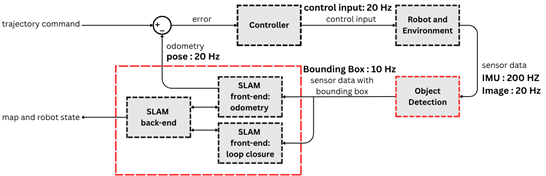
\includegraphics[width=0.9\textwidth]{figures/template/control_loop_rates.png}
  \caption[Scope of the project within the AMR navigation loop.]{Scope of the project within the AMR navigation loop. The red dashed
  frame encloses the blocks this project develops: the SLAM front end
  (odometry and loop closure), the SLAM back end (map and robot state) and the
  object-detection block that supplies bounding boxes. The controller and the
  robot are existing components. Rates are those of the target system: control
  input \SI{20}{\hertz}, odometry pose \SI{20}{\hertz}, bounding boxes
  \SI{10}{\hertz}, IMU \SI{200}{\hertz}, images \SI{20}{\hertz}.}
  \label{fig:scope-architecture}
\end{figure}

\begin{figure}[htbp]
  \centering
  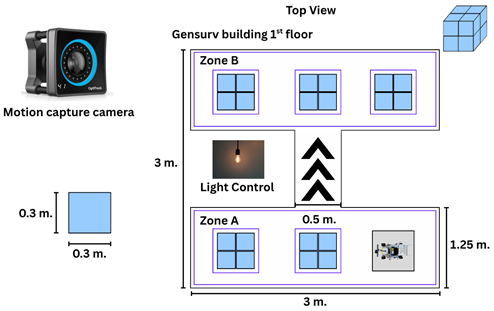
\includegraphics[width=0.8\textwidth]{figures/template/test_field_topview.png}
  \caption[Top view of the mock warehouse test field on the first floor of the Gensurv building.]{Top view of the mock warehouse test field on the first floor of the
  Gensurv building. Zone~A and Zone~B are each \SI{3}{\metre} square and are
  joined by a walkway; the robot starts at the grey square in Zone~A. Goods are
  \SI{0.3}{\metre} cubes stacked in piles, a light-control fixture sets the
  illumination, and motion-capture cameras around the field provide the
  ground-truth reference.}
  \label{fig:test-field}
\end{figure}

\section{Work Plan}
\label{sec:workplan}

\Cref{tab:gantt} reproduces the project work plan of the proposal. Task
numbering follows the original plan, which has no item~5.

\begin{table}[htbp]
\centering
\caption[Work plan for the 2026 (B.E.\ 2569) academic year.]{Work plan for the 2026 (B.E.\ 2569) academic year. Shaded cells mark
the months allocated to each task.}
\label{tab:gantt}
\small
\setlength{\tabcolsep}{3pt}
\newcommand{\gc}{\cellcolor{black!12}}
\begin{tabularx}{\textwidth}{>{\raggedright\arraybackslash}X ccccccc}
\toprule
Task & Jun & Jul & Aug & Sep & Oct & Nov & Dec \\
\midrule
1. Study the concepts and theory of vision-based navigation
  & \gc & \gc & & & & & \\
2. Search and analyse information on visual SLAM algorithms, low-light image
  enhancement (EnlightenGAN), object detection (YOLO26) and lane tracking
  (PolyNET)
  & \gc & \gc & & & & & \\
3. Design the structure and software pipeline that joins the hardware and
  software systems
  & & \gc & \gc & & & & \\
4. Specify and connect the AC-IMX390-H190 camera sensors with the NRU-51V edge
  computing unit on the mobile robot
  & & \gc & \gc & & & & \\
6. Integrate all subsystems under the AMR navigation framework
  & & & \gc & \gc & & & \\
7. Prepare the mock warehouse area (Zone~A and Zone~B) with a \SI{5}{\degree}
  slope and arrange mock goods to create a dynamic environment
  & & & \gc & \gc & & & \\
8. Run the integrated system experiment (live test) with the robot moving at
  \SI{1.5}{\metre\per\second} under scheduled changes in lighting
  & & & & \gc & \gc & & \\
9. Collect the test data and evaluate system performance on the defined
  metrics: trajectory error (ATE, RPE), system latency, and detection accuracy
  (IoU, mAP)
  & & & & & \gc & \gc & \\
10. Summarise the work, discuss the results and produce the complete
  engineering project report
  & & & & & & \gc & \gc \\
\bottomrule
\end{tabularx}
\end{table}

% Chapter 2 is an English rendering of บทที่ 2 ทฤษฎี/งานวิจัยที่เกี่ยวข้อง in the
% faculty template (docs/MyThesisInfo/final_report.pdf, pp. 4-18).  The
% science is the template's; only the language changed.  Figure sources are
% carried over verbatim.
\chapter[THEORY AND RELATED WORK]{Theory and Related Work}
\label{chap:theory}

In carrying out the project ``Vision-Based Navigation Pipeline for AMRs in
Dynamic Warehouse'', the author's aim is to develop and evaluate only the
navigation pipeline, within the scope defined in \cref{sec:scope}. The project
does not set out to build a complete autonomous robot from scratch; it
integrates navigation software into the existing architecture of an autonomous
mobile robot (AMR). To make that development effective, the author studied and
collected theory, documents and research on the following principal topics.

\section{AMR Navigation Systems}
\label{sec:amr-navigation}

Autonomous mobile robots are among the technologies transforming industry in the
digital era, particularly in manufacturing, warehousing and materials handling.
With their capacity to learn, their flexibility and their high precision, AMRs
reduce cost and raise efficiency by a large step. This section reviews the
properties, technology and use cases of AMRs to make the potential of the
innovation clear.

\subsection{Logistics management and the historical bottleneck}

In a traditional warehouse, most wasted expenditure arises in the logistics of
moving material from one point to another, work that exhausts staff who must
walk while continuously carrying loads. These movements produce ``motion waste'',
one of the eight principal wastes of lean manufacturing
(\cref{fig:lean-wastes}). To stay competitive and cut logistics costs, smart
warehouses have begun to bring autonomous robots in to work alongside people
and reduce that time and waste.

\begin{figure}[htbp]
  \centering
  
\includegraphics[width=0.8\textwidth]{figures/template/lean_wastes.png}
  \caption[The eight principal wastes of lean manufacturing.]{The eight principal wastes of lean manufacturing. Source:
  \url{https://teachme-biz.com/th/blog/reduce-waste/}.}
  \label{fig:lean-wastes}
\end{figure}

\subsection{The era of automated guided vehicles (AGVs)}

Research and development of autonomous mobile robots began in the 1950s with
automated guided vehicles. AGV systems have an important limitation: the vehicle
depends on infrastructure installed in the warehouse beforehand for navigation,
such as magnetic tape, QR codes or artificial landmarks
(\cref{fig:agv-navigation}). AGVs can also only follow fixed, pre-planned
routes, so the system lacks spatial flexibility, and if the warehouse
environment changes the AGV cannot adapt immediately.

\begin{figure}[htbp]
  \centering
  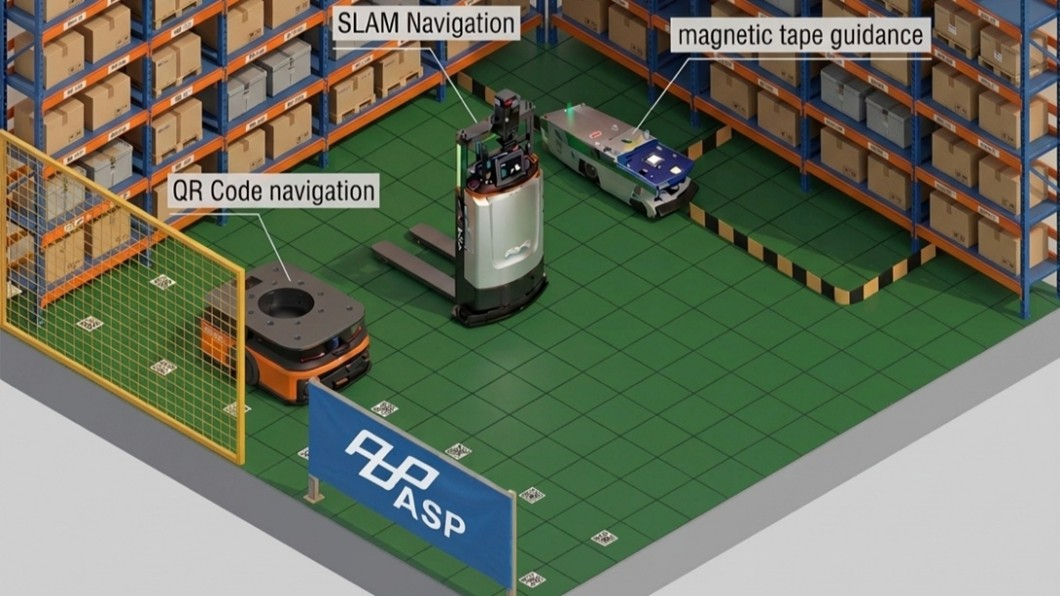
\includegraphics[width=0.8\textwidth]{figures/template/agv_navigation_types.jpg}
  \caption[Three warehouse robots with different navigation technologies: the orange robot uses QR-code navigation, the pallet truck in the centre uses SLAM navigation without floor infrastructure, and the white robot uses magnetic-tape guidance.]{Three warehouse robots with different navigation technologies: the
  orange robot uses QR-code navigation, the pallet truck in the centre uses SLAM
  navigation without floor infrastructure, and the white robot uses
  magnetic-tape guidance. Source:
  \url{https://www.linkedin.com/pulse/agv-amr-navigation-technologies-which-one-drives-your-abdul-rahman-6pjyc}.}
  \label{fig:agv-navigation}
\end{figure}

\subsection{The transition to autonomous mobile robots (AMRs)}

AMRs were developed to overcome the limitations of AGVs. The essential
difference is that an AMR can make its own decisions and does not need
pre-installed external infrastructure to navigate. Recent hardware advances,
particularly in imaging sensors (2-D/3-D cameras and LiDAR) together with
high-performance processors, let an AMR perceive and assess its surroundings
accurately. The distinguishing capability that lets AMRs replace AGVs is
operation in a dynamic environment: when an AMR detects an obstacle on its
route it can compute alternative routes to avoid the obstacle or another robot
automatically, without the user redesigning the route.

With this capacity for independent decision-making and navigation, large
industrial users have moved to AMRs widely. One example is the deployment of
autonomous driverless transport vehicles in the press plant of the BMW Group at
Regensburg~\cite{bmw2024}, whose vehicles navigate and manoeuvre precisely
through busy, complex areas of a real factory (\cref{fig:bmw-agv}), showing that
AMRs have fully overcome the limits of the older navigation systems.

\begin{figure}[htbp]
  \centering
  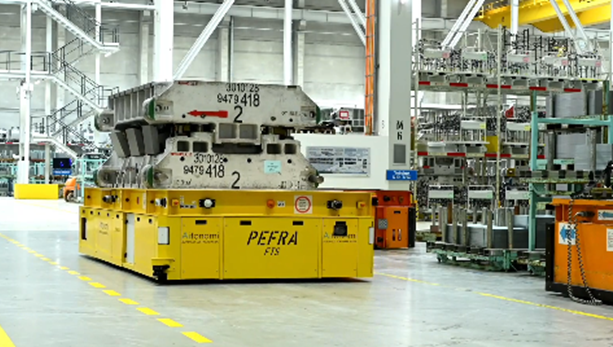
\includegraphics[width=0.7\textwidth]{figures/template/bmw_agv.png}
  \caption[An autonomous driverless transport vehicle navigating precisely in the BMW Group press plant at Regensburg.]{An autonomous driverless transport vehicle navigating precisely in
  the BMW Group press plant at Regensburg. Source:
  \url{https://www.press.bmwgroup.com/global/video/detail/PF0009726/}.}
  \label{fig:bmw-agv}
\end{figure}

\section{Visual Simultaneous Localization and Mapping (Visual SLAM)}
\label{sec:visual-slam}

In the operation of an AMR, localization is the heart of what lets the robot
move accurately. The widely accepted and used method is SLAM (simultaneous
localization and mapping). A SLAM navigation system extracts features present in
the environment to build a map; the software gathers information from the
robot's current position and the positions it has passed through to estimate a
probability distribution and predict the robot's most likely position.

\subsection{Components of a visual SLAM system}

This project concentrates on visual SLAM, mapping and localization with image
sensors, to reduce the cost of LiDAR sensors. Following the project's own
data-flow diagram, a visual SLAM architecture has three main parts
(\cref{fig:slam-indirect}):

\begin{enumerate}[leftmargin=2em]
  \item \textbf{SLAM front end (visual odometry)}: receives camera images and
    extracts features to estimate the robot's relative motion and pose over
    short intervals.
  \item \textbf{SLAM back end}: refines and corrects the accumulated drift of
    the front-end estimate using graph optimisation, to obtain the most accurate
    map and pose.
  \item \textbf{Loop closure}: the process by which the system recognises a
    place the robot has visited before; when the robot returns, the current
    image is matched to a past one and the whole map is corrected to reduce
    accumulated error.
\end{enumerate}

\begin{figure}[htbp]
  \centering
  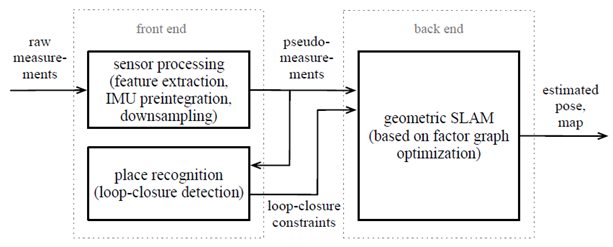
\includegraphics[width=0.85\textwidth]{figures/template/slam_indirect.png}
  \caption{The indirect (feature-based) method common to SLAM systems: a front
  end producing pseudo-measurements and loop-closure constraints, and a back end
  performing geometric SLAM by factor-graph optimisation~\cite{cadena2016}.}
  \label{fig:slam-indirect}
\end{figure}

\subsection{ORB-SLAM3}
\label{sec:theory-orb}

ORB-SLAM3~\cite{campos2021} is an open-source SLAM system that builds on the
success of ORB-SLAM and ORB-SLAM2. It is the first framework to support visual,
visual-inertial and multi-map SLAM with a range of camera types, monocular,
stereo and RGB-D, and with both pinhole and fisheye lens models
(\cref{fig:orbslam3-components}). The parts of its architecture and mechanisms
relevant to this project are as follows.

\begin{figure}[htbp]
  \centering
  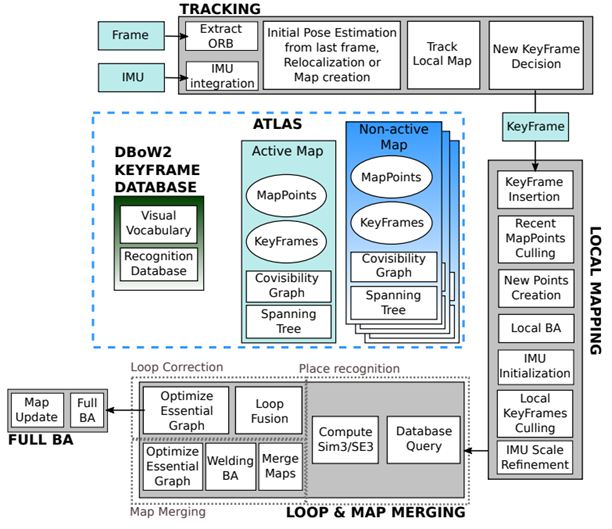
\includegraphics[width=0.8\textwidth]{figures/template/orbslam3_components.png}
  \caption{Main components of ORB-SLAM3: the tracking, local mapping and loop
  and map-merging threads around the Atlas multi-map representation and the
  DBoW2 keyframe database~\cite{campos2021}.}
  \label{fig:orbslam3-components}
\end{figure}

\subsubsection{Tightly-coupled visual-inertial SLAM}

One of the most important advances of ORB-SLAM3 is its visual-inertial SLAM
(VI-SLAM), which fuses data tightly by maximum-a-posteriori (MAP) estimation
both during initialisation and in normal operation, unlike earlier systems that
separated the computations. Its mechanisms are:

\begin{itemize}[leftmargin=2em]
  \item \textbf{Fast IMU initialisation.} The main problem of typical VI-SLAM
    systems is the delay in computing the IMU's initial parameters. ORB-SLAM3
    proposes a MAP uncertainty computation that recovers the map scale, the
    gravity direction and the gyroscope and accelerometer biases within about
    two seconds of start-up, so the robot obtains a correct pose with a
    physically true distance scale immediately.
  \item \textbf{Joint local bundle adjustment.} While moving, the system solves
    for the robot pose together with the 3-D landmarks and the IMU states
    (velocity and biases) simultaneously within a local window, compensating
    the accumulated drift of the images and the inertial sensor effectively.
\end{itemize}

\subsubsection{Atlas: multi-map system and place recognition}

To support lifelong mapping in an environment that changes or has visual
disturbances, such as a dynamic warehouse, ORB-SLAM3 introduces the Atlas map
management architecture, holding maps in two states:

\begin{itemize}[leftmargin=2em]
  \item \textbf{Active map}: the local sub-map the robot is currently using for
    tracking and mapping.
  \item \textbf{Non-active maps}: the set of past sub-maps the system has
    recorded and kept in memory.
\end{itemize}

When the robot passes through severe occlusion, or the lighting changes so far
that the camera cannot follow the previous features (tracking lost), an ordinary
SLAM system usually fails and stops. ORB-SLAM3 instead moves the map that lost
tracking into the non-active set and immediately starts a new active map to
continue localizing. When the robot later returns to a previously mapped area,
the place-recognition algorithm, with its improved recall, detects the overlap
and triggers map merging of the current active map with the earlier non-active
map, correcting the error by loop closure. This mechanism permanently reduces
the risk of the robot becoming lost in the warehouse.

\subsubsection{Abstract camera representation for wide-angle lenses}

Because this project selects the AC-IMX390-H190 camera with an ultra-wide
\SI{186}{\degree} field of view (fisheye lens), ORB-SLAM3 is technically well
suited: its architecture places an abstract representation layer between the
feature extractor and the camera projection model, so the system can switch to
the Kannala--Brandt fisheye model directly without affecting the back-end SLAM
algorithms. The robot can therefore process wide-angle images correctly and
without distortion in the localization result.

\subsection{VINS (Visual-Inertial System)}
\label{sec:theory-vins}

VINS (VINS-Mono, VINS-Fusion)~\cite{qin2018vins} is a high-performance
open-source state estimator developed by the Aerial Robotics Group (HKUST). Its
extended versions can fuse GPS, but for this project's indoor dynamic warehouse
VINS is used as a local 6-DoF visual-inertial odometry (VIO) estimator
(\cref{fig:vins-components}). Its main mechanisms are as follows.

\begin{figure}[htbp]
  \centering
  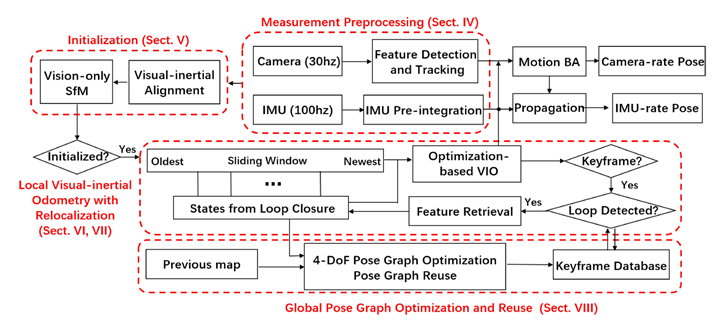
\includegraphics[width=0.95\textwidth]{figures/template/vins_components.png}
  \caption{Main components of monocular VINS: measurement preprocessing,
  initialisation, sliding-window visual-inertial odometry with relocalization,
  and global pose-graph optimisation and reuse~\cite{qin2018vins}.}
  \label{fig:vins-components}
\end{figure}

\subsubsection{IMU pre-integration}

In a fused sensor system the accelerometer and gyroscope deliver data at a very
high rate (\SIrange{100}{200}{\hertz}) while the camera delivers images at a
lower one (\SIrange{20}{30}{\hertz}). If a SLAM system re-integrated the IMU data
every time a pose was adjusted, the computational load would be enormous. VINS
solves this with IMU pre-integration: the accelerations and angular rates
between two consecutive image frames are integrated in the robot's local body
frame rather than the global frame, so the pre-integrated measurements do not
depend on the initial state and need not be recomputed when the back end
corrects the robot's pose. The system also propagates covariance and corrects
gyroscope and accelerometer bias through a first-order Taylor expansion, giving
a physically accurate pose estimate.

\subsubsection{Robust estimator initialisation}

A central challenge of visual-inertial SLAM is initialisation, because
monocular or stereo images carry no true metric scale at the outset and the IMU
carries accumulated bias. VINS establishes a tightly-coupled initialisation in
two steps:

\begin{itemize}[leftmargin=2em]
  \item \textbf{Local structure from motion (SfM).} Features are extracted and
    tracked over a window of time to build a 3-D structure and the relative
    camera poses first.
  \item \textbf{Visual-inertial alignment.} The SfM trajectory is set against
    the IMU pre-integration results to recover three initial quantities: the
    metric scale, the gravity direction relative to the robot, and the initial
    gyroscope bias. The AMR thereby perceives true metric distances in the
    warehouse immediately after it begins to move.
\end{itemize}

\subsubsection{Tightly-coupled sliding-window optimisation}

At the heart of the VINS pipeline is a sliding window that limits the number of
image frames and robot states that must be solved for. VINS forms a nonlinear
least-squares cost function, solved with Ceres Solver, in which three residuals
are tightly coupled:
\begin{equation}
  \min_{\chi}\Bigl\{\bigl\lVert r_p - H_p\chi\bigr\rVert^2
  + \sum_{k\in\mathcal{B}}\bigl\lVert r_{\mathcal{B}}\bigl(\hat{z}^{b_k}_{b_{k+1}},\chi\bigr)\bigr\rVert^2_{P^{b_k}_{b_{k+1}}}
  + \sum_{(l,j)\in\mathcal{C}}\bigl\lVert r_{\mathcal{C}}\bigl(\hat{z}^{c_j}_l,\chi\bigr)\bigr\rVert^2_{P^{c_j}_l}\Bigr\},
  \label{eq:vins-cost}
\end{equation}
where
\begin{itemize}[leftmargin=2em]
  \item the \textbf{marginalisation residual} $r_p$ is the prior obtained from
    past frames removed from the sliding window;
  \item the \textbf{IMU residual} $r_{\mathcal{B}}$ is the error between the
    robot's true state and the IMU pre-integration; and
  \item the \textbf{visual re-projection residual} $r_{\mathcal{C}}$ is the
    re-projection error of feature points on the stereo image plane.
\end{itemize}

\subsubsection{Marginalisation for real-time load control}

To keep the edge processor (NRU-51V) on the robot running in real time, VINS
removes frames from the sliding window under two conditions:

\begin{itemize}[leftmargin=2em]
  \item \textbf{Marginalise old (\texttt{MARGIN\_OLD}).} If the newest frame is
    judged a keyframe, the oldest frame in the window is removed, and its
    visual and inertial information is converted into a prior factor by the
    Schur complement so that important past parameters are not lost.
  \item \textbf{Marginalise second newest (\texttt{MARGIN\_SECOND\_NEW}).} If
    the newest frame is judged a non-keyframe (insufficient parallax), the
    second-newest frame is discarded outright without forming a prior. This
    bounds the density of the matrices and saves a great deal of computation
    when the AMR is stationary or moving slowly in the warehouse.
\end{itemize}

\subsubsection{Online temporal calibration}

A distinctive feature of VINS~\cite{qin2018td} is its treatment of temporal
misalignment between the camera and the IMU. In practice the camera trigger and
the IMU signals suffer transmission and triggering delays, so the two sensors'
timestamps disagree, an important cause of VIO failure when the robot moves fast
or turns. VINS adds the time offset as a state variable estimated jointly in the
back-end optimisation, computing the temporal shift of the image frames against
the IMU angular rate. The pipeline can thereby compensate the latency of the
AC-IMX390-H190 image stream on the processing board precisely, keeping tracking
consistent even when the robot vibrates on the \SI{5}{\degree} warehouse slope.

\subsection{RTAB-Map back end and memory management}
\label{sec:theory-rtab}

Following Labbé and Michaud~\cite{labbe2019}, RTAB-Map is an open-source SLAM
library designed to avoid failure through computational and memory explosion
when a robot operates over a large area or for a long time (lifelong mapping).
RTAB-Map receives odometry and point-cloud data from VINS and performs graph
SLAM in the back end through three main mechanisms
(\cref{fig:rtabmap-components}).

\begin{figure}[htbp]
  \centering
  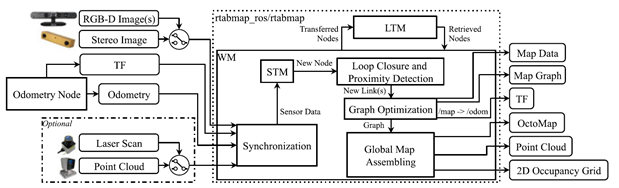
\includegraphics[width=0.95\textwidth]{figures/template/rtabmap_components.png}
  \caption{Main components of RTAB-Map: sensor synchronisation, short-term and
  working memory, long-term memory, loop-closure and proximity detection, graph
  optimisation and global map assembly~\cite{labbe2019}.}
  \label{fig:rtabmap-components}
\end{figure}

\subsubsection{Memory partitioning modelled on human memory}

RTAB-Map does not keep and compute over every map node in RAM; it organises the
data on three levels:

\begin{itemize}[leftmargin=2em]
  \item \textbf{Short-term memory (STM)} receives the latest image and odometry
    from VINS, extracts features and creates a new node. Nodes in STM are not
    yet used for loop-closure computation.
  \item \textbf{Working memory (WM)} is the main RAM area in which the
    algorithm detects loop closures and performs graph optimisation. The WM size
    is held constant by a time threshold so that the computation time never
    exceeds the real-time limit (for example \SI{<30}{\milli\second}).
  \item \textbf{Long-term memory (LTM)} is the database written to permanent
    storage (SSD or hard disk). Its contents do not enter the ordinary graph
    optimisation, conserving RAM and CPU.
\end{itemize}

\subsubsection{Memory transfer and weighting heuristics}

To lock the processing time at a constant ($O(1)$ time complexity) regardless
of how large the warehouse map becomes, RTAB-Map moves data between WM and LTM
as follows:

\begin{itemize}[leftmargin=2em]
  \item \textbf{Node weighting.} When the robot traverses a previous route and a
    loop closure occurs, the nodes there gain weight; frequently traversed nodes
    (such as the main warehouse aisles) carry high weight.
  \item \textbf{WM-to-LTM transfer.} When WM processing time approaches the set
    limit, the algorithm forces the ``oldest and least-weighted'' nodes out of
    RAM into LTM temporarily.
  \item \textbf{LTM-to-WM retrieval.} If the robot returns to an old area and
    feature extraction finds a link to a past node, the algorithm automatically
    retrieves the neighbouring nodes from LTM back into WM to connect the map
    structure and correct accumulated drift.
\end{itemize}

\subsubsection{Memory-constrained graph optimisation}

Unlike ordinary SLAM systems, which must optimise the graph over the whole map
and stall when run for a long time, RTAB-Map optimises the graph (through g2o or
GTSAM) only over the nodes remaining in working memory. The NRU-51V edge
processor can therefore run the navigation system and update the warehouse map
smoothly over its whole service life without loss of speed.

\section{Real-Time Object Detection}
\label{sec:object-detection}

\subsection{The role of object detection in semantic understanding}

In traditional geometric visual SLAM the algorithm extracts geometric features
without knowing what kind of object they belong to. For a warehouse that
changes continually, geometry alone is not enough: the system needs semantic
understanding to distinguish permanent structure from movable dynamic obstacles
(goods, pallets, people). This project therefore integrates object detection
into the front end to produce bounding boxes and pass the coordinates of dynamic
objects to the SLAM system, which masks out the unstable features.

\subsection{The YOLO (You Only Look Once) network architecture}

For the system to respond in real time while the SLAM system is running, the
project concentrates on the YOLO family, a one-stage detector distinguished by
its processing speed. Unlike two-stage models (such as Faster R-CNN) that first
generate region proposals and then classify them, YOLO predicts bounding-box
regression and class probabilities for the whole image in a single forward pass,
which makes YOLO (for example YOLO26) well suited to deployment on a
resource-limited edge processor such as the NRU-51V board.
\Cref{tab:detector-comparison} compares the main detector architectures.

\begin{table}[htbp]
\centering
\caption{Comparison of object-detection model architectures.}
\label{tab:detector-comparison}
\small
\setlength{\tabcolsep}{4pt}
\begin{tabularx}{\textwidth}{>{\raggedright\arraybackslash}p{0.14\textwidth}>{\raggedright\arraybackslash}p{0.13\textwidth}>{\raggedright\arraybackslash}X>{\raggedright\arraybackslash}X>{\raggedright\arraybackslash}p{0.18\textwidth}}
\toprule
Architecture & Category & Main strengths & Limitations & Suitable use \\
\midrule
Faster R-CNN & Two-stage detector & Excels in classification and localization,
  achieving high mAP and IoU with a low overall error rate and high spatial
  accuracy & The multi-stage process slows inference & Work requiring high
  accuracy without real-time processing \\
YOLO series & Single-stage detector & Casts detection as a single-stage
  regression problem tuned for speed, balancing speed and accuracy well, with
  high precision and recall and a low false-positive rate & Although now well
  refined, early versions had trouble with small or densely clustered objects
  compared with two-stage models & Real-time work requiring high processing
  speed and low latency \\
SSD (Single Shot Detector) & Single-stage detector & Removes the region-proposal
  step and performs multi-scale detection within one network & Sometimes
  slightly slower than YOLO, but still very efficient & Applications needing a
  reliable balance of throughput and accuracy \\
MobileNet / EfficientNet & Lightweight model & Uses techniques such as
  depthwise-separable convolutions to cut parameters and computation
  substantially without reducing learning capacity & Overall accuracy may be
  below large models such as Faster R-CNN or the larger YOLO versions & Edge
  devices with limited memory and compute: smartphones, IoT devices, drones \\
\bottomrule
\end{tabularx}
\end{table}

\subsection{Performance evaluation and edge-processor limits}

In bringing a YOLO model into a visual SLAM pipeline, the essential point is the
trade-off between accuracy and inference time (latency): too large a model
creates a bottleneck and makes the SLAM system fall behind the camera frame
rate. The evaluation of the YOLO model on a simulated warehouse dataset, through
a platform such as Roboflow, therefore uses the following main metrics:

\begin{itemize}[leftmargin=2em]
  \item \textbf{Intersection over union (IoU)}: the overlap ratio between the
    predicted box and the true object box, measuring localization accuracy.
  \item \textbf{Precision}: the fraction of dynamic-object predictions that are
    correct, out of all dynamic-object predictions (accuracy of the prediction).
  \item \textbf{Recall}: the fraction of dynamic objects correctly predicted, out
    of all dynamic objects actually present in the image (coverage of the
    search).
  \item \textbf{F1 score}: the harmonic mean of precision and recall, measuring
    the model's balance.
  \item \textbf{Average precision (AP) and mean average precision (mAP)}: the
    overall accuracy reflecting the model's combined performance across all
    object types under differing confidence thresholds.
\end{itemize}

Choosing the model with the highest mAP that still keeps latency within a safe
budget (for example \SIrange{<15}{20}{\milli\second}) is the key to a complete
integration of YOLO and SLAM.

\section{RY-SLAM: A Robust YOLO-Based Real-Time Visual SLAM Solution for
Dynamic Environments}
\label{sec:ryslam}

\subsection{Concept and architecture of RY-SLAM}

Chen et al.~\cite{chen2025} present RY-SLAM (Robust YOLO SLAM), an advanced
visual SLAM system designed to solve navigation failure in dynamic
environments. RY-SLAM integrates the ORB-SLAM3 framework with a YOLO-family
semantic detection and segmentation network (for example YOLOv8s-seg). Its
architecture relies on multi-threaded parallel processing with GPU
acceleration: the semantic-segmentation thread is separated from the SLAM
tracking thread, so the system can analyse dynamic-object coordinates and
estimate the camera pose at the same time without losing real-time throughput
(\cref{fig:ryslam-architecture}).

\begin{figure}[htbp]
  \centering
  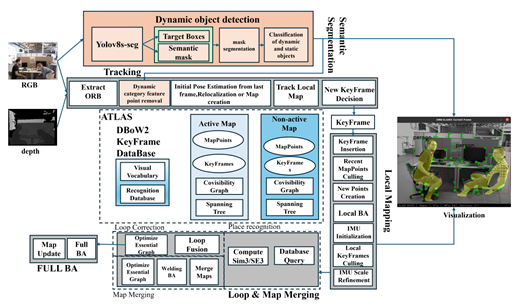
\includegraphics[width=0.9\textwidth]{figures/template/ryslam_architecture.png}
  \caption{Architecture of RY-SLAM: a YOLOv8-seg dynamic-object detection stage
  feeding a semantic mask into the ORB-SLAM3 tracking thread ahead of the Atlas
  multi-map system~\cite{chen2025}.}
  \label{fig:ryslam-architecture}
\end{figure}

\subsection{Dynamic feature masking mechanism}

The heart of RY-SLAM's localization accuracy is its dynamic feature masking,
in three technical steps:

\begin{itemize}[leftmargin=2em]
  \item \textbf{Semantic mask generation.} The YOLO model analyses the input
    frame to detect dynamic objects (such as people or vehicles) and generates
    a mask around each object's area.
  \item \textbf{Outlier elimination.} In the ORB-SLAM3 feature-extraction step
    the system checks the position of each ORB feature; any feature falling
    inside a dynamic-object mask is deleted immediately.
  \item \textbf{Static pose estimation.} Only features extracted from the
    permanent structure of the environment (static background) are fed to
    bundle adjustment, reducing accumulated drift and tracking loss
    significantly compared with standard ORB-SLAM3.
\end{itemize}

\begin{figure}[htbp]
  \centering
  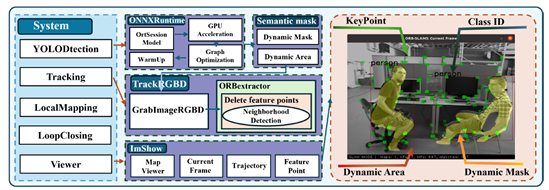
\includegraphics[width=0.9\textwidth]{figures/template/ryslam_framework.png}
  \caption[Detail of the semantic-segmentation framework in RY-SLAM and its multi-threaded operation: ONNX Runtime inference producing the dynamic mask, the neighbourhood test that deletes feature points, and the viewer outputs~\cite{chen2025}.]{Detail of the semantic-segmentation framework in RY-SLAM and its
  multi-threaded operation: ONNX Runtime inference producing the dynamic mask,
  the neighbourhood test that deletes feature points, and the viewer
  outputs~\cite{chen2025}.}
  \label{fig:ryslam-framework}
\end{figure}

\subsection{Relevance to this project}

RY-SLAM is important academic evidence for the effectiveness and soundness of
combining a YOLO-family model with ORB-SLAM3. For this project the author adopts
the basic concept and architecture of RY-SLAM and develops it further in
pipeline~1 (YOLO26 + ORB-SLAM3), raising system performance by choosing the
newer YOLO26 model to filter obstacles and mock goods in the warehouse in real
time, together with the Atlas multi-map architecture of ORB-SLAM3 on the NRU-51V
edge processor, so as to build a navigation system that is robust both to
close-proximity dynamic objects and in long-term (lifelong) mapping, as the
objectives require.

% Chapter 3.  The storytelling order is that of the 23 September 2026 progress
% update: problem and scope -> architecture -> the two pipelines -> simulation
% platform -> real platform -> the four experiments -> evaluation -> what
% changed from the plan.  Hardware, site and procedure paragraphs are English
% renderings of บทที่ 3 of the faculty template; every "as implemented" passage
% is a verbatim fragment of the retired minor report (chapters/fragments/),
% whose numbers were checked against the repository.
\chapter[METHODOLOGY]{Methodology}
\label{chap:methodology}

To let the system solve the problem set out in \cref{chap:introduction} and be
deployed on an edge AI computer, this project integrates a neural object
detector (YOLO26) into the core of a visual SLAM framework, a combination
referred to as semantic visual SLAM. This chapter describes the problem and its
scope, the system architecture, the two navigation pipelines as they were
actually built, the simulation and real platforms, the four experiments that
structure the evaluation, the metrics, and the points at which the implemented
system departs from the method originally proposed.

\textbf{Reporting cutoff.} Every implementation claim in this chapter describes
the repository at 25 September 2026. Components are labelled
\status{implemented}, \status{partial}, \status{blocked} or \status{planned};
nothing planned is described in the present tense as though it existed.

\section{Problem, Requirements and Scope}
\label{sec:problem-scope}

The engineering problem is to localize a warehouse AMR with cameras and an IMU,
without floor infrastructure, in an environment whose contents move. The
company's present LiDAR-and-QR-code navigation is accurate but expensive to
install and inflexible (\cref{sec:background}); a camera-based replacement is
attractive only if it stays accurate when goods, pallets and people move
through the field of view, which is exactly the case standard visual SLAM
assumes away.

\textbf{Performance targets.} The project states two trajectory targets for the
integrated system at the robot's working speed of \SI{1.5}{\metre\per\second}:
an absolute trajectory error of at most \SI{0.05}{\metre}, and a relative pose
error over \SI{1}{\second} of at most \SI{1.5}{\metre}. The original objective
list (\cref{sec:objectives}) states the localization requirement as an error
below \SI{10}{\centi\metre} under differing illumination. Both figures are
carried into \cref{chap:results} and every trajectory result is read against
them.

\textbf{Site.} The real tests take place on the first floor of the Gensurv
building, in a mock warehouse of roughly \SI{10}{\metre} by \SI{7}{\metre}
divided into two operating zones, Zone~A and Zone~B, each about
\SI{3}{\metre} square and joined by a walkway (\cref{fig:test-field}). The
walkway carries a \SI{5}{\degree} slope. Goods are \SI{0.3}{\metre} cubes in
stacks whose positions are changed between runs, and a light-control fixture
sets the illumination to a schedule. A motion-capture system provides the
ground-truth reference (\cref{sec:real-site}).

\textbf{Two domains.} Every experiment is defined once and run twice, in a
Gazebo simulation of the warehouse and on the real robot. The simulation
supplies exact ground truth, exact calibration and repeatable dynamic scenes;
the real robot supplies the sensors, the lighting and the physics the project
is ultimately about. The two domains are never pooled.

\textbf{What is excluded.} Path planning and motion control are outside the
project: the pipeline delivers a pose and a map to an existing planner and
controller (\cref{fig:scope-architecture}). Of the five original objectives,
this report addresses objectives~1, 3 and~5 (visual-inertial localization with
mapping, dynamic-object detection, and the integrated localization
requirement). Objective~2 (EnlightenGAN low-light enhancement) and objective~4
(PolyNET lane detection with PID lane tracking) were not pursued within the
reporting period and are recorded as deviations in \cref{sec:deviations}.

\section{System Architecture}
\label{sec:architecture}

\subsection{Control-loop view and data rates}

\Cref{fig:scope-architecture} places the project inside the AMR's control loop.
The controller issues control input at \SI{20}{\hertz}; the SLAM front end
returns an odometry pose at \SI{20}{\hertz}; the object detector returns
bounding boxes at \SI{10}{\hertz} on the real robot; the IMU streams at
\SI{200}{\hertz} and the cameras at \SI{20}{\hertz}. In simulation the cameras
run at \SI{30}{\hertz} and detections are produced per frame, and the wheel
odometry of the simulated platform is published at \SI{50}{\hertz}
(\cref{tab:platform-geometry}). The four experiments of \cref{sec:experiments}
are each located on one block of this loop:

\begin{table}[htbp]
\centering
\caption{The four experiments and the architecture block each one tests.}
\label{tab:experiment-map}
\small
\begin{tabularx}{\textwidth}{c>{\raggedright\arraybackslash}p{0.40\textwidth}>{\raggedright\arraybackslash}X}
\toprule
\# & Experiment & Block under test \\
\midrule
1 & Non-visual baseline and estimator comparison & the robot's own odometry
  against the SLAM output: is vision earning its place? \\
2 & Offline YOLO detector performance & the object-detection block, in
  isolation \\
3 & Visual-inertial odometry with dynamic-environment filtering & the SLAM
  front end, with and without the detector's mask \\
4 & Dense map reconstruction and map-quality evaluation & the SLAM back end and
  the map it delivers \\
\bottomrule
\end{tabularx}
\end{table}

\subsection{Semantic visual SLAM data flow}

The architecture is organised in two parts, front-end sensor processing and
back-end SLAM and mapping.

\begin{itemize}[leftmargin=2em]
  \item \textbf{Front-end processing pipeline.}
    \emph{Sensor data ingestion} receives raw images from the wide-angle stereo
    cameras (Sony IMX390, \SI{186}{\degree} field of view) together with
    acceleration and angular rate from the IMU, through ROS~2 nodes. The
    \emph{dynamic object detection module} passes each image to the YOLO26
    model to detect, in real time, movable warehouse objects (goods, pallets,
    people) and emits their bounding boxes. The \emph{dynamic feature masking
    protocol} compares those boxes with the geometric keypoints extracted by
    the SLAM front end (ORB or FAST corners); any keypoint that falls inside a
    dynamic object's box is masked and discarded, so that only features of the
    permanent warehouse structure remain.
  \item \textbf{Back-end SLAM and mapping.} The filtered features enter
    odometry and graph optimisation to estimate the 6-DoF robot state, update
    the 3-D point map of the permanent structure, and build the 2-D occupancy
    grid the navigation system consumes.
\end{itemize}

\Cref{fig:system-architecture} shows the data flow of the system as it exists.

% Verbatim from minor_report/chapters/chapter_3_methodology.tex lines 24-43 (retired report),
% headings demoted by 0 level(s). Do not edit here; edit the source of the numbers.

\begin{figure}[htbp]
  \centering
  \resizebox{\textwidth}{!}{% Experimental architecture. Nodes are placed on an explicit grid rather than by
% relative chaining: the detector sits between the two estimators so that its two
% optional edges are short verticals instead of connectors routed through the
% estimator boxes, and every arrow enters a distinct face of its target node.
% The trajectory-to-RTAB-Map gap is sized to hold its edge label clear of both
% boxes and of the grouping rectangle.
\begin{tikzpicture}[
  block/.style={draw, rounded corners, align=center, minimum height=9mm,
    text width=34mm, font=\footnotesize, fill=implemented, inner sep=2mm},
  source/.style={block, fill=gray!15},
  backend/.style={block, fill=external},
  plan/.style={block, fill=planned, dashed},
  flow/.style={-{Latex[length=2.2mm]}, thick},
  optional/.style={flow, dashed},
  edgelabel/.style={font=\scriptsize, fill=white, inner sep=1.5pt}
]
  \node[source]  at ( 0.0,  0.0) (sensors)    {Stereo images\\and IMU};
  \node[block]   at ( 5.0,  2.8) (vins)       {VINS-Fusion\\track culling and\\feature suppression};
  \node[block]   at ( 5.0,  0.0) (detector)   {Optional YOLO\\box detector};
  \node[block]   at ( 5.0, -2.8) (orb)        {ORB-SLAM3\\feature rejection};
  \node[source]  at (10.2,  0.0) (trajectory) {Common trajectory\\\texttt{vio.csv}};
  \node[backend] at (16.6,  0.0) (rtab)       {RTAB-Map\\external back end};
  \node[source]  at (10.2, -5.0) (evaluation) {Trajectory and\\map evaluation};
  \node[plan]    at (16.6, -5.0) (future)     {Planned integrated\\relocalization, global\\optimization, map merging};

  % Sensor stream reaches the detector and both estimators without crossings.
  \draw[flow] (sensors.east) -- (vins.west);
  \draw[flow] (sensors.east) -- (detector.west);
  \draw[flow] (sensors.east) -- (orb.west);

  % Optional masks: short verticals, so nothing is drawn across a box.
  \draw[optional] (detector.north) -- (vins.south);
  \draw[optional] (detector.south) -- (orb.north);

  % Both estimators write the common trajectory; they enter the two left corners
  % so the arrowheads stay apart and the south face is free for the next edge.
  \draw[flow] (vins.east) -- (trajectory.north west);
  \draw[flow] (orb.east) -- (trajectory.south west);
  \draw[flow] (trajectory.south) -- (evaluation.north);
  \draw[flow] (trajectory.east) -- node[edgelabel]{TF odometry} (rtab.west);
  \draw[flow] (rtab.south west) -- (evaluation.east);
  \draw[optional] (rtab.south) -- (future.north);

  \node[draw, fit=(vins)(orb)(trajectory), inner sep=3mm,
    label={[font=\scriptsize]above:front-end trajectory path}] {};
\end{tikzpicture}
}
  \caption[Implemented experimental architecture.]{Implemented experimental architecture. Green blocks are implemented
  project components, blue denotes the external RTAB-Map back end, and the dashed
  yellow block is future work. The diagram deliberately does not show a feedback
  connection from RTAB-Map into either front end because that integration has not
  been implemented.}
  \label{fig:system-architecture}
\end{figure}

As shown in \cref{fig:system-architecture}, the current work contains two related
but separate evaluation paths. The first measures front-end trajectory behaviour
with and without semantic feature filtering. The second studies map reconstruction
and external global correction through RTAB-Map. RTAB-Map's
\texttt{map~$\rightarrow$~odom} transform does not modify the internal feature map,
state history, or previously recorded trajectory of ORB-SLAM3 or VINS-Fusion. A
unified architecture for relocalization, global optimization, and multi-session
map merging is \status{planned}, not implemented. Path planning is outside the
present research scope.


% Verbatim from minor_report/chapters/chapter_3_methodology.tex lines 45-101 (retired report),
% headings demoted by 0 level(s). Do not edit here; edit the source of the numbers.

\begin{longtable}{>{\raggedright\arraybackslash}p{0.30\textwidth}
                  >{\raggedright\arraybackslash}p{0.23\textwidth}
                  >{\raggedright\arraybackslash}p{0.39\textwidth}}
\caption{Implementation status at the reporting cutoff.}
\label{tab:implementation-status}\\
\toprule
Component & Status & Scope of evidence \\
\midrule
\endfirsthead
\toprule
Component & Status & Scope of evidence \\
\midrule
\endhead
Warehouse simulation and controlled worlds & \status{Implemented; verified} &
Static, dynamic, textured-floor, and featureless-floor world and launch files are
present. \\
ORB-SLAM3 ROS~2 stereo-inertial wrapper & \status{Implemented; verified in
simulation} & Live topics, worker-thread tracking, TF, and common trajectory
output are implemented. \\
ORB-SLAM3 semantic filtering & \status{Implemented; mechanism verified} &
Detector messages reach the tracker and masked ORB candidates are rejected before
octree distribution. \\
VINS-Fusion stereo-inertial estimator & \status{Implemented} & Simulation and
real-rig configurations, odometry publication, TF, and trajectory output are
present. \\
VINS-Fusion semantic filtering & \status{Implemented; mechanism verified} &
Existing KLT tracks are culled and new features are suppressed in detected
regions. \\
Offline YOLO evaluation & \status{Implemented; partially evaluated} &
Ground-truth projection, IoU matching, per-frame CSV files, and validation
overlays are present. \\
RTAB-Map construction and saved-map localization & \status{Implemented; partially
verified} & Construction and basic read-only localization passed; one tiny-map
database has been quantitatively evaluated for geometry and drivability
(\cref{sec:map-quality}). Arbitrary-start aliasing rejection and the
large-warehouse evaluation have not been done. \\
RTAB-Map extend and multi-session merging & \status{Implemented at launch level;
experimentally unverified} & The mode exists, but the planned Level~4 experiment
has not been completed. \\
Live VINS-Fusion and RTAB-Map co-execution & \status{Blocked} & VINS diverges under
the combined workload on the current computer; the mechanism is unresolved. \\
RPE and complete compute evaluation & \status{Partially implemented} & Front-end,
back-end, local-mapping, loop-closing, delivery/state, cumulative process CPU,
and resident-memory records are now logged. RPE was added after the cutoff and
applied to the campaign (\cref{sec:rpe}). External-process monitoring and the
repeated hardware matrix remain planned. \\
\bottomrule
\end{longtable}

The repository state used for this draft is superproject commit
\repo{4425a415f624d6a45da1da4f3b2404cbf7914197}. The checked-out submodules are
VINS-Fusion \repo{4a2223c9e54dfc5d2e94eb2ec1dfc8fd3b8045bb}, RTAB-Map ROS
\repo{56064e4388f6f3ad6b994dbff98bcc0a41488102}, and the warehouse environment
\repo{3df54c6e6ec267fad204e208db61c4ab491be410}. The ORB-SLAM3 core is pinned to
\repo{5c2b00f732775f78836751dba13db25463a0aaa1}. The VINS-Fusion worktree contains
an uncommitted output-directory creation fix at the cutoff; this must be committed
or otherwise recorded before a reproducibility release.


\subsection{The two navigation pipelines compared}
\label{sec:pipelines-compared}

The project compares two pipeline architectures built on that front end.

\textbf{Pipeline~1: YOLO26 + ORB-SLAM3 (Atlas multi-map system).} A
tightly-coupled visual-inertial SLAM that performs both odometry and map
construction through one graph. Lifelong mapping relies on ORB-SLAM3's Atlas
framework: when tracking is lost because the environment changed, the system
opens a new active map and keeps the old one as non-active; when the robot
returns to a known area the maps are merged and joined by loop closure across
maps. Its strength is high accuracy from tight image--IMU fusion, suited to
areas with clear geometric features (\cref{fig:pipeline1}).

\textbf{Pipeline~2: YOLO26 + VINS + RTAB-Map (decoupled VIO and memory
management).} A decoupled architecture that separates high-rate front-end
odometry from long-term back-end memory management. The front end runs VINS
sliding-window visual-inertial odometry on the static features from YOLO26,
giving low-latency odometry that remains stable when the robot vibrates or
drives the \SI{5}{\degree} slope. Lifelong mapping is handled by RTAB-Map, which
holds its working memory at a constant size to bound computation time and moves
old nodes to long-term memory on disk. Its strength is stable use of hardware
resources: it prevents RAM exhaustion on a small processing board during long
continuous operation (\cref{fig:pipeline2}).

\begin{figure}[htbp]
  \centering
  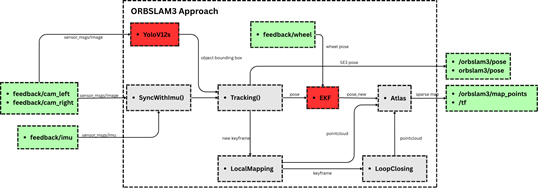
\includegraphics[width=\textwidth]{figures/template/pipeline1_orb.png}
  \caption[Pipeline~1, YOLO26 + ORB-SLAM3, as designed: stereo images and IMU are synchronised, tracked and passed to local mapping, loop closing and the Atlas map; the detector's boxes enter the tracking stage.]{Pipeline~1, YOLO26 + ORB-SLAM3, as designed: stereo images and IMU
  are synchronised, tracked and passed to local mapping, loop closing and the
  Atlas map; the detector's boxes enter the tracking stage. The EKF block that
  fuses the SLAM pose with wheel feedback is a planned integration point and is
  not exercised in this report.}
  \label{fig:pipeline1}
\end{figure}

\begin{figure}[htbp]
  \centering
  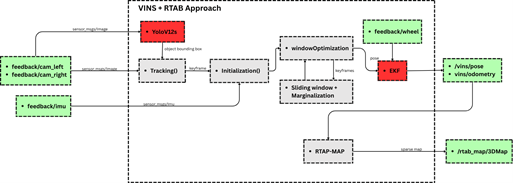
\includegraphics[width=\textwidth]{figures/template/pipeline2_vins_rtab.png}
  \caption[Pipeline~2, YOLO26 + VINS + RTAB-Map, as designed: VINS tracking, initialisation and sliding-window optimisation produce odometry, RTAB-Map builds the map from that odometry and the stereo images.]{Pipeline~2, YOLO26 + VINS + RTAB-Map, as designed: VINS tracking,
  initialisation and sliding-window optimisation produce odometry, RTAB-Map
  builds the map from that odometry and the stereo images. As in
  \cref{fig:pipeline1}, the EKF fusion with wheel feedback is planned.}
  \label{fig:pipeline2}
\end{figure}

\begin{table}[htbp]
\centering
\caption{Design comparison of the two pipeline architectures, as proposed.}
\label{tab:pipeline-comparison}
\small
\begin{tabularx}{\textwidth}{>{\raggedright\arraybackslash}p{0.26\textwidth}>{\raggedright\arraybackslash}X>{\raggedright\arraybackslash}X}
\toprule
Aspect & Pipeline~1: YOLO26 + ORB-SLAM3 & Pipeline~2: YOLO26 + VINS + RTAB-Map \\
\midrule
System structure & tightly coupled (centralised) & decoupled (odometry separate
  from back end) \\
Odometry & ORB-SLAM3 tracking thread; tightly-coupled MAP estimation over
  visual and IMU terms & VINS-Fusion local VIO; sliding-window optimisation \\
Lifelong-mapping mechanism & Atlas multi-map system and map merging
  ($\mathrm{Sim}(3)$) & RTAB-Map memory management (WM / LTM node transfer) \\
Computation-time bound & grows with the number of keyframes and sub-maps in
  Atlas & held at a constant $O(1)$ ceiling in working memory \\
RAM / CPU use & grows with accumulated map size & bounded through the
  processing-time threshold $T_{\max}$ \\
Robustness to vibration & moderate to high; relies on ORB features and IMU
  pre-integration & very high; online temporal and spatial calibration in VINS \\
\bottomrule
\end{tabularx}
\end{table}

\section{The Pipelines as Implemented}
\label{sec:pipelines-implemented}

\subsection{Dynamic feature masking}
\label{sec:masking-formal}

In a dynamic warehouse a conventional SLAM algorithm accumulates drift if it
uses features on moving objects to compute distance. The project therefore
designs a shared front end in which the detector's output filters the geometric
features before they reach the back end. When the stereo camera delivers frame
$I_t$ at time $t$, the image is passed to the YOLO26 network, which returns a
set of bounding boxes
\begin{equation}
  \mathcal{B} = \{B_1, B_2, \ldots, B_K\}, \qquad
  B_k = \{x_k, y_k, w_k, h_k, c_k, P_k\},
  \label{eq:boxes}
\end{equation}
where $(x_k,y_k)$ is the box centre, $(w_k,h_k)$ its width and height, $c_k$
the class label and $P_k$ the confidence. Boxes with $P_k < \tau_{\mathrm{conf}}$
are rejected to limit false positives. Meanwhile the SLAM tracking thread
extracts the frame's feature set $\mathcal{F} = \{f_1,\ldots,f_N\}$ with
$f_i = (u_i, v_i)$. A feature is labelled dynamic when
\begin{equation}
  \exists\, B_k \in \mathcal{B}:\;
  \Bigl(x_k - \tfrac{w_k}{2} \le u_i \le x_k + \tfrac{w_k}{2}\Bigr) \wedge
  \Bigl(y_k - \tfrac{h_k}{2} \le v_i \le y_k + \tfrac{h_k}{2}\Bigr),
  \label{eq:mask-test}
\end{equation}
and is removed immediately, leaving the static feature set
\begin{equation}
  \mathcal{F}_{\mathrm{static}} = \{\, f_i \in \mathcal{F} \mid f_i \notin B_k\ \forall k \,\},
  \label{eq:static-set}
\end{equation}
which is passed to feature matching and re-projection-error minimisation. The
following subsections state where in each estimator that test is actually
applied, because the two front ends re-use features differently and a single
insertion point is not sufficient for both.

\subsection{ORB-SLAM3 and semantic feature rejection}
\label{sec:orb-method}
% Verbatim from minor_report/chapters/chapter_3_methodology.tex lines 1047-1135 (retired report),
% headings demoted by 0 level(s). Do not edit here; edit the source of the numbers.


The project provides a purpose-built ROS~2 Humble wrapper around the pinned
ORB-SLAM3 core. Approximate-time synchronization pairs left and right images with
a \SI{0.02}{\second} slop. Raw and compressed transports are supported. Image
callbacks place stereo pairs in a one-frame queue; a worker thread calls
\texttt{TrackStereo()} so blocking visual tracking does not starve the
\SI{200}{\hertz} IMU subscription. If tracking falls behind, the older pending
image is discarded and the drop count is reported.

With \repo{filter:=false}, no detection subscription is created and an empty mask
passes through the patched interfaces. With filtering enabled, a bounded buffer
is searched for the detection closest in source-image time, accepted only within
\SI{0.15}{\second}. Boxes are expanded by eight pixels, clipped to the image, and
rasterized to an 8-bit mask in which 255 retains a feature and zero rejects it. A
mask covering more than 0.8 of the frame is discarded as a safety measure.

The mask passes through \texttt{System}, \texttt{Tracking}, and \texttt{Frame} to
the ORB extractor. Candidate keypoints are tested before octree distribution, so
the per-level feature quota can be redistributed across surviving static regions.
At each pyramid level, the implemented boundary rule rejects a candidate when at
least five samples in a $3\times3$ neighbourhood are dynamic. Only left-camera
features are masked because ORB-SLAM3 establishes stereo matches from left
keypoints to right candidates.

The current simulation YAML requests \num{1500} ORB features, eight pyramid
levels, a 1.2 scale factor, initial FAST threshold 20, and fallback threshold 7;
\cref{tab:orb-params} collects these. An earlier draft of this section reported
\num{1000} and attributed \num{1500} to a superseded engineering note. That was
backwards: \repo{ORBextractor.nFeatures} is \num{1500} in the committed
configuration, and no uncommitted change touches it. No controlled feature-count
or FAST-threshold sweep is complete.

\begin{figure}[htbp]
  \centering
  \resizebox{\textwidth}{!}{% ORB-SLAM3 pipeline, drawn to show WHERE the semantic mask enters.
% The single point of the figure: the mask is applied to candidate keypoints
% BEFORE octree distribution, which is why the per-level quota can redistribute
% onto surviving static regions. Green is built here, grey is upstream
% ORB-SLAM3, blue-grey is the optional detector path.
\begin{tikzpicture}[
  font=\footnotesize,
  node distance=6mm,
  box/.style={draw, rounded corners, align=center, minimum height=8mm,
    text width=26mm, inner sep=1.6mm, fill=implemented},
  up/.style={box, fill=gray!12},
  det/.style={box, fill=external},
  io/.style={box, fill=gray!5, draw=gray!60},
  flow/.style={-{Latex[length=2mm]}, thick},
  opt/.style={flow, dashed},
  lbl/.style={font=\scriptsize, inner sep=1pt}
]
  % --- inputs
  \node[io]  at (0,   1.5) (stereo) {stereo pair\\\SI{30}{\hertz}};
  \node[io]  at (0,  -1.5) (imu)    {IMU\\\SI{200}{\hertz}};
  \node[det] at (0,   4.2) (yolo)   {YOLO detector\\(optional)};

  % --- wrapper, built here
  \node[box] at (4.2, 1.5) (sync)  {approx-time sync\\\SI{0.02}{\second} slop};
  \node[box] at (8.2, 1.5) (queue) {one-frame queue\\older frame dropped};
  \node[box] at (4.2, 4.2) (match) {nearest-in-time match\\$\le\SI{0.15}{\second}$};
  \node[box] at (8.2, 4.2) (mask)  {expand \SI{8}{px}, clip,\\rasterize 8-bit mask};

  % --- upstream core
  \node[up]  at (12.4, 1.5) (track) {\texttt{TrackStereo()}\\worker thread};
  \node[up]  at (12.4, 4.2) (extr)  {ORB extractor\\candidate keypoints};
  \node[up]  at (16.6, 4.2) (octree){octree\\distribution};
  \node[up]  at (16.6, 1.5) (ba)    {local mapping,\\loop closing};
  \node[io]  at (16.6,-1.5) (out)   {\repo{vio.csv}, TF,\\\repo{/orbslam3/pose}};

  \draw[flow] (stereo) -- (sync);
  \draw[flow] (sync)   -- (queue);
  \draw[flow] (queue)  -- (track);
  \draw[flow] (imu)    -| (track.south);
  \draw[opt]  (yolo)   -- (match);
  \draw[opt]  (match)  -- (mask);
  \draw[flow] (track)  -- (extr);
  \draw[flow] (extr)   -- (octree);
  \draw[flow] (octree) -- (ba);
  \draw[flow] (ba)     -- (out);

  % --- the insertion point, which is the reason the figure exists
  \draw[opt] (mask) -- node[lbl, above=3mm]{mask} (extr);
  \node[draw=flagred, thick, rounded corners, inner sep=2.2mm, fit=(extr)] (hl) {};
  \node[lbl, text=flagred, above=1.5mm of hl]
    {rejected here, \emph{before} distribution};

\end{tikzpicture}
}
  \caption[ORB-SLAM3 pipeline and the semantic-mask insertion point.]{ORB-SLAM3 pipeline and the semantic-mask insertion point. Green is
  built by this project, grey is the pinned upstream core, blue the optional
  detector path. The mask is applied to candidate keypoints \emph{before} octree
  distribution, which is what allows the per-level feature quota to redistribute
  onto surviving static regions rather than simply shrink. A candidate is
  rejected when at least five samples of its $3\times3$ neighbourhood are
  dynamic, and only the left camera is masked, because ORB-SLAM3 forms stereo
  matches outwards from left keypoints.}
  \label{fig:orb-pipeline}
\end{figure}

\begin{table}[htbp]
\centering
\caption[ORB-SLAM3 configuration at the cutoff.]{ORB-SLAM3 configuration at the cutoff. Wrapper values are from
\repo{orbslam3_ros2/src/}; extractor and IMU values from
\repo{config/wil_sim/stereo_imu.yaml}. Noise densities are given in
\cref{tab:imu-noise-assumed} and are not repeated here.}
\label{tab:orb-params}
\small
\setlength{\tabcolsep}{4pt}
\begin{tabularx}{\textwidth}{>{\raggedright\arraybackslash}p{0.30\textwidth}l>{\raggedright\arraybackslash}X}
\toprule
Parameter & Value & Role \\
\midrule
\multicolumn{3}{l}{\emph{Wrapper (built here)}} \\
Stereo sync slop & \SI{0.02}{\second} & approximate-time pairing \\
Image queue depth & 1 frame & older frame dropped, drop count logged \\
Detector match window & \SI{0.15}{\second} & nearest in source-image time \\
Box expansion & \SI{8}{px} & before rasterizing the mask \\
Mask reject threshold & 0.8 of frame & safety cut-out on runaway coverage \\
Boundary rule & $\ge 5$ of $3\times3$ & candidate rejected when dynamic \\
Masked camera & left only & stereo matches form from left keypoints \\
\midrule
\multicolumn{3}{l}{\emph{Extractor and core}} \\
\repo{ORBextractor.nFeatures} & \num{1500} & per-frame feature budget \\
\repo{ORBextractor.nLevels} & 8 & pyramid levels \\
\repo{ORBextractor.scaleFactor} & 1.2 & inter-level scale \\
\repo{ORBextractor.iniThFAST} & 20 & initial corner threshold \\
\repo{ORBextractor.minThFAST} & 7 & fallback threshold \\
\repo{Stereo.ThDepth} & 90.0 & close/far stereo split \\
\repo{IMU.Frequency} & \SI{200}{\hertz} & preintegration rate \\
\repo{loopClosing} & 1 & \flag{comment in the same file says ``set to 0
  deliberately''} \\
\bottomrule
\end{tabularx}
\end{table}

The wrapper publishes \repo{/orbslam3/odometry}, \repo{/orbslam3/pose}, and TF
after valid tracking. It writes the common 11-column trajectory format directly
and flushes each row. Repository evidence is located in
\repo{orbslam3_ros2/src/orbslam3_node.cpp},
\repo{orbslam3_ros2/src/slam_wrapper.cpp},
\repo{orbslam3_ros2/src/trajectory_writer.cpp}, and
\repo{orbslam3_ros2/config/wil_sim/stereo_imu.yaml}.


\subsection{VINS-Fusion front end}
\label{sec:vins-rtab-method}
% Verbatim from minor_report/chapters/chapter_3_methodology.tex lines 1142-1211 (retired report),
% headings demoted by 0 level(s). Do not edit here; edit the source of the numbers.

VINS-Fusion uses stereo features and inertial measurements in a sliding-window
nonlinear estimator. The ROS wrapper synchronizes the raw image topics and uses
separate callback groups for images, IMU, feature messages, and detections. The
simulation configuration processes every image (\repo{image_skip: 1}), uses two
cameras and IMU, fixes simulated extrinsics, targets \SI{25}{\hertz} feature
publication, and uses 10-pixel keyframe parallax. Image queues were increased to
100 and the IMU queue to 2,000 to reduce losses during initialization and backlog.

VINS cannot use only the ORB strategy because it propagates existing features
with pyramidal KLT optical flow and detects new features only for replenishment.
A feature attached to an object before detection could otherwise persist after
masking. The implementation initializes \texttt{FeatureTracker::setMask()} from
the YOLO mask. Tracks in zero-valued regions fail the retention test, while the
same mask is passed to \texttt{goodFeaturesToTrack()} to suppress new points. The
count of persistent tracks removed in dynamic regions is accumulated as a
mechanism diagnostic.

\begin{figure}[htbp]
  \centering
  \resizebox{\textwidth}{!}{% VINS-Fusion pipeline, drawn to show that the mask must act at TWO points.
% The contrast with the ORB figure is the point of both: ORB extracts fresh
% features every frame, so rejecting candidates at extraction is sufficient.
% VINS propagates existing KLT tracks, so suppressing new features alone would
% leave a track that latched onto an object before it was detected still
% attached to it. Both insertions are therefore required.
%
% Layout note: marginalization sits ABOVE the optimizer rather than below it so
% that the IMU can be routed orthogonally beneath the whole diagram. A straight
% IMU-to-optimizer line cuts through goodFeaturesToTrack() and the highlight box.
\begin{tikzpicture}[
  font=\footnotesize,
  box/.style={draw, rounded corners, align=center, minimum height=8mm,
    text width=26mm, inner sep=1.6mm, fill=implemented},
  up/.style={box, fill=gray!12},
  det/.style={box, fill=external},
  ext/.style={box, fill=external},
  io/.style={box, fill=gray!5, draw=gray!60},
  flow/.style={-{Latex[length=2mm]}, thick},
  opt/.style={flow, dashed},
  lbl/.style={font=\scriptsize, inner sep=1pt}
]
  \node[det] at ( 0.0,  4.6) (yolo)   {YOLO detector\\(optional)};
  \node[box, text width=32mm]
             at ( 4.8,  4.6) (setmask){\texttt{FeatureTracker::}\\\texttt{setMask()}};
  \node[up]  at ( 4.8,  2.3) (klt)    {propagate tracks\\pyramidal KLT};
  \node[up]  at ( 4.8,  0.0) (gftt)   {\texttt{goodFeatures}\\\texttt{ToTrack()}};
  \node[io]  at ( 0.0,  1.15)(stereo) {stereo pair\\\SI{30}{\hertz}};
  \node[io]  at ( 0.0, -2.6) (imu)    {IMU\\\SI{200}{\hertz}};
  \node[up]  at ( 9.8,  1.15)(window) {sliding window\\optimization};
  \node[up]  at ( 9.8,  3.8) (marg)   {marginalization};
  \node[io]  at (14.4,  1.15)(out)    {\repo{vio.csv},\\\texttt{world}$\to$\texttt{body}};
  \node[ext] at (14.4, -2.6) (rtab)   {RTAB-Map\\external back end};

  \draw[flow] (stereo.east) -- (klt.west);
  \draw[flow] (stereo.east) -- (gftt.west);
  \draw[flow] (klt.east)    -- (window.west);
  \draw[flow] (gftt.east)   -- (window.west);
  % Orthogonal, beneath everything: nothing sits between y=-2.6 and the
  % optimizer's south face at x=9.8.
  \draw[flow] (imu)         -| (window.south);
  \draw[flow] ([xshift=-4mm]window.north) -- ([xshift=-4mm]marg.south);
  \draw[flow] ([xshift=4mm]marg.south)    -- ([xshift=4mm]window.north);
  \draw[flow] (window)      -- (out);
  \draw[flow] (out)         -- (rtab);
  \draw[opt]  (yolo)        -- (setmask);

  % --- the two insertions, which is the reason the figure exists
  \draw[opt] (setmask) -- (klt);
  \node[lbl, right=1mm] at (4.8, 3.45) {\textbf{1} cull};
  % Down the corridor between the highlight box and the optimizer.
  \draw[opt] (setmask.east) -- (7.3, 4.6) -- (7.3, 0.0) -- (gftt.east);
  \node[lbl, right=1mm] at (7.3, 2.6) {\textbf{2} suppress};
  \node[draw=flagred, thick, rounded corners, inner sep=2.4mm,
        fit=(klt)(gftt)] (hl) {};
  \node[lbl, text=flagred, below=1.5mm of hl] {both insertions required};
\end{tikzpicture}
}
  \caption[VINS-Fusion pipeline and its two semantic-mask insertion points.]{VINS-Fusion pipeline and its two semantic-mask insertion points.
  Because the front end propagates existing KLT tracks and only detects new
  features to replenish them, suppressing new detections alone is insufficient:
  a track that attached to an object before it was detected would survive
  masking. Tracks in masked regions must therefore also be culled (1) while the
  same mask suppresses replenishment (2). Contrast \cref{fig:orb-pipeline},
  where re-extraction every frame makes a single insertion sufficient. The count
  of persistent tracks removed is logged as a mechanism diagnostic --- the
  counter that read zero in all twelve filtered runs.}
  \label{fig:vins-pipeline}
\end{figure}

\begin{table}[htbp]
\centering
\caption[VINS-Fusion simulation configuration at the cutoff, from \repo{vins_fusion_ros2/config/wil_sim/stereo_imu.yaml}.]{VINS-Fusion simulation configuration at the cutoff, from
\repo{vins_fusion_ros2/config/wil_sim/stereo_imu.yaml}. Inertial noise densities
are in \cref{tab:imu-noise-assumed}.}
\label{tab:vins-params}
\small
\setlength{\tabcolsep}{4pt}
\begin{tabularx}{\textwidth}{>{\raggedright\arraybackslash}p{0.26\textwidth}l>{\raggedright\arraybackslash}X}
\toprule
Parameter & Value & Role \\
\midrule
\repo{num_of_cam} / \repo{imu} & 2 / 1 & stereo-inertial \\
\repo{image_skip} & 1 & every image processed \\
\repo{max_cnt} & 150 & tracked-feature budget \\
\repo{min_dist} & \SI{30}{px} & minimum feature separation \\
\repo{freq} & \SI{25}{\hertz} & target feature publication \\
\repo{keyframe_parallax} & \SI{10}{px} & keyframe decision \\
\repo{F_threshold} & 1.0 & RANSAC fundamental-matrix gate \\
\repo{max_solver_time} & \SI{0.08}{\second} & Ceres budget per update \\
\repo{max_num_iterations} & 100 & Ceres iteration cap \\
\repo{estimate_extrinsic} & 0 & simulated extrinsics held fixed \\
\repo{estimate_td} & 0 & camera--IMU delay held at \SI{0}{\second} \\
\repo{g_norm} & \SI{9.8}{\metre\per\second\squared} & matches the world's gravity \\
Image queue & 100 & raised to survive initialization backlog \\
IMU queue & \num{2000} & raised for the same reason \\
\bottomrule
\end{tabularx}
\end{table}

VINS writes the optimized state after each estimator update to \repo{vio.csv} and
broadcasts \texttt{world~$\rightarrow$~body} using configurable frame names. The
ROS \repo{output_path} parameter overrides the YAML path, recursively creates
missing directories, and reports an explicit error if \repo{vio.csv} cannot be
opened. This behaviour is an uncommitted worktree change at the cutoff. Evidence
is in \repo{vins_fusion_ros2/src/vins_estimator.cpp},
\repo{vins_fusion_ros2/vins/src/featureTracker/feature_tracker.cpp}, and
\repo{vins_fusion_ros2/vins/src/estimator/estimator.cpp}.


\subsection{RTAB-Map mapping and localization back end}
\label{sec:rtab-method}
% Verbatim from minor_report/chapters/chapter_3_methodology.tex lines 1215-1258 (retired report),
% headings demoted by 0 level(s). Do not edit here; edit the source of the numbers.

RTAB-Map receives front-end odometry through TF and stereo imagery through
\repo{rtab_camera_shim.py}. The shim reconstructs \texttt{CameraInfo}, decompresses
the pair, and publishes validated static camera transforms from the common
simulation calibration. TF was selected over an odometry topic because adding
high-rate odometry to multi-topic approximate synchronization starved the
lower-rate images. The cost is that odometry covariance is not supplied to graph
edge weighting.

The back end uses stereo SGBM (\repo{Stereo/DenseStrategy: 1}), height-based
ground separation, ray tracing, spatial noise filtering, and odometry-derived
gravity links. Its measured default depth range is \SI{10}{\metre}. Because the
featureless floor provides essentially no stereo ground points, ray tracing
supplies free-space evidence between the sensor and observed obstacles. These
settings affect occupancy assembly; visual-word loop closure is separate.

Three modes are provided by one launch file:
\begin{description}
  \item[construct] starts a new incremental database;
  \item[extend] opens an existing database, places prior nodes in working memory,
    and permits new nodes; and
  \item[localize] disables incremental memory, loads existing nodes, serves the
    saved map, and can enable \repo{Mem/LocalizationReadOnly}.
\end{description}

Localization still extracts features from current stereo images and matches
stored RTAB-Map signatures. Read-only mode prevents database modification; it
does not disable perception. The outputs are an external
\texttt{map~$\rightarrow$~odom} correction and \repo{/localization_pose}. Neither
RTAB-Map features nor corrected poses are injected into ORB-SLAM3's Atlas or
VINS-Fusion's sliding window.

The composed localization launch raises \repo{RGBD/OptimizeMaxError} from 3.0 to
10.0 because the default rejected all loop closures proposed with the observed
VINS drift. This is effective operationally but is not yet proven safe against
perceptual aliasing in repeated warehouse bays. Occupancy creation is disabled in
localization mode because the stored map is reused. Live VINS-Fusion and RTAB-Map
co-execution nevertheless remains blocked on the current machine. Recorded
\repo{vio.csv} can be replayed as \texttt{odom~$\rightarrow$~vio\_body} for a
deterministic back-end test, but this is not proof of real-time co-execution.

Evidence is in \repo{rtabmap_ros/rtab_sim.launch.py},
\repo{rtabmap_ros/rtab_camera_shim.py},
\repo{aws-robomaker-small-warehouse-world/launch/localization_rtabmap.launch.py},
and \repo{script/gt_tf_publisher.py}.


\subsection{YOLO detector node, mask construction and synchronisation}
\label{sec:yolo-method}
% Verbatim from minor_report/chapters/chapter_3_methodology.tex lines 1483-1516 (retired report),
% headings demoted by 0 level(s). Do not edit here; edit the source of the numbers.

The semantic front end is a standalone Python ROS~2 node using Ultralytics. The
project checkpoint is \repo{weight/best.pt}, a custom detector for \texttt{bin},
\texttt{box}, and \texttt{bucket}, fine-tuned from \repo{yolo26m.pt} using
640-pixel inputs. It produces bounding boxes, not segmentation masks. The stock
\repo{yolo26n.pt} and \repo{yolo26m.pt} files are not project-trained models and
are not evidence of custom training.

At startup, the node resolves requested classes against checkpoint metadata,
warms the model with three dummy images, and selects CUDA when available. Current
defaults are confidence 0.35, NMS IoU 0.5, and image size 640. Only the left image
is processed. Each \texttt{Detection2DArray} preserves the source image header,
so nearest-timestamp selection measures sensor-time correspondence rather than
inference-completion time. Empty arrays distinguish a valid frame with no
detections from detector failure.

The detector intentionally remains outside stereo synchronization. A three-input
image/image/detection synchronizer would discard pairs whenever inference lagged.
The implemented design continues without filtering if no recent detection exists.
Filtered runs write \repo{yolo_mask.csv} with timestamp, box count, coverage,
match state, detection age, and rejection status.

Offline evaluation in \repo{script/yolo_eval.py} transforms Gazebo model poses and
collision-mesh vertices into the left-camera frame to form projected truth boxes.
Object speed over \SI{0.05}{\metre\per\second} defines the moving subset.
Predictions are greedily matched by class at IoU 0.5. Heavily occluded truth boxes
and predictions covered by known but unlabeled box-like scenery are ignored at
stated thresholds. Outputs are per-frame \repo{yolo_eval.csv}, per-detection
\repo{yolo_detections.csv}, and overlays. Overlays are inspected before aggregate
metrics because invalid pose stamps, centimetre mesh units, or malformed camera
transforms can produce plausible but invalid numbers.

The current semantic rule assumes all selected-class detections are dynamic. No
optical-flow, stereo-depth, or world-motion gate is implemented, and axis-aligned
boxes also remove background pixels. These are explicit method limitations.


\section{Simulation Platform}
\label{sec:sim-platform}

\subsection{Computing and software environment}
% Verbatim from minor_report/chapters/chapter_3_methodology.tex lines 108-160 (retired report),
% headings demoted by 0 level(s). Do not edit here; edit the source of the numbers.

One machine produced every simulation result in this report.
\Cref{tab:compute-environment} records it. Each entry was re-read from the
running system on 20 September 2026 rather than copied forward from the
engineering log, and all agreed.

\begin{table}[htbp]
\centering
\caption[Computing and software environment.]{Computing and software environment. A single laptop produced every
result reported here; there is no second platform, so no entry below supports a
cross-hardware comparison.}
\label{tab:compute-environment}
\small
\setlength{\tabcolsep}{4pt}
\begin{tabularx}{\textwidth}{>{\raggedright\arraybackslash}p{0.20\textwidth}>{\raggedright\arraybackslash}p{0.30\textwidth}>{\raggedright\arraybackslash}X}
\toprule
Component & Version & Role \\
\midrule
\multicolumn{3}{l}{\emph{Platform}} \\
Operating system & Ubuntu 22.04.5 LTS & \\
Middleware & ROS~2 Humble & \\
CPU & 16 logical cores & \\
Memory & \SI{15}{\giga\byte}, no swap & no swap, so memory pressure fails
  outright rather than degrading \\
GPU & NVIDIA RTX~3070 Laptop & detector inference only \\
\midrule
\multicolumn{3}{l}{\emph{Build toolchain}} \\
GCC & 11.4.0 & \\
CMake & 3.22.1 & \\
OpenCV (system) & 4.5.4 & links both estimators \\
Pangolin & 0.9.1 & ORB-SLAM3 built out of tree \\
\midrule
\multicolumn{3}{l}{\emph{Detector environment}} \\
PyTorch & 2.5.1+cu121 & \\
torchvision & 0.20.1+cu121 & \\
Ultralytics & 8.4.138 & YOLO training and inference \\
NumPy & 1.26.4 & \\
OpenCV (Python) & 4.11.0 & \flag{differs from the 4.5.4 the estimators link} \\
\midrule
\multicolumn{3}{l}{\emph{Mapping back end}} \\
\repo{ros-humble-rtabmap} & 0.23.7 & apt core library \\
RTAB-Map ROS wrappers & project checkout & only packages through
  \repo{rtabmap_slam} are built \\
\bottomrule
\end{tabularx}
\end{table}

Two consequences follow from the table rather than from any experiment. The
proposed Jetson-versus-laptop study has not been instrumented or executed, so
every timing, throughput and CPU figure in \cref{chap:results} describes this
machine alone and none supports a hardware comparison. And the detector runs a
different OpenCV build from the one the estimators link against, which is
unremarkable for two separate processes but would matter if image handling were
ever moved across that boundary.


\subsection{Simulated sensor rig and platform}
% Verbatim from minor_report/chapters/chapter_3_methodology.tex lines 164-298 (retired report),
% headings demoted by 0 level(s). Do not edit here; edit the source of the numbers.

The simulated Ackermann robot carries two ideal pinhole cameras and an IMU on a
forward mast, and is driven through a front-steering, rear-driven four-wheel
chassis. \Cref{fig:ackermann-robot} gives its dimensioned plan and elevation, and
\cref{tab:sim-sensor-rig,tab:platform-geometry} list the sensor and platform
constants. Every value in the figure and both tables is read from
\repo{aws-robomaker-small-warehouse-world/models/ackermann_robot/model.sdf}, so
the drawing is to scale rather than illustrative.

\begin{figure}[htbp]
  \centering
  \resizebox{\textwidth}{!}{% Dimensioned plan and elevation of the simulated Ackermann robot.
%
% Every coordinate below is read from
% aws-robomaker-small-warehouse-world/models/ackermann_robot/model.sdf and is
% expressed in metres relative to base_footprint, so the drawing is to scale and
% can be re-derived from the model rather than trusted. A Gazebo screenshot was
% deliberately not used: the quantities that matter to the estimators are the
% wheel base, track, wheel radius and sensor offsets, and a perspective render
% shows none of them.
%
% NOTE ON THE TWO VIEWS. They are placed side by side with shift={(1.45,0)},
% i.e. in DIAGRAM units, not with yshift/xshift in centimetres. Inside a scope
% that already carries scale=9 a shift given in cm is multiplied by that scale,
% which silently pushes the second view about 56 cm away and off the page.
\begin{tikzpicture}[
  scale=9,
  chassis/.style={draw, fill=gray!12, thick},
  wheel/.style={draw, fill=gray!45, thick},
  steered/.style={draw, dashed, gray!60!black, line width=0.4pt},
  mast/.style={draw, fill=gray!25},
  sensor/.style={draw, fill=external, thick},
  imu/.style={draw, fill=implemented, thick},
  dim/.style={{Latex[length=1.2mm]}-{Latex[length=1.2mm]}, gray!60!black,
    line width=0.3pt},
  dimlab/.style={font=\tiny, inner sep=1pt, fill=white},
  leader/.style={gray!60!black, line width=0.25pt},
  lbl/.style={font=\tiny, inner sep=1pt},
  tick/.style={gray!60!black, line width=0.25pt}
]

% ======================= PLAN VIEW (x forward, y left) =======================
\begin{scope}
  \node[font=\small\bfseries] at (0.15,0.44) {Plan view};

  % chassis deck: 0.6 x 0.463 centred on base_footprint
  \draw[chassis] (-0.3,-0.2315) rectangle (0.3,0.2315);

  % steered front wheels shown at full lock, +/-0.6109 rad = +/-35 deg,
  % rotated about the kingpin rather than drawn as a bare angle sweep
  \foreach \y in {0.21,-0.21}{
    \begin{scope}[shift={(0.21,\y)}, rotate=35]
      \draw[steered] (-0.0585,-0.0325) rectangle (0.0585,0.0325);
    \end{scope}
  }

  % wheels: radius 0.0585, half-width 0.0325, at x = +/-0.21, y = +/-0.21
  \foreach \x in {0.21,-0.21}{
    \foreach \y in {0.21,-0.21}{
      \draw[wheel] (\x-0.0585,\y-0.0325) rectangle (\x+0.0585,\y+0.0325);
    }
  }
  \node[lbl, anchor=south west] at (0.135,0.275)
    {$\delta_{\max}=\pm\SI{0.6109}{\radian}$};

  % camera mast and the two cameras
  \draw[mast] (0.3078,-0.01) rectangle (0.5395,0.01);
  \draw[sensor] (0.486,0.0836) rectangle (0.506,0.1036);
  \draw[sensor] (0.486,-0.01) rectangle (0.506,0.01);

  % IMU
  \draw[imu] (0.313,-0.025) rectangle (0.363,0.025);
  \node[lbl, anchor=north] at (0.338,-0.032) {\texttt{imu}};

  % base_footprint origin marker
  \draw[thick] (-0.025,0) -- (0.025,0) (0,-0.025) -- (0,0.025);
  \node[lbl, anchor=north] at (0,-0.035) {\texttt{base\_footprint}};

  % camera labels, lifted clear on leaders so they cannot collide with the
  % baseline dimension between them
  \draw[leader] (0.506,0.0936) -- (0.60,0.155);
  \node[lbl, anchor=west] at (0.605,0.155) {\texttt{cam0} (left)};
  \draw[leader] (0.506,0) -- (0.60,-0.075);
  \node[lbl, anchor=west] at (0.605,-0.075) {\texttt{cam1} (right)};

  % --- dimensions ---
  \draw[tick] (0.21,-0.2425) -- (0.21,-0.315);
  \draw[tick] (-0.21,-0.2425) -- (-0.21,-0.315);
  \draw[dim] (-0.21,-0.30) -- (0.21,-0.30);
  \node[dimlab] at (0,-0.30) {wheel base \SI{0.42}{\metre}};

  \draw[tick] (-0.2685,0.21) -- (-0.375,0.21);
  \draw[tick] (-0.2685,-0.21) -- (-0.375,-0.21);
  \draw[dim] (-0.36,-0.21) -- (-0.36,0.21);
  \node[dimlab, rotate=90] at (-0.36,0) {track \SI{0.42}{\metre}};

  \draw[tick] (0.506,0.0936) -- (0.565,0.0936);
  \draw[tick] (0.506,0) -- (0.565,0);
  \draw[dim] (0.552,0) -- (0.552,0.0936);
  \node[dimlab, rotate=90] at (0.552,0.047) {\SI{0.0936}{\metre}};
\end{scope}

% ======================= ELEVATION (x forward, z up) =======================
\begin{scope}[shift={(1.45,-0.16)}]
  \node[font=\small\bfseries] at (0.15,0.60) {Side elevation};

  % ground line
  \draw[gray!55, line width=0.5pt] (-0.38,0) -- (0.60,0);

  % wheels seen edge on: centre z = 0.072, radius 0.0585
  \foreach \x in {0.21,-0.21}{
    \draw[wheel] (\x,0.072) circle (0.0585);
    \draw[gray!60!black, line width=0.25pt] (\x,0.072) circle (0.007);
  }

  % chassis deck: z from 0.072 to 0.122
  \draw[chassis] (-0.3,0.072) rectangle (0.3,0.122);

  % mast: vertical post, camera bar, short riser
  \draw[mast] (0.399,0.122) rectangle (0.419,0.3715);
  \draw[mast] (0.3078,0.3715) rectangle (0.5395,0.3915);
  \draw[mast] (0.486,0.3915) rectangle (0.506,0.4295);

  % cameras at z = 0.4395 (cam0 hides cam1 in this projection)
  \draw[sensor] (0.482,0.4295) rectangle (0.510,0.4495);
  \draw[leader] (0.510,0.4395) -- (0.55,0.50);
  \node[lbl, anchor=west] at (0.555,0.50) {\texttt{cam0}, \texttt{cam1}};

  % IMU at z = 0.192
  \draw[imu] (0.313,0.182) rectangle (0.363,0.202);
  \draw[leader] (0.363,0.192) -- (0.44,0.25);
  \node[lbl, anchor=west] at (0.445,0.25) {\texttt{imu}, $z=\SI{0.192}{\metre}$};

  % --- dimensions ---
  \draw[dim] (0.21,0.072) -- (0.21,0.1305);
  \node[dimlab, anchor=west] at (0.222,0.101) {$r=\SI{0.0585}{\metre}$};

  \draw[tick] (0.510,0.4395) -- (0.585,0.4395);
  \draw[dim] (0.572,0) -- (0.572,0.4395);
  \node[dimlab, rotate=90] at (0.572,0.22) {\SI{0.4395}{\metre}};

  \draw[tick] (-0.2685,0.072) -- (-0.375,0.072);
  \draw[dim] (-0.36,0) -- (-0.36,0.072);
  \node[dimlab, rotate=90] at (-0.36,0.036) {axle \SI{0.072}{\metre}};
\end{scope}

\end{tikzpicture}
}
  \caption[Simulated Ackermann platform, drawn to scale from the model definition.]{Simulated Ackermann platform, drawn to scale from the model
  definition. Distances are in metres relative to \texttt{base\_footprint}. The
  stereo pair is mounted asymmetrically: \texttt{cam1} sits on the vehicle
  centreline and \texttt{cam0} is offset \SI{0.0936}{\metre} to its left, so the
  optical centre of the pair is not the chassis centreline. The wheel base and
  track are equal at \SI{0.42}{\metre}, which is what makes the rear-wheel
  differential a poor yaw-rate estimator (\cref{sec:proprio-method}).}
  \label{fig:ackermann-robot}
\end{figure}

\begin{table}[htbp]
\centering
\caption[Simulated sensor configuration.]{Simulated sensor configuration. Intrinsics are analytic rather than
calibrated: the simulator renders an exact pinhole camera, so $f_x=f_y$ follow
from the image width and the horizontal field of view and the distortion
coefficients are identically zero. The stereo baseline was independently checked
from positive disparity in a recorded bag rather than taken from the model alone.}
\label{tab:sim-sensor-rig}
\small
\resizebox{\textwidth}{!}{%
\begin{tabular}{llll}
\toprule
Quantity & \texttt{cam0} (left) & \texttt{cam1} (right) & \texttt{imu} \\
\midrule
Resolution & $1280\times720$ & $1280\times720$ & -- \\
Rate & \SI{30}{\hertz} & \SI{30}{\hertz} & \SI{200}{\hertz} \\
Horizontal FOV & $\pi/2$ rad (\SI{90}{\degree}) & $\pi/2$ rad (\SI{90}{\degree}) & -- \\
$f_x=f_y$ & 640 & 640 & -- \\
$(c_x,c_y)$ & $(640,360)$ & $(640,360)$ & -- \\
Distortion & zero & zero & -- \\
Position from \texttt{base\_footprint} (m) & $(0.496,0.0936,0.4395)$ &
  $(0.496,0,0.4395)$ & $(0.338,0,0.192)$ \\
Position from IMU body (m) & $(0.158,0.0936,0.2475)$ & $(0.158,0,0.2475)$ &
  $(0,0,0)$ \\
Stereo baseline & \multicolumn{2}{l}{\SI{0.0936}{\metre}} & -- \\
\bottomrule
\end{tabular}}
\end{table}

The fixed camera rotation converts the ROS body convention (forward, left, up) to
the optical convention (right, down, forward). The VINS simulation configuration
fixes the extrinsics (\repo{estimate_extrinsic: 0}) and disables temporal-offset
estimation (\repo{estimate_td: 0}); the assumed inertial noise model is given in
\cref{tab:imu-noise-assumed}, and the same values are mapped to the ORB-SLAM3
configuration.

\begin{table}[htbp]
\centering
\caption[Inertial noise parameters supplied to the visual-inertial estimators, beside the values measured from the recorded IMU stream in \cref{sec:proprio-method}.]{Inertial noise parameters supplied to the visual-inertial estimators,
beside the values measured from the recorded IMU stream in
\cref{sec:proprio-method}. The configured values are inherited estimator defaults,
not measurements of this simulated IMU; the discrepancy is carried forward as a
queried item rather than silently reconciled.}
\label{tab:imu-noise-assumed}
\small
\begin{tabular}{llll}
\toprule
Parameter & Configured (VINS, ORB) & Measured from bag & Units \\
\midrule
\texttt{acc\_n} & 0.02 & \flag{0.0139--0.0294} &
  m\,s$^{-2}/\sqrt{\mathrm{Hz}}$ \\
\texttt{gyr\_n} & 0.002 & \flag{0.000300--0.000364} &
  rad\,s$^{-1}/\sqrt{\mathrm{Hz}}$ \\
\texttt{acc\_w} & 0.001 & not measurable & m\,s$^{-3}/\sqrt{\mathrm{Hz}}$ \\
\texttt{gyr\_w} & 0.0001 & not measurable &
  rad\,s$^{-2}/\sqrt{\mathrm{Hz}}$ \\
\bottomrule
\end{tabular}
\end{table}

\begin{queried}[Queried]
The configured gyroscope noise density is \num{2e-3} whereas the stationary
windows of the five recorded streams give \numrange{3.00e-4}{3.64e-4}, so the
configured value is about six times too large. The configured accelerometer
density of 0.02 sits inside the measured spread but that spread is itself wide,
\numrange{0.0139}{0.0294} across five bags of the same simulated sensor. Both
estimators are therefore running on an inertial noise model that does not
describe this IMU closely. The bias random walks cannot be checked at all: the
longest stationary interval in any \repo{dataset_allsensor} bag is
\SI{1.54}{\second} and an Allan-variance estimate needs minutes. No conclusion in
this report depends on these four numbers, but they should be re-derived from a
dedicated stationary recording before any tuning claim is made.
\end{queried}

\begin{queried}[Queried]
The accelerometer characterisation is not stable across recordings of the same
simulated sensor. \repo{allsensor_002}, whose stationary window is
\SI{1.54}{\second} and therefore the best conditioned of the three, returns an $x$
bias of \SI{0.0683}{\metre\per\second\squared}, against 0.0191 for
\repo{allsensor_000} and \SI{0.0016}{\metre\per\second\squared} for
\repo{allsensor_004}, whose window is the shortest at \SI{0.52}{\second}. The
scale ranges from 1.0199 to 1.0669 over the five. Because the window is short in
every case, part of this spread is estimator variance rather than a property of
the sensor, and the accelerometer terms should not be quoted as calibrated
constants. The gyroscope scale agrees to four decimal places across all five bags;
its bias does not, varying by a factor of twenty, which is consistent with the
same window-length problem.
\end{queried}

\begin{table}[htbp]
\centering
\caption[Platform geometry and drivetrain limits used by the wheel-odometry and EKF baselines.]{Platform geometry and drivetrain limits used by the wheel-odometry and
EKF baselines. \texttt{AckermannSteering} exposes no noise parameter, so the
simulated encoders and odometry are noise free at source.}
\label{tab:platform-geometry}
\small
\begin{tabular}{llll}
\toprule
Quantity & Symbol & Value & Source field \\
\midrule
Wheel base (front to rear axle) & $L$ & \SI{0.42}{\metre} & \texttt{wheel\_base} \\
Track (wheel separation) & $B$ & \SI{0.42}{\metre} & \texttt{wheel\_separation} \\
Kingpin width & -- & \SI{0.42}{\metre} & \texttt{kingpin\_width} \\
Wheel radius & $r$ & \SI{0.0585}{\metre} & \texttt{wheel\_radius} \\
Wheel width & -- & \SI{0.065}{\metre} & wheel \texttt{<length>} \\
Steering limit & $\delta_{\max}$ & $\pm\SI{0.6109}{\radian}$ & \texttt{steering\_limit} \\
Chassis mass & -- & \SI{10.1}{\kilogram} & \texttt{base\_footprint} \texttt{<mass>} \\
Maximum speed & -- & \SI{10}{\metre\per\second} & \texttt{max\_velocity} \\
Maximum acceleration & -- & \SI{3}{\metre\per\second\squared} & \texttt{max\_acceleration} \\
Odometry publish rate & -- & \SI{50}{\hertz} & \texttt{odom\_publish\_frequency} \\
Joint-state publish rate & -- & \SI{1}{\kilo\hertz} & measured from bag \\
\bottomrule
\end{tabular}
\end{table}


\subsection{Simulation fidelity and its limits}
\label{sec:sim-fidelity}
% Verbatim from minor_report/chapters/chapter_3_methodology.tex lines 303-530 (retired report),
% headings demoted by 0 level(s). Do not edit here; edit the source of the numbers.

Every simulation result in this report rests on how faithfully the simulator
reproduces the sensors and the contact physics. This subsection states what is
modelled, what is idealised, and in which direction each idealisation biases the
comparison between the visual and proprioceptive estimators.

\paragraph{Inertial measurement.} \Cref{tab:imu-noise-assumed} reports the noise
measured from the recorded stream and queries it, because no
\repo{dataset_allsensor} bag contains a stationary interval long enough for a
sound estimate. That query can be closed without a new recording: the noise is
\emph{declared}, not emergent, so the simulator's own configuration is the
ground truth the measurement was trying to recover.

\Cref{tab:injected-noise} collects what the simulator actually injects, together
with the measured values and the EuRoC reference. The measured gyroscope range
brackets the declared value, which corroborates both. The measured accelerometer
range does not: it is three to seven times the declared figure, and that
discrepancy is the estimator's rather than the sensor's, because the residual on
the driving axis carries real longitudinal acceleration that a
\SI{1.54}{\second} window cannot separate from noise. Prefer the declared values
wherever a number is needed.

\begin{table}[htbp]
\centering
\caption[Noise injected by the simulator, from the \repo{<imu>} and \repo{<camera>} sensor blocks of the robot model.]{Noise injected by the simulator, from the \repo{<imu>} and
\repo{<camera>} sensor blocks of the robot model. Densities are per-sample
$\sigma$ divided by $\sqrt{f_s}$ at \SI{200}{\hertz}, in the channel's own units
per $\sqrt{\si{\hertz}}$. The EuRoC column is the ADIS16448 of that
benchmark, on which both visual estimators were published.}
\label{tab:injected-noise}
\small
\setlength{\tabcolsep}{4pt}
\begin{tabularx}{\textwidth}{>{\raggedright\arraybackslash}X llll}
\toprule
Channel (units of $\sigma$) & Declared $\sigma$ & Density & Measured & EuRoC \\
\midrule
Gyroscope, per axis (\si{\radian\per\second}) & \num{0.0048} & \num{3.394e-4} &
  \numrange{3.00e-4}{3.64e-4} & \num{1.70e-4} \\
Accelerometer, per axis (\si{\metre\per\second\squared}) & \num{0.0566} &
  \num{4.002e-3} & \flag{\numrange{1.39e-2}{2.94e-2}} & \num{2.00e-3} \\
Camera, per pixel (normalised intensity) & \num{0.005} & --- & not measured & --- \\
\midrule
\multicolumn{5}{l}{\emph{Bias, first-order Gauss--Markov: $\sigma_b$ and
  correlation time $\tau$}} \\
Gyroscope bias (\si{\radian\per\second}) & \num{3.8785e-5} &
  $\tau=\SI{1000}{\second}$ & not measurable & --- \\
Accelerometer bias (\si{\metre\per\second\squared}) & \num{0.006} &
  $\tau=\SI{300}{\second}$ & not measurable & --- \\
\bottomrule
\end{tabularx}
\end{table}

Two readings follow. The simulated IMU is \emph{twice as noisy} as the EuRoC
reference on both channels, so it is not an optimistic sensor. The camera, at
about \num{1.3} grey levels out of \num{255} and with no distortion terms, is
very much cleaner than any real one. Both bias correlation times exceed the
\SIrange{85}{130}{\second} run lengths, so within a run the bias behaves as a
slowly varying constant and its instability is never exercised.

The IMU is therefore not optimistic in its noise. Three things are nonetheless
absent: chassis vibration, which on a real platform is frequently the dominant
error; scale-factor, cross-axis and $g$-sensitivity errors; and temperature
drift. The correlation times also exceed the \SIrange{85}{130}{\second} run
lengths, so within a run the bias behaves as a slowly varying constant and its
instability is never exercised. Finally, the message's \repo{orientation} field
carries no noise block at all and is therefore ground truth; no estimator in this
project consumes it, and none should.

\paragraph{Wheel encoders.} \repo{JointStatePublisher} reports the true solver
angle. Slip consequently appears as a \emph{discrepancy} rather than an error ---
the joint angle stays true, so encoder-integrated distance over-reads whenever
traction breaks, which is exactly a real encoder's behaviour. What is idealised
is resolution: a physical 1024\,CPR encoder quantises to \SI{6.1e-3}{\radian},
setting a floor on low-speed velocity estimation that the simulation does not
have. \repo{script/encoder_sim.py} exists to impose that floor downstream and has
not been applied to any result in this report.

\paragraph{Physics engine and solver.} \Cref{tab:physics-setup} records the
simulation's physics configuration, which is identical across all 26 world files.
Two entries deserve comment because they are easy to misread.

The \repo{<physics>} element declares \repo{type="ignored"}. That is not a
misconfiguration: in Gazebo Fortress the engine is selected by the physics system
plugin, not by that attribute, and the attribute is disregarded. No world passes
an \repo{<engine>} parameter to the plugin, so the engine is Fortress's default,
\repo{dartsim}. This matters for the friction discussion below, and it is the
reason \repo{slip1} and \repo{slip2} have no effect.

No solver block is declared anywhere --- no iteration count, no SOR parameter, no
constraint-force mixing or error-reduction terms. Every one of those therefore
takes the engine default. A \SI{1}{\milli\second} step is a fine integration
step for a \SI{1.4}{\metre\per\second} ground vehicle, but the untuned contact
solver is the part of this setup least able to support a quantitative claim about
contact behaviour.

\begin{table}[htbp]
\centering
\caption[Gazebo physics configuration, identical in all 26 world files.]{Gazebo physics configuration, identical in all 26 world files. Entries
marked ``engine default'' are not declared anywhere in the project and are
therefore whatever \repo{dartsim} chooses.}
\label{tab:physics-setup}
\small
\setlength{\tabcolsep}{4pt}
\begin{tabularx}{\textwidth}{>{\raggedright\arraybackslash}p{0.24\textwidth}>{\raggedright\arraybackslash}p{0.22\textwidth}>{\raggedright\arraybackslash}X}
\toprule
Setting & Value & Note \\
\midrule
Engine & \repo{dartsim} & Fortress default; no world sets \repo{<engine>} \\
\repo{<physics type>} & \repo{"ignored"} & disregarded in Fortress; the plugin
  selects the engine \\
\repo{max_step_size} & \SI{1}{\milli\second} & \SI{1}{\kilo\hertz} integration \\
\repo{real_time_factor} & 1 & no deliberate slow-down \\
\repo{real_time_update_rate} & engine default & not declared \\
Solver type and iterations & engine default & no \repo{<solver>} block anywhere \\
CFM / ERP & engine default & no \repo{<constraints>} block anywhere \\
Gravity & \SI{-9.8}{\metre\per\second\squared} & against ORB-SLAM3's hard-coded
  \num{9.81}, a \SI{0.1}{\percent} difference \\
\repo{slip1}, \repo{slip2} & 0 on all grounds & \flag{an ODE feature;
  \repo{dartsim} does not implement it, so inert at any value} \\
\bottomrule
\end{tabularx}
\end{table}

Achieved real-time factor was not logged during recording, so the table states
the requested factor rather than the realised one. Replay rate, which is logged,
is a separate control and is given per experiment in \cref{chap:results}.

\paragraph{Contact friction, and why the encoder is flattered.} The wheels
declare $\mu=1$, $\mu_2=1$ and every ground model declares $\mu=100$, $\mu_2=50$.
Both sets sit inside \repo{<friction><ode>} elements, which is where SDF places
them irrespective of engine, and \repo{dartsim} consumes them
(\cref{tab:physics-setup}). How it combines two differing coefficients is not
established here, so the effective value is not asserted; what is measured is the
outcome in \cref{tab:measured-slip}.

\repo{slip1} and \repo{slip2} are pinned at zero on all three ground models, but
that is not why force-dependent slip is absent. Those parameters are an ODE
feature, and \repo{dartsim} does not implement them, so they would be inert at
any value. Contact is rigid until Coulomb traction is exceeded regardless.

\Cref{tab:measured-slip} gives the consequence, measured rather than assumed, by
integrating rear-wheel angle against true path length.

\begin{table}[htbp]
\centering
\caption[Measured wheel slip on the five multi-sensor recordings.]{Measured wheel slip on the five multi-sensor recordings. The ratio is
encoder-integrated distance over true path length; above one is slip, below one
is a rolling-radius error and cannot be slip. Measured by
\repo{script/check_slip.py}.}
\label{tab:measured-slip}
\small
\begin{tabular}{lrrr}
\toprule
Recording & Encoder (m) & Truth (m) & Ratio \\
\midrule
\repo{allsensor_000} & 117.12 & 117.05 & 1.0006 \\
\repo{allsensor_001} & 112.91 & 113.11 & 0.9982 \\
\repo{allsensor_002} & 115.37 & 115.20 & 1.0015 \\
\repo{allsensor_003} & 141.68 & 140.61 & 1.0076 \\
\repo{allsensor_004} & 142.36 & 142.25 & 1.0008 \\
\bottomrule
\end{tabular}
\end{table}

Slip is present but under \SI{1}{\percent} everywhere, and on
\repo{allsensor_001} the encoder under-reads, which cannot be slip. Against a
wheel-odometry drift of \SIrange{2.15}{6.57}{\percent}, slip is therefore not the
dominant error; the yaw-rate geometry is, as the falsification of H1 establishes.

\begin{queried}[Threat to validity]
This is a bias with a known direction. The EKF baseline of
\cref{sec:results-proprio} is evaluated on a floor where the wheels effectively
cannot slip and with an encoder of unlimited resolution, which is dead
reckoning's best case. Both idealisations favour the EKF over the visual
estimators, and neither has been relaxed. The conclusion that a wheel+IMU filter
outperforms both visual pipelines should be read as holding \emph{under these
conditions}, not as a general result. \repo{script/make_slippery_floor.py}
generates ground models at a chosen friction coefficient so that traction can be
made an experimental factor; \repo{script/encoder_sim.py} imposes a realistic
quantisation floor. Neither has been used in any result reported here.
\end{queried}

\paragraph{Noise models supplied to the estimators.} The two are not told the
truth about the IMU, as \cref{tab:configured-vs-injected} shows.

\begin{table}[htbp]
\centering
\caption[What the visual estimators are configured to expect, against what the simulator injects.]{What the visual estimators are configured to expect, against what the
simulator injects. Both estimators use identical values. Inflating noise above
datasheet figures is standard practice in visual-inertial odometry and the
configuration records that intent; the ratios are given so the size of the
margin is visible.}
\label{tab:configured-vs-injected}
\small
\begin{tabularx}{\textwidth}{llll>{\raggedright\arraybackslash}X}
\toprule
Parameter & Configured & Injected & Ratio & Quantity \\
\midrule
\repo{gyr_n} & \num{0.002}  & \num{3.394e-4} & \num{5.9}$\times$ &
  gyroscope noise density \\
\repo{acc_n} & \num{0.02}   & \num{4.002e-3} & \num{5.0}$\times$ &
  accelerometer noise density \\
\repo{gyr_w} & \num{0.0001} & \num{1.735e-6} & \flag{\num{58}$\times$} &
  gyroscope bias random walk \\
\repo{acc_w} & \num{0.001}  & \num{4.899e-4} & \num{2.0}$\times$ &
  accelerometer bias random walk \\
\bottomrule
\end{tabularx}
\end{table}

The injected bias random walks are the Gauss--Markov driving densities
$\sigma_b\sqrt{2/\tau}$ implied by \cref{tab:injected-noise}. Inflating noise above datasheet values is
standard practice in visual-inertial odometry, and the configuration records that
intent. The EKF baseline, by contrast, derives its noise model by measuring it
against ground truth from the same recording.

That asymmetry was tested directly rather than left as a caveat. Configurations
carrying the true injected densities --- \repo{stereo_imu_truenoise.yaml} for
both estimators --- were run on all five recordings on 18 September 2026, after
the reporting cutoff. Accuracy improved wherever a run completed: VINS-Fusion on
four of five, by \SI{43}{\percent} and \SI{32}{\percent} on two of them. But
three of ten runs diverged outright, reaching \SIrange{111}{3899}{\metre} of
error with \numrange{516}{1545} tracking jumps, where the inflated configuration
diverged in none. The behaviour is bimodal rather than graded: surviving runs
carry zero to three jumps, failed runs hundreds. This confirms the configuration
comment's own claim that too-large noise degrades gracefully while too-small does
not, and the inflated setting is retained for every result in this report. These
runs are recorded as \repo{logging_20260916_03} and are not part of the reported
campaign.


\subsection{Coordinate-frame contract}
% Verbatim from minor_report/chapters/chapter_3_methodology.tex lines 577-603 (retired report),
% headings demoted by 0 level(s). Do not edit here; edit the source of the numbers.

Standalone VINS-Fusion publishes \texttt{world~$\rightarrow$~body}. Standalone
ORB-SLAM3 publishes an estimator-specific world frame. For RTAB-Map integration,
both publish \texttt{odom~$\rightarrow$~vio\_body}; a measured static transform
connects \texttt{vio\_body~$\rightarrow$~base\_footprint} by
$(-0.338,0,-0.192)$~m. RTAB-Map then publishes the external correction
\texttt{map~$\rightarrow$~odom} (\cref{fig:frame-chain}).

\begin{figure}[htbp]
  \centering
  \resizebox{\textwidth}{!}{% Coordinate-frame chain. Edge labels are lifted clear of the node row and the
% calibration-check edge is routed beneath the chain, so that no label or
% connector is drawn on top of a frame box.
\begin{tikzpicture}[
  node distance=8mm,
  frame/.style={draw, rounded corners, fill=implemented, minimum height=8mm,
    minimum width=24mm, align=center},
  sensor/.style={frame, fill=gray!15},
  flow/.style={-{Latex[length=2.2mm]}, thick},
  edgelabel/.style={font=\scriptsize, inner sep=1pt}
]
  \node[frame, fill=external] (map) {\texttt{map}};
  \node[frame, right=of map] (odom) {\texttt{odom}};
  \node[frame, right=of odom] (body) {\texttt{vio\_body}};
  \node[frame, right=of body] (foot) {\texttt{base\_footprint}};
  \node[frame, right=of foot] (base) {\texttt{base\_link}};
  \node[sensor, below=16mm of base] (cam0) {\texttt{cam0\_optical}};
  \node[sensor, right=of cam0] (cam1) {\texttt{cam1\_optical}};

  % The labelled gaps are only 8 mm wide, so each label is raised 6 mm above the
  % arrow: it then sits entirely above the 8 mm-tall boxes instead of over them.
  \draw[flow] (map) -- node[edgelabel, above=6mm]{RTAB-Map correction} (odom);
  \draw[flow] (odom) -- (body);
  \draw[flow] (body) -- node[edgelabel, above=6mm]{measured offset} (foot);
  \draw[flow] (foot) -- (base);
  \draw[flow] (base) -- (cam0);
  \draw[flow] (base) -- (cam1);

  % Consistency check, routed below the chain so it does not cross
  % base_footprint or base_link.
  \draw[flow, dashed] (body.south) |-
    node[edgelabel, above, pos=0.72]{runtime identity check} (cam0.west);
\end{tikzpicture}
}
  \caption[Coordinate-frame contract used by the composed RTAB-Map pipeline.]{Coordinate-frame contract used by the composed RTAB-Map pipeline. The
  dashed connection is a calibration consistency check, not a second pose
  publisher.}
  \label{fig:frame-chain}
\end{figure}

The two independent paths to \texttt{cam0\_optical} provide a runtime calibration
check: \repo{tf2_echo cam0_undis cam0_optical} must return zero translation and
the identity quaternion. This check has been measured successfully. It is needed
because an earlier OpenCV YAML parsing error yielded a plausible translation but
a non-rigid rotation and invalidated a map-quality campaign.

The standalone simulation ORB launch still labels the estimated IMU-body pose as
\texttt{base\_footprint}. The composing RTAB-Map launch corrects this by using
\texttt{vio\_body}; standalone consumers must not assume that the default label is
the chassis origin. Constant offsets are mostly absorbed by rigid trajectory
alignment but remain material for map placement and robot-footprint tests.


\subsection{Simulation environments and controlled factors}
\label{sec:environments-datasets}
% Verbatim from minor_report/chapters/chapter_3_methodology.tex lines 610-906 (retired report),
% headings demoted by 0 level(s). Do not edit here; edit the source of the numbers.

The principal large warehouse is a \SI{41.2833}{\metre} square environment
produced by rescaling the AWS warehouse to \SI{1704}{\metre\squared}, while
retaining a \SI{9.020}{\metre} interior height. Fourteen marked storage bays and
five reduced-width walkways are represented. Static and dynamic families are
stored under \repo{worlds/small_warehouse_static/} and
\repo{worlds/small_warehouse_dynamic/}. The original tiny warehouse under
\repo{worlds/small_warehouse/} is a distinct environment; tiny- and large-layout
results are not repeated trials of the same condition.

The occupancy truth of the object arrangements is shown in
\cref{fig:warehouse-maps}. These grids are not SLAM products: they are rasterised
directly from the world's collision meshes by \repo{script/bake_map.py}, sliced at
robot height, so they contain no unknown space and regenerate whenever the world
changes. They are the reference against which any reconstructed map is scored.

\begin{figure}[htbp]
  \centering
  \begin{minipage}[t]{0.32\textwidth}
    \centering
    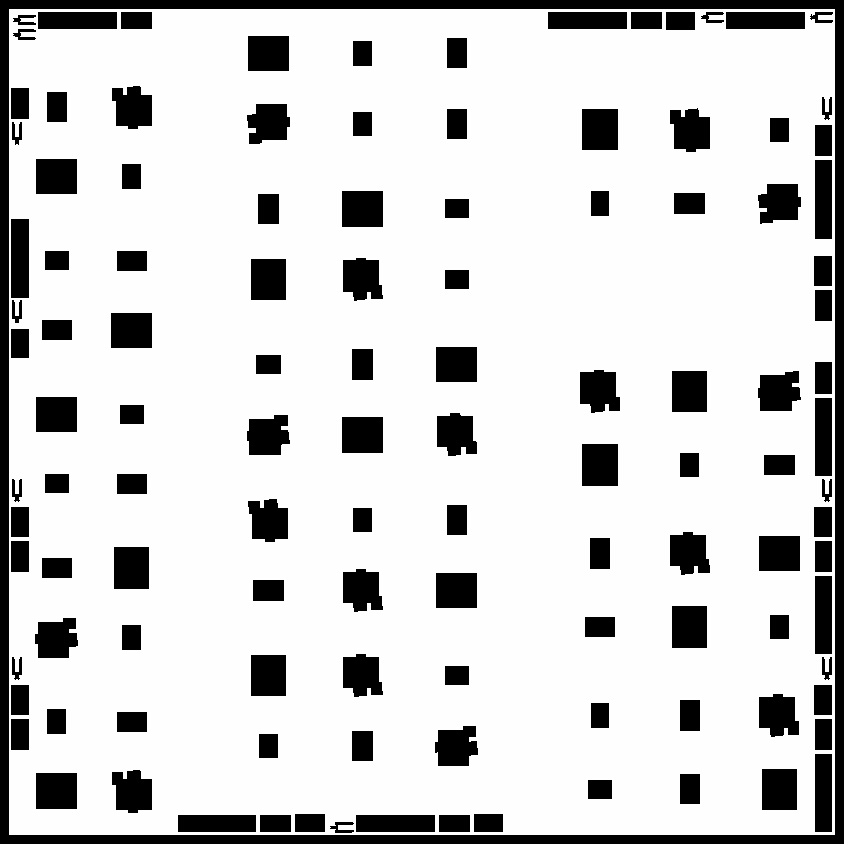
\includegraphics[width=\textwidth]{figures/warehouse_static_01.png}\\[0.4ex]
    {\footnotesize (a) static \texttt{\_01}, distributed}
  \end{minipage}\hfill
  \begin{minipage}[t]{0.32\textwidth}
    \centering
    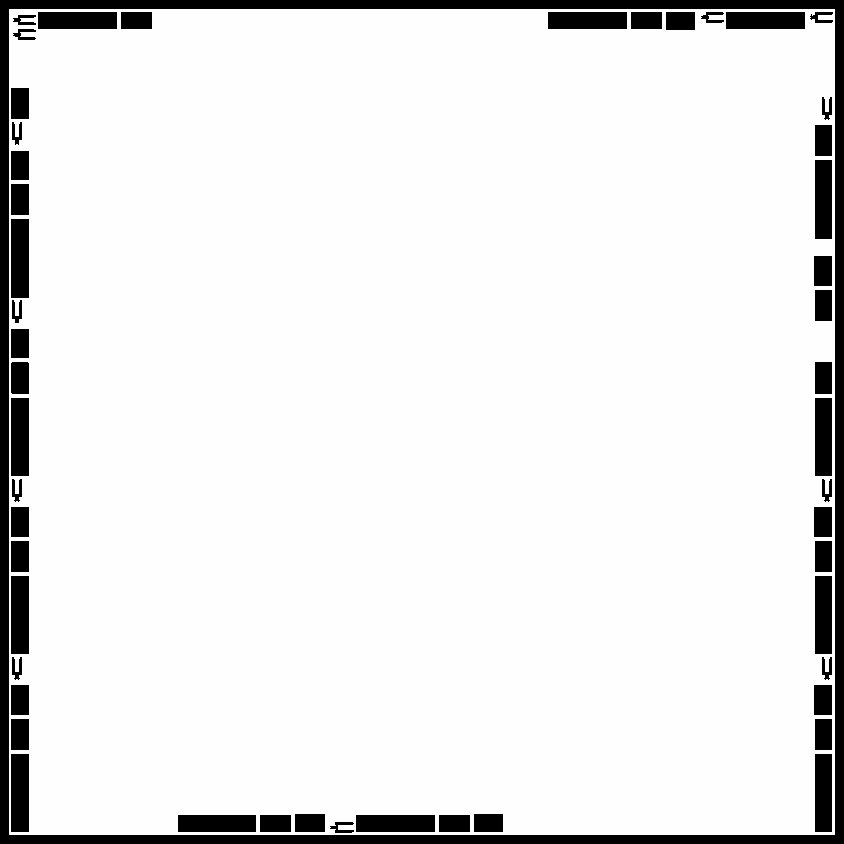
\includegraphics[width=\textwidth]{figures/warehouse_objonwallonly.png}\\[0.4ex]
    {\footnotesize (b) \texttt{objonwallonly}}
  \end{minipage}\hfill
  \begin{minipage}[t]{0.32\textwidth}
    \centering
    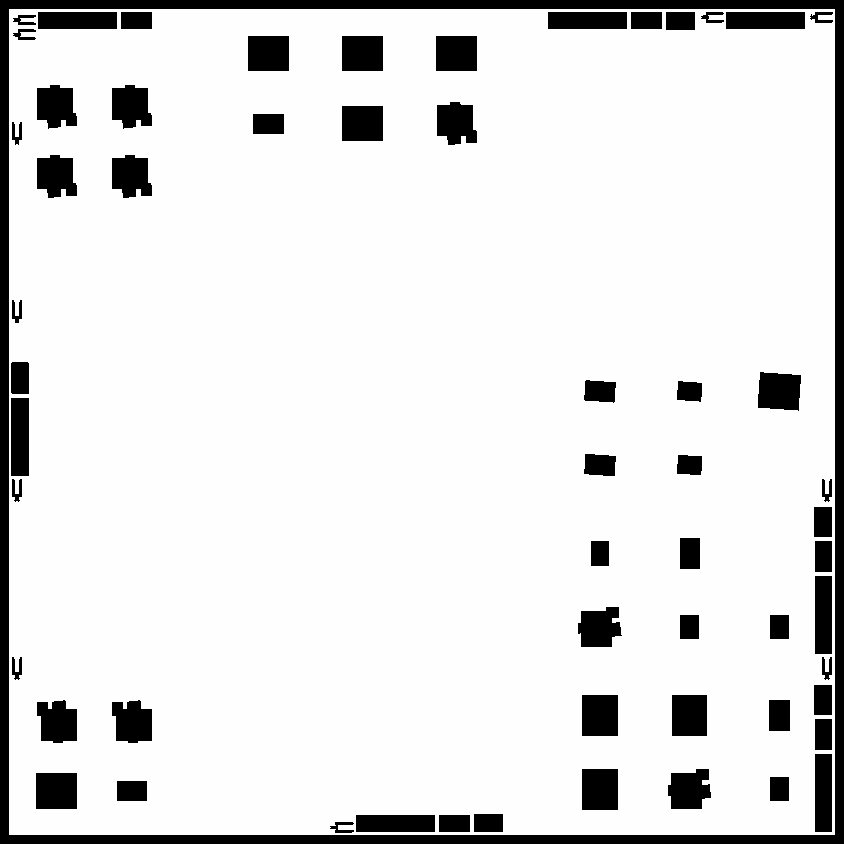
\includegraphics[width=\textwidth]{figures/warehouse_dynamic.png}\\[0.4ex]
    {\footnotesize (c) dynamic}
  \end{minipage}
  \caption[Baked occupancy truth of the three large-warehouse object arrangements, each \SI{42.2}{\metre} square at \SI{0.05}{\metre} per cell with origin $(-21.1,-21.1)$~m.]{Baked occupancy truth of the three large-warehouse object arrangements,
  each \SI{42.2}{\metre} square at \SI{0.05}{\metre} per cell with origin
  $(-21.1,-21.1)$~m. Black is occupied, white is free; there is no unknown space
  because the grids are rasterised from collision geometry rather than observed.
  Occupied cells are \SI{17.79}{\percent} of~(a), \SI{8.74}{\percent} of~(b) and
  \SI{10.98}{\percent} of~(c). Panel~(b) clears the central floor and keeps
  obstacles against the walls, which is the arrangement used by
  \repo{dataset_allsensor_002} and \repo{dataset_allsensor_003}. \emph{No
  occupancy grid is shown per floor treatment, and none exists:} the
  \texttt{bayline} and plain floors differ only in surface material, which carries
  no collision geometry, so their baked grids are identical to the panels above.
  See \cref{fig:floor-treatments}.}
  \label{fig:warehouse-maps}
\end{figure}

The floor treatment is a separate factor and is invisible to occupancy. It is set
by which ground model a world includes; those models share one mesh and differ only
in the visual materials attached to it (\cref{tab:floor-variants}).
\Cref{fig:floor-treatments} renders both recorded conditions at true scale using
\repo{script/render_floor.py}, which drives the 2-D viewer's own floor rasteriser
so that the figure shows what the overlay and the simulated cameras see rather
than a texture file out of context.

\begin{figure}[htbp]
  \centering
  \begin{minipage}[t]{0.33\textwidth}
    \centering
    
\includegraphics[width=\textwidth]{figures/floor_plain.png}\\[0.4ex]
    {\footnotesize (a) plain, \repo{allsensor_000}--\repo{_002}}
  \end{minipage}\hfill
  \begin{minipage}[t]{0.33\textwidth}
    \centering
    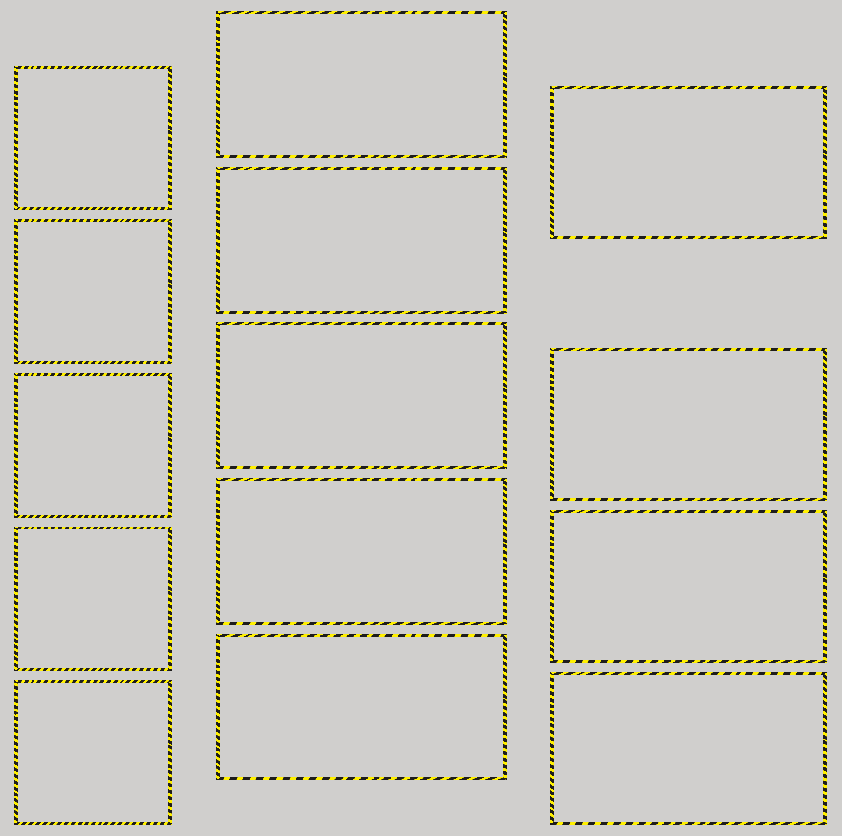
\includegraphics[width=\textwidth]{figures/floor_bayline.png}\\[0.4ex]
    {\footnotesize (b) \texttt{bayline}, \repo{allsensor_003}, \repo{_004}}
  \end{minipage}\hfill
  \begin{minipage}[t]{0.29\textwidth}
    \centering
    
\includegraphics[width=\textwidth]{figures/floor_bayline_detail.png}\\[0.4ex]
    {\footnotesize (c) \SI{12}{\metre} detail of~(b)}
  \end{minipage}
  \caption[The two recorded floor conditions, rendered across the full \SI{42.2}{\metre} floor at \SI{0.05}{\metre} per pixel.]{The two recorded floor conditions, rendered across the full
  \SI{42.2}{\metre} floor at \SI{0.05}{\metre} per pixel. Both share the same flat
  diffuse base, RGB $(0.814,0.811,0.804)$; the only difference between them is the
  112 painted marking faces that \texttt{bayline} adds, forming the hazard-striped
  outlines of fourteen storage bays. Panel~(c) is a \SI{12}{\metre} square detail
  showing the strips at \SI{0.145}{\metre} width. Everything not outlined is
  untextured in both conditions.}
  \label{fig:floor-treatments}
\end{figure}

\begin{table}[htbp]
\centering
\caption[Ground models and the floor conditions they produce.]{Ground models and the floor conditions they produce. The mesh and its
collision geometry are identical in all three, so the floor treatment changes what
a camera sees and nothing a wheel, an occupancy grid or a collision check responds
to. The concrete-grain texture belongs to the stock model only, and no recorded
dataset uses it.}
\label{tab:floor-variants}
\small
\begin{tabularx}{\textwidth}{>{\raggedright\arraybackslash}p{0.29\textwidth}lll>{\raggedright\arraybackslash}X}
\toprule
Ground model & Base & Concrete & Markings & Used by \\
\midrule
\repo{..._GroundB_01} (stock) & texture & yes & 112 faces & no recorded dataset \\
\repo{..._GroundB_01_bayline} & flat diffuse & no & 112 faces &
  \repo{allsensor_003}, \repo{allsensor_004} \\
\repo{..._GroundB_01_plain} & flat diffuse & no & none &
  \repo{allsensor_000}--\repo{_002}, all \texttt{nofloortexture} datasets \\
\bottomrule
\end{tabularx}
\end{table}

\begin{queried}[Naming]
The factor recorded in this project as ``textured versus featureless floor'' is
narrower than the name suggests, and \cref{fig:floor-treatments} is the evidence.
Both conditions rest on the \emph{same flat, untextured diffuse colour}; the stock
concrete-grain texture appears in neither. The entire difference is fourteen
painted bay outlines, \SI{0.145}{\metre} wide, covering a small fraction of a
\SI{1704}{\metre\squared} floor. A robot driving an aisle sees a uniform grey
surface in both conditions for most of its path, crossing a high-contrast strip
only at a bay boundary.

Results comparing the two floors must therefore be read as \emph{bay markings
versus nothing}, not as \emph{realistic floor versus nothing}, and the near-absence
of a visual-odometry improvement between them (\cref{sec:results-proprio}) should
not be generalised to floors carrying genuine surface texture. Testing that would
require a world built on the stock \repo{GroundB_01} model, which no recorded
dataset uses.
\end{queried}

\begin{queried}[Unverified]
The dynamic world's baked grid, \cref{fig:warehouse-maps}(c), contains
\SI{38}{\percent} fewer occupied cells than the distributed static arrangement
in~(a). \repo{bake_map.py} rasterises every \texttt{<include>} in the
world file at its authored pose, so kinematically driven props should appear at
their initial positions, but this has not been confirmed for the dynamic family.
Until it is, panel~(c) must not be used as occupancy truth for scoring a
reconstructed map of a dynamic scene: the deficit may be a genuine difference in
static stocking, or it may be props missing from the bake, and those two
possibilities imply opposite corrections. The estimator results in
\cref{sec:results-proprio} are unaffected, as they use the arrangements in
panels~(a) and~(b) only.
\end{queried}

Each recorded dataset is the combination of three things that vary independently
and are easy to confuse when read off three separate artifacts: the floor
treatment, the object arrangement, and the route the robot actually drove.
\Cref{fig:dataset-scenes} draws all three together for every dataset, and
\cref{tab:dataset-scenes} gives the numbers behind the pictures. Both are produced
by \repo{script/render_dataset_scene.py}, which resolves each dataset's world from
its own run manifest rather than from its name---necessary because
\repo{dataset_static_nofloortexture_001} sits in the \texttt{\_01} arrangement
while \repo{_000} and \repo{_002} sit in the canonical one, and all three carry
\texttt{nofloortexture} in the name.

\begin{figure}[p]
  \centering
  \begin{minipage}[t]{0.235\textwidth}
    \centering
    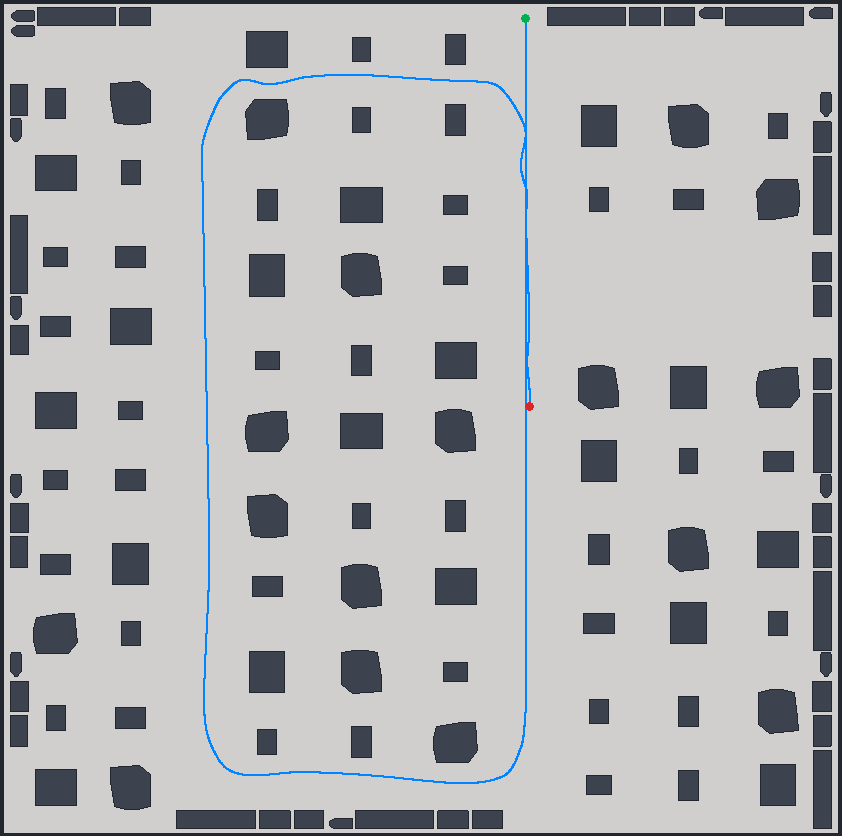
\includegraphics[width=\textwidth]{figures/scene_allsensor_000.png}\\[0.3ex]
    {\scriptsize \repo{allsensor_000}}
  \end{minipage}\hfill
  \begin{minipage}[t]{0.235\textwidth}
    \centering
    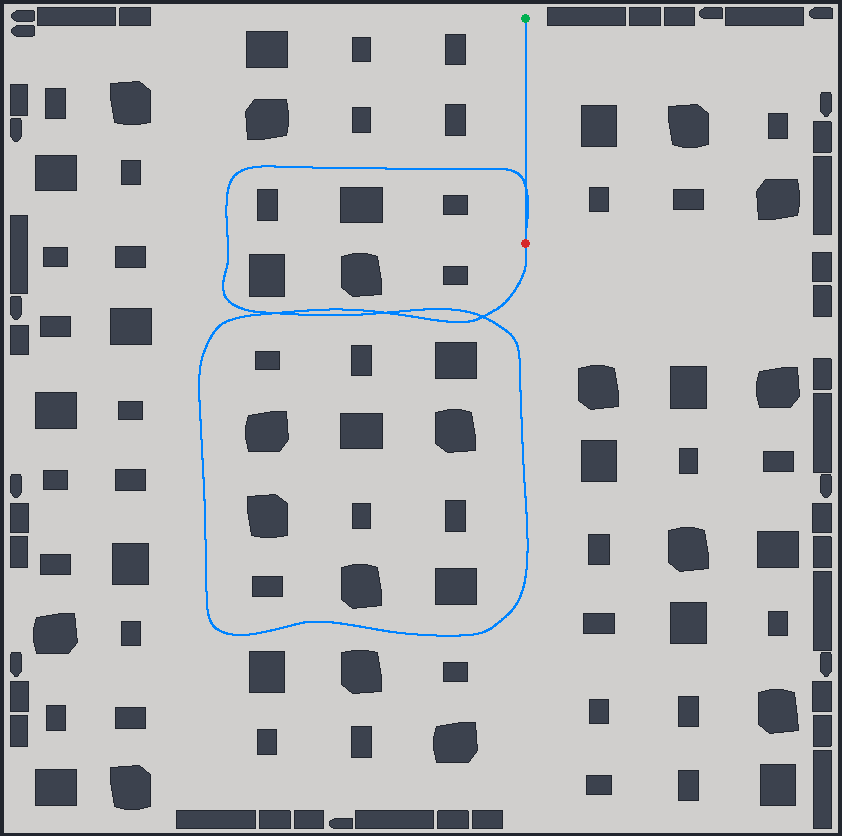
\includegraphics[width=\textwidth]{figures/scene_allsensor_001.png}\\[0.3ex]
    {\scriptsize \repo{allsensor_001}}
  \end{minipage}\hfill
  \begin{minipage}[t]{0.235\textwidth}
    \centering
    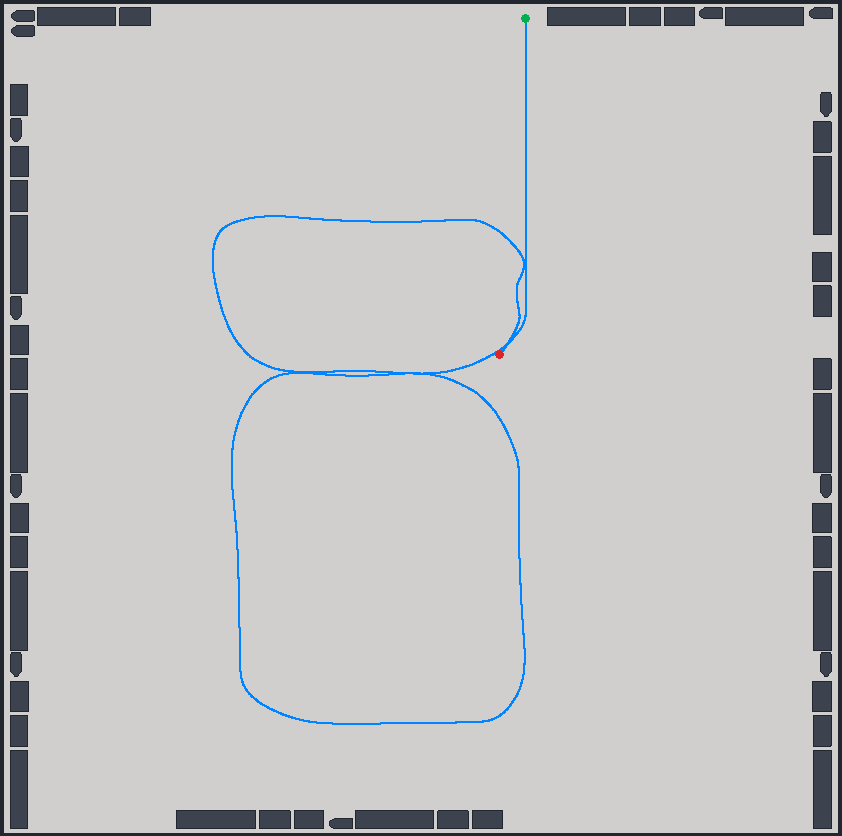
\includegraphics[width=\textwidth]{figures/scene_allsensor_002.png}\\[0.3ex]
    {\scriptsize \repo{allsensor_002}}
  \end{minipage}\hfill
  \begin{minipage}[t]{0.235\textwidth}
    \centering
    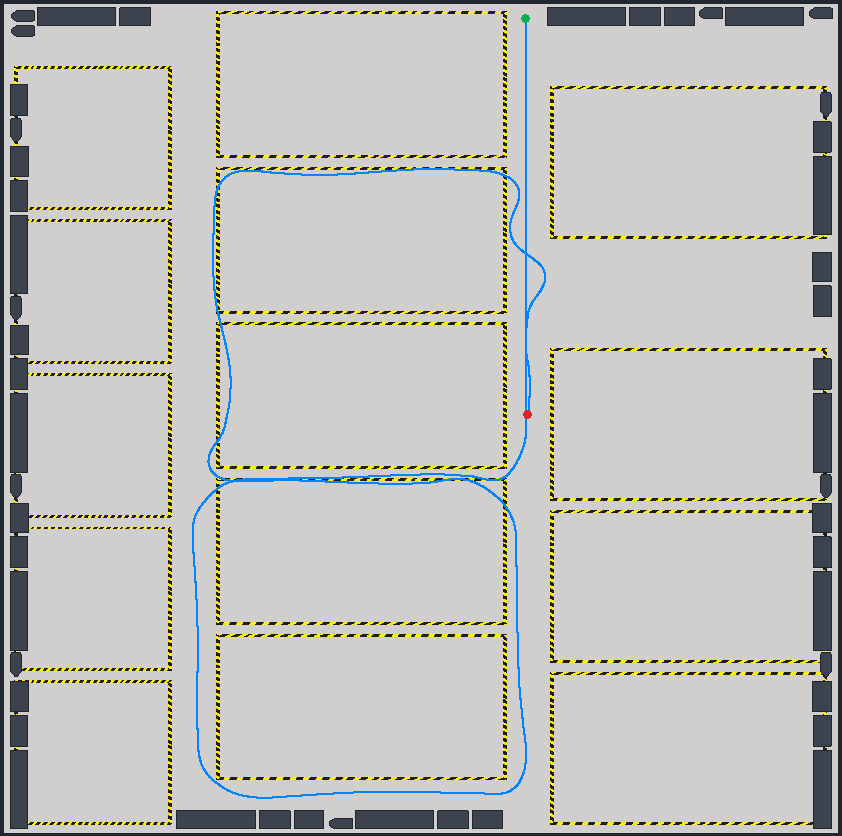
\includegraphics[width=\textwidth]{figures/scene_allsensor_003.png}\\[0.3ex]
    {\scriptsize \repo{allsensor_003}}
  \end{minipage}

  \vspace{1.2ex}
  \begin{minipage}[t]{0.235\textwidth}
    \centering
    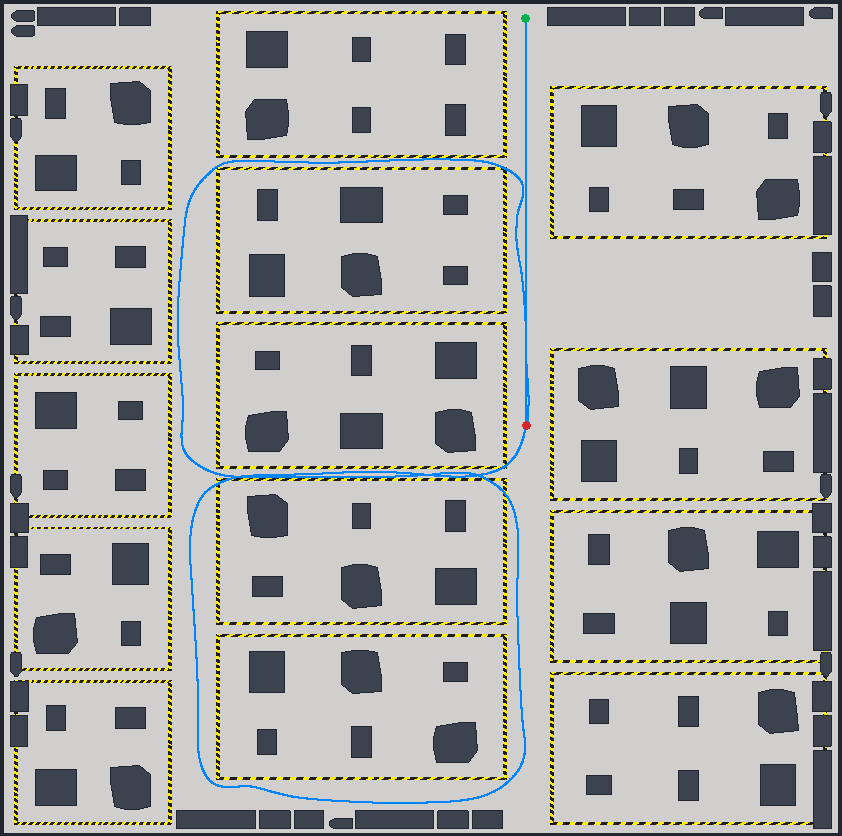
\includegraphics[width=\textwidth]{figures/scene_allsensor_004.png}\\[0.3ex]
    {\scriptsize \repo{allsensor_004}}
  \end{minipage}\hfill
  \begin{minipage}[t]{0.235\textwidth}
    \centering
    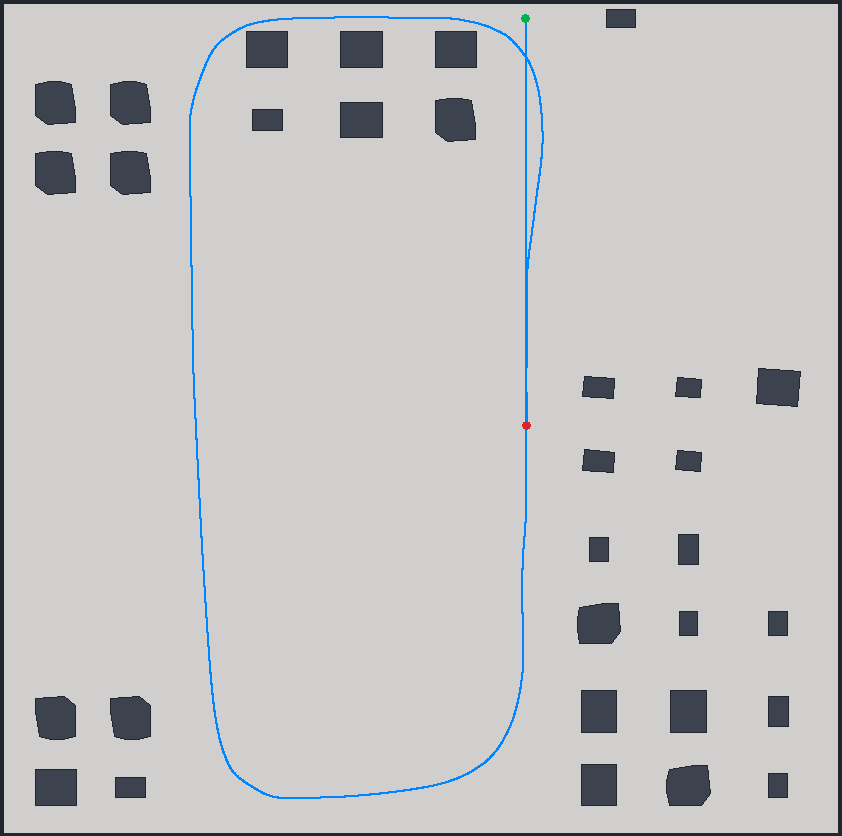
\includegraphics[width=\textwidth]{figures/scene_static_nofloortexture_000.png}\\[0.3ex]
    {\scriptsize \repo{static_000}\flag{*}}
  \end{minipage}\hfill
  \begin{minipage}[t]{0.235\textwidth}
    \centering
    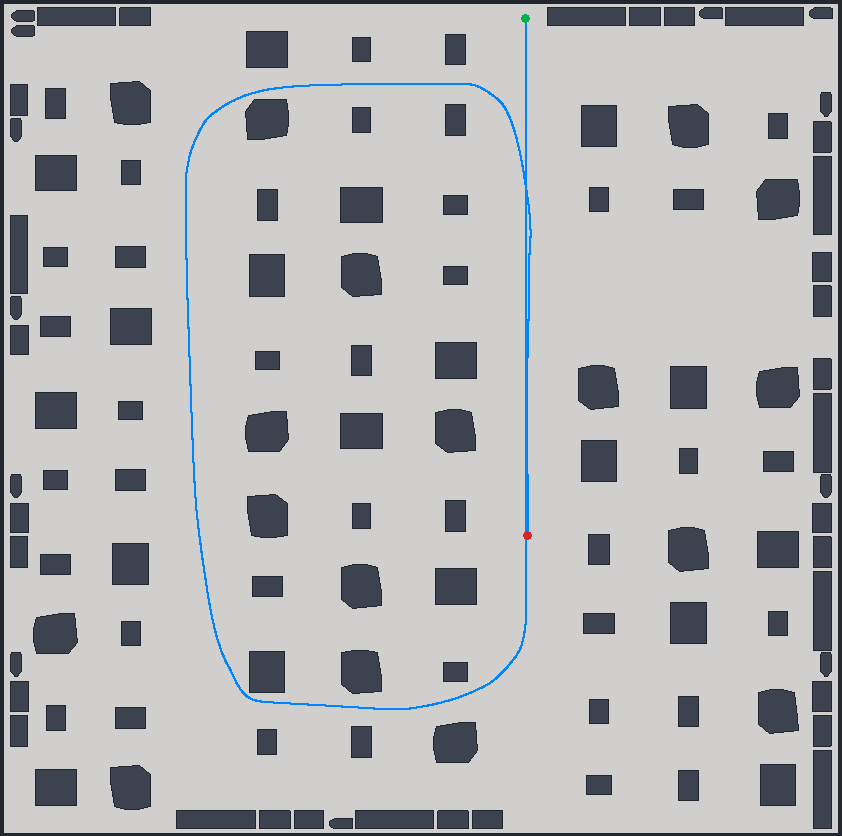
\includegraphics[width=\textwidth]{figures/scene_static_nofloortexture_001.png}\\[0.3ex]
    {\scriptsize \repo{static_001}}
  \end{minipage}\hfill
  \begin{minipage}[t]{0.235\textwidth}
    \centering
    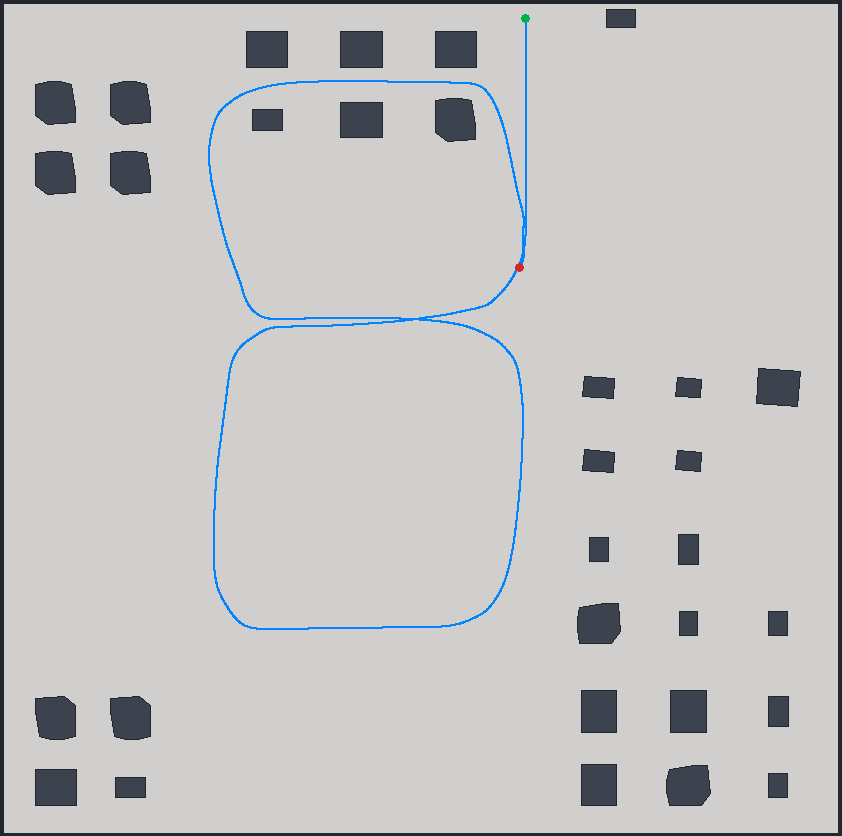
\includegraphics[width=\textwidth]{figures/scene_static_nofloortexture_002.png}\\[0.3ex]
    {\scriptsize \repo{static_002}\flag{*}}
  \end{minipage}

  \vspace{1.2ex}
  \begin{minipage}[t]{0.235\textwidth}
    \centering
    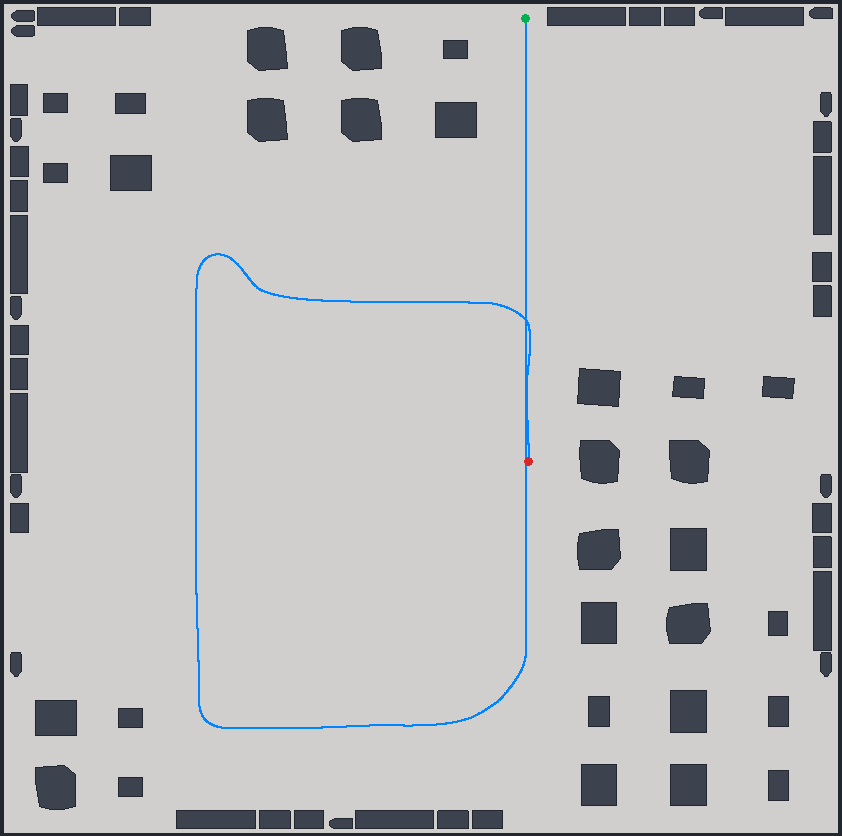
\includegraphics[width=\textwidth]{figures/scene_dynamic_nofloortexture_00_000.png}\\[0.3ex]
    {\scriptsize \repo{dynamic_00_000}}
  \end{minipage}\hfill
  \begin{minipage}[t]{0.235\textwidth}
    \centering
    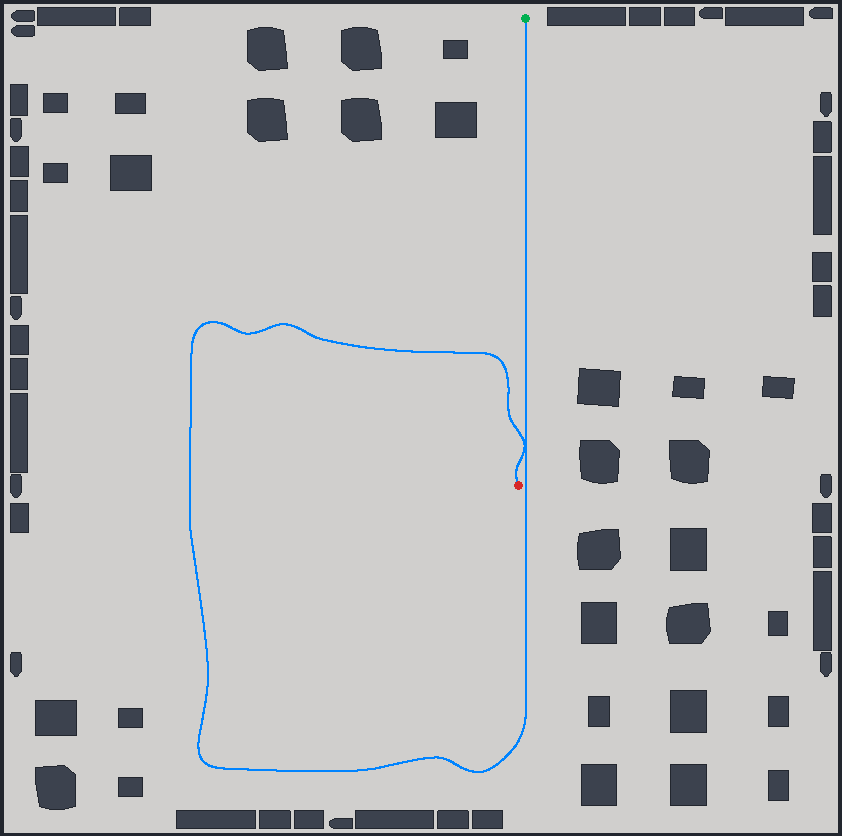
\includegraphics[width=\textwidth]{figures/scene_dynamic_nofloortexture_00_001.png}\\[0.3ex]
    {\scriptsize \repo{dynamic_00_001}}
  \end{minipage}\hfill
  \begin{minipage}[t]{0.235\textwidth}
    \centering
    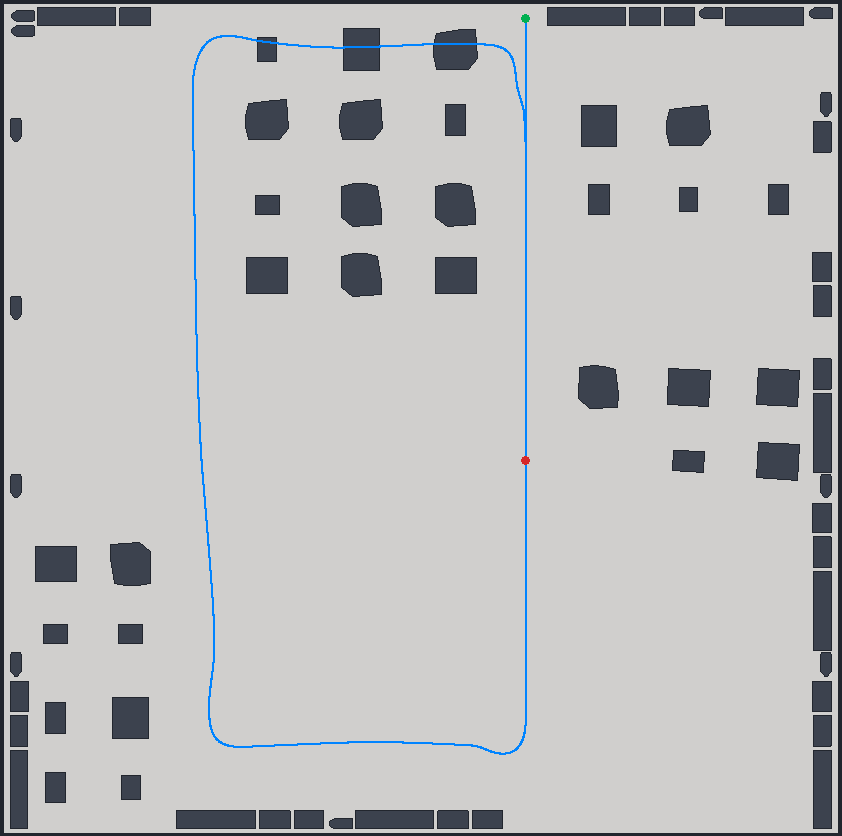
\includegraphics[width=\textwidth]{figures/scene_dynamic_nofloortexture_01_000.png}\\[0.3ex]
    {\scriptsize \repo{dynamic_01_000}}
  \end{minipage}\hfill
  \begin{minipage}[t]{0.235\textwidth}
    \centering
    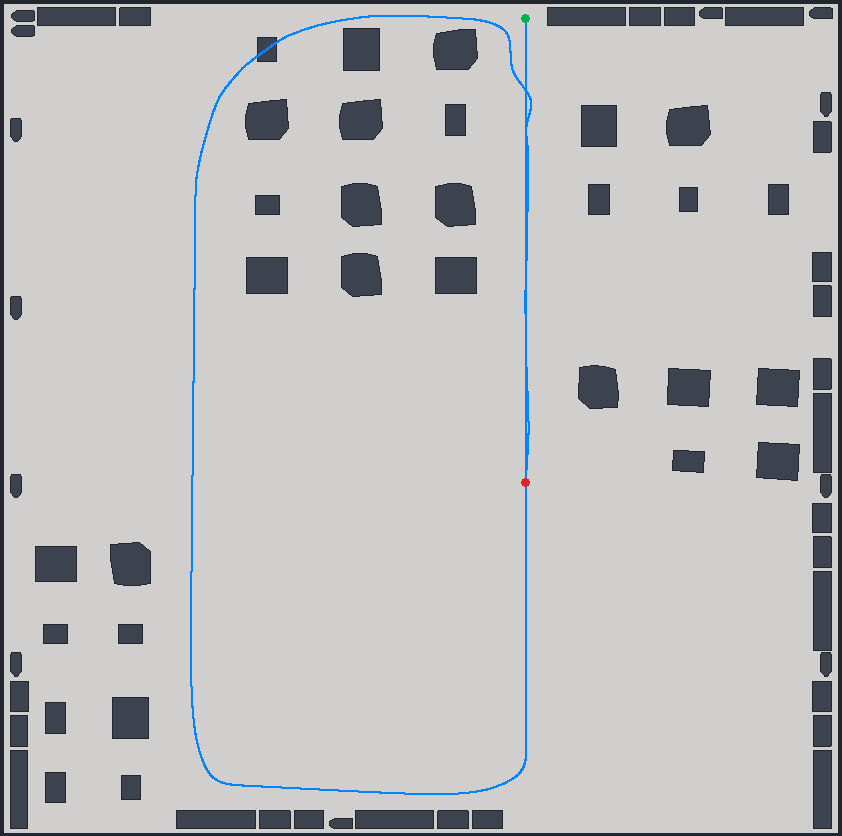
\includegraphics[width=\textwidth]{figures/scene_dynamic_nofloortexture_02_000.png}\\[0.3ex]
    {\scriptsize \repo{dynamic_02_000}}
  \end{minipage}
  \caption[Every simulation dataset as a scene: floor treatment, object layout and ground-truth route in one view.]{Every simulation dataset as a scene: floor treatment, object layout and
  ground-truth route in one view. Grey is open floor; dark polygons are obstacle
  footprints, taken as convex hulls of each collision mesh sliced at robot height,
  the same geometry the occupancy bake uses. Yellow hazard striping is the painted
  bay outline of the \texttt{bayline} floor and is absent on plain floors. The blue
  trace is the recorded \repo{/ground_truth/odometry} route, green marking its
  start and red its end. Moving props are drawn at their authored pose, which is
  where the world file places them at $t=0$; this is a layout figure and does not
  show where a prop was at any instant during a dynamic recording. \flag{*}~marks a
  dataset whose recorded world no longer exists and whose objects were
  reconstructed---see the note below \cref{tab:dataset-scenes}.}
  \label{fig:dataset-scenes}
\end{figure}

\begin{table}[htbp]
\centering
\caption[What each dataset contains.]{What each dataset contains. ``Objects'' counts obstacle instances whose
collision geometry intersects the robot-height band, excluding the wall ring.
``Route'' is the ground-truth path length and ``sim span'' its duration in
simulated time. The world column drops the floor suffix, which is given separately,
so two rows sharing a world arrangement but differing in floor are visible as such.}
\label{tab:dataset-scenes}
\footnotesize
\setlength{\tabcolsep}{3pt}
%% Generated by script/render_dataset_scene.py -- do not edit.
\begin{tabularx}{\textwidth}{>{\raggedright\arraybackslash}Xllrrrr}
\toprule
Dataset & World & Floor & Objects & Route & Sim span & Truth \\
 & arrangement & & & [\si{\metre}] & [\si{\second}] & samples \\
\midrule
\repo{dataset_allsensor_000} & \texttt{static\_01} & plain & 117 & 117.0 & 87.1 & 4354 \\
\repo{dataset_allsensor_001} & \texttt{static\_01} & plain & 117 & 113.1 & 81.8 & 4091 \\
\repo{dataset_allsensor_002} & \texttt{static\_objonwallonly} & plain & 49 & 115.2 & 86.7 & 4338 \\
\repo{dataset_allsensor_003} & \texttt{static\_objonwallonly} & bayline & 49 & 140.6 & 102.4 & 5119 \\
\repo{dataset_allsensor_004} & \texttt{static\_01} & bayline & 117 & 142.3 & 100.5 & 5026 \\
\repo{dataset_dynamic_nofloortexture_00_000} & \texttt{dynamic\_00} & plain & 69 & 97.1 & 77.4 & 3873 \\
\repo{dataset_dynamic_nofloortexture_00_001} & \texttt{dynamic\_00} & plain & 69 & 97.3 & 74.2 & 3710 \\
\repo{dataset_dynamic_nofloortexture_01_000} & \texttt{dynamic\_01} & plain & 68 & 122.8 & 84.6 & 4230 \\
\repo{dataset_dynamic_nofloortexture_02_000} & \texttt{dynamic\_02} & plain & 68 & 126.6 & 89.5 & 4475 \\
\repo{dataset_static_nofloortexture_000}\flag{*} & \texttt{static} & plain & 31 & 122.9 & 86.7 & 4334 \\
\repo{dataset_static_nofloortexture_001} & \texttt{static\_01} & plain & 117 & 113.1 & 82.0 & 4100 \\
\repo{dataset_static_nofloortexture_002}\flag{*} & \texttt{static} & plain & 31 & 114.7 & 89.5 & 4475 \\
\bottomrule
\end{tabularx}

\end{table}

\begin{queried}[Missing world]
\repo{dataset_static_nofloortexture_000} and \repo{_002} name
\repo{worlds/small_warehouse_static/small_warehouse_static_nofloortexture.world}
in their run manifests, and \flag{that file no longer exists in the repository}.
Both datasets contribute to the relogged campaign of \cref{sec:results-validity},
so their scenes could not be drawn from the recorded world and their conditions
cannot be re-inspected directly.

The panels marked \flag{*} are reconstructions. They are exact for geometry rather
than approximate, because \repo{script/make_plain_floor.py} produces a floor
variant by swapping only the ground model's \texttt{<include>} URI and leaves every
object untouched: the missing world therefore differed from the surviving
\repo{small_warehouse_static.world} in its floor alone, and that floor is
recoverable from the suffix. It remains a reconstruction and not the recorded file,
and the two datasets should be re-recorded, or the world restored from history,
before either is used for anything the floor or the object layout bears on.
\end{queried}

The available controlled factors are summarised in \cref{tab:controlled-factors}.

\begin{table}[htbp]
\centering
\caption[Controlled experimental factors available in the simulation environment, with the levels realised at the reporting cutoff.]{Controlled experimental factors available in the simulation environment,
with the levels realised at the reporting cutoff. A factor is listed as exercised
only where a recorded dataset exists for more than one of its levels.}
\label{tab:controlled-factors}
\small
\begin{tabularx}{\textwidth}{>{\raggedright\arraybackslash}p{0.21\textwidth}>{\raggedright\arraybackslash}p{0.30\textwidth}>{\raggedright\arraybackslash}X}
\toprule
Factor & Levels & Status at cutoff \\
\midrule
Scene dynamics & static props; scripted dynamic props & exercised \\
Floor markings & bay outlines present (\texttt{bayline});
  absent (plain) & exercised; no dataset carries surface texture \\
Prop or route arrangement & canonical; \texttt{\_00}; \texttt{\_01};
  \texttt{\_02} & exercised \\
Stocking level & partial; fully stocked static & fully stocked recorded \\
Object placement & distributed; restricted to the wall region & exercised, three
  bags to one \\
Domain & simulation; real robot & exercised, no real ground truth \\
World scale & tiny \repo{small_warehouse}; large rescaled families & distinct
  environments, never pooled \\
\bottomrule
\end{tabularx}
\end{table}

The plain floor removes the painted bay outlines; neither recorded condition
carries the stock concrete texture. Collision geometry and occupancy truth are
preserved in both (\cref{tab:floor-variants}). Dynamic props follow
deterministic routes through a kinematic Gazebo plugin. This preserves repeatable
motion and acceptable real-time factor, but it does not reproduce physical
collision response if the robot overlaps a moving prop.

World identity is recorded by exact \texttt{.world} path. ROS launches require
\repo{colcon build --symlink-install}; a plain build can leave an obsolete copied
world in \repo{install/}. When object motion is required by the 2-D viewer, model
poses must also be bridged from the simulator.


\subsection{Dataset registry}
\label{sec:dataset-registry}
% Verbatim from minor_report/chapters/chapter_3_methodology.tex lines 910-1043 (retired report),
% headings demoted by 0 level(s). Do not edit here; edit the source of the numbers.

Datasets are held in two places and the registry must cover both: the workspace
tree \repo{dataset/} and a removable drive mounted at
\repo{/media/ambushee/32E4AAB1E4AA772F/}, whose simulation bags sit under
\repo{dataset/} and whose real-robot recordings sit at its root.
\Cref{tab:dataset-registry} lists all eighteen recordings across both locations.
Six exist in one place only on the drive, seven in the workspace only, and three
are held in both.

\begin{sidewaystable}[p]
\centering
\caption[Complete dataset registry at the reporting cutoff, across both storage locations.]{Complete dataset registry at the reporting cutoff, across both storage
locations. The \texttt{bayline} families carry a textured floor; every other
simulation entry is featureless. ``WS'' is the workspace tree \repo{dataset/} and ``FD'' the removable
drive; a size is given where that location holds a copy. ``Prop.'' marks the
proprioceptive group (\repo{/model/ackermann_robot_001/joint_state} and
\repo{/model/ackermann_robot_001/odometry}); ``IMU'' counts inertial messages,
on \repo{/imu} for simulation and \repo{/hwt101ct_yaw_publisher} for the real
rig. Durations are rosbag wall-clock recording durations: the simulator ran below
real time, so a bag's sim-time span is shorter than the figure shown. Integrity
was checked by opening each SQLite store and counting rows against the count its
\repo{metadata.yaml} declares, not by trusting the metadata.}
\label{tab:dataset-registry}
\scriptsize
\setlength{\tabcolsep}{4pt}
\begin{tabular}{llrrrrcccl}
\toprule
Dataset & Family & WS & FD & Dur.\ (s) & Messages & \texttt{/clock} & Truth &
  Prop. & Integrity \\
 & & (MB) & (MB) & & & & & & \\
\midrule
\repo{dataset_allsensor_000} & static \texttt{\_01} & 689 & -- & 129.3 & 211\,811 &
  \checkmark & \checkmark & \checkmark & ok \\
\repo{dataset_allsensor_001} & static \texttt{\_01} & 674 & -- & 126.2 & 198\,873 &
  \checkmark & \checkmark & \checkmark & ok \\
\repo{dataset_allsensor_002} & static, wall only & 750 & -- & 105.5 & 215\,528 &
  \checkmark & \checkmark & \checkmark & ok \\
\repo{dataset_allsensor_003} & bayline, wall only & 1056 & -- & 141.2 & 255\,699 &
  \checkmark & \checkmark & \checkmark & ok \\
\repo{dataset_allsensor_004} & bayline, distributed & 1311 & -- & 168.6 & 253\,942 &
  \checkmark & \checkmark & \checkmark & ok \\
\midrule
\repo{dataset_static_nofloortexture_000} & static & -- & 592 & 101.5 & 118\,597 &
  \checkmark & \checkmark & -- & ok \\
\repo{dataset_static_nofloortexture_001} & static & 617 & 1 & 92.0 & 113\,332 &
  \checkmark & \checkmark & -- & \flag{FD stub, WS ok} \\
\repo{dataset_static_nofloortexture_002} & static & -- & 688 & 103.3 & 122\,386 &
  \checkmark & \checkmark & -- & ok \\
\repo{dataset_static_nofloortexture_objonwallonly} & static, wall only & 648 & -- &
  110.5 & 114\,523 & \checkmark & \checkmark & -- & ok \\
\midrule
\repo{dataset_dynamic_nofloortexture_00_000} & dynamic \texttt{\_00} & -- & 653 &
  100.3 & 111\,988 & \checkmark & \checkmark & -- & ok \\
\repo{dataset_dynamic_nofloortexture_00_001} & dynamic \texttt{\_00} & -- & 778 &
  167.7 & 114\,169 & \checkmark & \checkmark & -- & ok \\
\repo{dataset_dynamic_nofloortexture_01_000} & dynamic \texttt{\_01} & 713 & 710 &
  165.4 & 126\,790 & \checkmark & \checkmark & -- & \flag{FD malformed, WS ok} \\
\repo{dataset_dynamic_nofloortexture_02_000} & dynamic \texttt{\_02} & -- & 758 &
  172.1 & 134\,995 & \checkmark & \checkmark & -- & ok \\
\midrule
\repo{dataset_map_01} & mapping, large & 818 & -- & 193.5 & 152\,291 & \checkmark &
  \checkmark & -- & ok \\
\repo{dataset_map_tiny} & mapping, tiny world & 726 & -- & 63.3 & 82\,555 &
  \checkmark & \checkmark & -- & ok \\
\midrule
\repo{dataset_real_000} & real rig & 2964 & 2964 & 116.6 & 36\,166 & -- & -- & -- &
  ok, 23\,257 IMU \\
\repo{dataset_real_001} & real rig & -- & 2099 & 85.5 & 9\,629 & -- & -- & -- &
  \flag{0 IMU messages} \\
\repo{dataset_real_002} & real rig & -- & 2869 & 113.5 & 12\,682 & -- & -- & -- &
  \flag{0 IMU messages} \\
\bottomrule
\end{tabular}
\end{sidewaystable}

The seven featureless-floor simulation bags of the relogged campaign
(\cref{sec:results-validity}) are the static and dynamic families listed above;
five were read from the drive and two from the workspace, for the reason recorded
next.

\begin{queried}[Data integrity]
Two drive copies are unreadable while presenting a complete, plausible
\repo{metadata.yaml}. \repo{dataset_static_nofloortexture_001} is a
\SI{524288}{\byte} stub whose metadata nevertheless declares 113\,332 messages,
and \repo{dataset_dynamic_nofloortexture_01_000} is \SI{710}{\mega\byte}---within
\SI{0.4}{\percent} of its workspace counterpart---with a valid SQLite header but a
store that reports \emph{database disk image is malformed} on any query. Both have
intact workspace copies, which is why those two datasets were read from the
workspace in the relogged campaign.

The general lesson is recorded as a control rather than an incident:
\repo{metadata.yaml} is written when recording begins and does not describe what
survived, so message counts, durations and topic lists copied from it are not
evidence that a bag is intact. Storage health must be established by opening the
SQLite store and counting rows, which is now part of the pre-experiment inspection
in \cref{sec:collection-validity}.
\end{queried}

\begin{queried}[Scope limit]
Only the five \repo{dataset_allsensor} bags carry wheel encoders and wheel
odometry; the other thirteen recordings omit those topics entirely. The
proprioceptive baseline of \cref{sec:results-proprio} therefore cannot be computed
for any dynamic condition, for the mapping bags, or for the real rig, and the
comparison between proprioception and visual odometry exists only in
\emph{static, featureless-floor} scenes---the conditions least favourable to
vision and most favourable to dead reckoning. Extending it requires re-recording
with the two topics bridged, not new analysis.
\end{queried}

\begin{queried}[Excluded]
\repo{dataset_real_001} and \repo{dataset_real_002} are excluded because their
inertial topic \repo{/hwt101ct_yaw_publisher} contains \emph{zero} messages, so
neither supports stereo-inertial operation at all. Their image streams are intact
(2\,562 and 3\,405 pairs), so they remain usable for detector or image-only work.
\repo{dataset_real_000} is the only real recording with inertial data, at 23\,257
messages.
\end{queried}

Historical output folders do not prove that their raw bags remain available or
valid. Conversely, a dataset is not marked broken merely because its only copy
lives on the removable drive rather than in the repository; six of the fifteen
recordings are drive-only and are sound.

Before a new experiment, the bag's absolute path, topics, duration, message
counts, and storage health are inspected. Each paired comparison uses the same
recording, and estimators run separately to avoid resource-contention effects.
Environment, trajectory, calibration, replay rate, image transport,
initialization treatment, and revision are controlled. A run is excluded if
input overlap, initialization, processed sample count, or sensor delivery differs
materially from its paired condition.

Recorded simulation bags used by RTAB-Map contain \texttt{/clock}. They are
played without rosbag's additional \texttt{--clock} option because competing
clock sources cause TF time jumps. This choice is made after inspecting each bag,
not applied as a universal command rule.


\section{Real Platform}
\label{sec:real-platform}

\subsection{AMR mobile robot testbed}

The system is installed and tested on a Gensurv Robotics mobile-robot base
designed to reproduce the behaviour of an industrial warehouse AMR
(\cref{fig:amr-dimensions,fig:amr-hardware}). Its maximum speed is set to
\SI{1.5}{\metre\per\second}, the limit of the SLAM stability tests. The
drivetrain is a rear brushless motor (Flipsky 6384) through a BLDC drive with
a Dynamixel RX-64 steering servo, a GigaDevice GD32407V microcontroller on a CAN
link to the NRU-51V, an LM2596 regulator from a lithium-polymer pack, and a
Wi-Fi router for tele-operation from a smartphone.
\flag{The faculty template describes the base as a differential-drive robot;
the hardware diagram (a single traction motor with a steering servo) and the
simulated model of \cref{fig:ackermann-robot} are Ackermann. The description
here follows the hardware and should be confirmed by the author.}

\begin{figure}[htbp]
  \centering
  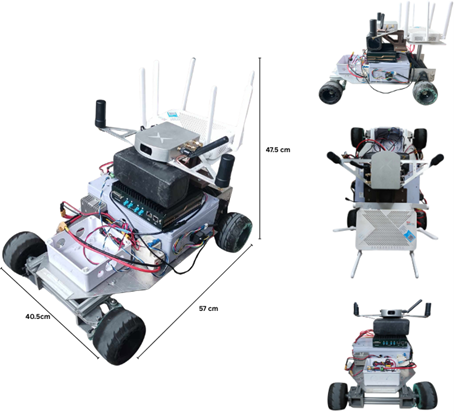
\includegraphics[width=0.75\textwidth]{figures/template/amr_dimensions.png}
  \caption{Dimensions of the mock AMR used to test the navigation system:
  \SI{57}{\centi\metre} long, \SI{40.5}{\centi\metre} wide and
  \SI{47.5}{\centi\metre} high to the top of the sensor mast.}
  \label{fig:amr-dimensions}
\end{figure}

\begin{figure}[htbp]
  \centering
  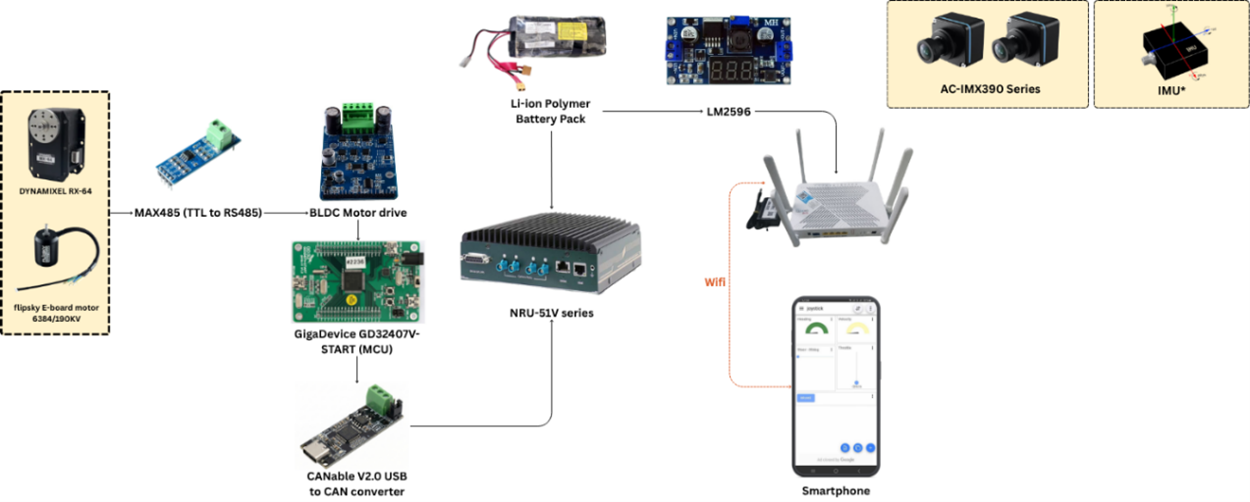
\includegraphics[width=\textwidth]{figures/template/amr_hardware.png}
  \caption[Hardware components of the mock AMR: steering servo and traction motor, BLDC drive and microcontroller on CAN, the NRU-51V computer, power supply, the AC-IMX390 stereo pair and IMU, and the Wi-Fi link to the smartphone joystick.]{Hardware components of the mock AMR: steering servo and traction
  motor, BLDC drive and microcontroller on CAN, the NRU-51V computer, power
  supply, the AC-IMX390 stereo pair and IMU, and the Wi-Fi link to the
  smartphone joystick.}
  \label{fig:amr-hardware}
\end{figure}

\subsection{Sensors and computing unit}

\textbf{Wide-angle stereo cameras (AC-IMX390-H190).} Two AC-IMX390-H190
modules form the stereo pair (\cref{fig:camera-dimensions});
\cref{tab:camera-spec} lists the specification.

\begin{figure}[htbp]
  \centering
  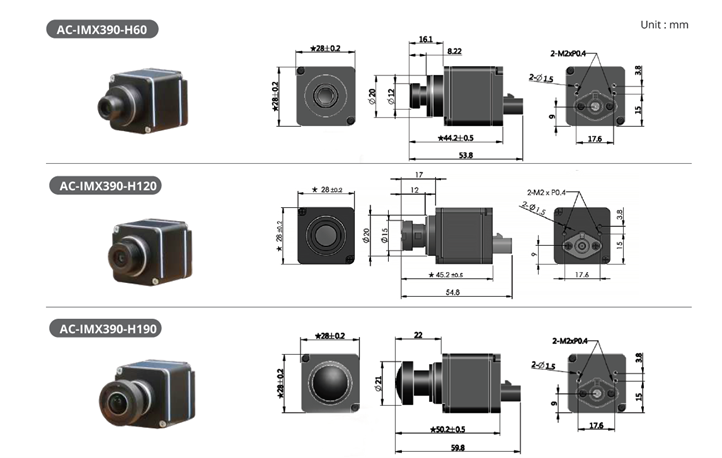
\includegraphics[width=0.9\textwidth]{figures/template/camera_dimensions.png}
  \caption{Dimensions of the AC-IMX390 camera family in millimetres; the
  H190 variant at the bottom is the one used.}
  \label{fig:camera-dimensions}
\end{figure}

\begin{table}[htbp]
\centering
\caption{Specification of the AC-IMX390-H190 camera.}
\label{tab:camera-spec}
\small
\begin{tabularx}{\textwidth}{>{\raggedright\arraybackslash}p{0.30\textwidth}>{\raggedright\arraybackslash}X}
\toprule
Item & Detail \\
\midrule
Sensor and ISP & Sony IMX390 CMOS sensor with GEO Semiconductor GW5200 ISP \\
Resolution and frame rate & $1920\times1080$ (2\,MP) at \SI{30}{fps} \\
Horizontal field of view & \SI{186}{\degree} \\
Video output & uncompressed YUV422 (UYVY) \\
Dynamic range & \SI{120}{\decibel} high dynamic range (HDR) \\
Special features & LED flicker mitigation (LFM), 5-axis active alignment \\
Environmental rating & IP67 and IP69K (lens side) \\
Operating temperature & \SIrange{-40}{85}{\celsius} \\
Connector & male FAKRA \\
\bottomrule
\end{tabularx}
\end{table}

\textbf{Inertial measurement unit.} A six-axis IMU measures linear acceleration
and angular rate at \SIrange{100}{200}{\hertz}. Its data enter IMU
pre-integration and are fused with the camera images to support the odometry
estimate while the camera moves fast or the image is momentarily blurred. On
the recorded real datasets the inertial stream is the
\repo{/hwt101ct_yaw_publisher} topic (\cref{tab:real-rig}).

\textbf{Edge AI computing unit: Neousys NRU-51V (NVIDIA Jetson Xavier NX).}
To run the deep-learning model (YOLO26) and the visual-inertial SLAM on the
robot without a central computer, the project uses the Neousys NRU-51V, a
compact industrial edge computer designed for vision and autonomous-vehicle
systems (\cref{fig:nru51v-photo,fig:nru51v-dimensions}).
\Cref{tab:hardware-spec} summarises the hardware.

\begin{figure}[htbp]
  \centering
  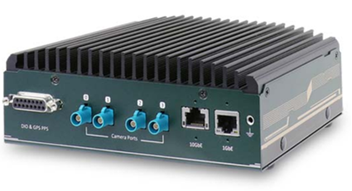
\includegraphics[width=0.55\textwidth]{figures/template/nru51v_photo.png}
  \caption{The Neousys NRU-51V (NVIDIA Jetson Xavier NX), showing the four
  FAKRA camera ports.}
  \label{fig:nru51v-photo}
\end{figure}

\begin{figure}[htbp]
  \centering
  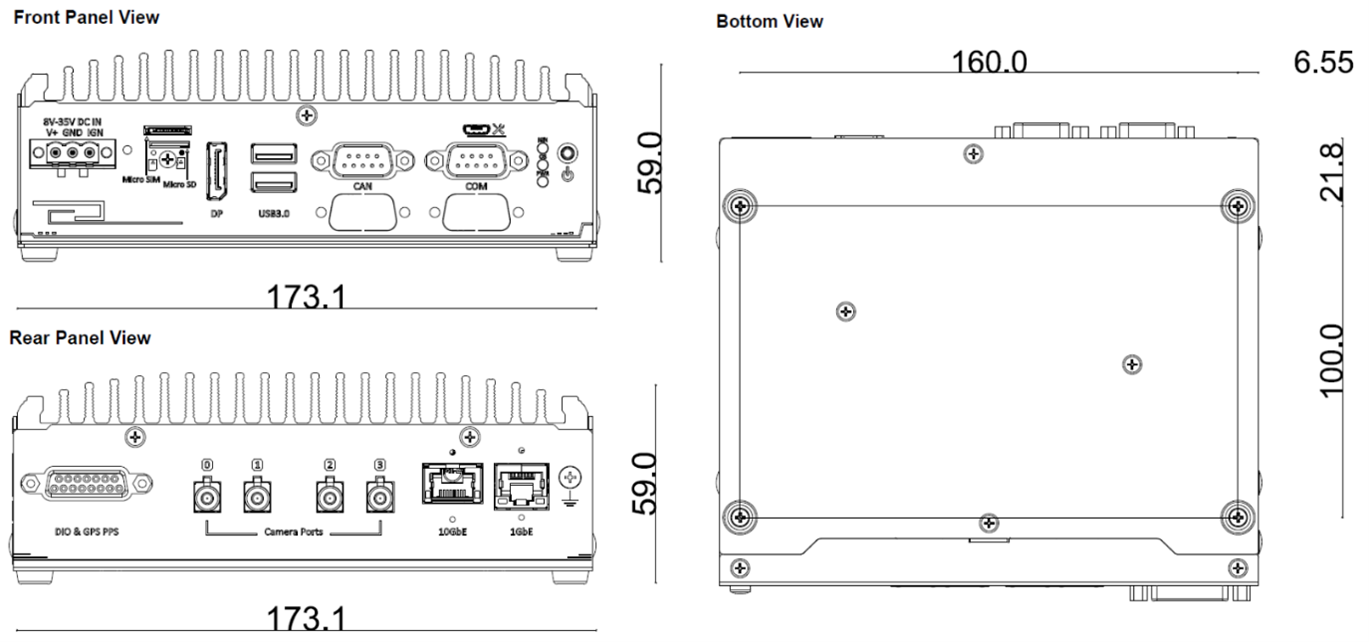
\includegraphics[width=\textwidth]{figures/template/nru51v_dimensions.png}
  \caption{Dimensions of the Neousys NRU-51V in millimetres.}
  \label{fig:nru51v-dimensions}
\end{figure}

\begin{table}[htbp]
\centering
\caption{Summary of the hardware technical specification.}
\label{tab:hardware-spec}
\small
\begin{tabularx}{\textwidth}{>{\raggedright\arraybackslash}p{0.22\textwidth}>{\raggedright\arraybackslash}p{0.34\textwidth}>{\raggedright\arraybackslash}X}
\toprule
Device / sensor & Model / specification & Role in the system \\
\midrule
Edge processing unit & Neousys NRU-51V (NVIDIA Jetson Xavier NX, 21~TOPS) &
  runs YOLO26, the SLAM system and the ROS~2 navigation stack \\
Stereo camera module & AC-IMX390-H190 (Sony IMX390 sensor) & records
  \SI{186}{\degree} stereo imagery for object detection and feature
  extraction \\
Inertial sensor (IMU) & 6-DoF industrial IMU (\SIrange{100}{200}{\hertz}) &
  measures acceleration and angular rate to support pose estimation (VIO) \\
Mobile testbed & AMR platform (speed \SI{1.5}{\metre\per\second}, slope
  \SI{5}{\degree}) & robot base for online navigation tests in the mock
  environment \\
\bottomrule
\end{tabularx}
\end{table}

\subsection{Real sensor rig and calibration limits}
\label{sec:real-calibration}
% Verbatim from minor_report/chapters/chapter_3_methodology.tex lines 534-573 (retired report),
% headings demoted by 0 level(s). Do not edit here; edit the source of the numbers.

The real configuration is summarised in \cref{tab:real-rig}. Its calibration is
materially weaker than the simulated rig's, and the weaknesses are load bearing
rather than cosmetic.

\begin{table}[htbp]
\centering
\caption[Real sensor rig, and the calibration status of each quantity.]{Real sensor rig, and the calibration status of each quantity. Only the
first three rows are measured; the remainder are approximations or placeholders
that bound what can be claimed from real-robot data.}
\label{tab:real-rig}
\small
\begin{tabularx}{\textwidth}{>{\raggedright\arraybackslash}p{0.26\textwidth}>{\raggedright\arraybackslash}p{0.30\textwidth}>{\raggedright\arraybackslash}X}
\toprule
Quantity & Value & Status \\
\midrule
Stereo resolution & $1920\times1080$ fisheye & measured \\
Stereo baseline & \SI{0.093604}{\metre} & measured \\
IMU stream & \repo{/hwt101ct_yaw_publisher} & separate RealSense source \\
Camera model (ORB-SLAM3) & \texttt{KannalaBrandt8} & configured \\
Camera model (VINS) & project fisheye files & configured \\
Second-camera intrinsics & reuse of the first camera & \flag{approximation} \\
IMU-to-camera rotation & observational support & partial \\
IMU-to-camera translation & zero & \flag{placeholder} \\
Stationary $\lVert a\rVert$ & \SI{9.2642}{\metre\per\second\squared} &
  \flag{measured, deviates from \num{9.81}} \\
Extrinsic estimation (VINS) & \repo{estimate_extrinsic: 1} & online \\
Time-offset estimation (VINS) & \repo{estimate_td: 1} & online \\
\bottomrule
\end{tabularx}
\end{table}

The real IMU-to-camera rotation has observational support, but its translation is
a zero placeholder. The stationary accelerometer magnitude is recorded as
\SI{9.2642}{\metre\per\second\squared}, rather than
\SI{9.81}{\metre\per\second\squared}. VINS-Fusion uses the observed magnitude as
\repo{g_norm}; the ORB-SLAM3 real inertial launch rescales acceleration by
$9.81/9.2642$. These treatments make the configurations internally consistent but
do not replace an independent camera--IMU calibration. Real trajectories can be
inspected for plausibility and tracking continuity, but metric accuracy cannot be
claimed without independent ground truth and improved extrinsic calibration.


\subsection{Test site and experimental variables}
\label{sec:real-site}

\textbf{Spatial layout.} The test area is divided into two operating zones,
Zone~A and Zone~B, separated by and connected through a walkway (each zone
about \SI{3}{\metre} square, walkway \SI{1.25}{\metre} wide;
\cref{fig:test-field}). The division reproduces the traffic pattern of a
warehouse AMR that shuttles continuously between a pick-up and a drop-off
point. The robot's linear speed is limited to $v_{\max} =
\SI{1.5}{\metre\per\second}$ throughout.

\textbf{Ground truth by motion capture.} Evaluating SLAM error (ATE and RPE)
needs a reference accurate to millimetres. A motion-capture camera system is
installed around the test area and tracks reflective markers placed at the
robot's centre of mass at a rate above \SI{100}{\hertz}.

\textbf{Coordinate-frame alignment.} The SLAM pose $P_{\mathrm{slam}}$ is
expressed in the local odometry frame fixed at start-up, whereas the
motion-capture pose $P_{\mathrm{gt}}$ is expressed in the room's global frame.
Before errors are computed the two trajectories are aligned by a rigid-body
transformation; the alignment actually used for every result in this report,
and its treatment of scale, is defined in \cref{sec:method-trajectory}.

\textbf{Dynamic-environment variable.} Each time the robot completes a zone
transfer (for example arrives in Zone~B from Zone~A), the operator randomly
re-positions and re-counts the stacks of goods in the opposite zone before the
robot returns. This forces the SLAM system to face a scene that no longer
matches its map (map obsolescence), to test whether ORB-SLAM3's Atlas or
RTAB-Map's memory management can resolve the conflicting spatial evidence
without tracking loss.

\textbf{Illumination variable.} Data are collected along the same route at
three times of day representing different light levels and directions:
morning (08:00), oblique natural light casting shadows across the test area;
midday (12:00), maximum brightness, with possible high contrast or
over-exposure in places; and evening (18:00), low light relying mainly on the
building's artificial lighting, with raised image noise. The variable tests
both the camera hardware (Sony IMX390 HDR) and the robustness of the two SLAM
frameworks in keeping enough inlier features for odometry under variable light.

\textbf{Real-dataset status.} Three real recordings exist
(\cref{tab:dataset-registry}). Only \repo{dataset_real_000} carries inertial
data; \repo{dataset_real_001} and \repo{_002} contain zero IMU messages and
support image-only work at most. No real recording carries motion-capture
ground truth or wheel odometry at the cutoff, which is why every real-robot
result slot in \cref{chap:results} is planned rather than filled.

\section{The Four Experiments}
\label{sec:experiments}

Each experiment below is defined by its objective, its process, its evaluation
metrics, its constraints and the validity rule that decides whether a run
counts. Each is run in both domains; \cref{chap:results} reports each domain in
its own slot.

\subsection{Experiment 1: Non-visual baseline and estimator comparison}
\label{sec:proprio-method}

\textbf{Objective.} Establish a dead-reckoning baseline to determine whether the
visual pipelines (ORB-SLAM3 and VINS-Fusion) genuinely outperform the robot's
own wheel odometry, its IMU, and a wheel-plus-IMU extended Kalman filter, and
whether the uncertainty each estimator reports describes the error it makes.

\textbf{Process.} Wheel odometry, IMU dead reckoning and the EKF are run
offline on the same recordings the visual estimators consumed, from
proprioceptive topics only. A calibration pass measures each sensor's noise and
scale against ground truth first; the estimators then run and are scored on the
same interval as the visual runs.

\textbf{Evaluation metrics.} Aligned and anchored ATE, final drift as a fraction
of distance, final heading error, RPE at \SI{1}{\second}, and the covariance
consistency measures NEES and $k\sigma$ coverage.

\textbf{Validity rule.} A run counts only if the planar assumption holds
(maximum tilt below \SI{1}{\degree}), the IMU orientation field is not consumed,
and the number of wheel corrections equals the number of wheel-odometry
messages.

% Verbatim from minor_report/chapters/chapter_3_methodology.tex lines 1263-1478 (retired report),
% headings demoted by 1 level(s). Do not edit here; edit the source of the numbers.

The visual estimators were, until the cutoff, scored only against ground truth.
That establishes how large their error is but not whether it is good, because no
alternative was measured on the same data. Three non-visual estimators were
therefore implemented in \repo{script/proprio_estimator.py} to supply a
dead-reckoning floor: wheel odometry, IMU dead reckoning, and an extended Kalman
filter fusing the two. They consume only proprioceptive topics and no images.

\subsubsection{Implementation form and why it is offline}

All three read the recorded bag directly and are deterministic functions of it.
Run as live ROS nodes they would instead depend on replay rate, QoS delivery and
CPU contention, none of which is a property of the estimator being compared. The
cost is a stated asymmetry: the visual figures they are compared against were
produced by live runs, so any timing-induced error is present on one side of the
comparison only. This is revisited in \cref{sec:results-proprio}.

\subsubsection{Sensor model derived from data}

Every covariance field in the source bags is identically zero---0 of 17\,416 IMU
messages, 0 of 4\,355 wheel-odometry messages, and 0 of 4\,354 ground-truth
messages in \repo{dataset_allsensor_000}. Gazebo Fortress does not populate them,
and \texttt{AckermannSteering} exposes no noise parameter. The noise model is
consequently measured rather than read, by a \repo{calibrate} step that writes
\repo{sensor_noise.yaml}; \cref{tab:proprio-noise} gives the result for both bags.

\begin{table}[htbp]
\centering
\caption[Sensor noise and scale measured from each bag by \repo{proprio_estimator.py calibrate}.]{Sensor noise and scale measured from each bag by
\repo{proprio_estimator.py calibrate}. Scales are least-squares gains through the
origin against ground truth; $\sigma$ values are the residual standard deviations.
A scale of 1.0 is an unbiased sensor. The bias random walks are assumed, not
measured, because the longest stationary window is \SI{1.54}{\second}.}
\label{tab:proprio-noise}
\small
\resizebox{\textwidth}{!}{%
\begin{tabular}{llrrrrrl}
\toprule
Group & Quantity & \repo{_000} & \repo{_001} & \repo{_002} & \repo{_003} &
  \repo{_004} & Units \\
 & & plain & plain & plain & bayline & bayline & \\
\midrule
IMU & gyroscope $z$ bias & $6.48\times10^{-5}$ & $7.75\times10^{-5}$ &
  $9.28\times10^{-5}$ & $6.09\times10^{-4}$ & $2.58\times10^{-5}$ & \si{\radian\per\second} \\
 & gyroscope $\sigma$ & $4.36\times10^{-3}$ & $4.24\times10^{-3}$ &
  $4.81\times10^{-3}$ & $5.03\times10^{-3}$ & $5.15\times10^{-3}$ & \si{\radian\per\second} \\
 & gyroscope $z$ scale & 0.9990 & 1.0000 & 1.0002 & 1.0002 & 1.0000 & -- \\
 & accelerometer $x$ bias & 0.0191 & 0.0304 & \flag{0.0683} & 0.0309 & 0.0016 &
  \si{\metre\per\second\squared} \\
 & accelerometer $x$ scale & 1.0199 & 1.0249 & \flag{1.0669} & \flag{1.0525} & \flag{1.0465} & -- \\
 & measured $g$ & 9.7809 & 9.8191 & 9.7827 & 9.8037 & 9.8346 & \si{\metre\per\second\squared} \\
\midrule
Wheel & speed scale & 1.0002 & 0.9985 & 1.0005 & 1.0071 & 1.0001 & -- \\
 & speed $\sigma$ & 0.0407 & 0.0484 & 0.0496 & 0.0607 & 0.0505 & \si{\metre\per\second} \\
 & yaw-rate scale, bicycle & 1.0110 & 0.9527 & 1.0034 & \flag{0.9375} & \flag{0.9250} & -- \\
 & yaw-rate $\sigma$, bicycle & 0.0659 & 0.0804 & 0.0705 & 0.1192 & 0.0613 &
  \si{\radian\per\second} \\
 & yaw-rate scale, differential & 1.2162 & 1.1442 & 1.2194 & 1.2748 & 1.1404 & -- \\
 & yaw-rate $\sigma$, differential & 0.2359 & 0.3074 & 0.2620 & 0.3477 & 0.2828 &
  \si{\radian\per\second} \\
\midrule
Window & static duration & 0.68 & 0.58 & 1.54 & 1.04 & \flag{0.52} & \si{\second} \\
 & maximum tilt & 0.0016 & 0.0018 & 0.0015 & 0.0018 & 0.0017 & \si{\degree} \\
\bottomrule
\end{tabular}}
\end{table}

Two consequences follow directly. First, wheel \emph{speed} is essentially
unbiased on all five bags (scale 1.0002 to 1.0071), so distance travelled is not
the error source. Second, the rear-wheel differential is a far worse yaw-rate estimator
than the steering-angle bicycle model---residuals of \SIrange{0.26}{0.35}{\radian\per\second}
against \numrange{0.061}{0.119}---because the track
and the wheel base are both \SI{0.42}{\metre} and a solid rear axle slips through
every turn. The bicycle model is selected automatically and was chosen on all five
bags.

\subsubsection{The orientation field must not be used}

\texttt{sensor\_msgs/Imu.orientation} in these bags is not an estimate. Measured
over \repo{dataset_allsensor_000} it equals ground-truth yaw minus exactly
\SI{90}{\degree}, with residual standard deviation \SI{0.00000}{\degree} and
\SI{0.00000}{\degree} of drift across \SI{87}{\second}: the plugin publishes the
true orientation from the simulator's entity-component manager. Consuming it
would give a ``dead-reckoning'' estimator a perfect attitude reference that no
real IMU has, and its output would measure ground truth. All three estimators
therefore integrate \texttt{angular\_velocity.z} instead, which drifts honestly by
\SI{2.52}{\degree} over \SI{87}{\second} on \repo{allsensor_000} and
\SI{1.70}{\degree} over \SI{81.8}{\second} on \repo{allsensor_001}. The same check
on \repo{allsensor_002} again returns a residual standard deviation of
\SI{0.000000}{\degree} against ground-truth yaw, so the exclusion is not specific
to the first two recordings. Each run
records \repo{imu_orientation_used=NO} in its metadata so the exclusion is
auditable.

\subsubsection{Estimator definitions}

\Cref{tab:proprio-estimators} defines the three estimators. The EKF carries the
planar state $\mathbf{x}=[p_x,p_y,\theta,v,b_\omega]^{\top}$, predicted at the
\SI{200}{\hertz} IMU rate and corrected at \SI{50}{\hertz} by the wheels.

\begin{table}[htbp]
\centering
\caption[Implemented non-visual estimators.]{Implemented non-visual estimators. ``Anchoring'' refers to the initial
pose: dead reckoning has no global reference, so all three start from the
ground-truth pose at their first sample, and this is recorded as an alignment
decision rather than treated as neutral.}
\label{tab:proprio-estimators}
\small
\begin{tabularx}{\textwidth}{>{\raggedright\arraybackslash}p{0.15\textwidth}>{\raggedright\arraybackslash}p{0.21\textwidth}>{\raggedright\arraybackslash}p{0.21\textwidth}>{\raggedright\arraybackslash}X}
\toprule
Estimator & Inputs & State & Correction \\
\midrule
Wheel odometry & rear wheel speeds, steering angles (\SI{1}{\kilo\hertz}) &
  $[p_x,p_y,\theta]$ & none; $\mathbf{P}$ grows without bound \\
IMU dead reckoning & gyroscope $z$, accelerometer $x$ (\SI{200}{\hertz}) &
  $[p_x,p_y,\theta,v]$ & none \\
EKF wheel + IMU & both of the above & $[p_x,p_y,\theta,v,b_\omega]$ & wheel speed
  corrects $v$; $(\omega_{\text{gyro}}-\omega_{\text{wheel}})$ corrects
  $b_\omega$ \\
\bottomrule
\end{tabularx}
\end{table}

\subsubsection{EKF formulation}
\label{sec:ekf-formulation}

\paragraph{State and inputs.} The filter carries five planar states,
\begin{equation}
  \mathbf{x} = \begin{bmatrix}p_x & p_y & \theta & v & b_\omega\end{bmatrix}^{\top},
  \label{eq:ekf-state}
\end{equation}
where $b_\omega$ is the gyroscope $z$ bias. Roll and pitch stay within
\SI{0.002}{\degree} across every recording, so a full 15-state inertial
formulation would spend nine states on quantities this platform does not have,
and their covariances would be unobservable noise in the consistency test that
motivates the experiment.

The IMU is not a measurement here: it drives the prediction. Bias-corrected yaw
rate and longitudinal acceleration act as the input,
\begin{equation}
  \omega = \omega_{\text{gyro}} - b_\omega, \qquad a = a_x - b_a,
  \label{eq:ekf-input}
\end{equation}
with $b_a$ a constant measured during calibration rather than a tracked state.
Propagation uses the midpoint heading $\theta_m = \theta + \tfrac{1}{2}\omega\,\Delta t$,
which matters over \SI{117}{\metre} of driving:
\begin{align}
  p_x &\mathrel{+}= v\cos\theta_m\,\Delta t + \tfrac{1}{2}a\cos\theta_m\,\Delta t^2, \notag\\
  p_y &\mathrel{+}= v\sin\theta_m\,\Delta t + \tfrac{1}{2}a\sin\theta_m\,\Delta t^2, \notag\\
  v   &\mathrel{+}= a\,\Delta t, \qquad \theta \mathrel{+}= \omega\,\Delta t.
  \label{eq:ekf-propagate}
\end{align}

\paragraph{Covariance and process noise.} With $\mathbf{F}=\partial f/\partial
\mathbf{x}$ and $\mathbf{G}$ mapping the noise inputs into the state,
\begin{equation}
  \mathbf{P} \leftarrow \mathbf{F}\mathbf{P}\mathbf{F}^{\top}
    + \mathbf{G}\,\mathrm{diag}(\sigma_a^2,\ \sigma_g^2,\ \sigma_{b}^2)\,\mathbf{G}^{\top}.
  \label{eq:ekf-predict}
\end{equation}
The non-trivial entries are
$F_{13}=-v\sin\theta_m\Delta t$, $F_{14}=\cos\theta_m\Delta t$,
$F_{23}=v\cos\theta_m\Delta t$, $F_{24}=\sin\theta_m\Delta t$ and
$F_{35}=-\Delta t$; the last couples bias error directly into heading, which is
what makes $b_\omega$ worth estimating. In $\mathbf{G}$, accelerometer noise
enters position as $\tfrac{1}{2}\cos\theta_m\Delta t^2$ and speed as $\Delta t$,
gyroscope noise enters heading as $\Delta t$, and the bias row carries
$\sqrt{\Delta t}$ rather than $\Delta t$ because a random walk accumulates as
$\sqrt{t}$.

Both IMU noise terms are therefore \emph{process} noise. Nothing from the IMU
appears in $\mathbf{R}$, because the IMU propagates the state rather than
observing it.

\paragraph{Measurement.} The wheels correct at \SI{50}{\hertz} with
\begin{equation}
  \mathbf{z} = \begin{bmatrix}v_{\text{wheel}} \\
    \omega_{\text{gyro}} - \omega_{\text{wheel}}\end{bmatrix}, \qquad
  \mathbf{H} = \begin{bmatrix}0&0&0&1&0\\ 0&0&0&0&1\end{bmatrix}, \qquad
  \mathbf{R} = \mathrm{diag}\!\left(\sigma_{v,w}^2,\ \sigma_{\omega,w}^2+\sigma_g^2\right).
  \label{eq:ekf-update}
\end{equation}
The second variance is a sum because that observation is a \emph{difference} of
two noisy sensors and inherits both. The update uses the Joseph form,
\begin{equation}
  \mathbf{P} \leftarrow (\mathbf{I}-\mathbf{K}\mathbf{H})\mathbf{P}
    (\mathbf{I}-\mathbf{K}\mathbf{H})^{\top} + \mathbf{K}\mathbf{R}\mathbf{K}^{\top},
  \label{eq:ekf-joseph}
\end{equation}
symmetrised afterwards. The shorter $(\mathbf{I}-\mathbf{K}\mathbf{H})\mathbf{P}$
does not reliably stay positive definite across the roughly \num{16000} updates
in a run, and here the covariance is itself the measurement under test, so it
cannot be allowed to decay.

\paragraph{Where the numbers come from.} $\sigma_a$ and $\sigma_g$ are measured
from the recording by the calibration pass (\cref{tab:proprio-noise}), not taken
from a datasheet, because every covariance field in these bags is identically
zero. $\sigma_{v,w}$ and $\sigma_{\omega,w}$ likewise come from the wheel stream
against ground truth. \moved{$\sigma_b$, the bias random walk, is assumed rather
than measured: the longest stationary window in any recording is
\SI{1.54}{\second} and an Allan-variance estimate needs minutes.}

\subsubsection{Why the bias, and not the heading, is observed}

The EKF's second measurement is deliberately an observation of the \emph{gyroscope
bias} and not of heading. Integrating the wheel yaw rate into a heading and
correcting $\theta$ with it would reproduce the wheel estimator inside the filter
and inherit its unbounded drift. Treating the instantaneous rate difference as an
observation of $b_\omega$ keeps each sensor supplying what it measures well: the
wheels know rate, the gyroscope knows change, and neither knows absolute heading,
so heading remains unobservable and its variance correctly continues to grow. The
update uses the Joseph form, which keeps $\mathbf{P}$ symmetric and positive
definite across the roughly 16\,000 updates in a run.

Measured scale errors are recorded but never divided out. Correcting them would
mean calibrating the estimator with the ground truth it is about to be scored
against; the scale error is a real property of encoder odometry and is retained.


\subsection{Experiment 2: Offline YOLO detector performance}
\label{sec:yolo-eval-method}

\textbf{Objective.} Measure standalone detector performance independent of
SLAM, so that later filtering results can be attributed: how reliably the
detector finds and names warehouse objects, and how much of the frame a mask
built from its boxes would remove.

\textbf{Process.} The detector is run on every left-camera frame of the dynamic
recordings; ground-truth boxes are constructed by projecting the simulator's
own object geometry into the camera; predictions are matched by class at an IoU
threshold; localization and class assignment are scored separately.

\textbf{Evaluation metrics.} Precision, recall, F1, recall on the moving subset,
image-area coverage, and conditional class precision, recall and F1.

\textbf{Validity rule.} Overlays are inspected before any aggregate is
accepted, because invalid pose stamps, mesh units or camera transforms produce
plausible but wrong boxes.

% Verbatim from minor_report/chapters/chapter_3_methodology.tex lines 1655-1772 (retired report),
% headings demoted by 1 level(s). Do not edit here; edit the source of the numbers.

Detector precision, recall, TP, FP, FN, moving/static recall, IoU, and image-area
coverage are computed by \repo{yolo_eval.py} at recorded confidence, matching-IoU,
occlusion, minimum-size, and motion thresholds. Mask-use statistics are joined to
trajectories by \repo{timestamp_ns}. A semantic class is never treated as
ground-truth motion.

\paragraph{Constructing the ground-truth boxes} 
\label{sec:yolo-gt-projection}

The detector is scored against boxes computed from the simulator's own state
rather than against hand annotation. No image is labelled by hand anywhere in
this project. The chain from a recorded object pose to a box in pixels is as
follows; all of it is in \repo{yolo_eval.py} and \repo{yolo_gt.py}.

\begin{enumerate}[leftmargin=1.6em]
  \item \textbf{Geometry, not just pose.} A pose is a point and a box needs
    extent, so \repo{yolo_gt.vertices()} reads the prop's collision mesh
    (\repo{.dae}) from the Gazebo model directory and returns its vertices
    $V$ in the model frame. Meshes above \num{4000} vertices are decimated with
    a fixed seed: a few thousand points bound a silhouette as tightly as
    \num{100000} and keep the per-frame cost flat.
  \item \textbf{Object to world.} The pose $(R_{wo}, p_{wo})$ recorded for that
    object places the vertices: $v_w = R_{wo} V + p_{wo}$.
  \item \textbf{Camera pose.} The robot pose gives $T_{wb}$, and the camera is
    placed on the body by the extrinsic $T_{bc}$ read from
    \repo{config/wil_sim/stereo_imu.yaml}, so $T_{wc} = T_{wb} T_{bc}$. Reading
    the extrinsic from the estimator's own configuration file is deliberate: the
    evaluation and VINS-Fusion then cannot disagree about where the camera is.
  \item \textbf{World to camera}, by inverting that transform, using the
    transpose because the rotation is orthonormal:
    $R_{cw} = R_{wc}^{\top}$, $t_{cw} = -R_{cw} t_{wc}$, $v_c = R_{cw} v_w +
    t_{cw}$.
  \item \textbf{Projection.} Vertices with $z \le \SI{0.05}{\metre}$ are
    discarded \emph{before} the division, then the remainder are projected
    through an ideal pinhole:
    \begin{equation}
      u = f_x \frac{x_c}{z_c} + c_x, \qquad
      v = f_y \frac{y_c}{z_c} + c_y .
      \label{eq:pinhole}
    \end{equation}
  \item \textbf{Box.} The axis-aligned extent of the projected points,
    $[\min u, \max u] \times [\min v, \max v]$, clipped to the image.
\end{enumerate}

The $z$ guard in step 5 is not a formality. A vertex behind the camera has
negative $z$, and the division then mirrors it to the wrong side of the image,
producing a well-formed box in entirely the wrong place --- a failure that looks
like a detector error rather than a projection error. Objects that straddle the
image plane are projected from their visible vertices only.

Each object also stores $\tilde{z} = \mathrm{median}(z_c)$, which is what the
occlusion test below uses to decide which of two overlapping objects is nearer.

\begin{table}[htbp]
\centering
\caption[Parameters of the detection evaluation.]{Parameters of the detection evaluation. The intrinsics are not
calibrated: Gazebo renders an ideal pinhole, so $f_x = f_y = (W/2)/\tan(\phi/2)$
with every distortion term zero, and the values below are exact rather than
estimated. The three exemption rules decide which ground-truth objects are scored
at all, and are the reason the recall in \cref{sec:yolo-performance} is computed
over a subset of the objects present.}
\label{tab:yolo-eval-params}
\small
\begin{tabularx}{\textwidth}{>{\raggedright\arraybackslash}p{0.30\textwidth}lX}
\toprule
Parameter & Value & Role \\
\midrule
$f_x$, $f_y$ & \num{640}, \num{640} & ideal pinhole, \SI{90}{\degree} horizontal
  field of view \\
$c_x$, $c_y$ & \num{640}, \num{360} & principal point at image centre \\
Image size & $1280 \times 720$ & \\
Distortion & all zero & the renderer applies none \\
Mesh vertices per prop & $\le \num{4000}$ & decimated with a fixed seed \\
Near-plane guard & \SI{0.05}{\metre} & vertices nearer than this are dropped
  before projection \\
\midrule
Confidence, \repo{--conf} & \num{0.35} & detections below this are never emitted \\
NMS IoU, \repo{--iou-nms} & \num{0.5} & \\
Matching IoU, \repo{--iou-match} & \num{0.5} & prediction counts as a hit above
  this \\
Motion threshold, \repo{--move-thresh} & \SI{0.05}{\metre\per\second} & object
  is ``moving'' above this, from its pose history \\
\midrule
\textbf{Exemption:} minimum size, \repo{--min-box-px} & \SI{12}{px} & smaller
  ground-truth boxes are discarded and never appear \\
\textbf{Exemption:} occlusion, \repo{--occlusion} & \num{0.70} & ground truth
  covered more than this by nearer objects is scored as neither hit nor miss
  (\emph{yellow} in \cref{fig:yolo-ground-truth-overlay}) \\
\textbf{Exemption:} scenery cover, \repo{--ignore-cover} & \num{0.50} & a
  prediction this covered by unlabelled scenery is neither credited nor penalised \\
\bottomrule
\end{tabularx}
\end{table}

\paragraph{What this convention costs} 

Two consequences follow from scoring against projected geometry, and both bear on
how the detector numbers in \cref{sec:yolo-performance} should be read.

The boxes are \emph{tighter than a human would draw}. They are the exact
silhouette of the collision mesh, whereas an annotator draws a looser rectangle
and rounds generously. A detector trained on human boxes is therefore scored
against a stricter convention than it was fitted to, and loses IoU that
represents no error on its part. Of the differences between how this detector
is scored here and how it was scored during training, this is the one that cannot
be removed without relabelling.

The exemptions are \emph{not symmetric with the training convention}. A
human-annotated set has no notion of an exempt object: every labelled box counts.
The occlusion and minimum-size rules exist because a crate that is nine tenths
behind a shelf is not a fair test of a detector, which is the right decision for
reporting detector quality --- but it means recall here is computed over the
easier subset. The size of that effect is measurable from the stored counts:
\num{34476} of the \num{96758} ground-truth objects across the five recordings
are exempt, and recomputing recall with every one of them counted as a miss moves
it from \num{0.593} to \num{0.382}
(\repo{script/yolo_generalization.py}). Any comparison against a
training-set recall has to use the second figure, not the first.


\subsection{Experiment 3: Visual-inertial odometry with dynamic-environment
filtering}
\label{sec:vio-filter-method}

\textbf{Objective.} Determine whether masking dynamic-object features improves
localization, measure the compute cost of doing so, and verify that tracking
survives the filtering and that the added detector cost does not push either
pipeline below the input frame rate.

\textbf{Process, simulation.} Each visual pipeline is run on each recording in
two treatments, baseline and filtered, as separate processes on identical
input, three repeats per condition. The treatment pair is valid only when the
filter demonstrably acted (matched detections, non-zero mask coverage, removed
tracks) and the two runs received the same input to within \SI{5}{\percent} in
image count and duration. The collection protocol is given in
\cref{sec:collection-validity}.

\textbf{Process, real robot (planned).} The online procedure has four steps.
\emph{Step~1, initialisation and time synchronisation:} power the NRU-51V, the
stereo cameras and the IMU; start the motion-capture system and calibrate the
room; synchronise the ROS~2 clock on the robot with the motion-capture server by
PTP or Chrony (NTP), since a fraction of a second of offset corrupts ATE and
RPE. \emph{Step~2, execution and environment alteration:} drive from the origin
in Zone~A to the goal in Zone~B at a linear speed not above
\SI{1.5}{\metre\per\second} through the Nav2 package; on arrival, trigger the
dynamic variable by randomly re-placing the $k$ stacks in Zone~A; return, alter
Zone~B, and alternate for five minutes per test cycle to represent a
lifelong-mapping load. \emph{Step~3, data logging:} record with rosbag2 the
6-DoF SLAM pose, the motion-capture reference, the detector boxes with
confidences, and the whole-pipeline latency per frame. \emph{Step~4, iteration
over the experimental matrix:} repeat steps 1--3 for both pipelines under the
three illumination levels. The \texttt{.db3} bags are then trajectory-extracted
and timestamp-matched before evaluation.

\textbf{Evaluation metrics.} ATE and rotational RMSE after rigid alignment,
RPE at $\Delta = \SI{1}{\second}$ (all pairs and jump-free), tracking-loss and
reset events, retained input fraction, throughput, process CPU and peak memory,
and per-module latency against the inter-frame budget.

\textbf{Validity rule.} A trajectory containing steps that imply more than
\SI{10}{\metre\per\second} is not read as ordinary drift; an indoor error above
\SI{50}{\metre} is divergence. A comparison across treatments is admissible only
for input-matched pairs with an active filter.

\subsection{Experiment 4: Dense map reconstruction and map-quality evaluation}
\label{sec:map-eval-method}

\textbf{Objective.} Verify whether the reconstructed map accurately reflects the
physical environment and is usable by a route planner.

\textbf{Process.} RTAB-Map builds a database from a mapping run; the occupancy
grid is seated in the world by a fixed transform measured from the map alone;
geometry is scored against the world's collision meshes; drivability is scored
by stamping the true robot footprint along a ground-truth route that did not
build the map.

\textbf{Evaluation metrics.} Occupied-cell precision, recall over observed
surfaces and over the whole building, false-obstacle rate under the footprint,
unmapped footprint poses, clearance statistics, and the graph's node and link
counts.

\textbf{Validity rule.} Placement must be established independently before any
metric is read, and a drivability figure computed against the run that built
the map is a self-consistency check, not a result.

% Verbatim from minor_report/chapters/chapter_3_methodology.tex lines 1776-1795 (retired report),
% headings demoted by 0 level(s). Do not edit here; edit the source of the numbers.

RTAB-Map grids are placed in the Gazebo world using one fixed rigid world-to-map
transform measured by \repo{script/fit_map_pose.py}. It is constant for a database;
the live \texttt{map~$\rightarrow$~odom} drift correction is not reused for map
placement.

\repo{script/validate_map.py} rasterizes world collision geometry and evaluates
occupied cells at a stated tolerance. It reports occupied-cell precision,
whole-world and observed-region recall, false obstacles under the true
$0.83\times0.50$~m footprint, unmapped footprint poses, and clearance. Graph
evaluation records neighbour, global-closure, local-space, and gravity links.
Localization additionally requires time to first fix, accepted and rejected
matches, database checksums before and after read-only operation, pose continuity,
and known-world bounds. Finite covariance or a localization status message alone
does not establish correctness.

At the cutoff this evaluation has been applied to one database,
\repo{map/map_tiny.db}, against
\repo{small_warehouse_static/small_warehouse_static_tinymap.world}. The
equivalent large-warehouse evaluation is \status{planned} and no database for
it exists; results are reported in \cref{sec:map-quality}.


\section{Evaluation Metrics and Analysis}
\label{sec:evaluation-method}

\subsection{Trajectory evaluation}
\label{sec:method-trajectory}
% Verbatim from minor_report/chapters/chapter_3_methodology.tex lines 1590-1651 (retired report),
% headings demoted by 0 level(s). Do not edit here; edit the source of the numbers.

\repo{script/vio_metrics.py} associates estimate and reference over their common
time interval and interpolates the reference at estimator timestamps. A rigid
Umeyama $SE(3)$ fit maps estimated positions to the reference with scale fixed at
one. Fixed scale is appropriate for stereo-inertial estimators and preserves
scale error. Outputs include translational ATE RMSE, maximum and final error,
rotational geodesic error, path length, overlap duration, pose count, jump count,
and longest jump-free segment. Optional startup trimming is relative to each
estimator's first overlapping pose, preventing unequal initialization latency
from being interpreted as steady-state behaviour.

The older \repo{plot_vio_vs_gt.py} provides a first-pose-aligned diagnostic, but
headline comparison uses common $SE(3)$ alignment. Real data without independent
ground truth receives no ATE.

\paragraph{Relative pose error.} RPE was added to \repo{script/vio_metrics.py}
after the reporting cutoff, on 18 September 2026, and is
\status{implemented and exercised on the full campaign}. It follows the
conventional definition: for a pair of poses separated by a fixed interval
$\Delta$, the error transform is
\begin{equation}
  E_i = \left(Q_i^{-1}Q_{i+k}\right)^{-1}\left(P_i^{-1}P_{i+k}\right),
  \label{eq:rpe}
\end{equation}
with $P$ the estimate and $Q$ the reference. Translational RPE is
$\lVert\operatorname{trans}(E_i)\rVert$ and rotational RPE is the geodesic angle
of $\operatorname{rot}(E_i)$, the same angle measure used for orientation error
above.

RPE is reported because it needs \emph{no} global alignment, and that is what
makes it the appropriate metric for the dynamic runs. A single discontinuity
re-seats the rigid $SE(3)$ fit, so every subsequent pose inherits the offset and
ATE describes the jump rather than the tracking. RPE instead asks a local
question --- over the next $\Delta$ seconds, did the estimate move as the
reference moved --- and is insensitive to both the global frame and accumulated
drift. It therefore supersedes the longest-jump-free-segment statistic, which
answers a similar question through a segment-selection heuristic rather than a
standard definition.

Four intervals are swept, $\Delta \in \{0.5, 1, 2, 5\}\,\si{\second}$, giving
an error-versus-interval curve; $\Delta = \SI{1}{\second}$ is the headline value
and corresponds to roughly \SI{1.4}{\metre} at the simulated robot's cruising
speed. A pair is admitted only when its realised separation lies within
\SI{25}{\percent} of $\Delta$, so a gap in the log cannot silently widen the
interval and inflate the error; the surviving pair count is reported with every
statistic. Pairs are overlapping, which is the conventional default.

Each statistic is computed twice: over all admissible pairs, and over only those
pairs that do not span a detected tracking jump. The difference isolates the
teleport contribution from ordinary local error, mirroring the existing
separation between global and clean-segment ATE. Both RMSE and median are
reported, because the dynamic-run distributions are strongly right-skewed and a
single teleport otherwise sets the RMSE.

The implementation is verified against synthetic trajectories with known answers:
an estimate identical to the reference returns zero; a constant relative drift of
\SI{0.1}{\metre\per\second} returns \SI{0.100}{\metre} at
$\Delta=\SI{1}{\second}$ and \SI{0.200}{\metre} at $\Delta=\SI{2}{\second}$; a
\SI{2}{\degree\per\second} relative rotation returns \SI{2.00}{\degree} at
$\Delta=\SI{1}{\second}$; and an injected teleport separates the all-pairs and
jump-free statistics by the expected pair count. Results are written to
\repo{rpe_metrics.csv} for the interval sweep, with the
$\Delta=\SI{1}{\second}$ values carried into \repo{trajectory_metrics.csv}.


\subsection{Computational performance}
% Verbatim from minor_report/chapters/chapter_3_methodology.tex lines 1799-1811 (retired report),
% headings demoted by 0 level(s). Do not edit here; edit the source of the numbers.

Both estimator processes write per-frame \repo{performance.csv} files. These
record processing time, delivery and backlog counters, tracking or solver state,
initialization and reset evidence, pose and keyframe accounting, cumulative
process CPU time, monotonic wall time, and resident memory. VINS additionally
records feature-front-end and estimator-back-end stages; ORB-SLAM3 records its
tracking front end, local mapping, place recognition, loop closure, map merging,
and global bundle-adjustment events. CPU utilization and throughput can therefore
be derived over explicit wall-time intervals. The measurements are process-local
and exclude Gazebo, rosbag, RViz, RTAB-Map, and the separate YOLO process.
Synchronized whole-system monitoring and the repeated Jetson/laptop matrix
remain \status{planned}. Module timings from asynchronous stages are reported as
separate distributions and are not added as if they formed one serial critical
path.


\subsection{Collection protocol, validity and stored artifacts}
\label{sec:collection-validity}
% Verbatim from minor_report/chapters/chapter_3_methodology.tex lines 1520-1582 (retired report),
% headings demoted by 0 level(s). Do not edit here; edit the source of the numbers.


The sensor source, estimator, optional detector, and viewer start as separate
processes; launch files do not automatically play bags. Baseline and filtered
treatments run separately on the same recording, at a replay rate that permits
comparable input consumption. Competing estimators are not run simultaneously in
a scientific A/B comparison.

The common trajectory file has no header and uses:
\begin{center}
\texttt{t\_ns, px, py, pz, qw, qx, qy, qz, vx, vy, vz}
\end{center}
Timestamps are integer nanoseconds from the source header and quaternion order is
$w,x,y,z$. ORB-SLAM3 writes this representation directly; VINS writes the state
after nonlinear optimization. Simulation truth is extracted to the same shape by
\repo{script/extract_gt.py}. The tracker-use record \repo{yolo_mask.csv} remains
separate from the offline detector score.

\begin{table}[htbp]
\centering
\caption{Principal stored artifacts.}
\label{tab:stored-artifacts}
\small
\begin{tabularx}{\textwidth}{>{\raggedright\arraybackslash}p{0.42\textwidth}X}
\toprule
Artifact & Purpose \\
\midrule
\repo{<run>/vio.csv} & Estimator trajectory and velocity \\
\repo{<run>/ground_truth.csv} & Simulation reference trajectory, when available \\
\repo{<run>/yolo_mask.csv} & Actual mask matching, coverage, and rejection \\
\repo{<run>/run_metadata.csv} & Resolved configuration and supplied provenance \\
\repo{<run>/performance.csv} & Per-frame timing, state, delivery, CPU, and memory \\
\repo{<run>/frontend.csv} and \repo{<run>/backend.csv} & VINS feature-tracking,
estimator-stage, solver, and state-window diagnostics \\
\repo{<run>/tracking_frontend.csv} & ORB-SLAM3 tracking-stage timing and feature counts \\
\repo{<run>/local_mapping.csv} & ORB-SLAM3 keyframe insertion, map-point, and local-BA diagnostics \\
\repo{<run>/loop_closing.csv} & Place-recognition, loop, merge, and global-correction events \\
\repo{<run>/run_summary.csv} & Graceful-shutdown validity and robustness totals \\
\repo{<run>/events.csv} & VINS initialization, reset-cause, and shutdown events \\
\repo{output/yolo_eval/<experiment>/yolo_eval.csv} & Per-frame detector evaluation \\
\repo{output/yolo_eval/<experiment>/yolo_detections.csv} & Per-detection matching \\
\repo{output/yolo_eval/<experiment>/overlay/} & Projection and matching validation \\
\repo{map/*.db} or \repo{<run>/rtabmap.db} & Persistent RTAB-Map graph and signatures \\
\repo{output/compare/<domain>/<experiment>/} & Derived figures and summaries \\
\bottomrule
\end{tabularx}
\end{table}

The current analysis code requires at least ten overlapping samples. Scientific
acceptance additionally requires the same input interval, successful
initialization, comparable pose and frame counts, and no unexplained sensor
starvation. Steps implying over \SI{10}{\metre\per\second} are tracking jumps; an
indoor estimate with error beyond \SI{50}{\metre} is divergence rather than
ordinary inaccuracy. Without real-data ground truth, path length and mean speed
are plausibility diagnostics, not accuracy measurements.

The estimator now records resolved local configuration and optional experiment,
dataset, world, replay-rate, command, and note fields in
\repo{run_metadata.csv}. It does not automatically determine bag health,
repository revisions, complete dependency versions, external-process state, or
the analyst's exclusion decision. Empty optional fields therefore remain
incomplete provenance. Historical folders created before this instrumentation
remain preliminary unless their provenance is recoverable from logs and
engineering records.


\subsection{Reproducibility controls}
\label{sec:reproducibility-deviations}
% Verbatim from minor_report/chapters/chapter_3_methodology.tex lines 1816-1843 (retired report),
% headings demoted by 0 level(s). Do not edit here; edit the source of the numbers.

The following controls govern future experiments and acceptance of historical
results:
\begin{enumerate}
  \item Record absolute bag and exact \texttt{.world} file, treatment,
    configuration, commands, clock and replay rate, hardware, dependencies, and
    relevant repository commits.
  \item Use a unique output directory and retain failed runs with failure labels.
  \item Run paired treatments independently on the same sensor data and compare
    only their common valid interval.
  \item Record inputs, outputs, initialization, dropped frames, resets, tracking
    loss, warnings, and exclusion reasons.
  \item Validate camera order, transport, timestamps, metric scale, and every
    rigid transform before analysis.
  \item Inspect representative detector and map overlays before aggregate scores.
  \item Repeat nondeterministic RTAB-Map processing and report valid-run count;
    do not interpret differences within run-to-run variation as algorithmic.
  \item Keep estimator, back end, filtering, environment dynamics, floor texture,
    domain, and hardware separate unless their interaction is the declared factor.
  \item Record every switch that changes estimator behaviour in the run manifest,
    not only those the launch file exposes. Loop-closing and global-bundle-adjustment
    state are currently absent from \repo{run_metadata.csv}, so two ORB-SLAM3 runs
    of the same dataset in opposite configurations produce manifests that differ
    only in identifier and timestamp.
  \item Repeat every configuration of a nondeterministic estimator at least three
    times and report median and spread. ORB-SLAM3 is multi-threaded and its
    run-to-run variation on identical input is presently unmeasured, which places
    a floor on the differences that can be attributed to any factor.
\end{enumerate}


\section{Planned Versus Implemented}
\label{sec:deviations}
% Verbatim from minor_report/chapters/chapter_3_methodology.tex lines 1845-1885 (retired report),
% headings demoted by 0 level(s). Do not edit here; edit the source of the numbers.

Material deviations from the originally proposed method are given in
\cref{tab:deviations}. They are differences between the proposal and the system
that exists, not failures: each is recorded so that no proposal capability is read
into the implemented pipeline.

\begin{table}[htbp]
\centering
\caption[Planned-versus-implemented deviations at the reporting cutoff.]{Planned-versus-implemented deviations at the reporting cutoff. ``Added''
marks work not present in the original proposal.}
\label{tab:deviations}
\small
\begin{tabularx}{\textwidth}{>{\raggedright\arraybackslash}p{0.19\textwidth}>{\raggedright\arraybackslash}p{0.28\textwidth}>{\raggedright\arraybackslash}X l}
\toprule
Component & Proposed & Implemented & Status \\
\midrule
Semantic segmentation & pixel masks, as in the reference RY-SLAM approach &
  three-class bounding boxes, no motion gate & deviation \\
Dynamic rejection point & not specified & ORB-SLAM3 rejects before octree
  distribution; VINS-Fusion also removes persistent KLT tracks & implemented \\
Estimator coupling & shared output representation & two independent estimators,
  not one fused estimator & deviation \\
RTAB-Map correction & integrated back end & separate process consuming external
  TF odometry; correction never injected into estimator state & deviation \\
Real-robot evaluation & metric accuracy against ground truth &
  calibration-limited, no independent trajectory truth & \flag{blocked} \\
Metric infrastructure & resource, throughput, uncertainty, manifests &
  partially implemented; RPE now complete & \flag{incomplete} \\
Relocalization and merging & robust arbitrary-start localization, aliasing
  rejection, extend-mode validation, front-end global optimization, multi-session
  merging & partially verified relocalization only & planned \\
Non-visual baseline & not proposed & wheel, IMU and EKF estimators with a
  data-derived noise model (\cref{sec:proprio-method}) & added \\
Covariance consistency & not proposed & NEES and $\sigma$-coverage testing for the
  non-visual estimators & added \\
\bottomrule
\end{tabularx}
\end{table}

These deviations define the actual system at the reporting cutoff. Chapter~4
must report only measurements satisfying the validity rules above, while failed,
excluded, and retracted runs remain in a clearly labelled diagnostic record.


\begin{table}[htbp]
\centering
\caption{Original objectives (\cref{sec:objectives}) against the work reported
here.}
\label{tab:objective-status}
\small
\begin{tabularx}{\textwidth}{>{\raggedright\arraybackslash}p{0.44\textwidth}>{\raggedright\arraybackslash}X}
\toprule
Objective & Status at the cutoff \\
\midrule
1. Visual-inertial odometry with lifelong mapping & \status{partial}: two VIO
  front ends implemented; RTAB-Map mapping and read-only localization
  implemented; multi-session merging unverified (\cref{tab:deviations}) \\
2. Low-light image enhancement with EnlightenGAN & \status{not pursued}: no
  implementation in the repository \\
3. Dynamic-object perception by deep-learning detection & \status{implemented}:
  three-class YOLO26 detector, evaluated offline (\cref{sec:exp2}) \\
4. Lane detection with PolyNET and PID lane tracking & \status{not pursued}: no
  implementation in the repository \\
5. Integrated system with a 2-D cost map and localization error below
  \SI{10}{\centi\metre} under differing illumination & \status{planned}: the
  integrated live test of \cref{sec:vio-filter-method} has not been run;
  illumination has not been varied in any recording \\
\bottomrule
\end{tabularx}
\end{table}

% Verbatim from minor_report/chapters/chapter_3_methodology.tex lines 1890-1898 (retired report),
% headings demoted by 0 level(s). Do not edit here; edit the source of the numbers.

The principal evidence comprises \repo{README.md}; the four
\repo{MEMORY_CLAUDE/README.md} engineering records; the ORB-SLAM3 integration
record; \path{docs/report/project_limitations_and_map_benefits.md}; the
source, launch, and configuration files cited in this chapter; and
\repo{script/vio_metrics.py}, \repo{script/extract_gt.py},
\repo{script/yolo_eval.py}, \repo{script/fit_map_pose.py}, and
\repo{script/validate_map.py}. These project artifacts establish local
implementation. They do not replace primary literature citations for the
scientific origin of the algorithms.


% Chapter 4.  Four experiments, each with a simulation slot and a real-robot
% slot: eight slots.  Every slot follows one order: status; objective; process;
% dataset; results and analysis; summary; future plan.  Filled slots are
% verbatim fragments of the retired minor report (chapters/fragments/).  An
% empty slot carries its status, the reason and the next action, and nothing
% else -- it never borrows the other domain's numbers.
\chapter[EXPERIMENTS AND RESULTS]{Experiments and Results}
\label{chap:results}

\textbf{Reporting cutoff:} 25 September 2026. \Cref{tab:slot-status} gives the
status of the eight result slots. Four simulation slots hold data; the four
real-robot slots are planned, for the reason stated in each. Each filled slot
reports what was measured and its validity limits. Passages whose evidence is
not yet trustworthy, and the status note of each slot, are collected in the
separate Open Concerns document (\repo{docs/report/concerns/concerns.pdf}),
generated from this chapter's source.

\begin{table}[htbp]
\centering
\caption{Status of the eight result slots at the reporting cutoff.}
\label{tab:slot-status}
\small
\begin{tabularx}{\textwidth}{>{\raggedright\arraybackslash}p{0.34\textwidth}>{\raggedright\arraybackslash}X>{\raggedright\arraybackslash}p{0.18\textwidth}}
\toprule
Experiment & Simulation & Real robot \\
\midrule
1. Non-visual baseline and estimator comparison & \status{completed}: five
  \repo{allsensor} recordings across four worlds & \status{planned} \\
2. Offline YOLO detector performance & \status{completed}: four dynamic
  recordings, 9\,860 frames & \status{planned} \\
3. VIO with dynamic-environment filtering & \status{untested}: 66 runs exist;
  the hypothesis has no valid test & \status{blocked} \\
4. Dense map reconstruction and map quality & \status{partial}: tiny map scored;
  large map \status{failed} & \status{planned} \\
\bottomrule
\end{tabularx}
\end{table}

% =====================================================================
\section{Experiment 1: Non-Visual Baseline and Estimator Comparison}
\label{sec:exp1}

\subsection{Simulation}
\label{sec:results-proprio}

\slotstatus{completed}{Five \repo{dataset_allsensor} recordings spanning four
worlds and both floor conditions; three proprioceptive estimators, one
transferred-noise EKF, VINS-Fusion, and ORB-SLAM3 in two loop-closure
configurations, thirty-five runs, all passing their predefined checks.}

\textbf{Objective.} Establish whether a non-visual estimator provides usable
localization on the same recordings the visual pipelines consumed, and whether
each estimator's reported uncertainty describes its error
(\cref{sec:proprio-method}).

\textbf{Process.} \repo{script/proprio_estimator.py calibrate} measured the
sensor noise of each bag against ground truth; \repo{run} produced the wheel,
IMU and EKF trajectories offline; \repo{script/analyse_proprio.py} scored them
together with the live VINS-Fusion and ORB-SLAM3 runs over the common interval.

\textbf{Dataset.} The five \repo{allsensor} recordings of
\cref{tab:dataset-registry}, whose scenes, routes and floor treatments are drawn
in \cref{fig:dataset-scenes} and tabulated in \cref{tab:dataset-scenes}. They
are the only recordings that carry wheel encoders.

% Verbatim from minor_report/chapters/chapter_4_results.tex lines 82-912 (retired report),
% headings demoted by 1 level(s). Do not edit here; edit the source of the numbers.

\subsubsection{Question, hypotheses, and conditions}

Until this experiment, every trajectory figure in this chapter reported visual
error against ground truth with nothing to compare it to, so a reader could see
how large the error was but not whether it was good. This section establishes the
dead-reckoning floor. The question is whether a non-visual estimator---wheel
odometry, IMU dead reckoning, or an EKF fusing them---provides usable
localization on the same recorded data, and whether the uncertainty each one
reports describes the error it actually makes.

Four hypotheses were registered before the metrics were computed:
\begin{itemize}
  \item[H1] Wheel-odometry drift is dominated by the measured yaw-rate scale
    error, so the two bags, whose scales err $+1.1\%$ and $-4.7\%$, should bow in
    opposite rotational directions.
  \item[H2] IMU-only dead reckoning diverges by orders of magnitude more than
    wheel odometry over the same interval.
  \item[H3] The EKF improves on both single-sensor estimators.
  \item[H4] All three report overconfident covariances, because a dead-reckoning
    noise model omits systematic scale error.
\end{itemize}

The independent variable is the estimator; everything else is held fixed within a
dataset. \Cref{tab:proprio-controls} records the controlled conditions. All five
estimators consume the same recordings and all visual runs replayed them under
identical settings.

The five datasets are not repeats of one condition. Only \repo{allsensor_000} and
\repo{allsensor_001} share a world. The remaining three vary two factors: object
placement, where \texttt{objonwallonly} restricts obstacles to the wall region and
clears the central floor, and floor texture, where \texttt{bayline} adds painted
bay lines to a surface that is otherwise featureless. No quantity is pooled across
worlds; each dataset is read as its own condition.

\begin{table}[htbp]
\centering
\caption[Conditions for the estimator comparison.]{Conditions for the estimator comparison. All five estimators consume the
same five recordings and are scored against the same ground truth over the same
interval. One factor listed here is \emph{not} controlled and is marked as such:
the IMU noise model differs systematically between the proprioceptive and visual
families, and \cref{sec:proprio-tuning} measures what that is worth.}
\label{tab:proprio-controls}
\small
\begin{tabularx}{\textwidth}{>{\raggedright\arraybackslash}p{0.26\textwidth}>{\raggedright\arraybackslash}X}
\toprule
Factor & Level \\
\midrule
Worlds & four: \repo{..._static_01_nofloortexture} (000, 001),
  \repo{..._static_nofloortexture_objonwallonly} (002),
  \repo{..._static_bayline_objonwallonly} (003),
  \repo{..._static_01_bayline} (004) \\
Floor & plain (000--002) versus bayline, i.e.\ painted lines (003, 004) \\
Scene dynamics & static \\
Floor & featureless \\
Datasets & five, \SIrange{81.8}{102.4}{\second} of simulated time and
  \SIrange{113.1}{142.3}{\metre} driven each \\
Dynamic filter & disabled in every run (\repo{filter=false}) \\
Replay rate & $0.5\times$ for both visual estimators \\
Ground truth & \repo{/ground_truth/odometry}, \SI{50}{\hertz}, header stamps \\
Alignment & rigid $SE(3)$, scale fixed, for cross-system comparison \\
IMU noise model & \flag{not controlled in this experiment.} The EKF's is measured
  per bag by \repo{proprio_estimator.py calibrate}; both visual estimators read
  four constants from \repo{config/wil_sim/stereo_imu.yaml}. The factor is
  confounded with the estimator here and is separated in
  \cref{sec:proprio-tuning} \\
Experimental unit, $n$ & one bag; $n=5$ across \emph{four} worlds. Only
  \texttt{static\_01} plain is repeated, and only twice \\
Visual configurations & VINS-Fusion; ORB-SLAM3 with loop closing enabled and
  disabled, one run each \\
\bottomrule
\end{tabularx}
\end{table}

\subsubsection{Validity}

\Cref{tab:proprio-accuracy} rests on thirty-five runs: three proprioceptive
baselines and the transferred-noise EKF of \cref{sec:proprio-tuning} on each of
the five bags, VINS-Fusion once per bag, and ORB-SLAM3 twice per bag for the two
loop-closure configurations. All thirty-five passed their predefined checks.

The proprioceptive baselines completed on all five bags with the planar
assumption holding by a wide margin---maximum tilt \SIrange{0.0015}{0.0018}{\degree}
against a \SI{1}{\degree} threshold---with the bicycle yaw-rate model selected
automatically on every bag, \repo{imu_orientation_used=NO} recorded in every run,
and the EKF applying 4\,355, 4\,091, 4\,338, 5\,120 and 5\,026 wheel corrections,
matching the wheel-odometry message counts exactly. VINS-Fusion processed every
image it received on all five.

\flag{The initialization and reset figures below were extracted for
\repo{allsensor_000} and \repo{allsensor_001} only and have not been recovered for
the other three bags:} VINS-Fusion initialized once in \SI{0.33}{\second} with no
resets, and both ORB-SLAM3 runs shut down gracefully with no tracking-loss events
and inertial initialization at \SI{2.48}{\second} and \SI{2.51}{\second}. Neither
\repo{run_metadata.csv} schema records initialization time, reset count or
tracking-loss events, so these cannot be recovered from the run record and would
have to be re-read from the console logs.

\begin{queried}[Queried]
ORB-SLAM3 receives fewer stereo pairs than are available on every dataset, while
VINS-Fusion receives all of them (2639, 2478 of 2479, 2628, 3102 and 3046). The
ORB shortfall is \SIrange{3.8}{11.9}{\percent} and varies by run as well as by
dataset: \SI{90.2}{\percent} and \SI{94.2}{\percent} of the available pairs on
\repo{allsensor_000} for the two configurations, \SI{96.2}{\percent} and
\SI{95.1}{\percent} on \repo{allsensor_003}. Its own counters report zero decode
failures, and the stereo timestamps are aligned to \SI{0}{\second} median offset
with \SI{100}{\percent} of pairs inside the \SI{20}{\milli\second} synchronisation
slop, so synchronisation is not what loses them.

The counter itself cannot say where they go: \repo{stereo_pairs_received} is
incremented inside the \emph{synchronised} callback, and the node keeps no count of
images arriving. What the source does show is an asymmetry in input buffering.
ORB-SLAM3 subscribes with \repo{rclcpp::SensorDataQoS()}, which is best-effort with
a depth of five, so a frame arriving while the tracking callback is busy is
discarded by the middleware and never recorded anywhere; VINS-Fusion subscribes
with \repo{KeepLast(100).reliable()} and buffers the same burst. \moved{The shortfall
is therefore most consistent with ORB-SLAM3 dropping frames at its own subscriber
under load, not with loss in transport.} The loop-closure-free runs support that
reading on three datasets, receiving more pairs than the enabled runs on
\repo{allsensor_000}, \repo{_001} and \repo{_002} while doing less work per frame,
though \repo{allsensor_003} runs the other way and the mechanism is not proven.
Trajectory accuracy over a shared interval is not obviously affected---ORB-SLAM3
is the more accurate of the two on some datasets despite the shortfall---but no
throughput, latency or per-frame compute comparison between the two estimators is
admissible until the loss is explained: the two estimators differ not only in
load but in input-queue policy, so such a comparison would measure the QoS choice
as much as the algorithm.
\end{queried}

\begin{queried}[Ruled out]
A plausible reading of these results is that the visual estimators lose to the EKF
because their input rate collapsed. The data does not support it. Source imagery
is regular at \SI{30.3}{\hertz} in simulated time on all five bags, with a median
inter-frame interval of \SI{0.0330}{\second} and no gap exceeding
\SI{0.1}{\second}; VINS-Fusion received and processed every frame on every
dataset, with zero skipped before the back end, and still trails the
cross-validated EKF on four of five. Frame loss is real for ORB-SLAM3 and remains
unexplained, but it cannot account for the margin, because the estimator with no
frame loss at all shows the same one.
\end{queried}

\begin{queried}[Queried]
ORB-SLAM3 was run in two configurations on every dataset, recorded as
\repo{logging_20260916_01} with loop closing enabled and
\repo{logging_20260916_02} with it disabled, and both are reported below as
separate systems. Within the enabled configuration the loop closer behaves very
differently per dataset (\cref{tab:orb-loop}), so those five trajectories are not
repeats of one condition and must not be pooled.

A counter reading \texttt{loop\_closures,0} does \emph{not} mean the loop closer
was inactive. On \repo{allsensor_000} it performed 447 place-recognition checks,
found 90 loop candidates and rejected all 90 on inertial geometry; on
\repo{allsensor_004} it found 114 and accepted none. The disabled runs are
distinguishable only in \repo{loop_closing.csv}, where every event carries
\texttt{current\_keyframe\_id}~$=-1$ and a duration below
\SI{0.003}{\milli\second}, the signature of a thread spinning with nothing queued
to it.
\end{queried}

\begin{table}[htbp]
\centering
\caption[Loop-closing activity in the enabled ORB-SLAM3 configuration (\repo{logging_20260916_01}).]{Loop-closing activity in the enabled ORB-SLAM3 configuration
(\repo{logging_20260916_01}). Accepted closures are a small and dataset-dependent
fraction of candidates, and two datasets accept none at all despite the closer
running throughout. In the disabled configuration
(\repo{logging_20260916_02}) no keyframe ever reaches the loop closer on any
dataset.}
\label{tab:orb-loop}
\small
\begin{tabular}{lrrrr}
\toprule
Dataset & Place-recognition events & Candidates & Accepted & Global BA \\
\midrule
\repo{allsensor_000} & 537 & 90 & 0 & 0 \\
\repo{allsensor_001} & 379 & 2 & 2 & 2 \\
\repo{allsensor_002} & 274 & 11 & 1 & 1 \\
\repo{allsensor_003} & 591 & 64 & 1 & 0 \\
\repo{allsensor_004} & 713 & 114 & 0 & 0 \\
\bottomrule
\end{tabular}
\end{table}

\begin{queried}[Provenance gap]
\repo{run_metadata.csv} records 22 parameters and loop-closure state is not among
them, so the whole distinction rests on the directory name---and that name does
not mean the same thing everywhere in this chapter. In the relogged campaign of
\cref{sec:results-validity}, \repo{logging_20260916_01} through \repo{_03} are
three \emph{repeats} of one configuration, all with an active loop closer. In the
\repo{allsensor} campaign reported here, \repo{_01} and \repo{_02} are two
\emph{configurations}, loop closing enabled and disabled, with one run each. The
same suffix therefore encodes a repeat index in one section and an experimental
factor in the next. The metadata for the two bag-000 runs is identical apart from the experiment
identifier, output path and start time, and both name the same installed
configuration file, so nothing in the recorded provenance distinguishes an
enabled run from a disabled one. The distinction used in this chapter was
recovered from \repo{loop_closing.csv} after the fact. The logger should record
the loop-closing and global-BA switches explicitly before any further ORB-SLAM3
campaign.
\end{queried}

\subsubsection{Accuracy results}

\Cref{tab:proprio-accuracy} reports all five estimators. Aligned ATE is the only
column comparable across systems, because the visual estimators build their own
world frames while the baselines start from the ground-truth pose.

\begin{table}[htbp]
\centering
\caption[Estimator comparison on the five \repo{allsensor} bags, which span four worlds and both floor conditions; they are not repeats of one another except for \repo{allsensor_000} and \repo{allsensor_001}.]{Estimator comparison on the five \repo{allsensor} bags, which span four
worlds and both floor conditions; they are not repeats of one another except for
\repo{allsensor_000} and \repo{allsensor_001}. Bold marks the best aligned ATE of
each dataset \emph{as each system was actually configured}---the EKF on four of
five, VINS-Fusion on \repo{allsensor_004}. That ranking is not tuning-controlled:
the EKF's noise model is measured from each bag, while both visual systems read
the hand-set \repo{config/wil_sim/stereo_imu.yaml}. The \emph{EKF @ VSLAM noise}
rows are the same filter on the same bags with only its four IMU noise terms
replaced by that file's values; it then loses to VINS-Fusion on all five bags
(\cref{sec:proprio-tuning}). ``Aligned ATE'' is
RMSE after a rigid $SE(3)$ fit with scale fixed, the convention used throughout
this chapter. ``Anchored'' columns are the direct difference from ground truth
with no alignment and are defined only for the estimators that start from the
ground-truth pose; the visual estimators' own world frames make that subtraction
meaningless, so those cells are set to --. Drift is the final position error as a
fraction of distance driven.}
\label{tab:proprio-accuracy}
\small
\setlength{\tabcolsep}{5pt}
\resizebox{\textwidth}{!}{%
\begin{tabular}{lllrrrrr}
\toprule
Dataset & World & Estimator & Aligned ATE & Anchored RMS & Anchored final &
  Drift & Final yaw \\
 & & & [\si{\metre}] & [\si{\metre}] & [\si{\metre}] & [\si{\percent}] &
  [\si{\degree}] \\
\midrule
\repo{allsensor_000} & \texttt{static\_01} & IMU dead reckoning & 21.697 & 39.353 &
  47.597 & 40.66 & $+2.19$ \\
 & plain & Wheel odometry & 2.801 & 4.732 & 4.767 & 4.07 & $-13.76$ \\
 & & VINS-Fusion & 0.616 & -- & -- & -- & -- \\
 & & ORB-SLAM3 & 0.579 & -- & -- & -- & -- \\
 & & ORB-SLAM3 (no LC) & 0.285 & -- & -- & -- & -- \\
 & & \textbf{EKF wheel+IMU} & \textbf{0.190} & 0.281 & 0.122 & \textbf{0.10} &
  $+0.19$ \\
 & & EKF @ VSLAM noise & 1.313 & 1.980 & 1.443 & 1.23 & $-11.27$ \\
\midrule
\repo{allsensor_001} & \texttt{static\_01} & IMU dead reckoning & 12.617 & 14.728 &
  23.741 & 20.99 & $+1.33$ \\
 & plain & Wheel odometry & 0.979 & 1.826 & 2.426 & 2.15 & $-12.95$ \\
 & & VINS-Fusion & 0.383 & -- & -- & -- & -- \\
 & & ORB-SLAM3 & 0.372 & -- & -- & -- & -- \\
 & & ORB-SLAM3 (no LC) & 0.516 & -- & -- & -- & -- \\
 & & \textbf{EKF wheel+IMU} & \textbf{0.308} & 0.351 & 0.303 & \textbf{0.27} &
  $+0.11$ \\
 & & EKF @ VSLAM noise & 0.681 & 0.939 & 1.027 & 0.91 & $-9.49$ \\
\midrule
\repo{allsensor_002} & \texttt{objonwallonly} & IMU dead reckoning & 13.237 &
  16.359 & 17.728 & 15.39 & $+1.36$ \\
 & plain & Wheel odometry & 1.485 & 2.888 & 4.332 & 3.76 & \flag{$-30.11$} \\
 & & VINS-Fusion & 0.558 & -- & -- & -- & -- \\
 & & ORB-SLAM3 & 0.602 & -- & -- & -- & -- \\
 & & ORB-SLAM3 (no LC) & 1.796 & -- & -- & -- & -- \\
 & & \textbf{EKF wheel+IMU} & \textbf{0.256} & 0.345 & 0.346 & \textbf{0.30} &
  $-0.68$ \\
 & & EKF @ VSLAM noise & 0.868 & 1.320 & 1.802 & 1.56 & $-20.71$ \\
\midrule
\repo{allsensor_003} & \texttt{bayline\_} & IMU dead reckoning & 45.562 & 62.903 &
  74.745 & \flag{53.16} & $-5.84$ \\
 & \texttt{objonwallonly} & Wheel odometry & 3.192 & 3.979 & 9.231 & 6.57 &
  \flag{$-37.17$} \\
 & bayline & VINS-Fusion & 0.784 & -- & -- & -- & -- \\
 & & ORB-SLAM3 & \flag{6.481} & -- & -- & -- & -- \\
 & & ORB-SLAM3 (no LC) & 0.515 & -- & -- & -- & -- \\
 & & \textbf{EKF wheel+IMU} & \textbf{0.423} & 0.668 & 1.240 & \textbf{0.88} &
  $-7.20$ \\
 & & EKF @ VSLAM noise & 1.230 & 1.574 & 3.037 & 2.16 & $-24.76$ \\
\midrule
\repo{allsensor_004} & \texttt{static\_01\_} & IMU dead reckoning & 26.709 & 41.476 &
  48.099 & 33.81 & $-1.35$ \\
 & \texttt{bayline} & Wheel odometry & 3.241 & 5.124 & 5.791 & 4.07 & $-17.68$ \\
 & bayline & \textbf{VINS-Fusion} & \textbf{0.425} & -- & -- & -- & -- \\
 & & ORB-SLAM3 & 1.237 & -- & -- & -- & -- \\
 & & ORB-SLAM3 (no LC) & 0.905 & -- & -- & -- & -- \\
 & & EKF wheel+IMU & 0.494 & 0.776 & 0.831 & 0.58 & $-5.30$ \\
 & & EKF @ VSLAM noise & 1.583 & 2.650 & 1.836 & 1.29 & $-15.16$ \\
\bottomrule
\end{tabular}}
\end{table}

H2 and H3 are supported on every dataset. IMU-only dead reckoning is 7.7 to 14.3
times worse than wheel odometry, and the EKF improves on both single sensors by an order
of magnitude everywhere.

H3's stronger form---that the EKF also beats the visual estimators---holds on four
of the five datasets \emph{as configured}, but it does not survive a control on
tuning, and that control is now the governing result of this section
(\cref{sec:proprio-tuning}). Taken at face value the margin is also much narrower
than the three-dataset version of this section reported. \moved{That earlier figure
of ``3.0, 1.2 and 2.2 times'' was computed against ORB-SLAM3 with loop closing
enabled, which is not the best visual result available.} Measured against the best
visual estimator of each dataset, and using the cross-validated EKF
(\cref{tab:proprio-xval}), the margins are 1.38, 1.41, 2.53, 1.31 and
\num{1.13}. On \repo{allsensor_004} the in-sample EKF at \SI{0.494}{\metre} is
beaten outright by VINS-Fusion at \SI{0.425}{\metre}; only the cross-validated
figure of \SI{0.377}{\metre} is ahead. Every one of those margins is smaller than
the effect of the noise model itself, so none of them should be read as an
estimator ranking. The claim this section can defend is narrower than either
version: a five-state proprioceptive filter \emph{whose noise model is calibrated
per recording} localises more accurately than stereo visual-inertial SLAM
\emph{running on a hand-set configuration}. The calibration is doing at least as
much work as the architecture.

Two expectations about scene content are not supported. Clearing the central floor
did not penalise vision: the visual errors on \repo{allsensor_002} (0.558 and
\SI{0.602}{\metre}) sit close to \repo{allsensor_000} (0.616 and
\SI{0.579}{\metre}). \flag{Nor did adding the bay markings help it}---the two
\texttt{bayline} datasets give VINS-Fusion 0.784 and \SI{0.425}{\metre} against
0.616, 0.383 and \SI{0.558}{\metre} on the plain floors, which is no improvement.
That null result is weaker evidence than the factor's name implies: both floor
conditions rest on the same flat, untextured base and differ only by fourteen
painted bay outlines covering a small fraction of the floor
(\cref{fig:floor-treatments}), so what was varied is bay markings, not surface
texture.
What the textured datasets did change is the \emph{proprioceptive} side: both
carry the largest wheel yaw-rate scale errors of the five, and both degrade the
EKF accordingly (\cref{sec:h1-falsified}).

The mechanism is visible in the last two columns and is the substantive finding
of this section: \emph{the two proprioceptive sensors fail in complementary ways}.
The IMU holds heading to \SI{2.19}{\degree} and \SI{1.33}{\degree} while losing
position catastrophically; the wheels hold position to a few percent while losing
\SI{13}{\degree} of heading. The EKF is better than either in \emph{both}
quantities simultaneously, reaching \SI{0.19}{\degree} of final heading error---an
order of magnitude better than the gyroscope alone---because the wheel yaw rate is
used to observe the gyroscope bias rather than heading, so the filter never
inherits the wheels' own heading drift (\cref{sec:proprio-method}).

\begin{figure}[htbp]
  \centering
  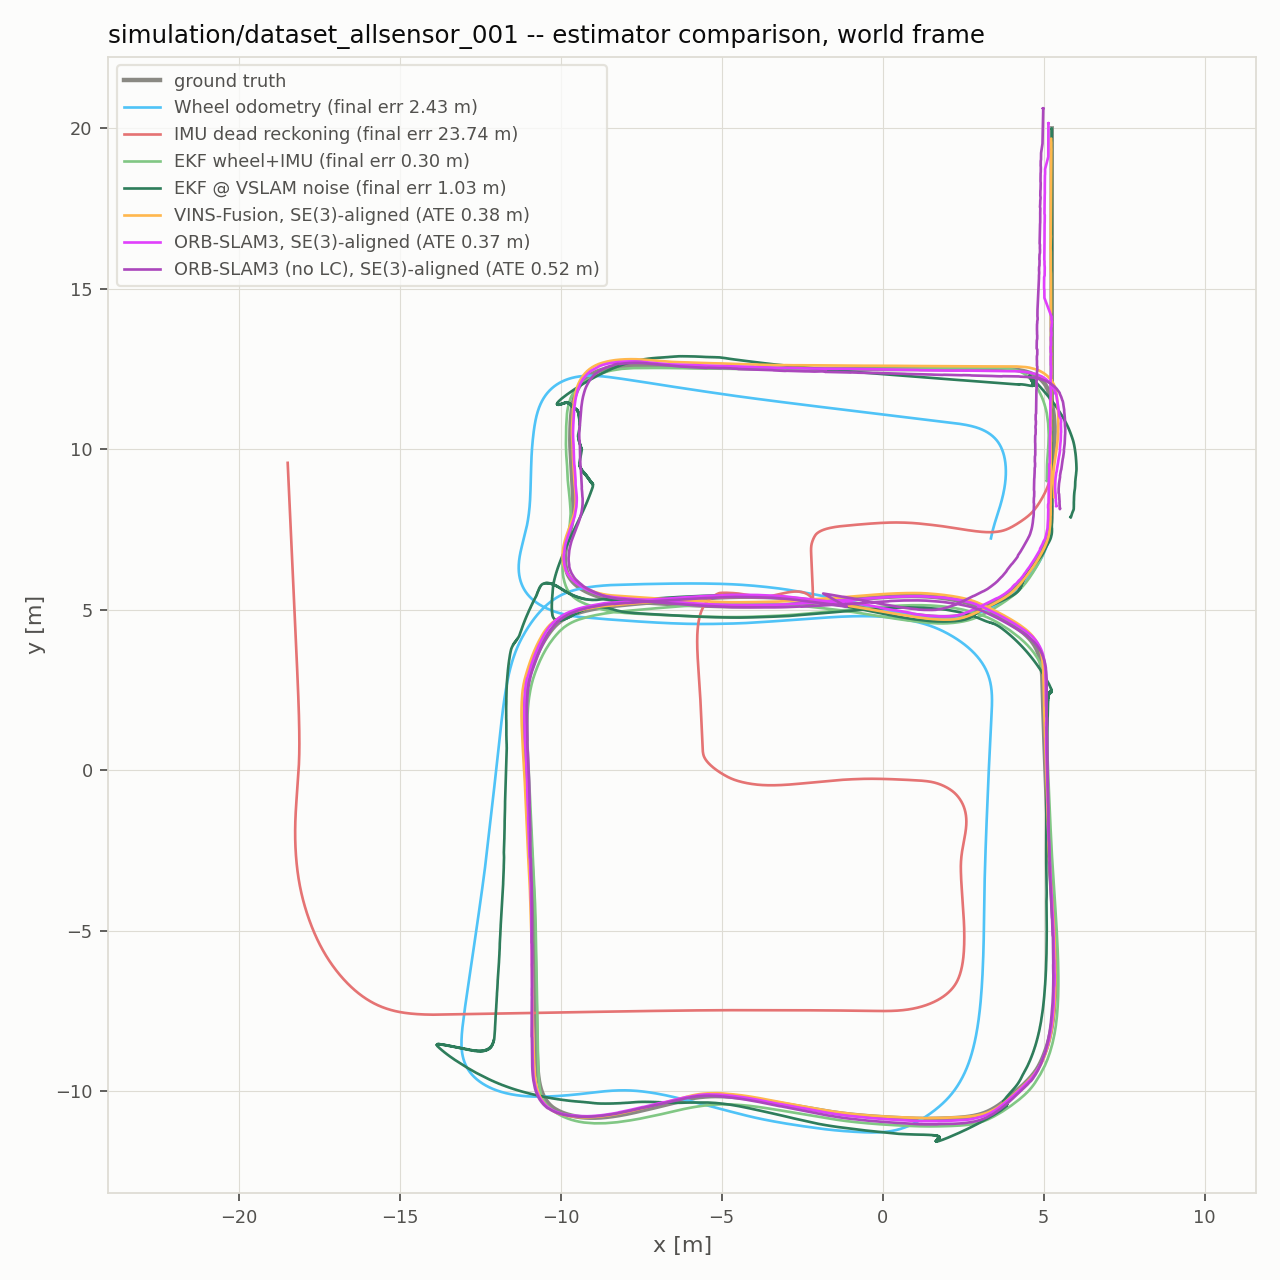
\includegraphics[width=0.82\textwidth]{../../../output/compare/simulation/exp-estimator-baseline/proprio_trajectories_dataset_allsensor_001_light.png}
  \caption[Estimator comparison on \repo{dataset_allsensor_001}, world frame.]{Estimator comparison on \repo{dataset_allsensor_001}, world frame. The
  baselines are drawn as estimated; the visual estimators are drawn after the same
  rigid $SE(3)$ alignment used for their metrics, because their own world frames
  are arbitrary. Ground truth is hidden beneath the EKF, VINS and ORB traces for
  most of the run. Wheel odometry (blue) bows consistently outward; IMU dead
  reckoning (red) leaves the building.}
  \label{fig:proprio-trajectories}
\end{figure}

\subsubsection{Falsification of H1, and the drift mechanism}
\label{sec:h1-falsified}

H1 is \flag{falsified} across all five datasets. If drift followed the fitted
yaw-rate scale, the bag with the most nearly correct scale would drift least. The
opposite holds (\cref{tab:h1}): \repo{allsensor_002} has the best scale of the
five, $+0.34\%$, and \SI{-30.11}{\degree} of heading error, while
\repo{allsensor_004} has the worst scale, $-7.50\%$, and only
\SI{-17.68}{\degree}. All five heading errors share a sign; the scale errors do
not.

\begin{table}[htbp]
\centering
\caption[Wheel-odometry heading drift against the fitted yaw-rate scale.]{Wheel-odometry heading drift against the fitted yaw-rate scale.
``Rotation'' is the total unsigned ground-truth rotation of the run, and
``error/rotation'' expresses the final heading error as a fraction of it. Scale
error and heading error correspond in neither sign nor magnitude. The last column
is the constant-offset prediction described below: the mean yaw-rate residual of
the run multiplied by its duration, which matches the measured error to within
\SI{1.4}{\degree} on every dataset, and to within \SI{0.5}{\degree} on three of
five.}
\label{tab:h1}
\small
\resizebox{\textwidth}{!}{%
\begin{tabular}{lrrrrr}
\toprule
Dataset & Yaw-rate scale & Final yaw error & Rotation & Error/rotation &
  Offset prediction \\
 & [\si{\percent}] & [\si{\degree}] & [\si{\degree}] & [\si{\percent}] &
  [\si{\degree}] \\
\midrule
\repo{allsensor_000} & $+1.10$ & $-13.76$ & 536 & $-2.566$ & $-13.81$ \\
\repo{allsensor_001} & $-4.73$ & $-12.95$ & 852 & $-1.519$ & $-13.37$ \\
\repo{allsensor_002} & $+0.34$ & \flag{$-30.11$} & 865 & $-3.481$ & $-31.03$ \\
\repo{allsensor_003} & $-6.25$ & \flag{$-37.17$} & 1123 & $-3.309$ & $-38.51$ \\
\repo{allsensor_004} & $-7.50$ & $-17.68$ & 895 & $-1.976$ & $-18.03$ \\
\bottomrule
\end{tabular}}
\end{table}

The proximate mechanism is nevertheless now identified, and it is simpler than a
scale error. The wheel model's yaw rate carries a small persistent \emph{offset}
against ground truth, averaged over all moving samples: \SI{-0.00277}{},
\SI{-0.00285}{} and \SI{-0.00624}{\radian\per\second} on the three bags. Because
heading is the time integral of that rate, an offset produces an error that grows
linearly with elapsed time rather than with rotation. Multiplying each offset by
its run duration reproduces the measured error to within \SI{1.4}{\degree} on all
five datasets (\cref{tab:h1}, last column), including the two textured-floor runs
that were recorded after the mechanism was proposed. The drift is accounted for.

\begin{queried}[Corrected]
An earlier reading of this experiment proposed that the offset came from the
bicycle model averaging the two kingpin angles, since $\tan$ of a mean is not the
mean of $\tan$. That explanation is \emph{wrong} and is withdrawn. Recomputing the
yaw rate as the mean of each wheel's own bicycle-equivalent rate changes the
residual from \SI{-0.00277}{} to \SI{-0.00288}{}, from \SI{-0.00285}{} to
\SI{-0.00296}{}, and from \SI{-0.00624}{} to \SI{-0.00630}{\radian\per\second}---
under \SI{4}{\percent} in every case, two orders of magnitude short of what the
observed drift requires. The averaging is not the source.
\end{queried}

What remains open is the origin of the offset itself. It is not a pure magnitude
error: splitting the residual by turn direction gives $+0.0109$ against $-0.0142$
on \repo{allsensor_000} and $+0.0075$ against
$-0.0292$~\si{\radian\per\second} on \repo{allsensor_002}, so the model
under-rotates in both directions \emph{and} carries a directional bias on top. On
\repo{allsensor_001}, whose route returns to its starting heading, both directions
are negative and only the bias is visible. A steering-angle zero offset, an
unmodelled slip angle, and a kingpin-geometry error are all consistent with what
has been measured so far and none has been tested.

This matters beyond wheel odometry, and the two textured-floor datasets turn what
was a caveat into a measurement. The EKF observes its gyroscope bias through
exactly this wheel yaw rate (\cref{sec:proprio-method}), so a persistent offset in
the wheel rate is absorbed into the estimated bias and reappears as heading error.
\Cref{tab:ekf-coupling} shows the two tracking each other across the five
datasets: where the wheel yaw-rate scale is within \SI{1.1}{\percent} of unity the
EKF holds heading to \SI{0.42}{\degree} or better, and where it is \SI{6}{} to
\SI{7.5}{\percent} low the EKF's heading error rises roughly tenfold.

\begin{table}[htbp]
\centering
\caption[The EKF's heading error follows the quality of the wheel yaw rate it uses to observe its gyroscope bias.]{The EKF's heading error follows the quality of the wheel yaw rate it uses
to observe its gyroscope bias. The filter is no better than its rate reference,
which is the cost of making the bias observable at all.}
\label{tab:ekf-coupling}
\small
\resizebox{\textwidth}{!}{%
\begin{tabular}{llrrrr}
\toprule
Dataset & Floor & Wheel yaw scale & Wheel yaw $\sigma$ & EKF yaw RMS & EKF ATE \\
 & & & [\si{\radian\per\second}] & [\si{\degree}] & [\si{\metre}] \\
\midrule
\repo{allsensor_000} & plain & 1.0110 & 0.0659 & 0.35 & 0.190 \\
\repo{allsensor_002} & plain & 1.0034 & 0.0705 & 0.30 & 0.256 \\
\repo{allsensor_001} & plain & 0.9527 & 0.0804 & 0.42 & 0.308 \\
\repo{allsensor_003} & bayline & 0.9375 & 0.1192 & \flag{3.54} & 0.423 \\
\repo{allsensor_004} & bayline & 0.9250 & 0.0613 & \flag{3.41} & 0.494 \\
\bottomrule
\end{tabular}}
\end{table}

An earlier version of this section, written when only the three plain-floor
datasets existed, recorded that the EKF held heading below \SI{0.7}{\degree}
everywhere and inferred that the absorbed error was small. \flag{That inference
does not survive the textured-floor datasets} and is withdrawn: the coupling is
the dominant term in the EKF's heading error whenever the wheel rate is poor, and
it sets a floor on the filter's accuracy that no amount of gyroscope quality can
lift.

One prediction of the original reasoning did survive, and is visible in
\cref{fig:proprio-covariance}: wheel-odometry error stays flat at roughly
\SI{6}{\milli\metre} for the first \SI{9.5}{\second}, the initial straight run,
and only grows once the first turn begins. Turning, not distance, starts the
error; the offset then sustains it.

\subsubsection{Covariance consistency}

H4 is supported emphatically. \Cref{tab:proprio-covariance} reports the average
normalised estimation error squared,
$\mathrm{NEES}=\mathbf{e}^{\top}\mathbf{P}^{-1}\mathbf{e}$ with
$\mathbf{e}=[\Delta x,\Delta y,\Delta\theta]$, which a correctly scaled covariance
makes average 3.0, together with the fraction of the run for which the truth lies
inside the reported $k\sigma$ bounds.

\begin{table}[htbp]
\centering
\caption[Covariance consistency of the non-visual estimators.]{Covariance consistency of the non-visual estimators. A consistent filter
gives $\mathrm{ANEES}=3.0$ and $\sigma$-coverages of 0.683, 0.954 and 0.997. Every
estimator is overconfident by roughly two orders of magnitude. Neither VINS-Fusion
nor ORB-SLAM3 writes a pose covariance, so neither can be tested here.}
\label{tab:proprio-covariance}
\small
\begin{tabular}{llrrrrl}
\toprule
Dataset & Estimator & ANEES & $1\sigma$ & $2\sigma$ & $3\sigma$ & Verdict \\
\midrule
\repo{allsensor_000} & Wheel odometry & 569.4 & 0.309 & 0.390 & 0.408 & overconfident \\
 & IMU dead reckoning & 311.0 & 0.005 & 0.022 & \flag{0.043} & overconfident \\
 & EKF wheel+IMU & 64.7 & 0.426 & 0.767 & 0.879 & overconfident \\
\midrule
\repo{allsensor_001} & Wheel odometry & 263.9 & 0.015 & 0.131 & 0.187 & overconfident \\
 & IMU dead reckoning & 339.9 & 0.001 & 0.009 & \flag{0.021} & overconfident \\
 & EKF wheel+IMU & 123.2 & 0.194 & 0.439 & 0.537 & overconfident \\
\midrule
\repo{allsensor_002} & Wheel odometry & 729.4 & 0.140 & 0.143 & 0.145 & overconfident \\
 & IMU dead reckoning & 244.7 & 0.017 & 0.045 & \flag{0.147} & overconfident \\
 & EKF wheel+IMU & 114.5 & 0.193 & 0.350 & 0.501 & overconfident \\
\midrule
\repo{allsensor_003} & Wheel odometry & 406.7 & 0.260 & 0.343 & 0.459 & overconfident \\
 & IMU dead reckoning & \flag{1504.3} & 0.010 & 0.018 & \flag{0.035} & overconfident \\
 & EKF wheel+IMU & 79.1 & 0.034 & 0.291 & 0.476 & overconfident \\
\midrule
\repo{allsensor_004} & Wheel odometry & 785.0 & 0.154 & 0.157 & 0.162 & overconfident \\
 & IMU dead reckoning & 289.5 & 0.004 & 0.017 & \flag{0.044} & overconfident \\
 & EKF wheel+IMU & 78.6 & 0.254 & 0.330 & 0.570 & overconfident \\
\midrule
\multicolumn{2}{l}{\emph{consistent reference}} & 3.0 & 0.683 & 0.954 & 0.997 & -- \\
\bottomrule
\end{tabular}
\end{table}

The IMU case is the starkest: its $3\sigma$ envelope contains the truth for
between \SI{2.1}{\percent} and \SI{14.7}{\percent} of each run, and its worst
ANEES, 1504 on \repo{allsensor_003}, is the largest figure in the experiment.
A consumer weighting this estimate by its stated covariance---a costmap, a
pose-graph edge, a relocaliser gate---would trust it tens of times more than it
deserves. Wheel odometry on \repo{allsensor_002} is the single worst case in the
experiment, ANEES 785 on \repo{allsensor_004} with $3\sigma$ coverage of 0.162, which is
consistent with
the heading offset of \cref{sec:h1-falsified}: the covariance model contains no
term for a persistent rate bias, so the larger that bias, the further the claimed
uncertainty falls behind the real error. The EKF is the least bad on every
dataset, at $3\sigma$ coverage between 0.476 and 0.879, and
\cref{fig:proprio-covariance} shows why: its NEES is genuinely near 3 during the
opening straight and only departs once turning begins, which is the same moment
the unmodelled heading error appears.

\begin{figure}[htbp]
  \centering
  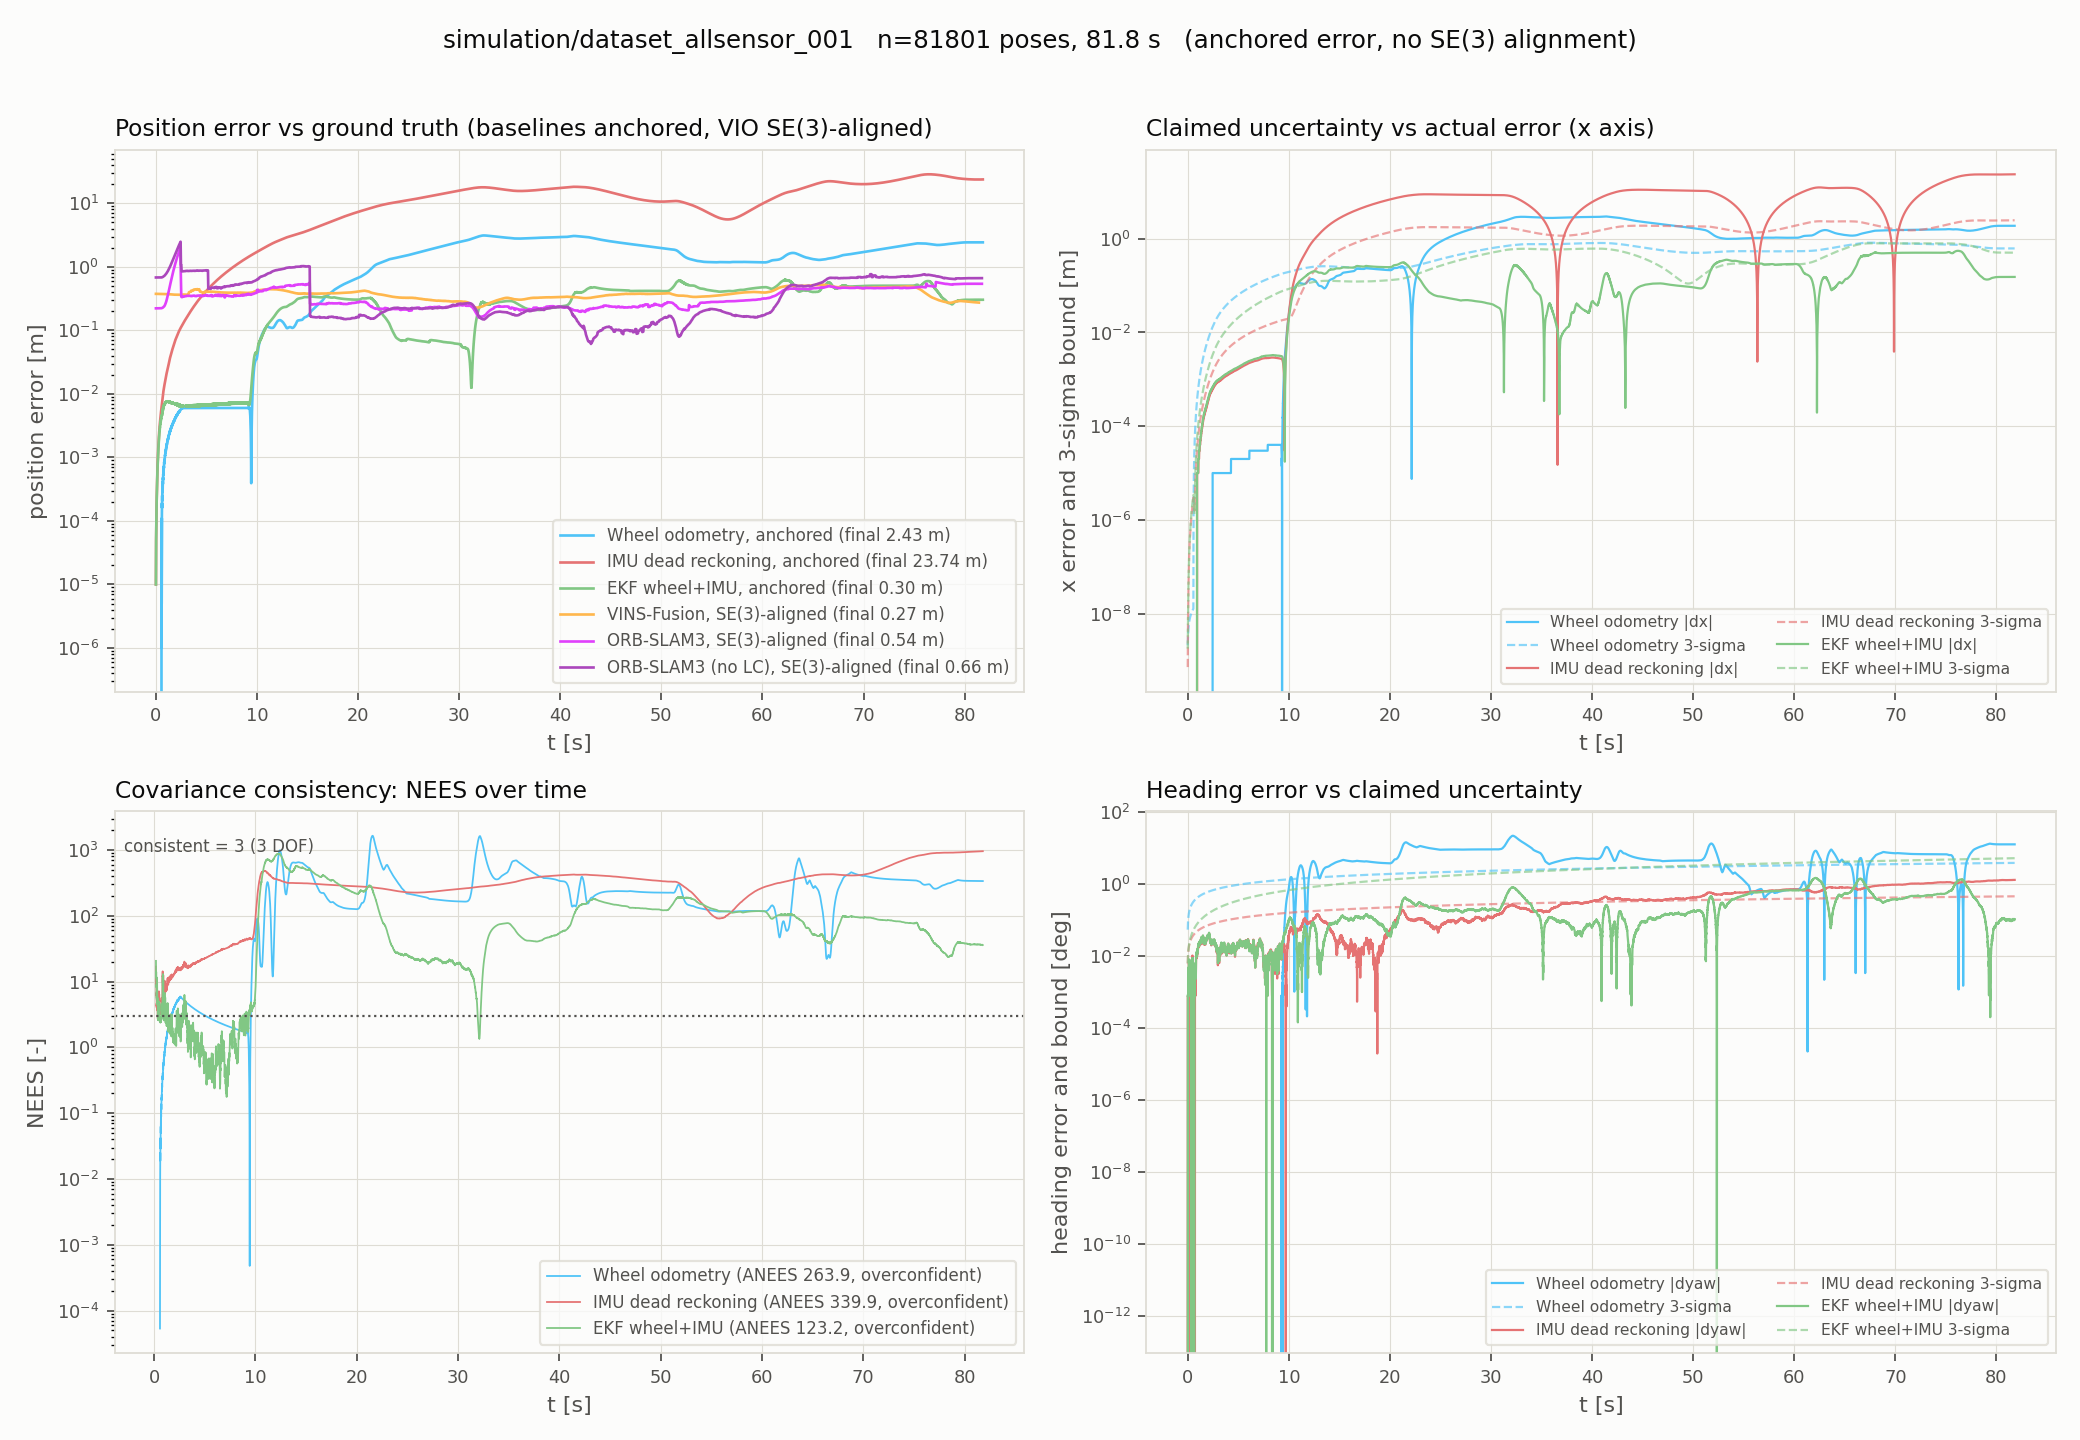
\includegraphics[width=\textwidth]{../../../output/compare/simulation/exp-estimator-baseline/proprio_covariance_dataset_allsensor_001_light.png}
  \caption[Error against claimed uncertainty for \repo{dataset_allsensor_001}.]{Error against claimed uncertainty for \repo{dataset_allsensor_001}.
  Top left: position error over time, baselines anchored and visual estimators
  $SE(3)$-aligned. Top right and bottom right: absolute error against the
  estimator's own $3\sigma$ bound, in $x$ and in heading; where the solid line
  sits above the dashed line of the same colour the filter is overconfident.
  Bottom left: NEES against the consistent value of 3. The step near
  \SI{9.5}{\second} in every panel is the first turn of the run.}
  \label{fig:proprio-covariance}
\end{figure}

\begin{queried}[Method caveat]
The $\chi^2$ interval behind the verdict column assumes independent samples. At
\SI{200}{\hertz} consecutive dead-reckoning errors are almost perfectly
correlated, so the test is run on a \SI{1}{\hertz} subsample (81 to 102 samples per dataset).
That reduces the dependence but does not remove it, and the verdicts should be
read as indicative. The $\sigma$-coverage columns make no independence assumption
and are the sturdier statement.
\end{queried}

\subsubsection{Cross-validation of the EKF noise model}

The EKF's noise model is derived from the same recording it runs on, whereas the
visual estimators receive no comparable tuning. The wheel and IMU baselines are
unaffected---their measured $\sigma$ values enter only the covariance, never the
trajectory---but the EKF's values enter the Kalman gain and so do change its
output. The comparison was therefore repeated with the noise models exchanged
between bags (\cref{tab:proprio-xval}).

\begin{table}[htbp]
\centering
\caption[EKF accuracy with an in-sample and an out-of-sample noise model.]{EKF accuracy with an in-sample and an out-of-sample noise model. The
change is negative on four of five bags---the borrowed model is \emph{better}
there---and the mean change is about $-10\%$, which is the signature of no
systematic in-sample advantage.}
\label{tab:proprio-xval}
\small
\begin{tabular}{llrr}
\toprule
Dataset & Noise model from & Aligned ATE [\si{\metre}] & Change \\
\midrule
\repo{allsensor_000} & same bag & 0.190 & -- \\
 & \repo{allsensor_001} & 0.206 & $+8.8\%$ \\
\midrule
\repo{allsensor_001} & same bag & 0.308 & -- \\
 & \repo{allsensor_000} & 0.263 & $-14.5\%$ \\
\midrule
\repo{allsensor_002} & same bag & 0.256 & -- \\
 & \repo{allsensor_000} & 0.220 & $-13.9\%$ \\
\midrule
\repo{allsensor_003} & same bag & 0.423 & -- \\
 & \repo{allsensor_000} & 0.392 & $-7.1\%$ \\
\midrule
\repo{allsensor_004} & same bag & 0.494 & -- \\
 & \repo{allsensor_000} & 0.377 & $-23.8\%$ \\
\bottomrule
\end{tabular}
\end{table}

The noise model transfers between runs, and on four of the five bags the borrowed
model is the better one, which no in-sample advantage could produce. The EKF's
accuracy is therefore a property of the estimator rather than of having seen the
answer. Cross-validated it reaches 0.206, 0.263, 0.220, 0.392 and
\SI{0.377}{\metre}, which is 1.38, 1.41, 2.53, 1.31 and 1.13 times better than the
best visual estimator of each dataset. Notably the cross-validated figure on
\repo{allsensor_004} recovers a lead that the in-sample filter did not have.

\begin{queried}[What this control does not cover]
Exchanging noise models between bags tests whether the filter saw \emph{this}
recording's answer. It cannot test the asymmetry that matters here, because both
models are still measured from data: all five bags come from one simulated IMU, so
the exchanged $\sigma$ values differ by less than a factor of two on every term
except accelerometer $x$. The visual estimators receive nothing of the kind---they
read four constants from a file. The control in \cref{sec:proprio-tuning} replaces
this one.
\end{queried}

\subsubsection{Transferring the visual systems' noise model to the EKF}
\label{sec:proprio-tuning}

\paragraph{Question and hypothesis.}
Is the EKF's advantage in \cref{tab:proprio-accuracy} an estimator effect or a
noise-model effect? Stated as a falsifiable hypothesis, \textbf{H4}: the EKF's
advantage survives being given the visual systems' own IMU noise configuration.
H4 is falsified if, on that configuration, the EKF's mean aligned ATE over the
five bags is no better than VINS-Fusion's.

\paragraph{Conditions and controls.}
The asymmetry is measured against declared, not bag against bag. VINS-Fusion and
ORB-SLAM3 both read \repo{config/wil_sim/stereo_imu.yaml}, and every one of the
fifteen visual runs in \cref{tab:proprio-accuracy} records that file in its
metadata---the five VINS runs \repo{logging_20260916_01}, and the ten ORB runs
\repo{_01} and \repo{_02}---so a single hand-set configuration stands behind the
whole visual column. The cheap half of the control is therefore to re-run the
filter on that same file. It needs no new recording: the EKF reads the bags
offline.

The independent variable is the four IMU noise terms, at three levels: the
measured per-bag values, the values \repo{stereo_imu.yaml} declares, and a set of
one-term-at-a-time ablations between them. Held fixed across every condition are
the five bags, the ground truth and its interval, the filter code and commit, the
bicycle yaw-rate model, the \SI{50}{\hertz} wheel-update stride, and the
alignment convention. The accelerometer and gyroscope biases and the whole wheel
block stay at their measured values, so the IMU noise model is the only treatment;
the single exception is the $R$-only ablation described below, which moves the
wheel yaw-rate $\sigma$ by construction. Converting the file's densities to the
per-sample $\sigma$ the filter stores ($\sigma = n\sqrt{f}$,
$f = \SI{200}{\hertz}$) gives a gyroscope term 5.5 to 6.7 times the measured
value, an accelerometer term between 0.68 and 1.44 times it, and a bias random
walk ten times it.

\paragraph{Validity and sample count.}
$n=1$ run per bag per condition, thirty runs in all. The filter is deterministic
given a bag and a noise model, so repeats would be bit-identical and no
run-to-run uncertainty can be quoted; the spread reported below is across
\emph{bags}, not runs, and is given as a range rather than a standard deviation.
All thirty completed, produced the same pose counts as their measured-noise
counterparts (17\,416, 16\,364, 17\,350, 20\,477 and 20\,104), applied the same
number of wheel corrections, and were scored over the same matched interval
against the same ground truth. The measured-noise condition is the published
baseline and was not re-run. Re-scoring it through this experiment's own code
reproduces \cref{tab:proprio-accuracy} to three decimals, which is the check that
the two paths agree.

\paragraph{Results.}
Those are the \emph{EKF @ VSLAM noise} rows of \cref{tab:proprio-accuracy}.

The result reverses the section. Mean aligned ATE over the five bags rises from
\SI{0.334}{\metre} to \SI{1.135}{\metre}, a degradation on every bag without
exception. Against that figure VINS-Fusion's \SI{0.553}{\metre} wins on
\emph{five of five}, ORB-SLAM3 without loop closing (\SI{0.804}{\metre}) on four
of five, and ORB-SLAM3 with loop closing on four of five---its mean of
\SI{1.854}{\metre} is set by the \repo{allsensor_003} outlier, and its median of
\SI{0.602}{\metre} is the fairer summary. On the metric this chapter uses
throughout, run on the tuning the visual systems actually had, both visual systems
are ahead of the filter.

\Cref{tab:proprio-tuning-ablation} locates the cause. Moving the four terms one at
a time shows that the gyroscope noise density accounts for essentially all of the
damage; the accelerometer term is inert and the bias random walk contributes
little. The density enters the filter twice---as heading process noise in $Q$, and
in the bias observation's $R$ as $\sigma_{w}^{2} + \sigma_{g}^{2}$. Raising the
wheel yaw-rate $\sigma$ so that $R$ matches the transferred case exactly while $Q$
stays measured reproduces the baseline, so the damage is entirely in $Q$. A
gyroscope density $6.5\times$ too loose inflates the heading process variance
forty-fold, and because the measurement matrix touches only $v$ and $b_{\omega}$,
heading can then be corrected only through the $P_{2,3}$ and $P_{2,4}$ cross
terms---so the wheel yaw-rate residual begins steering heading instead of staying
confined to the bias. Anchored yaw RMS rises from \SI{1.60}{\degree} to
\SI{8.67}{\degree}.

Relative pose error confirms the attribution independently, and on a local metric
that no global alignment can flatter. At $\Delta=\SI{1}{\second}$ the transferred
model degrades translation from \SIrange{0.100}{0.493}{\metre} and rotation from
\SIrange{0.285}{2.262}{\degree}; the gyroscope-only ablation reaches
\SI{0.485}{\metre} and \SI{2.179}{\degree}, almost all of it, while the
accelerometer ablation is indistinguishable from the measured model to three
decimals. The $R$-only case is marginally \emph{better} than the measured model
on all three metrics and on every bag, which says the measured wheel yaw-rate
$\sigma$ is itself slightly too tight and confirms that the $R$ path is benign
rather than merely null.

\begin{table}[htbp]
\centering
\caption[Which of the four IMU noise terms costs the EKF its accuracy.]{Which of the four IMU noise terms costs the EKF its accuracy. Each row
moves one term from its measured value to the one
\repo{config/wil_sim/stereo_imu.yaml} declares, averaged over the five bags. The
last row isolates where the gyroscope term acts: it reproduces that term's effect
on the measurement noise $R$ exactly, by raising the wheel yaw-rate $\sigma$,
while leaving the process noise $Q$ at its measured value.}
\label{tab:proprio-tuning-ablation}
\small
\begin{tabular}{lrrr}
\toprule
EKF, one term moved & Anchored RMS & Aligned ATE & Anchored yaw RMS \\
 & [\si{\metre}] & [\si{\metre}] & [\si{\degree}] \\
\midrule
measured throughout & 0.484 & 0.334 & 1.60 \\
gyroscope density, $\times 6.5$ & 1.654 & 1.105 & 8.67 \\
accelerometer density & 0.479 & 0.329 & 1.60 \\
gyroscope bias random walk, $\times 10$ & 0.654 & 0.452 & 2.97 \\
all four (\emph{EKF @ VSLAM noise}) & 1.693 & 1.135 & 8.88 \\
\midrule
gyroscope density through $R$ only & 0.475 & 0.327 & 1.50 \\
\bottomrule
\end{tabular}
\end{table}

\paragraph{Interpretation.}
Two findings survive the control and one does not. ORB-SLAM3's rotational error
stays at 13.6 to \SI{16.5}{\degree} in every condition, still
\num{2.4} times worse than the handicapped filter's \SI{6.21}{\degree}, so that
result is a property of ORB-SLAM3 and not of tuning. The complementary-failure
mechanism of the two proprioceptive sensors is likewise untouched, since it does
not depend on which $\sigma$ the filter was given. What does not survive is the
ranking of the EKF against the visual estimators.

The consistency picture moves the other way, and is worth stating because it is
the one place the transferred model does better. The EKF's ANEES falls from 64.7
to 123.2 down to 12.6 to 38.3---still overconfident by more than an order of
magnitude, but far less so. A loose noise model buys a covariance closer to
honest at the cost of the estimate itself, which is the textbook trade and is the
first time this chapter has been able to show it directly.

\paragraph{Limitations.}
\begin{queried}[What the control does and does not establish]
\flag{H4 was written down after the exploratory runs had been scored, not
before.} What is reported here is a post-hoc formalisation of an exploratory
finding; the decision rule and the direction of the test were fixed before this
subsection was written, but not before the data was seen. The unanimity---every
bag, both directions, a mechanism that isolates to one term---is what makes it
worth reporting at this stage, not a pre-registered test, and a confirmatory
repeat on bags not used to form the hypothesis is the honest follow-up.

This is also an equal-handicap comparison, not an equal-effort one: both families
now run on a declared IMU noise that nobody fitted to the data. It establishes
that the EKF's advantage in \cref{tab:proprio-accuracy} is smaller than the
tuning difference between the two families, and reverses under it. It does
\emph{not} establish that the visual systems would win a symmetric comparison.
The mirror experiment---giving VINS-Fusion and ORB-SLAM3 the measured
values---requires re-recording and has not been run to a reportable standard; the
one VINS run whose metadata confirms it diverged (\cref{sec:sim-fidelity}). The
transfer is not perfectly symmetric in role either: the filter's $\sigma_{g}$ is
a scalar in a planar five-state model, whereas \repo{gyr_n} feeds three-axis
pre-integration. Finally, $n=1$ per cell is a property of a deterministic filter
and not a design choice, but it means the between-bag range is the only
uncertainty this experiment can report.
\end{queried}

\subsubsection{Interpretation and limitations}

Across these five recordings, a five-state planar filter over wheel encoders and a
gyroscope localises more accurately than either stereo visual-inertial system
\emph{when its noise model is calibrated per bag and theirs is not}. Under the
tuning control of \cref{sec:proprio-tuning} that ordering reverses on every bag,
so the uncomfortable result for the thesis premise is weaker than it first
appeared: what these bags demonstrate is that the noise model is worth more than
the architecture over this range, not that dead reckoning outperforms vision. The
practical reading is unchanged in one respect and sharpened in another. It still
does not show that vision is unnecessary, and the justification for it still has
to come from capabilities dead reckoning does not have at all---loop closure,
relocalization after tracking loss, and the map itself---or from conditions these
bags do not contain. It now also shows that the visual systems have never been
tuned to this platform, which is the cheapest remaining source of improvement and
is the first item of \cref{sec:results-discussion}.

\begin{queried}[Generalisation limit]
The comparison is confined to \emph{static} scenes. Four worlds and both floor
conditions are now covered and the ranking is stable across them, so the earlier
form of this limitation---that the result held only on featureless floors, vision's
worst case---is no longer the binding one. \flag{Adding the bay markings did not improve
either visual estimator}, which removes that explanation rather than confirming
it---though the markings are a much weaker manipulation than ``textured floor''
suggests (\cref{fig:floor-treatments}), so a genuinely textured surface remains
untested.

What remains is that every dataset carrying wheel encoders is static
(\cref{tab:dataset-registry}). The result must not be restated as
``proprioception outperforms visual SLAM'' without that qualifier, and it cannot
be extended to dynamic scenes---where wheel odometry is unaffected by moving
objects, and where the visual systems' known failures occur---until the
\repo{allsensor} topics are recorded in a dynamic world. That recording remains
the single most informative next run in this line of work.
\end{queried}

\begin{queried}[Queried]
Both visual estimators replayed their bags at $0.5\times$ real time, so each frame
received roughly twice the wall-clock budget it would have online. The accuracy
figures in \cref{tab:proprio-accuracy} are therefore not evidence of real-time
capability, and no timing conclusion may be drawn from this experiment. The three
baselines, being offline, have no replay rate at all, which is a second asymmetry
in the same comparison.
\end{queried}

\begin{queried}[Statistical limit]
$n=5$ across four worlds, and no condition is repeated more than twice. The tables
therefore report individual values deliberately; no mean, standard deviation or
confidence interval is computed, and between-dataset differences are not evidence
of a systematic effect. A single run per world cannot establish a scene-content
effect; it shows only that the estimator ranking survives changes of scene.
\end{queried}

\begin{queried}[Unmeasured variance]
ORB-SLAM3 is multi-threaded and not deterministic, and its run-to-run spread on
identical input has not been measured here: each of its two configurations was run
once per dataset. Several differences this chapter reports sit within a range that
spread could plausibly cover---most sharply \SI{6.481}{\metre} with loop closing
enabled on \repo{allsensor_003} against \SI{0.515}{\metre} with it disabled, and
the reversal on \repo{allsensor_002} where disabling it is three times
\emph{worse}. Those differences are real measurements of the runs that were made,
but they cannot yet be attributed to the loop-closing switch. Three or more
repeats per configuration, reported as median and spread in the manner of the
relogged campaign (\cref{sec:results-validity}), are required before any
loop-closure conclusion is drawn.
\end{queried}

Two further limitations are structural rather than queried. All three baselines
begin from the ground-truth pose, because dead reckoning has no global reference;
a deployed system would have to obtain that pose some other way, which is exactly
the relocalization problem listed as future work. And the covariance result cannot
yet be extended to the visual estimators, because neither writes a pose
covariance---adding that to VINS-Fusion's marginalisation output is an
instrumentation change, not an analysis one, and is the prerequisite for applying
this consistency test to the pipelines the thesis is actually about.


\paragraph{Summary.} IMU-only dead reckoning drifts by \SIrange{12.6}{45.6}{\metre}
and wheel odometry by \SIrange{1.0}{3.2}{\metre} of aligned ATE; the EKF stays
below \SI{0.5}{\metre} on every recording and the visual estimators between
\SI{0.29}{} and \SI{0.78}{\metre} in their best configuration. The EKF's lead
over vision is a tuning effect, not an architectural one: with the visual
systems' own inertial noise model it loses to VINS-Fusion on all five bags. The
two proprioceptive sensors fail in complementary ways, and every dead-reckoning
covariance is overconfident by roughly two orders of magnitude. Against the
project's target of \SI{0.05}{\metre} ATE, no estimator in this slot qualifies.

\paragraph{Future plan.} Feed the VIO pose into the EKF as a third measurement,
so that the filter takes distance from the wheels, heading from the gyroscope
and drift correction from vision; and re-run in a realistic environment with
wheel slip and encoder quantisation, since both idealisations of
\cref{sec:sim-fidelity} favour dead reckoning.

\subsection{Real robot}
\label{sec:exp1-real}

\slotstatus{planned}{No real recording carries wheel odometry or joint states,
and none carries an independent ground truth, so neither the baselines nor
their scoring can be computed.}

\textbf{Reason.} Of the three real recordings (\cref{tab:dataset-registry}) only
\repo{dataset_real_000} has inertial data, and none has the
\repo{/model/.../joint_state} and \repo{odometry} topics the wheel and EKF
estimators consume. The motion-capture reference of \cref{sec:real-site} has
not yet been recorded with the robot.

\textbf{Next action.} Bridge the wheel encoder and steering topics on the real
platform, record the motion-capture trajectory alongside the sensors, and
repeat the process of \cref{sec:results-proprio} unchanged; the calibration
pass will then also give the first measured noise model of the real IMU.

% =====================================================================
\section{Experiment 2: Offline YOLO Detector Performance}
\label{sec:exp2}

\subsection{Simulation}
\label{sec:yolo-performance}

\slotstatus{completed}{Four dynamic recordings, 9\,860 left-camera frames,
scored against projected simulator ground truth at the thresholds of
\cref{tab:yolo-eval-params}.}

\textbf{Objective.} Measure detector localization and class assignment
independently of either SLAM integration (\cref{sec:yolo-eval-method}).

\textbf{Process.} \repo{script/yolo_eval.py} projected the collision meshes of
every prop into \repo{cam0} to form truth boxes, ran the project checkpoint
\repo{weight/best.pt}, matched predictions greedily by class at IoU 0.5, and
wrote per-frame and per-detection records; overlays were inspected before the
aggregates were accepted.

\textbf{Dataset.} The four \repo{dataset_dynamic_nofloortexture} recordings of
\cref{tab:dataset-registry}.

% Verbatim from minor_report/chapters/chapter_4_results.tex lines 917-1038 (retired report),
% headings demoted by 1 level(s). Do not edit here; edit the source of the numbers.

YOLO was evaluated independently of either SLAM integration on all four dynamic
no-floor-texture rosbags. Ground-truth object poses came from
\repo{/world/default/pose/info}; because that topic's message headers are zero,
its rosbag receive times were mapped to simulation time by interpolation against
the recorded \repo{/clock} stream. Known model meshes were transformed into the
camera frame and projected into \repo{cam0} to form two-dimensional boxes.
Sampled overlays from every bag were inspected before calculating metrics and
showed spatially plausible agreement between the projected boxes and visible
objects.

\subsubsection{Bounding-Box Detection and Localization}
\label{sec:yolo-bbox}

The evaluation used 9,860 camera frames, confidence threshold 0.35, NMS IoU
threshold 0.50, and matching IoU threshold 0.50. Ground-truth
boxes smaller than 12 pixels on either side were omitted; heavily occluded
ground-truth boxes and predictions explained by explicitly unlabelled scenery
were ignored rather than counted as errors. Table~\ref{tab:yolo-performance}
reports per-dataset results and a micro-average formed by pooling TP, FP, and FN
counts across all frames.

\begin{table}[htbp]
\centering
\caption[Offline YOLO performance against projected Gazebo object ground truth.]{Offline YOLO performance against projected Gazebo object ground truth.
This is a detector-capability measurement, not an evaluation of delivery to the
online SLAM filters.}
\label{tab:yolo-performance}
\resizebox{\textwidth}{!}{%
\begin{tabular}{lrrrrrrrr}
\toprule
Dataset & Frames & TP & FP & FN & Precision & Recall & F1 & Moving recall \\
\midrule
Dynamic 00/000 & 2,347 & 9,987 & 4,826 & 5,900 & 0.674 & 0.629 & 0.651 & 0.617 \\
Dynamic 00/001 & 2,236 & 10,158 & 4,265 & 6,868 & 0.704 & 0.597 & 0.646 & 0.599 \\
Dynamic 01/000 & 2,564 & 8,142 & 4,226 & 6,064 & 0.658 & 0.573 & 0.613 & 0.568 \\
Dynamic 02/000 & 2,713 & 8,661 & 3,743 & 6,502 & 0.698 & 0.571 & 0.628 & 0.581 \\
\midrule
Pooled & 9,860 & 36,948 & 17,060 & 25,334 & 0.684 & 0.593 & 0.635 & 0.591 \\
\bottomrule
\end{tabular}}
\end{table}

The pooled evaluation contains 62,282 scored ground-truth boxes, of which 46,491
are moving, plus 34,476 projected boxes excluded as heavily occluded. The model
produced 58,776 raw predictions. Mean image coverage was 10.42\% for all scored
ground truth, 7.88\% for moving ground truth, and 9.07\% for predictions. At the
stated thresholds, the detector misses approximately 41\% of scored moving
objects; moving-object recall ranges from 0.568 to 0.617 between datasets.
Conversely, the results demonstrate that the trained model can produce detections
on every recorded bag. They do not contradict the zero-box VINS+YOLO logging
anomaly: offline detector capability and online message delivery/timestamp
matching are different mechanisms. Average precision is not reported because
this evaluation retained predictions only above a single confidence threshold.

\begin{figure}[htbp]
  \centering
  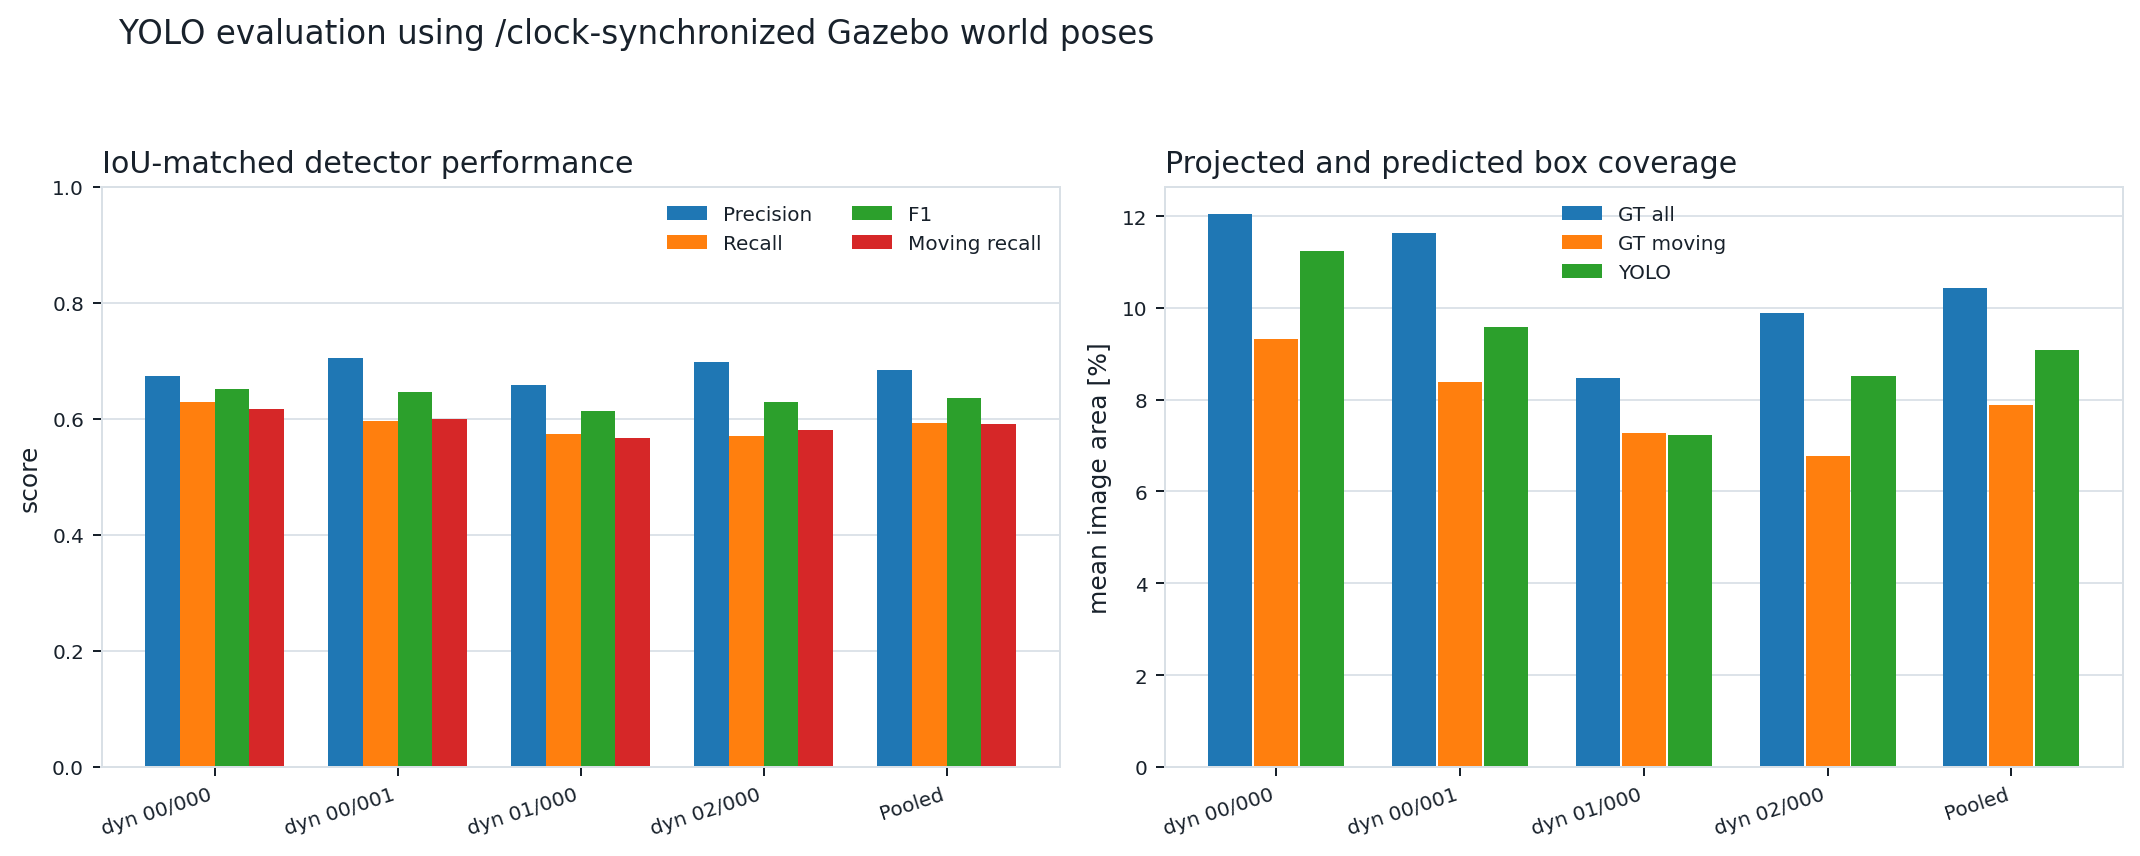
\includegraphics[width=\textwidth]{../../../output/yolo_eval/summary_light.png}
  \caption[Per-dataset and pooled detector scores and box-area coverage.]{Per-dataset and pooled detector scores and box-area coverage. Pooled
  precision, recall, F1, and moving-object recall are calculated from pooled
  counts, rather than by averaging the four displayed dataset scores.}
  \label{fig:yolo-performance-summary}
\end{figure}

\begin{figure}[htbp]
  \centering
  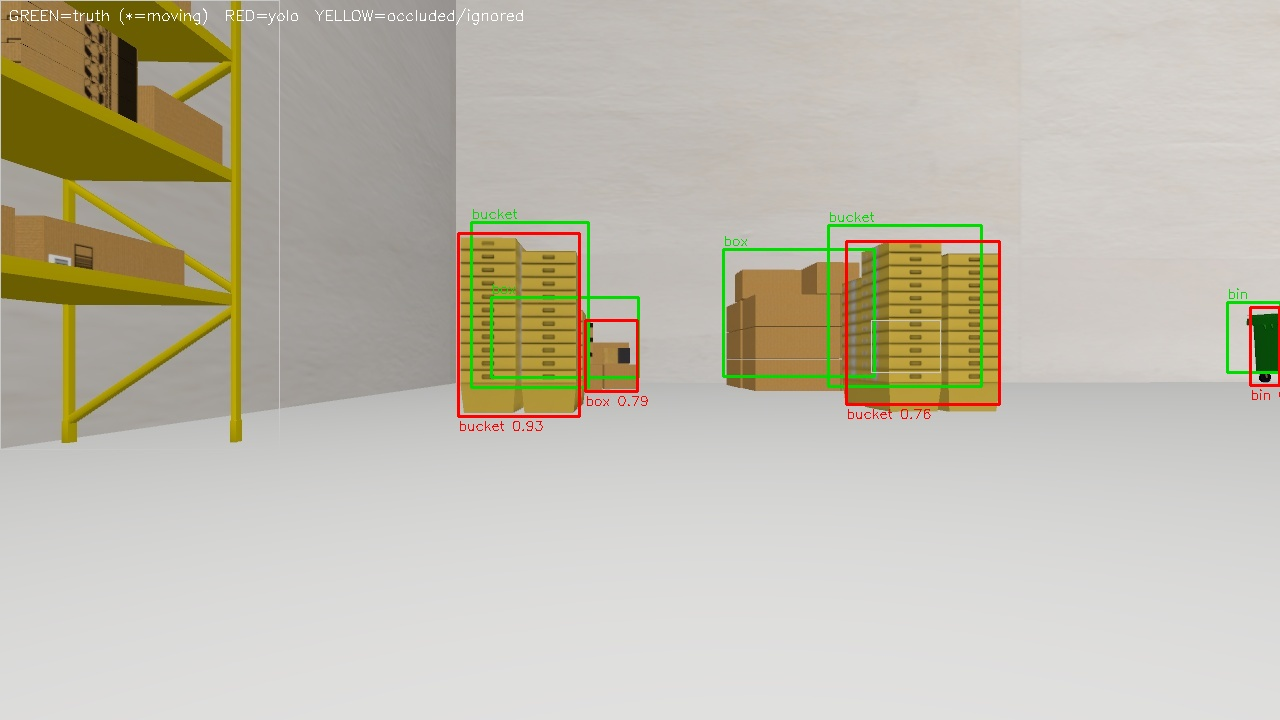
\includegraphics[width=\textwidth]{../../../output/yolo_eval/dyn_00_001/overlay/01116.jpg}
  \caption[Representative validation overlay used before accepting the offline metrics.]{Representative validation overlay used before accepting the offline
  metrics. Green boxes are projected ground truth and red boxes are YOLO
  predictions. A \textbf{yellow} box is a ground-truth object that a nearer
  object covers by more than \SI{70}{\percent}; it is excluded from scoring, so
  the detector is neither credited for finding it nor penalised for missing it.
  Only the green boxes are scored. An asterisk marks a ground-truth object
  classified as moving from its world-pose history.}
  \label{fig:yolo-ground-truth-overlay}
\end{figure}

\clearpage
\subsubsection{Object-Class Assignment Conditional on Localization}
\label{sec:yolo-classification}

This experiment is not whole-image classification: an image can contain many
objects, and the model outputs a class for each predicted bounding box. To keep
class assignment separate from localization, predictions and ground-truth boxes
were greedily associated by IoU $\geq0.50$ without requiring their classes to
agree. Classification was then evaluated only on the 37,061 localized object
pairs. Missed ground-truth objects and unmatched predictions remain bounding-box
detection errors in Section~\ref{sec:yolo-bbox}; they are not treated as an
additional semantic class here.

\begin{table}[htbp]
\centering
\caption{Object-class assignment conditional on successful IoU association,
pooled across the four dynamic datasets.}
\label{tab:yolo-classification}
\begin{tabular}{lrrrr}
\toprule
Class & Associated objects & Precision & Recall & F1 \\
\midrule
Bin & 2,639 & 1.000 & 1.000 & 1.000 \\
Box & 28,076 & 0.996 & 0.999 & 0.998 \\
Bucket & 6,346 & 0.996 & 0.983 & 0.989 \\
\midrule
Macro average & 37,061 & 0.997 & 0.994 & 0.995 \\
\bottomrule
\end{tabular}
\end{table}

The conditional class accuracy is 0.996: 36,924 of 37,061 associated objects
are on the confusion-matrix diagonal, leaving 137 class substitutions. The
largest substitution is 110 buckets labelled as boxes. This high conditional
accuracy does not cancel the weaker bounding-box recall: an object that was
never localized cannot enter the conditional class-assignment evaluation.

\begin{figure}[htbp]
  \centering
  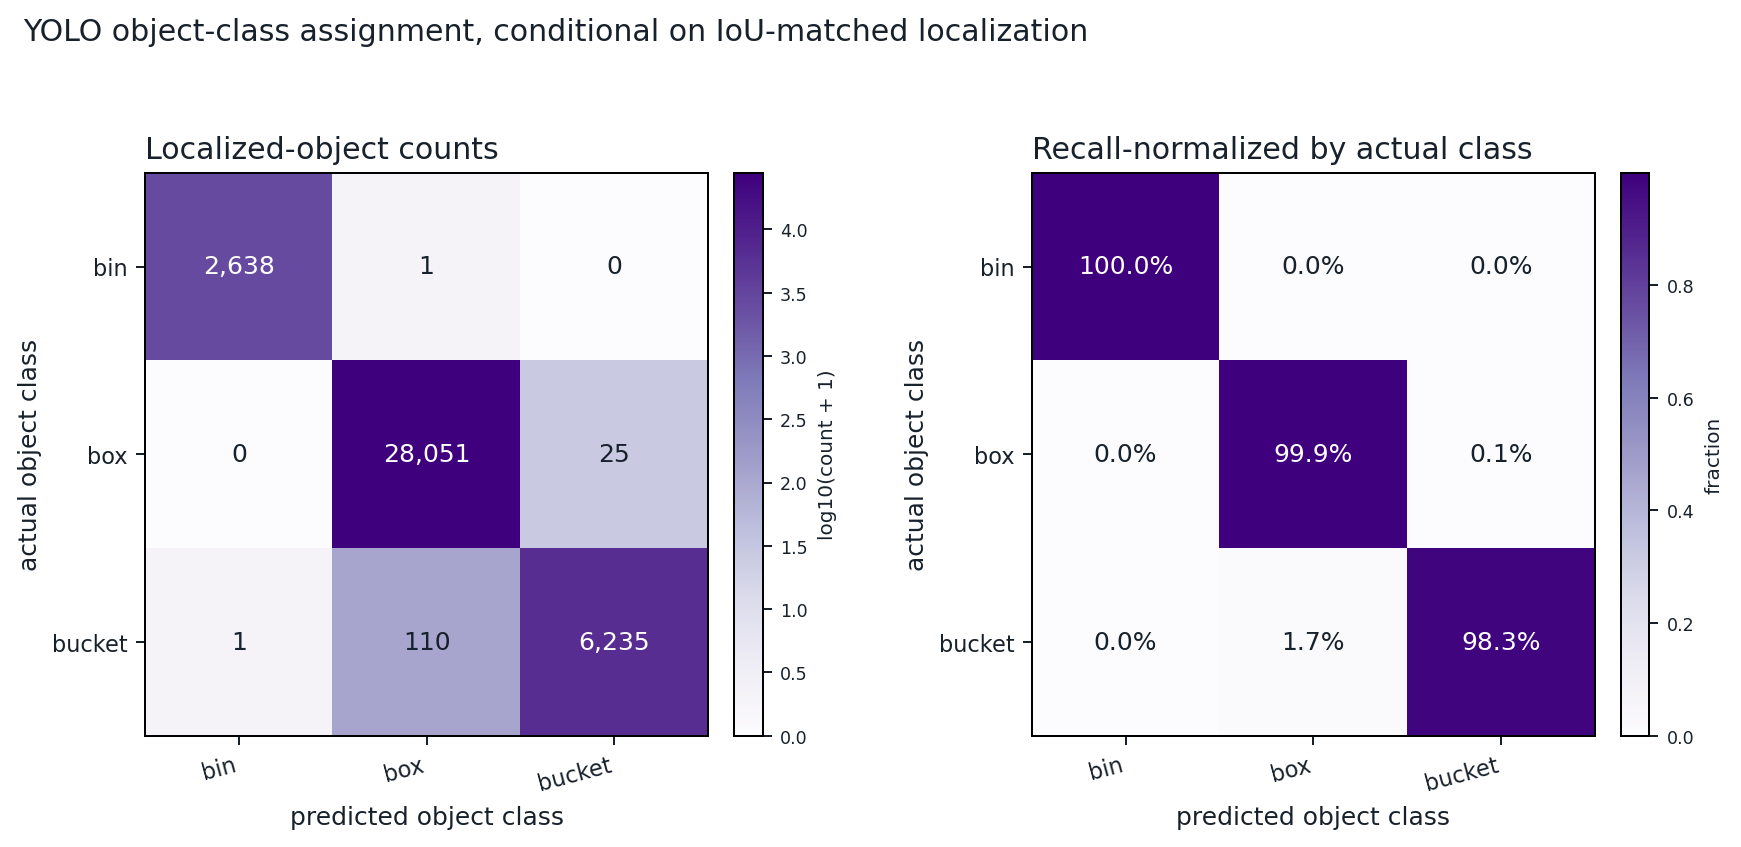
\includegraphics[width=\textwidth]{../../../output/yolo_eval/classification_confusion_light.png}
  \caption[Object-class confusion conditional on class-agnostic IoU association.]{Object-class confusion conditional on class-agnostic IoU association.
  Rows are actual object classes and columns are predicted object classes. The
  left panel gives counts on a logarithmic colour scale; the right panel
  normalizes within each actual class. Background is intentionally excluded.}
  \label{fig:yolo-classification-confusion}
\end{figure}


\paragraph{Summary.} The detector is reliable at naming and unreliable at
finding: pooled precision 0.684, moving-object recall 0.591, conditional class
F1 0.995. The \SI{41}{\percent} of moving objects it misses is the limit any
downstream filter inherits, and it is computed over the easier, exemption-filtered
subset; counting every exempt object as a miss gives a recall of 0.382.

\paragraph{Future plan.} Validate the projected ground truth against manual
annotation on a frame subset; add object velocity from consecutive detections
so that the mask targets moving objects rather than object classes; and re-run
on the realistic warehouse environment once it is built.

\subsection{Real robot}
\label{sec:exp2-real}

\slotstatus{planned}{Real imagery exists but no real ground-truth boxes do.}

\textbf{Reason.} The projected-geometry ground truth of \cref{sec:yolo-gt-projection}
needs object poses and meshes, which the real site does not provide. The three
real recordings contain 2\,562 to 3\,405 usable stereo pairs, so the detector
can be run, but nothing can score it until frames are annotated by hand.

\textbf{Next action.} Annotate a stratified frame subset from
\repo{dataset_real_000} to \repo{_002} under the three illumination levels of
\cref{sec:real-site}, run the detector at the same thresholds, and report the
same metrics as \cref{sec:yolo-performance}; the comparison between projected
and manual truth planned for the simulation slot then also calibrates the two
conventions against each other.

% =====================================================================
\section{Experiment 3: Visual-Inertial Odometry With Dynamic-Environment
Filtering}
\label{sec:exp3}

\subsection{Simulation}
\label{sec:results-validity}

\slotstatus{untested}{Sixty-six runs were completed and are fully instrumented,
but the filtering hypothesis has no valid test: the VINS-Fusion filter never
activated, eleven of twelve ORB-SLAM3 treatment pairs are not input-matched, and
the scripted dynamic worlds were found not to be a valid testbed. This is
untested, not tested and failed.}

\textbf{Objective.} Determine whether masking dynamic-object features improves
localization and at what compute cost, and whether tracking survives it
(\cref{sec:vio-filter-method}).

\textbf{Process.} The relogged campaign of 16 September 2026: both pipelines on
seven featureless-floor recordings, baseline and filtered treatments as
separate processes on identical input at $0.5\times$ replay, three repeats per
condition, scored by \repo{script/vio_metrics.py} and rendered by
\repo{script/analyse_relogged_runs.py}.

\textbf{Dataset.} The three static and four dynamic
\repo{nofloortexture} recordings of \cref{tab:dataset-registry}.

\subsubsection{Campaign validity audit}
% Verbatim from minor_report/chapters/chapter_4_results.tex lines 12-77 (retired report),
% headings demoted by 0 level(s). Do not edit here; edit the source of the numbers.

The relogged campaign contains 66 estimator runs across seven featureless-floor
simulation datasets. Each condition was requested three times. The four dynamic
datasets contain baseline and nominal YOLO-filtered folders for both estimators
($4\times3\times4=48$ runs). The three static datasets contain baseline
ORB-SLAM3 and VINS-Fusion runs ($3\times3\times2=18$ runs). All directories
contain a trajectory, metadata, process-performance records, module records, and
a graceful-shutdown summary.

The validity audit distinguishes an operational estimator run from a valid
treatment comparison. All 66 runs initialized and produced usable log rows.
Two ORB-SLAM3 runs---\repo{dataset_static_nofloortexture_000/logging_20260916_02}
and \repo{logging_20260916_03}---have incomplete \repo{run_summary.csv} schemas:
their final inertial and map counters are absent. Their frame-level
\repo{performance.csv} records nevertheless reach \repo{imu_initialized=1},
\repo{inertial_ba1=1}, and \repo{inertial_ba2=1}, while
\repo{local_mapping.csv} records mapping activity. They are therefore retained
as operational runs; the missing summary fields are reported as a logging
anomaly rather than interpreted as estimator failure.

\begin{table}[htbp]
\centering
\caption[Relogged experiment progress and validity.]{Relogged experiment progress and validity. ``Operational'' requires
graceful shutdown, estimator initialization, at least ten processed frames, and
a trajectory. Treatment validity additionally requires the intended filter to be
active and paired input counts and durations to differ by no more than 5\%.}
\label{tab:run-validity}
\small
\setlength{\tabcolsep}{4pt}
\begin{tabularx}{\textwidth}{>{\raggedright\arraybackslash}p{0.15\textwidth}rrrr>{\raggedright\arraybackslash}X}
\toprule
Run family & Attempted & Complete & Operational & Valid pairs & Interpretation \\
\midrule
Static baseline & 18 & 18 & 18 & -- & two incomplete ORB summaries \\
Dynamic baseline & 24 & 24 & 24 & -- & descriptive estimator logs \\
Dynamic ORB+YOLO & 12 & 12 & 12 & 1 of 12 & 11 input-mismatched pairs \\
Dynamic VINS+YOLO & 12 & 12 & 12 & 0 of 12 & filter inactive in every run \\
\midrule
Total & 66 & 66 & 66 & 1 treatment pair & preliminary campaign \\
\bottomrule
\end{tabularx}
\end{table}

Ground truth was extracted directly from each exact-name dataset rosbag's
\repo{/ground_truth/odometry} topic and associated with every repeat using source
header timestamps. Dataset association follows the containing folder name, not
the path recorded in \repo{run_metadata.csv}. The PC copies were used for
\repo{dataset_dynamic_nofloortexture_01_000} and
\repo{dataset_static_nofloortexture_001}; the other five bags were read from the
removable drive. That split was not a preference: both drive copies are
unreadable despite carrying complete metadata, as recorded in
\cref{tab:dataset-registry}. Each estimate is aligned to truth by a
rigid $SE(3)$ fit with scale fixed. Translational ATE RMSE and rotational geodesic
RMSE can therefore be reported. Relative pose error was added to the analysis
module after the cutoff and is reported in \cref{sec:rpe}; it required no
estimator re-runs.

The nominal VINS+YOLO treatment did not pass the mechanism check. Although its
metadata says \repo{filter=true}, all 12 runs report zero matched detection
frames, zero nonzero mask coverage, and zero removed dynamic tracks. These runs
remain useful for operational and compute inspection but cannot test semantic
filtering. ORB+YOLO recorded 9,706 matched and 10,764 missed detector frames over
20,470 mask-use rows, with no rejected masks. Its median mask coverage was zero
(IQR 0.0798), reflecting many frames without a used mask. Eleven of its 12
baseline/filter pairs differed in received image count by more than 5\%; only one
pair satisfies the predefined pairing rule. Consequently, no cross-treatment
accuracy conclusion is made.


\subsubsection{Observed anomaly catalogue}
\label{sec:anomaly-catalogue}
% Verbatim from minor_report/chapters/chapter_4_results.tex lines 1043-1110 (retired report),
% headings demoted by 0 level(s). Do not edit here; edit the source of the numbers.

Table~\ref{tab:anomaly-catalogue} records anomalous behaviour visible in the
logs and derived metrics. It deliberately separates observation from causal
explanation: no item below identifies a root cause, and the possible mechanisms
listed in the analysis catalogue remain untested.

\begingroup
\small
\setlength{\tabcolsep}{4pt}
% longtable captions default to 4in, which sets this one in a narrow indented
% block instead of across the table.
\setlength{\LTcapwidth}{\textwidth}
% Column widths plus 8 inter-column gaps must not exceed \textwidth, or the
% table is set into the right margin.
\begin{longtable}{p{0.05\textwidth}p{0.10\textwidth}p{0.26\textwidth}p{0.50\textwidth}}
\caption[Anomaly catalogue for the relogged campaign.]{Anomaly catalogue for the relogged campaign. Severity prioritizes
impact on interpretation, not certainty about cause.}
\label{tab:anomaly-catalogue}\\
\toprule
ID & Severity & Observation & Quantitative evidence and reporting consequence \\
\midrule
\endfirsthead
\toprule
ID & Severity & Observation & Quantitative evidence and reporting consequence \\
\midrule
\endhead
A1 & Critical & Requested VINS+YOLO filtering was inactive & All 12 folders contain
28,038 mask rows in total, but zero matched detector messages, positive-box
rows, or nonzero-coverage rows. They cannot measure an active semantic-filter
treatment. \\
A2 & High & ORB+YOLO exposure varied between repeats & Positive-box fractions
range from 1.4\% to 99.2\%, including wide variation among repeats of the same
bag. A matched detector message can contain zero boxes, so match count alone is
not treatment dose. \\
A3 & Critical & Every dynamic trajectory contains discontinuities & All 48
dynamic runs contain impossible-speed steps. Median affected-step fractions are
59.6\% (VINS), 30.3\% (ORB), 61.1\% (requested VINS+YOLO), and 26.9\%
(ORB+YOLO). Global ATE cannot be read as ordinary drift. \\
A4 & High & Global and clean-segment errors are strongly separated & Median
global-to-clean ATE ratios are 100, 146, 101, and 239 respectively. Locally
coherent intervals coexist with catastrophic full-run discontinuities. \\
A5 & Medium & Static ORB has an isolated initialization-adjacent jump & All nine
static ORB runs have one or two jumps, with the first near 2.6~s. Where an
inertial transition timestamp exists, the jump precedes it by 0.10--0.17~s;
this temporal association does not establish causation. \\
A6 & Medium & Two ORB run summaries are incomplete & The two static repeat
summaries omit final inertial/map fields, although frame and local-mapping logs
record initialized operation. Summary-only validation would falsely exclude
these runs. \\
A7 & High & ORB baseline/filter inputs are not paired in 11 of 12 cases & Invalid
pairs differ in received-frame count by 9.95--30.06\%, while their durations
differ by less than 0.13\%. Most between-mode differences are descriptive, not
controlled treatment effects. \\
A8 & Medium & VINS reset counts are non-discriminating & All 33 VINS baseline
and requested-filter runs have failure detection disabled and record zero
resets. Zero resets therefore cannot establish healthy estimation. \\
\bottomrule
\end{longtable}
\endgroup

\begin{figure}[htbp]
  \centering
  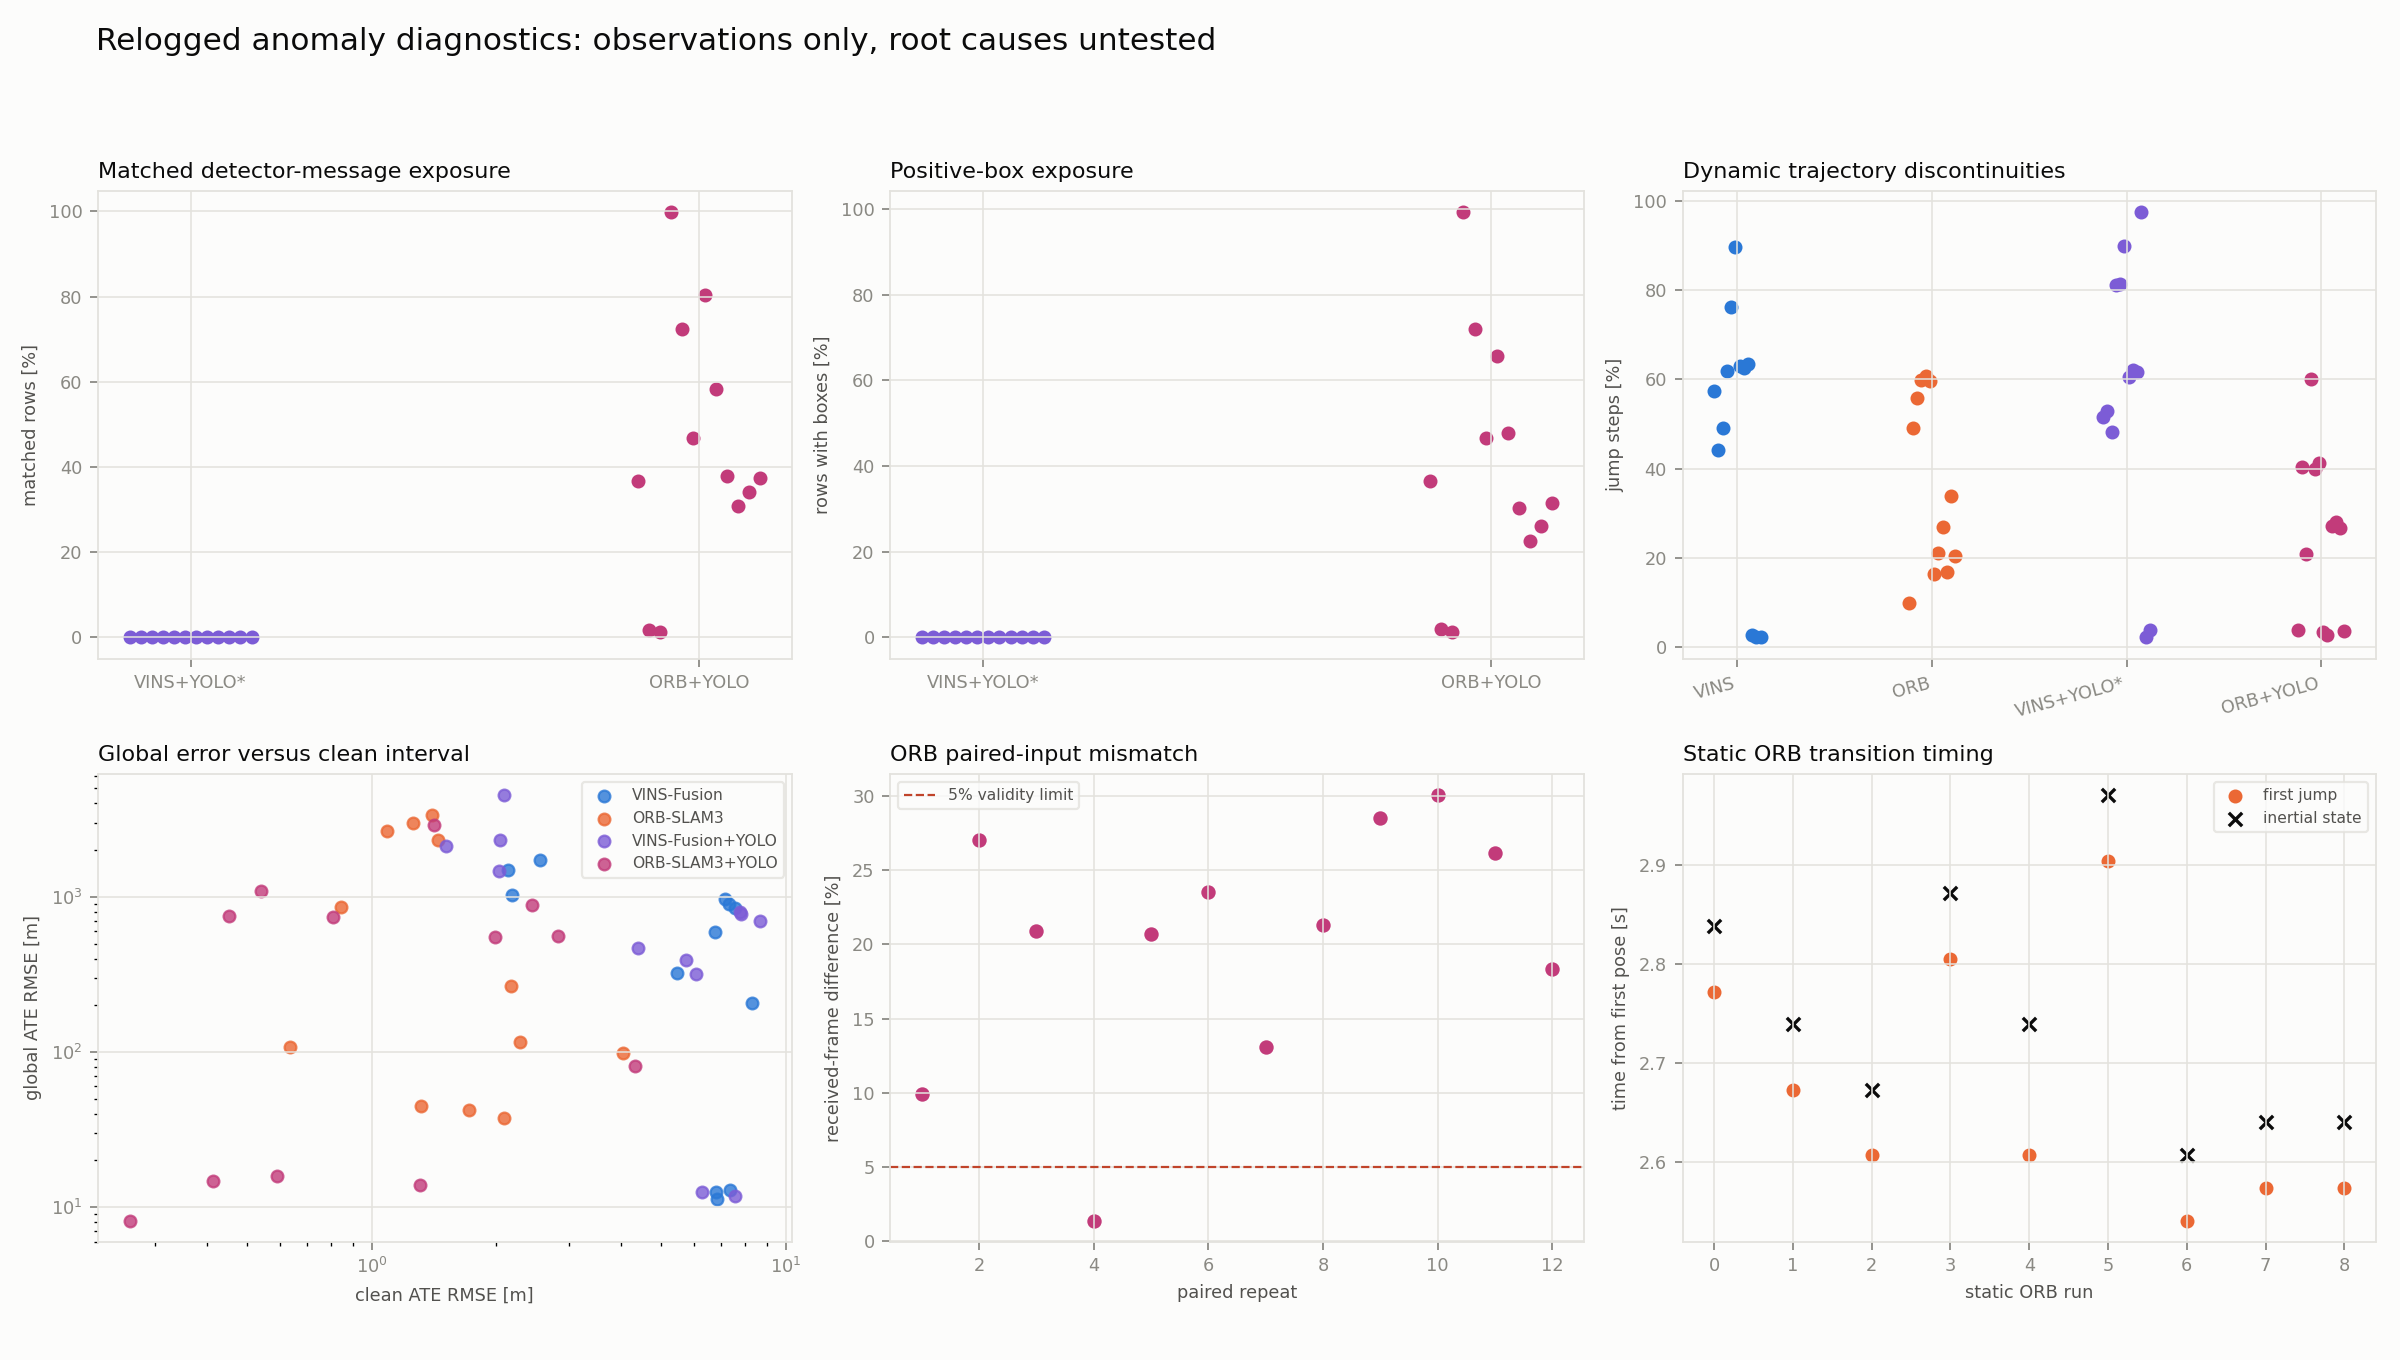
\includegraphics[width=\textwidth]{../../../output/compare/relogged_20260916/anomaly_diagnostics_light.png}
  \caption[Run-level anomaly diagnostics.]{Run-level anomaly diagnostics. The panels show detector-message and
  positive-box exposure, dynamic jump fractions, global versus clean-segment
  ATE, ORB paired-input mismatch, and static ORB jump timing. These are
  observations only; the plot does not assign a root cause.}
  \label{fig:anomaly-diagnostics}
\end{figure}


\subsubsection{Trajectory accuracy, plausibility and robustness}
\label{sec:trajectory-results}
% Verbatim from minor_report/chapters/chapter_4_results.tex lines 1115-1326 (retired report),
% headings demoted by 1 level(s). Do not edit here; edit the source of the numbers.

\begin{queried}[Excluded: dynamic-scene trajectory results]
Every dynamic-scene trajectory result in this section, and the anomalies A3 and
A4 that derive from them, are \textbf{withheld as findings} and retained only as
excluded evidence. The reason is the environment, not the measurement: the
dynamic worlds move their props along scripted kinematic paths. The props carry
collision geometry but produce no dynamic response against the robot, nothing
constrains their speeds or routes to warehouse traffic, and they can occupy the
same space as the vehicle without consequence. Numbers measured there describe
the simulation, not the problem the thesis poses.

The runs happened, the artifacts are intact, and the plausibility failures are
real properties of those recordings, so they are reported below rather than
deleted --- an excluded measurement that explains a methodological correction is
worth more in the record than a gap. What must not be done is to read them as
evidence about estimator behaviour in a dynamic warehouse.

Two consequences follow. The condition this work is named for currently has no
valid testbed: it is untested, not tested and failed. And the environment becomes
the leading candidate explanation for the breakdown itself, displacing the
open question left in \cref{sec:anomaly-catalogue} --- testable by rebuilding the
worlds with physically simulated props and re-running, which requires no change
to either estimator.

Unaffected: the static-scene results here, the estimator comparison of
\cref{sec:results-proprio}, the detector evaluation of
\cref{sec:yolo-performance} --- prop motion is kinematic, which changes contact
physics rather than appearance, so detectability and class assignment are
untouched --- and the map evaluation of \cref{sec:map-quality}.
\end{queried}

Table~\ref{tab:trajectory-errors} reports medians and IQRs because the dynamic-run
distributions are strongly skewed. In static scenes, VINS attained a median
translational ATE RMSE of \SI{0.370}{\metre} and rotational RMSE of
\SI{1.56}{\degree} over nine valid runs. The nine valid static ORB runs attained
\SI{0.454}{\metre} and \SI{17.92}{\degree}. The orientation difference is much
larger than the positional difference and must be retained as a separate result.
\Cref{sec:rpe} shows that it is produced almost entirely by one or two discrete
events per run rather than by continuously worse orientation tracking.

\begin{table}[htbp]
\centering
\caption[Trajectory error against rosbag ground truth, median (IQR).]{Trajectory error against rosbag ground truth, median (IQR). ``Clean'' is
ATE RMSE after independently aligning the longest segment without an implied
speed above \SI{10}{\metre\per\second}. Requested VINS+YOLO values are not
active-filter measurements.}
\label{tab:trajectory-errors}
\resizebox{\textwidth}{!}{%
\begin{tabular}{llrrrr}
\toprule
Scene & Requested mode & ATE RMSE (m) & Rotation RMSE (deg) & Clean ATE (m) & Jumps \\
\midrule
Static & VINS-Fusion & $0.370\;(0.063)$ & $1.56\;(0.98)$ & $0.370\;(0.063)$ & $0\;(0)$ \\
Static & ORB-SLAM3 & $0.454\;(0.157)$ & $17.92\;(1.72)$ & $0.341\;(0.151)$ & $1\;(1)$ \\
Dynamic & VINS-Fusion & $724.13\;(823.52)$ & $53.97\;(39.38)$ & $6.80\;(2.57)$ & $1116\;(1157.75)$ \\
Dynamic & ORB-SLAM3 & $190.48\;(2315.44)$ & $108.29\;(116.13)$ & $1.42\;(0.89)$ & $484\;(418.5)$ \\
Dynamic & VINS-Fusion+YOLO$^{*}$ & $738.63\;(1251.84)$ & $56.50\;(37.88)$ & $5.91\;(5.53)$ & $1559.5\;(717)$ \\
Dynamic & ORB-SLAM3+YOLO & $556.05\;(769.39)$ & $138.42\;(60.34)$ & $1.06\;(1.58)$ & $208\;(225.5)$ \\
\bottomrule
\multicolumn{6}{l}{$^{*}$Filter requested but no detection frame was matched.}
\end{tabular}}
\end{table}

Every dynamic run contains at least one impossible-speed step. Nine of 12
baseline VINS runs, all 12 baseline ORB runs, 10 of 12 nominal VINS+YOLO runs,
and all 12 ORB+YOLO runs also exceeded the reference-free mean-speed limit of
\SI{3}{\metre\per\second}. Peak translational error exceeded \SI{50}{\metre} in
9, 12, 10, and 10 runs respectively. Global ATE is therefore dominated by
trajectory breakdown. The clean-segment ATE is substantially smaller, which an
earlier draft read as evidence that the runs contain locally coherent intervals.
\Cref{sec:rpe} withdraws that reading: measured directly, the jump-free
relative error is \SIrange{1.8}{3.8}{\metre} per second, so the estimate is
locally wrong by more than the distance the robot travels. Aligning a short
segment absorbs much of that error, which is why clean-segment ATE looked
reassuring.

The per-repeat values behind those aggregates are given in
\cref{tab:truth-summary}.

\subsubsection{Relative pose error}
\label{sec:rpe}

RPE was implemented after the reporting cutoff and applied to the campaign
without re-running any estimator; \cref{sec:method-trajectory} defines it. It is
reported here because it needs no global alignment, so unlike ATE it cannot be
distorted by a single discontinuity re-seating the rigid fit.
\Cref{tab:rpe-summary} gives the headline interval.

\begin{table}[htbp]
\centering
\caption[Relative pose error at $\Delta=\SI{1}{\second}$, median (IQR) over runs.]{Relative pose error at $\Delta=\SI{1}{\second}$, median (IQR) over runs.
``Jump-free'' excludes pairs spanning a detected tracking jump; the difference
between the two columns is the teleport contribution. Requested VINS+YOLO values
are not active-filter measurements.}
\label{tab:rpe-summary}
\footnotesize
\setlength{\tabcolsep}{3pt}
% Generated by script/make_result_tables.py from
% output/compare/relogged_20260916/trajectory_metrics.csv.
% Do not edit by hand; regenerate instead.
\begin{tabular}{llrrrrr}
\toprule
& & & \multicolumn{2}{c}{Translational (m)} & \multicolumn{2}{c}{Rotational (deg)} \\
\cmidrule(lr){4-5}\cmidrule(lr){6-7}
Scene & Requested mode & Jumps & all pairs & jump-free & all pairs & jump-free \\
\midrule
Static & VINS-Fusion & 0\,(0) & 0.063\,(0.027) & 0.063\,(0.027) & 0.57\,(0.05) & 0.57\,(0.05) \\
Static & ORB-SLAM3 & 1\,(1) & 0.310\,(0.308) & 0.096\,(0.064) & 10.56\,(0.69) & 0.25\,(0.33) \\
\midrule
Dynamic & VINS-Fusion & 1116\,(1158) & 44.652\,(49.397) & 2.825\,(1.595) & 2.05\,(1.63) & 2.76\,(2.01) \\
Dynamic & ORB-SLAM3 & 484\,(418) & 19.477\,(158.567) & 2.079\,(0.267) & 15.15\,(4.82) & 2.49\,(2.51) \\
Dynamic & VINS-Fusion+YOLO$^{*}$ & 1560\,(717) & 44.106\,(95.564) & 3.784\,(1.611) & 2.33\,(4.76) & 2.72\,(1.02) \\
Dynamic & ORB-SLAM3+YOLO & 208\,(226) & 38.174\,(78.432) & 1.805\,(0.634) & 21.60\,(9.72) & 6.33\,(10.39) \\
\bottomrule
\end{tabular}

\end{table}

Two results follow, and the first corrects this chapter.

\paragraph{The dynamic runs are not locally coherent.} Excluding every pair that
spans a jump, dynamic translational RPE at $\Delta=\SI{1}{\second}$ is still
\SIrange{1.8}{3.8}{\metre}. The robot covers about \SI{1.4}{\metre} in that
second, so between teleports the estimate misstates its own motion by more than
the distance travelled. Against the static runs, whose jump-free figures are
\SIrange{0.063}{0.096}{\metre}, dynamic local error is \num{20} to \num{60}
times worse. The corruption is therefore continuous, not confined to isolated
steps, and the earlier reading of clean-segment ATE as evidence of local
coherence does not survive. This was a registered prediction before the metric
was run, and it failed in the direction that matters.

\begin{table}[htbp]
\centering
\caption[Jump-free translational RPE against interval, median over runs, in metres.]{Jump-free translational RPE against interval, median over runs, in
metres. ``Growth'' is the ratio from \SI{0.5}{\second} to \SI{5}{\second};
linear accumulation would give \num{10}$\times$ and a pure random walk
\num{3.2}$\times$.}
\label{tab:rpe-sweep}
\small
\setlength{\tabcolsep}{5pt}
% Generated by script/make_result_tables.py from
% output/compare/relogged_20260916/trajectory_metrics.csv.
% Do not edit by hand; regenerate instead.
\begin{tabular}{llrrrrr}
\toprule
Scene & Requested mode & \SI{0.5}{\second} & \SI{1.0}{\second} & \SI{2.0}{\second} & \SI{5.0}{\second} & Growth \\
\midrule
Static & VINS-Fusion & 0.038 & 0.063 & 0.112 & 0.252 & 6.7$\times$ \\
Static & ORB-SLAM3 & 0.057 & 0.096 & 0.162 & 0.307 & 5.4$\times$ \\
\midrule
Dynamic & VINS-Fusion & 1.524 & 2.825 & 5.067 & 10.082 & 6.6$\times$ \\
Dynamic & ORB-SLAM3 & 1.158 & 2.079 & 3.776 & 6.787 & 5.9$\times$ \\
Dynamic & VINS-Fusion+YOLO$^{*}$ & 2.189 & 3.784 & 5.455 & 10.985 & 5.0$\times$ \\
Dynamic & ORB-SLAM3+YOLO & 0.976 & 1.805 & 3.041 & 4.384 & 4.5$\times$ \\
\bottomrule
\end{tabular}

\end{table}

\Cref{tab:rpe-sweep} shows why this is one mechanism rather than two. Error grows
with interval at \numrange{4.5}{6.7}$\times$ over a tenfold increase in
$\Delta$, and that growth exponent is the same for static and dynamic scenes;
only the magnitude differs, by roughly \num{40}$\times$. The dynamic runs are
not failing in a qualitatively different way from the static ones --- they are
running the same error process far hotter.

\paragraph{ORB-SLAM3's static rotational penalty is entirely jump-localised.}
Static ORB-SLAM3 carries a rotational ATE of \SI{17.92}{\degree} against
VINS-Fusion's \SI{1.56}{\degree}, an elevenfold gap that invites the reading
that ORB-SLAM3 tracks orientation poorly. RPE refutes it. Across the nine static
ORB runs, all-pairs rotational RPE is \SIrange{9.28}{11.63}{\degree}, but
jump-free rotational RPE is \SIrange{0.10}{0.66}{\degree} --- at or below
VINS-Fusion's \SIrange{0.49}{0.69}{\degree} on the same recordings. Every one of
those runs contains one or two jumps and no more.

The whole rotational gap is thus produced by one or two discrete re-seating
events per run, not by continuously worse tracking. This gives anomaly~A5 its
significance: that jump occurs near \SI{2.6}{\second}, immediately before
inertial initialization completes, and it is predominantly rotational. Between
those events ORB-SLAM3's orientation tracking is competitive with VINS-Fusion's.
No causal mechanism is established here --- the association is temporal --- but
the error is now localized to an event rather than attributed to the estimator's
steady-state behaviour.

\begin{sidewaystable}[p]
\centering
\caption[Truth-based trajectory error for every repeat of the relogged campaign.]{Truth-based trajectory error for every repeat of the relogged
campaign. Every dataset is a no-floor-texture world, so that shared part of each
dataset name is omitted. ``ATE'' and ``clean'' are global and
longest-clean-segment ATE RMSE in metres, ``rot'' is rotational geodesic RMSE in
degrees, and ``jmp'' counts steps implying more than \SI{10}{\metre\per\second}.
All 66 runs are operational; two static ORB run summaries have incomplete
schemas, and only one of 12 ORB baseline/filter pairs passed input matching.
Static datasets were not run in either filtered mode; those cells are set to --.}
\label{tab:truth-summary}
\scriptsize
\setlength{\tabcolsep}{4pt}
% Generated by script/make_result_tables.py from
% output/compare/relogged_20260916/trajectory_metrics.csv.
% Do not edit by hand; regenerate instead.
\begin{tabular}{llrrrrrrrrrrrrrrrr}
\toprule
& & \multicolumn{4}{c}{VINS-Fusion} & \multicolumn{4}{c}{ORB-SLAM3} & \multicolumn{4}{c}{VINS-Fusion+YOLO$^{*}$} & \multicolumn{4}{c}{ORB-SLAM3+YOLO} \\
\cmidrule(lr){3-6}\cmidrule(lr){7-10}\cmidrule(lr){11-14}\cmidrule(lr){15-18}
Dataset & Rep & ATE & rot & clean & jmp & ATE & rot & clean & jmp & ATE & rot & clean & jmp & ATE & rot & clean & jmp \\
& & (m) & (deg) & (m) & (n) & (m) & (deg) & (m) & (n) & (m) & (deg) & (m) & (n) & (m) & (deg) & (m) & (n) \\
\midrule
dynamic 00\_000 & 01 & 596.37 & 38.5 & 6.77 & 858 & 45.21 & 176.5 & 1.31 & 109 & 392.55 & 107.0 & 5.74 & 1122 & 13.84 & 76.7 & 1.31 & 37 \\
dynamic 00\_000 & 02 & 206.97 & 92.2 & 8.32 & 609 & 857.95 & 162.0 & 0.84 & 512 & 466.72 & 108.0 & 4.39 & 1183 & 892.31 & 129.9 & 2.45 & 213 \\
dynamic 00\_000 & 03 & 324.01 & 88.4 & 5.47 & 580 & 3364.34 & 70.8 & 1.40 & 610 & 318.66 & 108.7 & 6.07 & 991 & 81.20 & 173.1 & 4.33 & 119 \\
dynamic 00\_001 & 01 & 1030.40 & 63.6 & 2.18 & 1374 & 3002.57 & 29.7 & 1.26 & 1150 & 2309.93 & 74.6 & 2.04 & 1805 & 2885.77 & 82.2 & 1.42 & 1159 \\
dynamic 00\_001 & 02 & 1481.00 & 62.8 & 2.14 & 1695 & 2669.73 & 26.1 & 1.09 & 1141 & 2129.97 & 75.2 & 1.51 & 1810 & 553.35 & 93.5 & 1.98 & 454 \\
dynamic 00\_001 & 03 & 1724.94 & 175.1 & 2.55 & 1995 & 2311.30 & 23.1 & 1.45 & 1098 & 1457.89 & 59.6 & 2.03 & 1997 & 558.76 & 112.8 & 2.82 & 378 \\
dynamic 01\_000 & 01 & 904.94 & 53.3 & 7.29 & 1608 & 98.88 & 169.1 & 4.05 & 239 & 698.15 & 52.0 & 8.67 & 1545 & 8.20 & 102.3 & 0.26 & 44 \\
dynamic 01\_000 & 02 & 851.90 & 53.8 & 7.55 & 1596 & 115.45 & 172.4 & 2.28 & 327 & 796.03 & 52.6 & 7.77 & 1582 & 14.78 & 173.8 & 0.41 & 26 \\
dynamic 01\_000 & 03 & 965.82 & 54.1 & 7.14 & 1619 & 107.60 & 167.7 & 0.64 & 456 & 779.10 & 53.3 & 7.79 & 1574 & 749.16 & 162.6 & 0.45 & 203 \\
dynamic 02\_000 & 01 & 12.49 & 6.1 & 6.80 & 72 & 37.83 & 59.3 & 2.09 & 388 & 4518.77 & 25.1 & 2.09 & 2610 & 1097.95 & 159.7 & 0.54 & 231 \\
dynamic 02\_000 & 02 & 12.88 & 5.5 & 7.36 & 61 & 265.50 & 62.9 & 2.17 & 689 & 11.85 & 6.4 & 7.55 & 62 & 737.27 & 148.9 & 0.81 & 219 \\
dynamic 02\_000 & 03 & 11.30 & 4.3 & 6.81 & 58 & 42.37 & 145.8 & 1.72 & 408 & 12.55 & 6.9 & 6.29 & 66 & 15.81 & 146.9 & 0.59 & 31 \\
\midrule
static 000 & 01 & 0.37 & 1.6 & 0.37 & 0 & 0.58 & 17.9 & 0.55 & 1 & -- & -- & -- & -- & -- & -- & -- & -- \\
static 000 & 02 & 0.41 & 1.5 & 0.41 & 0 & 0.79 & 20.4 & 0.77 & 1 & -- & -- & -- & -- & -- & -- & -- & -- \\
static 000 & 03 & 0.43 & 1.6 & 0.43 & 0 & 1.20 & 19.1 & 0.30 & 2 & -- & -- & -- & -- & -- & -- & -- & -- \\
static 001 & 01 & 0.39 & 2.3 & 0.39 & 0 & 0.45 & 18.9 & 0.27 & 2 & -- & -- & -- & -- & -- & -- & -- & -- \\
static 001 & 02 & 0.29 & 1.8 & 0.29 & 0 & 0.45 & 18.1 & 0.21 & 2 & -- & -- & -- & -- & -- & -- & -- & -- \\
static 001 & 03 & 0.48 & 2.2 & 0.48 & 0 & 0.38 & 17.2 & 0.26 & 1 & -- & -- & -- & -- & -- & -- & -- & -- \\
static 002 & 01 & 0.34 & 0.8 & 0.34 & 0 & 0.42 & 16.7 & 0.39 & 1 & -- & -- & -- & -- & -- & -- & -- & -- \\
static 002 & 02 & 0.36 & 0.8 & 0.36 & 0 & 0.46 & 17.6 & 0.43 & 1 & -- & -- & -- & -- & -- & -- & -- & -- \\
static 002 & 03 & 0.34 & 0.7 & 0.34 & 0 & 0.36 & 16.9 & 0.34 & 1 & -- & -- & -- & -- & -- & -- & -- & -- \\
\bottomrule
\end{tabular}


\vspace{1ex}
\raggedright\footnotesize
$^{*}$Filter requested but no detection frame was matched in any repeat; these
columns are not active-filter measurements.
\end{sidewaystable}

\begin{figure}[htbp]
  \centering
  % The summary table belongs with these panels, so it is set inside the float
  % rather than as a separate table that page-breaking could carry away.
  {\small\setlength{\tabcolsep}{3pt}% Generated by script/make_result_tables.py from
% output/compare/relogged_20260916/trajectory_metrics.csv.
% Do not edit by hand; regenerate instead.
\begin{tabular}{lrrrrrrr}
\toprule
Requested mode & Poses & Overlap & Path & ATE RMSE & Rot RMSE & Clean ATE & Jumps \\
& (n) & (s) & (m) & (m) & (deg) & (m) & (n) \\
\midrule
VINS-Fusion & 1494 & 77.0 & 5486.93 & 596.367 & 38.51 & 6.771 & 858 \\
ORB-SLAM3 & 1105 & 77.3 & 408.22 & 45.206 & 176.53 & 1.314 & 109 \\
VINS-Fusion+YOLO$^{*}$ & 2175 & 77.1 & 1958.14 & 392.546 & 107.04 & 5.743 & 1122 \\
ORB-SLAM3+YOLO & 943 & 77.2 & 239.53 & 13.839 & 76.72 & 1.310 & 37 \\
\bottomrule
\end{tabular}
}

  \vspace{0.5ex}
  {\footnotesize $^{*}$Filter requested but no detection frame was matched.}

  \vspace{2ex}
  % The image carries its own rendered title, the same summary table, and a
  % footnote in the top 310 px of 2496; that band is trimmed away because those
  % numbers are now typeset above.
  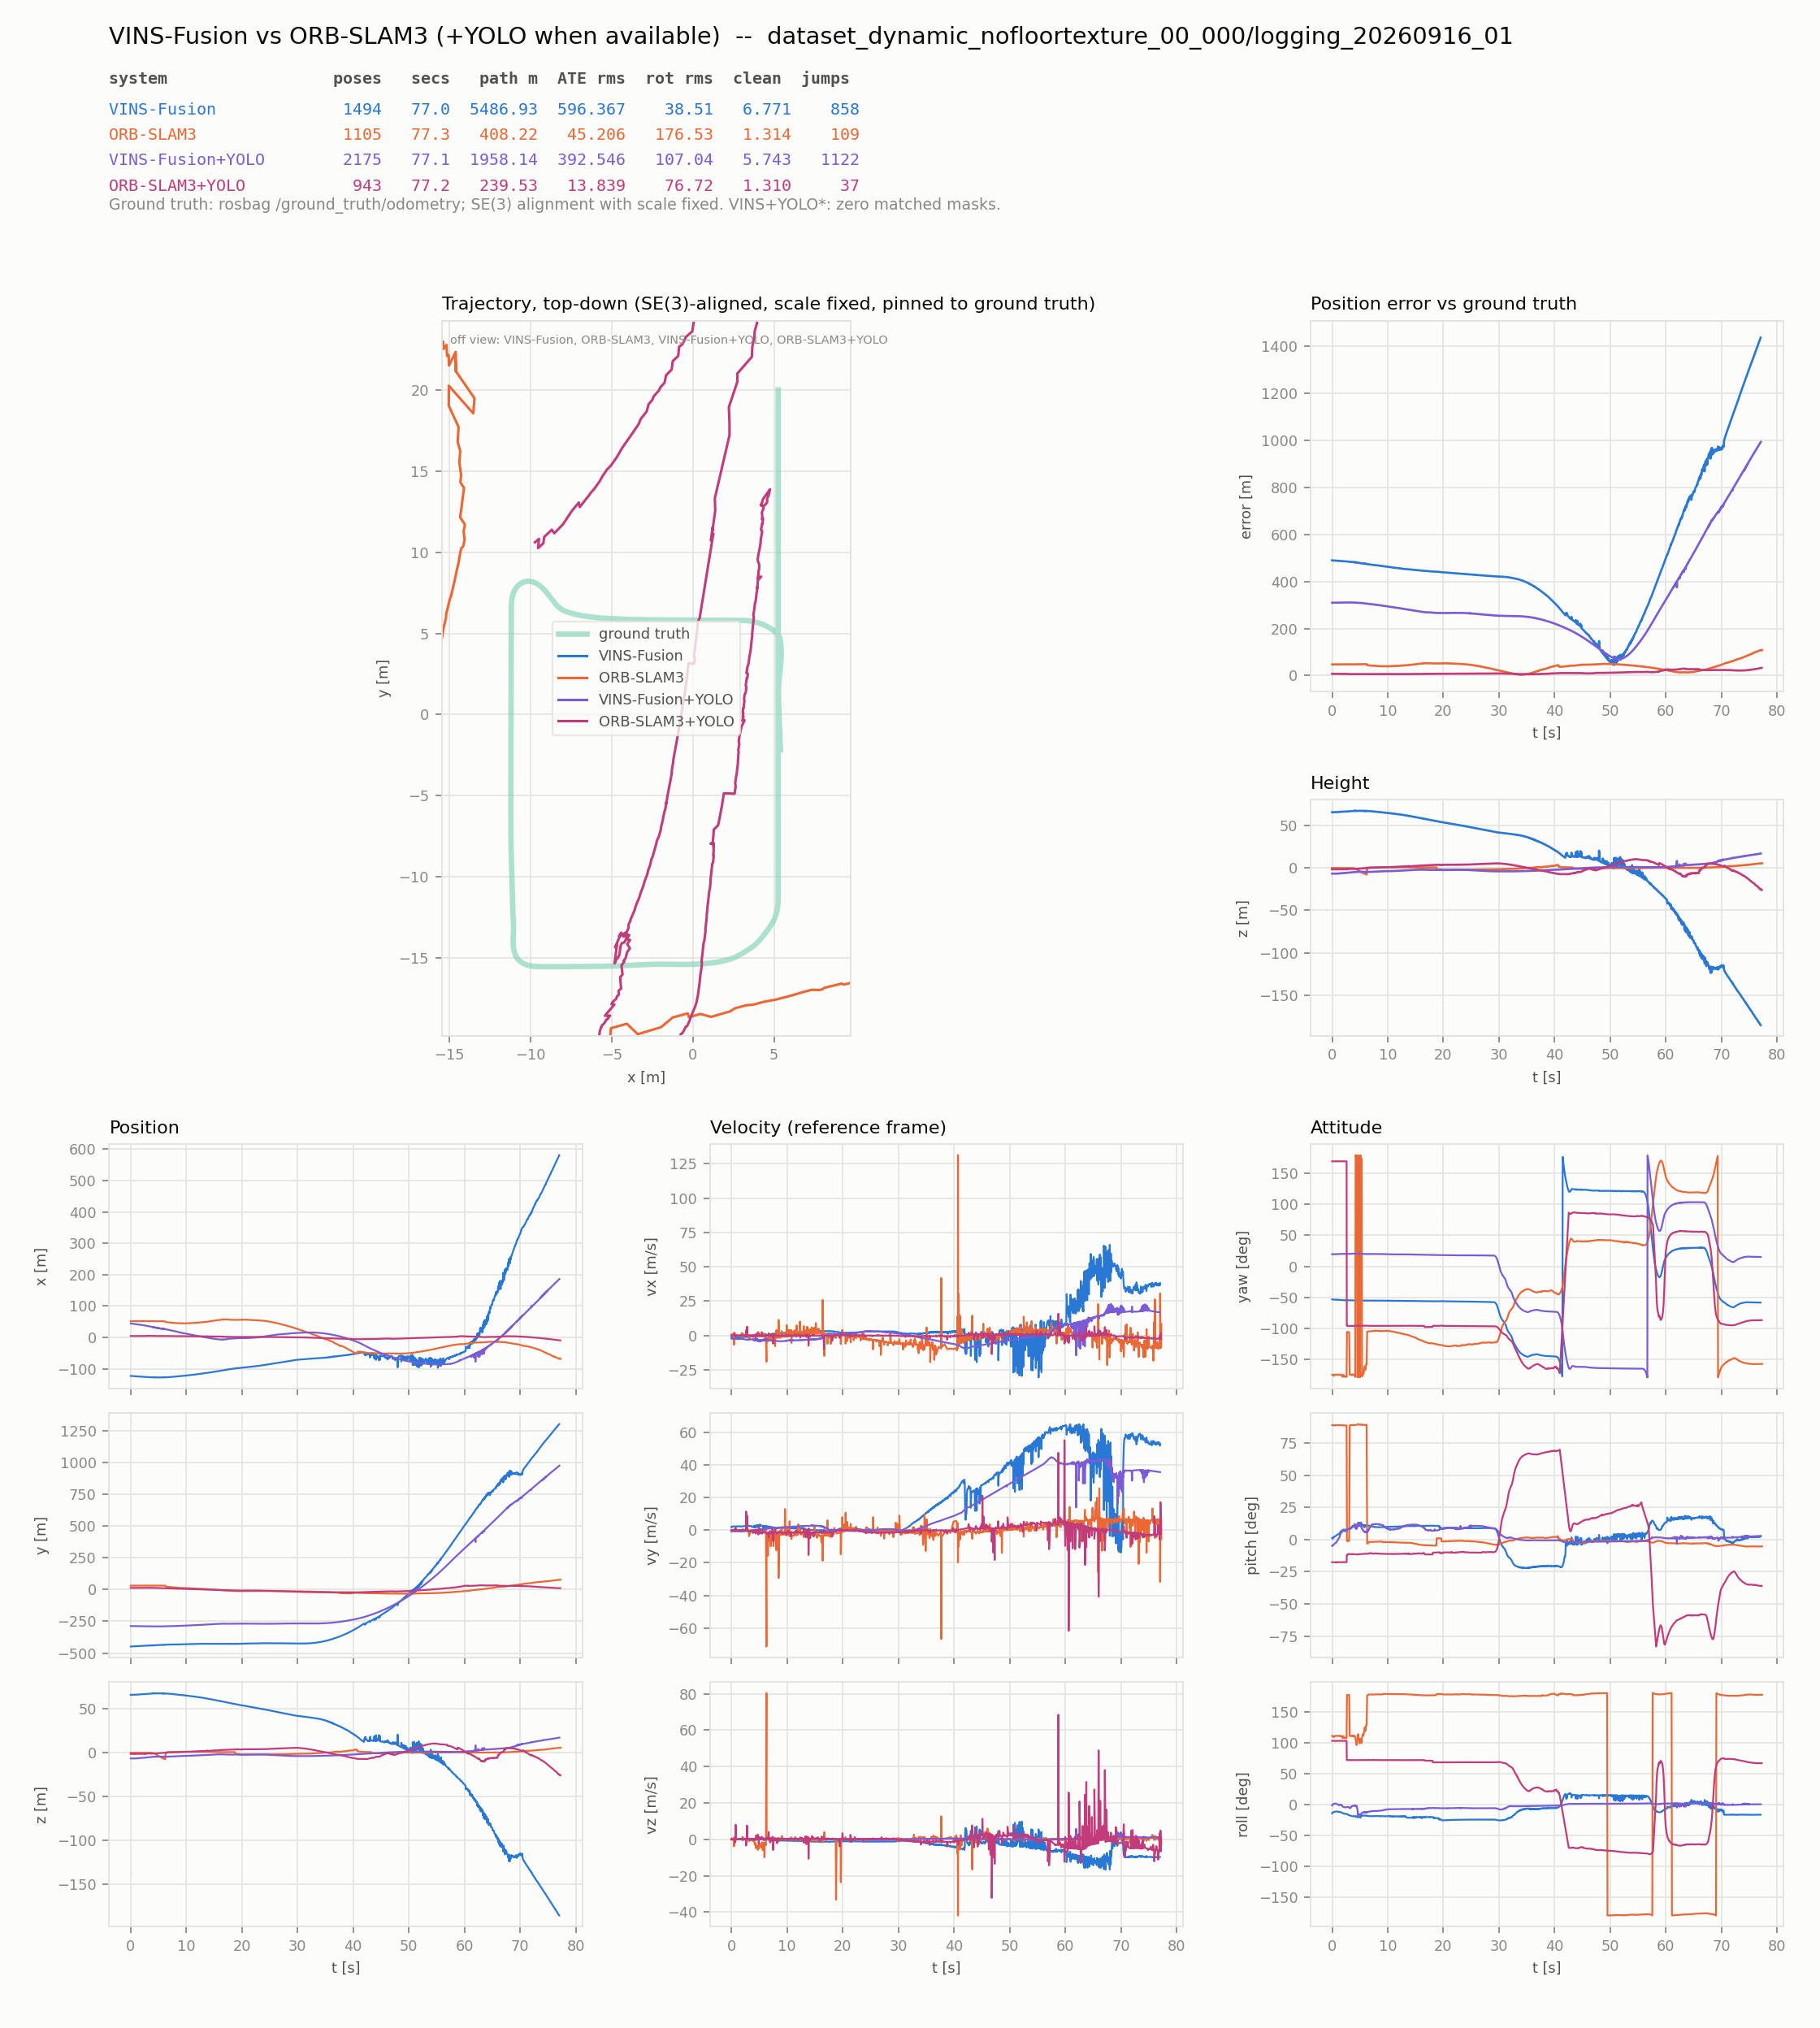
\includegraphics[width=\textwidth, trim={0 0 0 140pt}, clip]{../../../output/compare/relogged_20260916/simulation/dataset_dynamic_nofloortexture_00_000/logging_20260916_01/compare_light.png}
  \caption[Representative repeated-run trajectory diagnostic for \repo{dataset_dynamic_nofloortexture_00_000/logging_20260916_01}, in the same visual format as the existing comparison figures.]{Representative repeated-run trajectory diagnostic for
  \repo{dataset_dynamic_nofloortexture_00_000/logging_20260916_01}, in the same
  visual format as the existing comparison figures. The table gives the
  per-system summary for this run; ``clean'' is ATE RMSE over the longest
  jump-free segment. The very large paths and frequent jumps are retained rather
  than clipped into a favourable view. ATE and rotational errors use the rosbag
  \repo{/ground_truth/odometry} topic after rigid $SE(3)$ alignment with scale
  fixed. The nominal VINS+YOLO trace is invalid as a filtering treatment because
  no masks were matched.}
  \label{fig:relogged-trajectory-example}
\end{figure}

Baseline ORB-SLAM3 logged $7.75\pm6.03$ tracking-loss events and
$9.52\pm6.49$~s of lost tracking per dynamic run (mean $\pm$ sample SD,
$n=12$). ORB+YOLO logged $9.17\pm3.01$ events and $11.46\pm5.32$~s. VINS logged
no estimator resets in either requested mode, but the absence of resets does not
make its trajectories plausible. The event types are estimator-specific and are
not treated as numerically equivalent.

\begin{figure}[htbp]
  \centering
  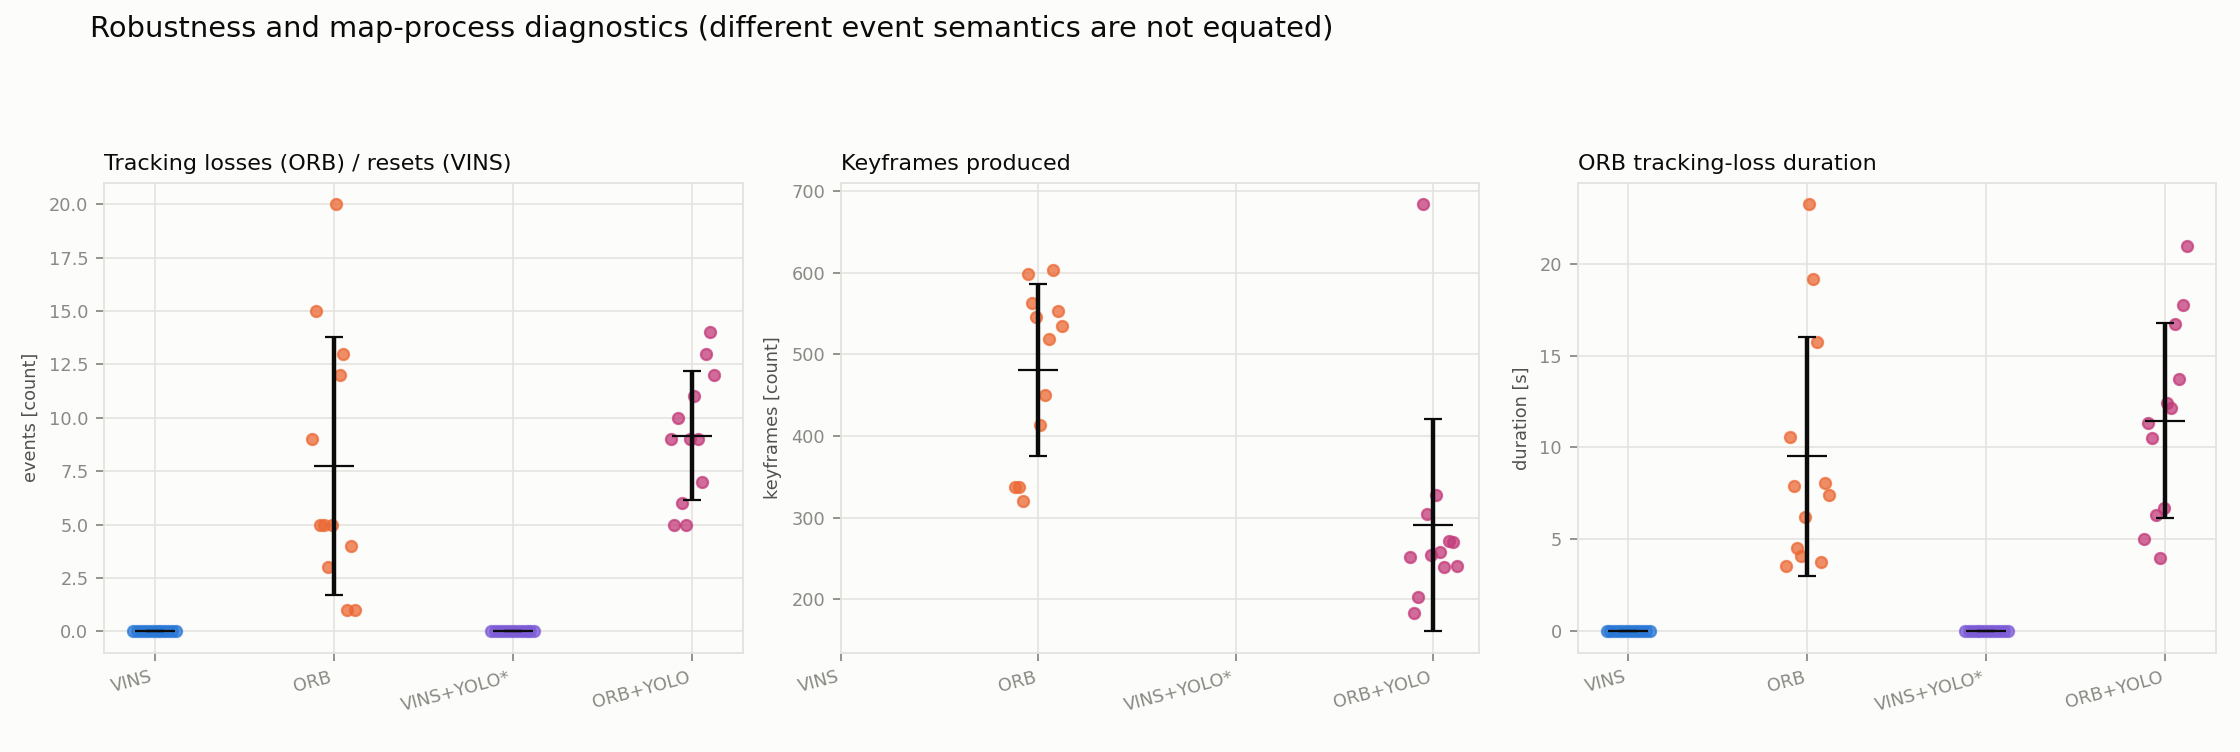
\includegraphics[width=\textwidth]{../../../output/compare/relogged_20260916/robustness_light.png}
  \caption[Per-run robustness and keyframe observations for the dynamic datasets.]{Per-run robustness and keyframe observations for the dynamic datasets.
  Points are experimental runs and black marks are mean $\pm$ sample SD. VINS
  reset count and ORB tracking-loss count have different semantics. The asterisk
  identifies the requested VINS filter mode in which no masks were matched.}
  \label{fig:robustness-results}
\end{figure}


\subsubsection{Real-time and computational measurements}
\label{sec:compute-results}
% Verbatim from minor_report/chapters/chapter_4_results.tex lines 1331-1393 (retired report),
% headings demoted by 0 level(s). Do not edit here; edit the source of the numbers.

Table~\ref{tab:capacity-results} summarizes process-local measurements over the
12 dynamic runs in each requested mode. CPU is the change in cumulative process
CPU time divided by monotonic wall time; 100\% denotes one fully used logical
core, so values above 100\% represent multithreaded execution. Memory is peak
resident set size. The separate detector process, rosbag, Gazebo, RViz, and
RTAB-Map are not included.

\begin{table}[htbp]
\centering
\caption[Dynamic-run capacity and resource measurements, mean $\pm$ sample SD, $n=12$ per row.]{Dynamic-run capacity and resource measurements, mean $\pm$ sample SD,
$n=12$ per row. Nominal VINS+YOLO values are not active-filter measurements.}
\label{tab:capacity-results}
\resizebox{\textwidth}{!}{%
\begin{tabular}{lrrrr}
\toprule
Requested mode & Throughput (Hz) & Retained input (\%) & CPU (\% core) & Peak RSS (MiB) \\
\midrule
VINS-Fusion & $27.14\pm5.81$ & $100.00\pm0.00$ & $443.66\pm58.96$ & $629.51\pm282.62$ \\
ORB-SLAM3 & $23.47\pm4.77$ & $88.55\pm13.42$ & $385.22\pm27.71$ & $1226.06\pm81.83$ \\
VINS-Fusion+YOLO$^{*}$ & $28.83\pm3.16$ & $100.00\pm0.00$ & $406.43\pm89.95$ & $646.14\pm306.15$ \\
ORB-SLAM3+YOLO & $14.47\pm5.42$ & $66.96\pm15.26$ & $410.86\pm42.83$ & $1054.64\pm91.11$ \\
\bottomrule
\multicolumn{5}{l}{$^{*}$Filter requested but no detection frame was matched.}
\end{tabular}}
\end{table}

The ORB+YOLO folders show lower achieved throughput and retention than baseline
ORB, while process CPU is of similar order. This is an observation, not an
isolated detector-cost effect: the external detector is excluded from CPU and 11
paired runs received materially different image counts. Baseline VINS processed
all enqueued images in its logs, whereas baseline ORB discarded frames whenever
the one-frame queue was overwritten.

\begin{figure}[htbp]
  \centering
  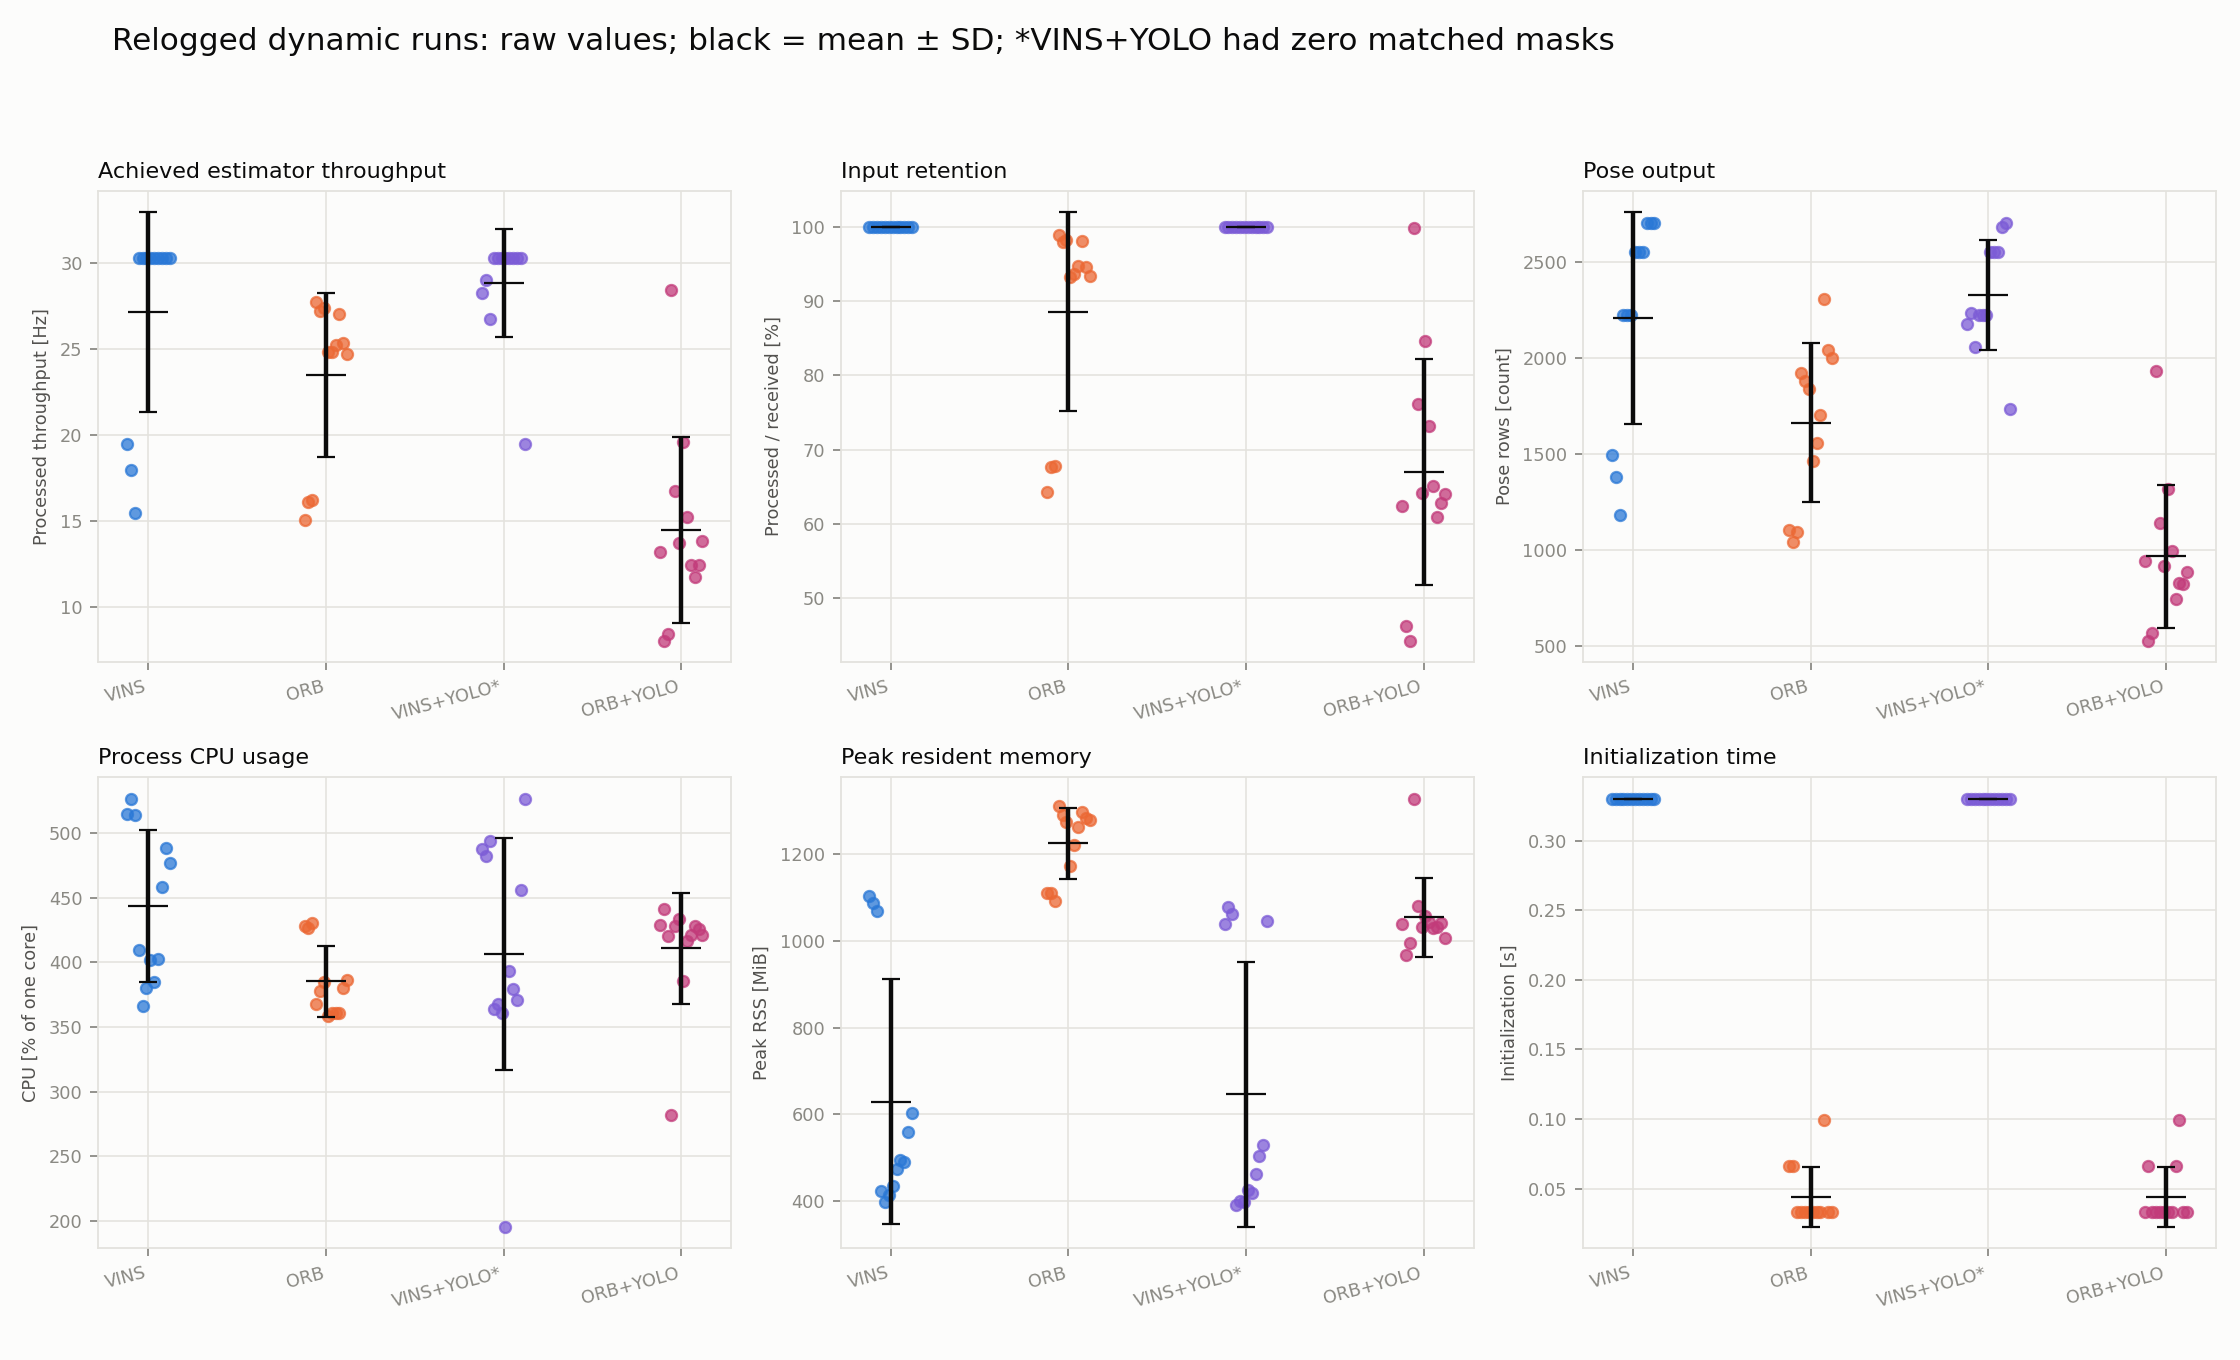
\includegraphics[width=\textwidth]{../../../output/compare/relogged_20260916/capacity_resources_light.png}
  \caption[Raw dynamic-run capacity and process-resource values.]{Raw dynamic-run capacity and process-resource values. Each point is a
  run; black marks show mean $\pm$ sample SD. This plot exposes run-to-run spread
  rather than presenting only aggregate bars.}
  \label{fig:capacity-resources}
\end{figure}

Per-module results use each run's event distribution. Figure~\ref{fig:module-latency}
shows pooled event boxplots for shape, overlaid with one median point per run so
frames are not mistaken for independent experimental repeats. Across run medians,
ORB tracking was $63.19\pm7.06$~ms and ORB local mapping was
$189.58\pm16.95$~ms. The requested ORB+YOLO mode measured
$112.53\pm24.61$~ms and $356.30\pm68.36$~ms respectively. VINS feature tracking
was $48.00\pm10.83$~ms and its back end was $60.41\pm17.12$~ms; nominal
VINS+YOLO values were $43.61\pm11.49$~ms and $57.90\pm16.29$~ms, but cannot be
interpreted as filter effects because that filter was inactive. These timings
refer to different estimator stages and are not added or treated as directly
equivalent algorithms.

\begin{figure}[htbp]
  \centering
  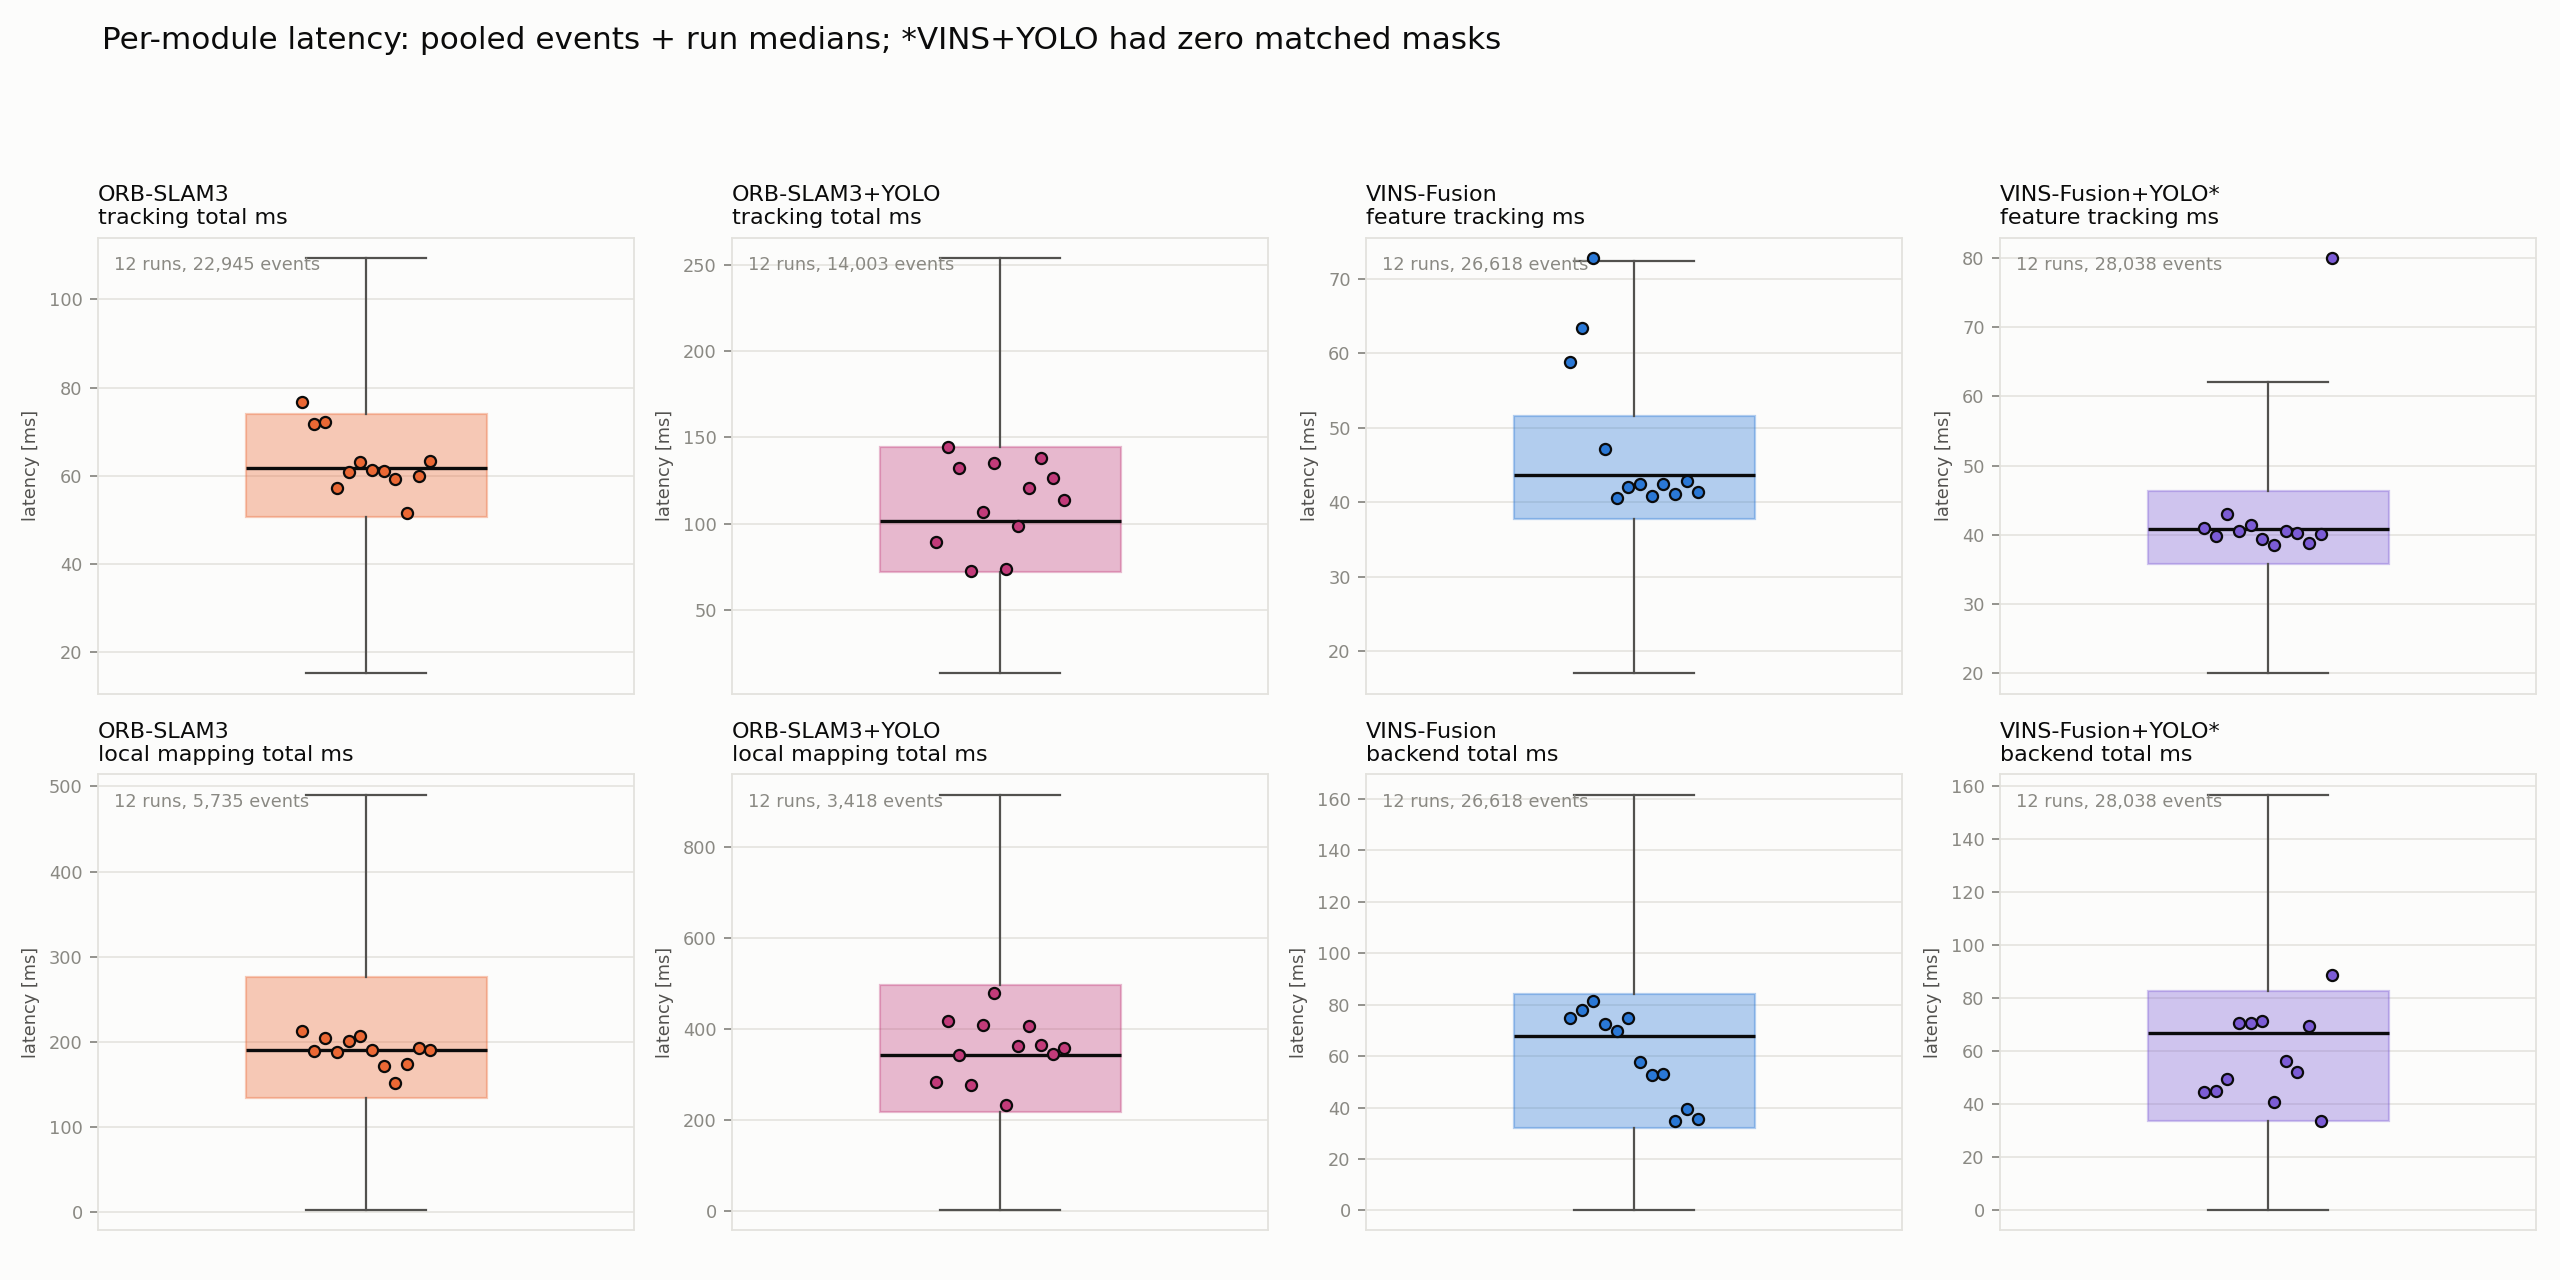
\includegraphics[width=\textwidth]{../../../output/compare/relogged_20260916/module_latency_light.png}
  \caption[Module-latency distributions for dynamic datasets.]{Module-latency distributions for dynamic datasets. Boxes summarize
  all recorded module events; coloured points are per-run medians ($n=12$ in
  each requested mode). ORB local mapping is asynchronous per keyframe, while
  VINS back-end rows follow estimator updates.}
  \label{fig:module-latency}
\end{figure}


\subsubsection{Loop closure, map merging and global-correction evidence}
\label{sec:global-events}
% Verbatim from minor_report/chapters/chapter_4_results.tex lines 1712-1724 (retired report),
% headings demoted by 0 level(s). Do not edit here; edit the source of the numbers.

The expanded ORB logs now expose back-end events. Baseline ORB-SLAM3 recorded six
loop closures: two in each repeat of
\repo{dataset_static_nofloortexture_002}. Each of those runs also recorded two
global bundle-adjustment executions. One baseline dynamic run
(\repo{dataset_dynamic_nofloortexture_02_000/logging_20260916_03}) and one
ORB+YOLO run
(\repo{dataset_dynamic_nofloortexture_01_000/logging_20260916_02}) recorded a map
merge. These counters demonstrate that the native ORB back-end paths executed;
they do not demonstrate that the resulting corrections were correct. The
failed trajectory-plausibility checks and the absence of an event-aligned
before/after counterfactual prevent a correction-benefit claim. RTAB-Map reconstruction remains a separate pipeline and is not exercised by
this relogged campaign; its dense-map evidence is reported independently in
\cref{sec:map-quality}, on a different world and database.


\paragraph{Summary.} In static scenes the two front ends reach a median aligned
ATE of \SI{0.370}{\metre} (VINS-Fusion) and \SI{0.454}{\metre} (ORB-SLAM3), and
ORB-SLAM3's large rotational error is produced by one or two discrete
initialisation-adjacent jumps rather than by its steady-state tracking. The
dynamic-scene numbers are withheld as findings: every dynamic trajectory is
locally wrong by more than the distance the robot travels, and the environment
that produced them is not physical. The core hypothesis therefore has no valid
test yet, and neither pipeline processes frames as fast as they arrive at the
replay rate used.

\paragraph{Future plan.} Fix the detection-to-VINS integration so that masked
tracks are actually culled, verified by the removed-track counter before any
re-run; reduce ORB-SLAM3+YOLO26 latency so that filtered and unfiltered runs see
the same frames; and rebuild the dynamic worlds with physically simulated props.

\subsection{Real robot}
\label{sec:exp3-real}

\slotstatus{blocked}{Real-robot trajectory accuracy cannot be claimed at the
cutoff: the rig's IMU-to-camera translation is a zero placeholder, the second
camera reuses the first camera's intrinsics, and no recording carries an
independent ground truth (\cref{tab:real-rig,tab:deviations}).}

\textbf{Reason.} The three calibration gaps of \cref{sec:real-calibration}
bound what any real run can show to plausibility and tracking continuity;
metric ATE and RPE need the motion-capture reference of \cref{sec:real-site},
which has not been recorded. Runs on \repo{dataset_real_000} are consequently
not reported here as results.

\textbf{Next action.} Complete the camera--IMU calibration (extrinsic
translation, per-camera intrinsics), record the motion-capture trajectory, then
execute the four-step online procedure of \cref{sec:vio-filter-method} for both
pipelines at the three illumination levels, at
\SI{1.5}{\metre\per\second}, with the dynamic variable triggered at each zone
transfer.

% =====================================================================
\section{Experiment 4: Dense Map Reconstruction and Map-Quality Evaluation}
\label{sec:exp4}

\subsection{Simulation}
\label{sec:map-quality}

\slotstatus{partial}{One database, the tiny warehouse, is scored for geometry
and drivability. The large-warehouse map attempt failed through tracking loss
and produced no scorable database.}

\textbf{Objective.} Verify that the reconstructed map reflects the physical
environment and is usable by a planner (\cref{sec:map-eval-method}).

\textbf{Process.} RTAB-Map 0.23.7 built \repo{map/map_tiny.db}; its placement
was measured by \repo{script/fit_map_pose.py}; geometry and drivability were
scored by \repo{script/validate_map.py} against the world file and a
ground-truth route.

\textbf{Dataset.} \repo{dataset_map_tiny} (the build run) and the independent
route \repo{dataset_static_tiny_repeat}, which no longer exists; and, for the
large warehouse, \repo{dataset_map_01} (\cref{tab:dataset-registry}).

% Verbatim from minor_report/chapters/chapter_4_results.tex lines 1399-1707 (retired report),
% headings demoted by 1 level(s). Do not edit here; edit the source of the numbers.

\subsubsection{Question, scope, and conditions}

Trajectory error answers whether the robot knew where it was. It does not answer
whether the map it produced describes the building, nor whether a planner could
have used that map. This section evaluates the one dense map reconstructed so far
against two references of very different strength: the simulator's own collision
geometry, which is independent of the map, and the ground-truth route of the run
that built the map, which is not. The two questions are kept separate because
they fail in different ways --- a map can be geometrically faithful and still
unusable, and it can be navigable over an easy route while misrepresenting the
parts of the building that route never entered --- and because only the first
reference is independent evidence.

The evaluation is confined to the \textbf{tiny} warehouse. A large-warehouse
equivalent is \status{planned}; no database for it exists at the reporting
cutoff. Tiny-map and large-map results must not be pooled or read as repeated
trials of one condition, because the two worlds differ in extent, aisle width,
and route length. \Cref{tab:map-conditions} records the conditions.

\begin{table}[htbp]
\centering
\caption[Conditions for the dense-map evaluation.]{Conditions for the dense-map evaluation. The database and the
ground-truth route come from the \emph{same} run, which bounds what the
drivability figures can establish.}
\label{tab:map-conditions}
\small
\begin{tabularx}{\textwidth}{>{\raggedright\arraybackslash}p{0.26\textwidth}>{\raggedright\arraybackslash}X}
\toprule
Factor & Level \\
\midrule
Map under test & \repo{map/map_tiny.db}, RTAB-Map 0.23.7, created 2026-09-08 \\
World &
  \repo{aws-robomaker-small-warehouse-world/worlds/small_warehouse_static/small_warehouse_static_tinymap.world}
  (tiny geometry, despite residing in the \repo{small_warehouse_static} family
  directory) \\
Scene dynamics & static \\
Grid resolution & \SI{0.05}{\metre} \\
Geometry tolerance & \SI{0.25}{\metre} \\
Robot footprint & $0.83\times0.50$~m rectangle from
  \repo{nav2_ackermann.yaml}, not a circumscribed radius \\
World-to-map placement & $x=\SI{1.850}{\metre}$, $y=\SI{8.600}{\metre}$,
  $\theta=\SI{-89.90}{\degree}$, measured once by \repo{script/fit_map_pose.py} \\
Drivability reference, as plotted & \repo{dataset_static_tiny_repeat},
  \num{2973} poses; an independent run, no longer present in the workspace or on
  the removable drive \\
Substitute available & \repo{dataset/dataset_map_tiny},
  \repo{/ground_truth/odometry}: \num{3032} messages over \SI{60.6}{\second} of
  simulation time. This is the run that \emph{built} the map, so it is not an
  equivalent replacement \\
Evaluator & \repo{script/validate_map.py} \\
Experimental unit, $n$ & one database; $n=1$ \\
\bottomrule
\end{tabularx}
\end{table}

\subsubsection{Map placement as a validity precondition}
\label{sec:map-placement}

Both metrics depend on seating the occupancy grid in world coordinates, so
placement is a precondition rather than a display choice: a mis-seated grid
scores real structure against the wrong cells and makes a good map look bad. The
transform is a constant for a given database and is measured once, by fitting
occupied cells to the world file's wall and obstacle edges without using odometry
or ground truth. It is deliberately not taken from the live
\texttt{map~$\rightarrow$~odom} correction, which moves with front-end drift.

The measured fit is $(1.850, 8.600)\,\si{\metre}$ at \SI{-89.90}{\degree}, with a
margin of \SI{60.9}{\percent} over the best rival orientation more than
\SI{5}{\degree} away. An independent prediction --- the spawn pose of the IMU body
frame, which sits \SI{0.338}{\metre} ahead of \texttt{base\_footprint} --- gives
$(1.800, 8.662)\,\si{\metre}$. The two agree to \SI{0.080}{\metre}, inside the
grid's own \SI{0.05}{\metre} resolution. Two independent routes to the same
number is what makes this a measurement rather than a tuned parameter.

\subsubsection{Graph and database summary}

\Cref{tab:map-graph} summarizes the stored graph, read directly from the database
in read-only mode. The counts are small: \num{30} nodes over a \SI{59.3}{\second}
span, reflecting RTAB-Map's retention policy rather than the rate at which images
were offered to it.

\begin{table}[htbp]
\centering
\caption[Stored contents of \repo{map/map_tiny.db}.]{Stored contents of \repo{map/map_tiny.db}. Link rows are stored per
direction; the undirected count is the number of distinct node pairs.}
\label{tab:map-graph}
\small
\begin{tabularx}{\textwidth}{>{\raggedright\arraybackslash}p{0.30\textwidth}rr>{\raggedright\arraybackslash}X}
\toprule
Element & Rows & Undirected & Note \\
\midrule
Nodes & 30 & -- & ids 1--30, stamp span \SI{59.3}{\second} \\
Neighbour links & 56 & 28 & sequential odometry constraints \\
Global loop closures & 5 & 3 & pairs $(9,22)$, $(10,23)$, $(29,30)$ \\
Gravity links & 30 & 30 & one per node \\
Local-space links & 0 & 0 & none recorded \\
Visual words & \num{10357} & -- & vocabulary size \\
Features & \num{28374} & -- & stored keypoints \\
\bottomrule
\end{tabularx}
\end{table}

Of the three distinct closure pairs, $(9,22)$ and $(10,23)$ join nodes roughly
half a lap apart and are genuine revisits of an earlier place. The third,
$(29,30)$, joins consecutive nodes and is therefore not a revisit; it should not
be counted as evidence of place recognition.

\subsubsection{Geometry against the world file}

Geometry is scored against the rasterized collision geometry of the world file at
a \SI{0.25}{\metre} tolerance. Recall is measured against \emph{surfaces} rather
than filled interiors, because a stereo camera can only observe the outside of a
shelf; counting its interior as missed geometry would cap even a perfect map well
below \SI{100}{\percent}.

\begin{table}[htbp]
\centering
\caption{Occupied-cell geometry of \repo{map/map_tiny.db} against
\repo{small_warehouse_static_tinymap.world} at \SI{0.25}{\metre} tolerance.}
\label{tab:map-geometry}
\small
\begin{tabularx}{\textwidth}{>{\raggedright\arraybackslash}p{0.34\textwidth}r>{\raggedright\arraybackslash}X}
\toprule
Metric & Value & Population \\
\midrule
Occupied-cell precision & \SI{96.6}{\percent} & \num{11634} occupied cells \\
Recall, region the map observed & \SI{89.5}{\percent} & observed surfaces \\
Recall, whole building & \SI{67.2}{\percent} & all surfaces in the world file \\
\bottomrule
\end{tabularx}
\end{table}

The gap between \SI{89.5}{\percent} and \SI{67.2}{\percent} is route coverage, not
mapping failure: the run never entered the side aisles, so roughly a third of the
building was never observed by any sensor. The two numbers answer different
questions and neither replaces the other --- the first is a statement about
mapping quality, the second about where the robot went.

\subsubsection{Drivability against the true route}
\label{sec:map-drivability}

The robot demonstrably drove the reference route, so every pose on it was
collision-free in reality. Stamping the real footprint onto the map at each pose
therefore converts any collision into a \emph{proven} false obstacle, and any
unknown cell into a hole a planner would have to cross blind. This metric needs no
assumption about what a good map looks like.

It does, however, depend on where the route came from, and that is the weak point
of this result. The route used to produce \cref{tab:map-drivability} came from a
separate run, \repo{dataset_static_tiny_repeat}, which is no longer present in
the workspace or on the removable drive. The figures below therefore stand as a
dated independent measurement that cannot currently be re-derived.

The only surviving recording of this warehouse, \repo{dataset/dataset_map_tiny},
is not an equivalent substitute, because it is the run that built the map. Three
measurements establish this. Applying the placement of
\cref{sec:map-placement} to the stored node poses puts them a median of
\SI{0.069}{\metre} from that recording's ground-truth route; comparing each node
against the ground-truth pose carrying the \emph{same} timestamp gives a median
of \SI{0.340}{\metre} and a maximum of \SI{0.52}{\metre}; and all \num{30}
nodes fall inside the recording's sim-time interval. The second of these is the
discriminating one, since a different run over the same loop would agree in space
but not in time. The two routes are also visibly different: the lost run is a
single oval circuit, while this one is a figure-eight through the centre of the
building.

The evaluation was nevertheless repeated against this recording, and the outcome
confirms the objection rather than resolving it. Both results are reported in
\cref{tab:map-drivability}.

\begin{table}[htbp]
\centering
\caption[Drivability of \repo{map/map_tiny.db} under the true $0.83\times0.50$~m nav2 footprint, evaluated against two different routes.]{Drivability of \repo{map/map_tiny.db} under the true
$0.83\times0.50$~m nav2 footprint, evaluated against two different routes.
``Independent'' is \repo{dataset_static_tiny_repeat}, the run that did not build
the map and is no longer available. ``Build run'' is
\repo{dataset/dataset_map_tiny}, the run the map was constructed from. Geometry
is identical in both cases because it does not depend on the route.}
\label{tab:map-drivability}
\small
\setlength{\tabcolsep}{4pt}
\begin{tabularx}{\textwidth}{>{\raggedright\arraybackslash}p{0.30\textwidth}rr>{\raggedright\arraybackslash}X}
\toprule
Metric & Independent & Build run & Meaning \\
\midrule
Poses scored & \num{2973} & \num{3032} & \\
Clear and mapped & \SI{99.3}{\percent} & \SI{100.0}{\percent} & footprint free
  and observed \\
False obstacle & \SI{0.7}{\percent} & \SI{0.0}{\percent} & proven error \\
Unmapped under footprint & \SI{0.0}{\percent} & \SI{0.0}{\percent} & blind cells
  on the route \\
Clearance, median & \SI{1.07}{\metre} & \SI{1.01}{\metre} & to nearest obstacle \\
Clearance, 5th percentile & \SI{0.45}{\metre} & \SI{0.46}{\metre} & inflation
  radius is \SI{0.80}{\metre} \\
\bottomrule
\end{tabularx}
\end{table}

The difference between the two columns is the independence effect, measured rather
than assumed. Against the run that built it, the map records \emph{no} false
obstacle at all: it cannot contradict the trajectory it was constructed from. The
\SI{0.7}{\percent} that the independent run exposes is precisely the part of the
map that only a route the mapper had not seen could reveal. The right-hand column
is therefore not a better result than the left; it is a weaker question, and the
\SI{0.0}{\percent} should not be quoted as a map-quality figure.

Clearance is nearly unchanged between the two, which is expected: it is a property
of where each route runs relative to mapped geometry, not of which run built the
map. Both routes spend part of their length inside nav2's inflation radius.

\begin{figure}[htbp]
  \centering
  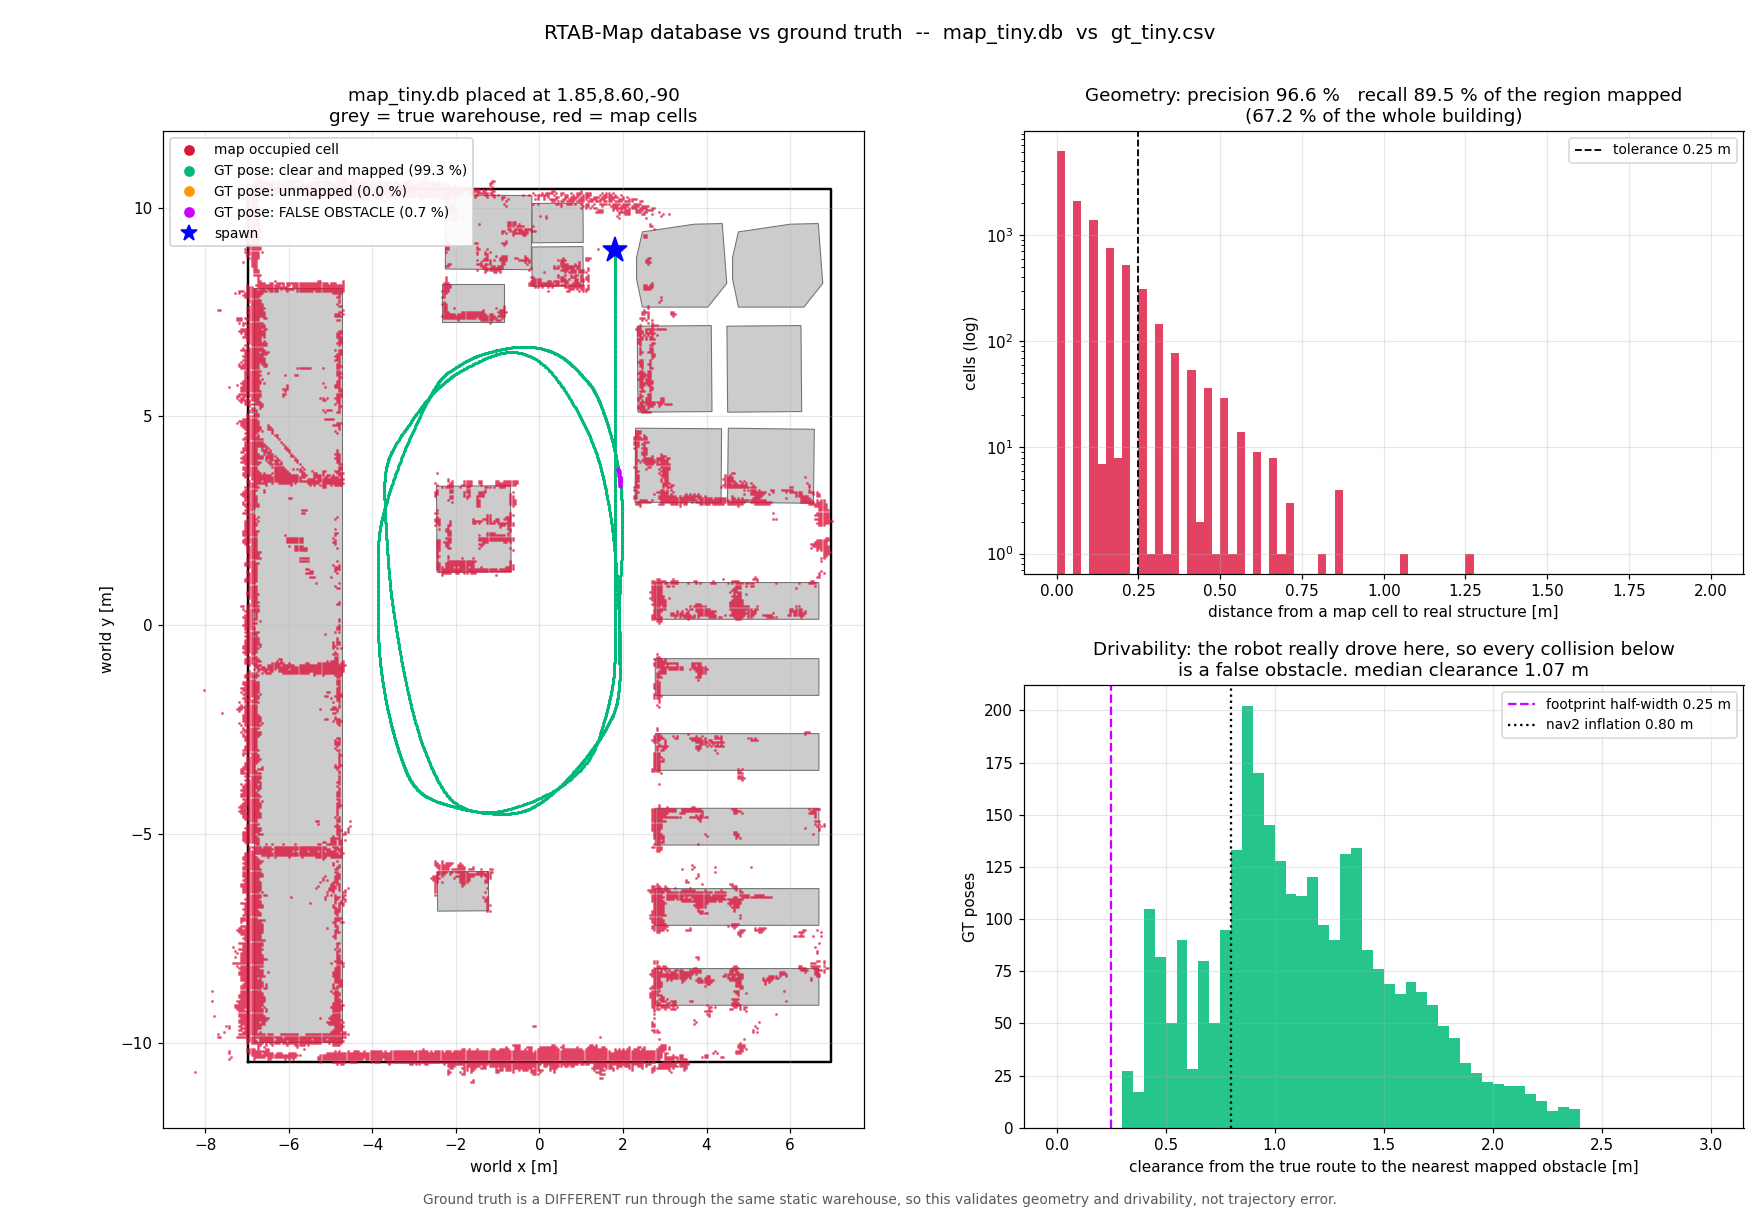
\includegraphics[width=\textwidth]{../../../output/compare/rtab_map_vs_gt.png}
  \caption[Dense-map evaluation of \repo{map/map_tiny.db}.]{Dense-map evaluation of \repo{map/map_tiny.db}. Left: occupied cells
  (red) over the world file's true collision geometry (grey), with the
  ground-truth route coloured by drivability and the spawn marked. Top right:
  distance from each occupied cell to real structure, with the
  \SI{0.25}{\metre} tolerance marked; the bulk falls well inside tolerance with a
  thin tail to about \SI{1.25}{\metre}. Bottom right: clearance from the true
  route to the nearest mapped obstacle, against the footprint half-width and the
  nav2 inflation radius. The ground truth was a different run through the same
  static warehouse, so this validates geometry and drivability, not trajectory
  error; that run is no longer available
  (\cref{sec:map-drivability}).}
  \label{fig:map-vs-gt}
\end{figure}

\begin{figure}[htbp]
  \centering
  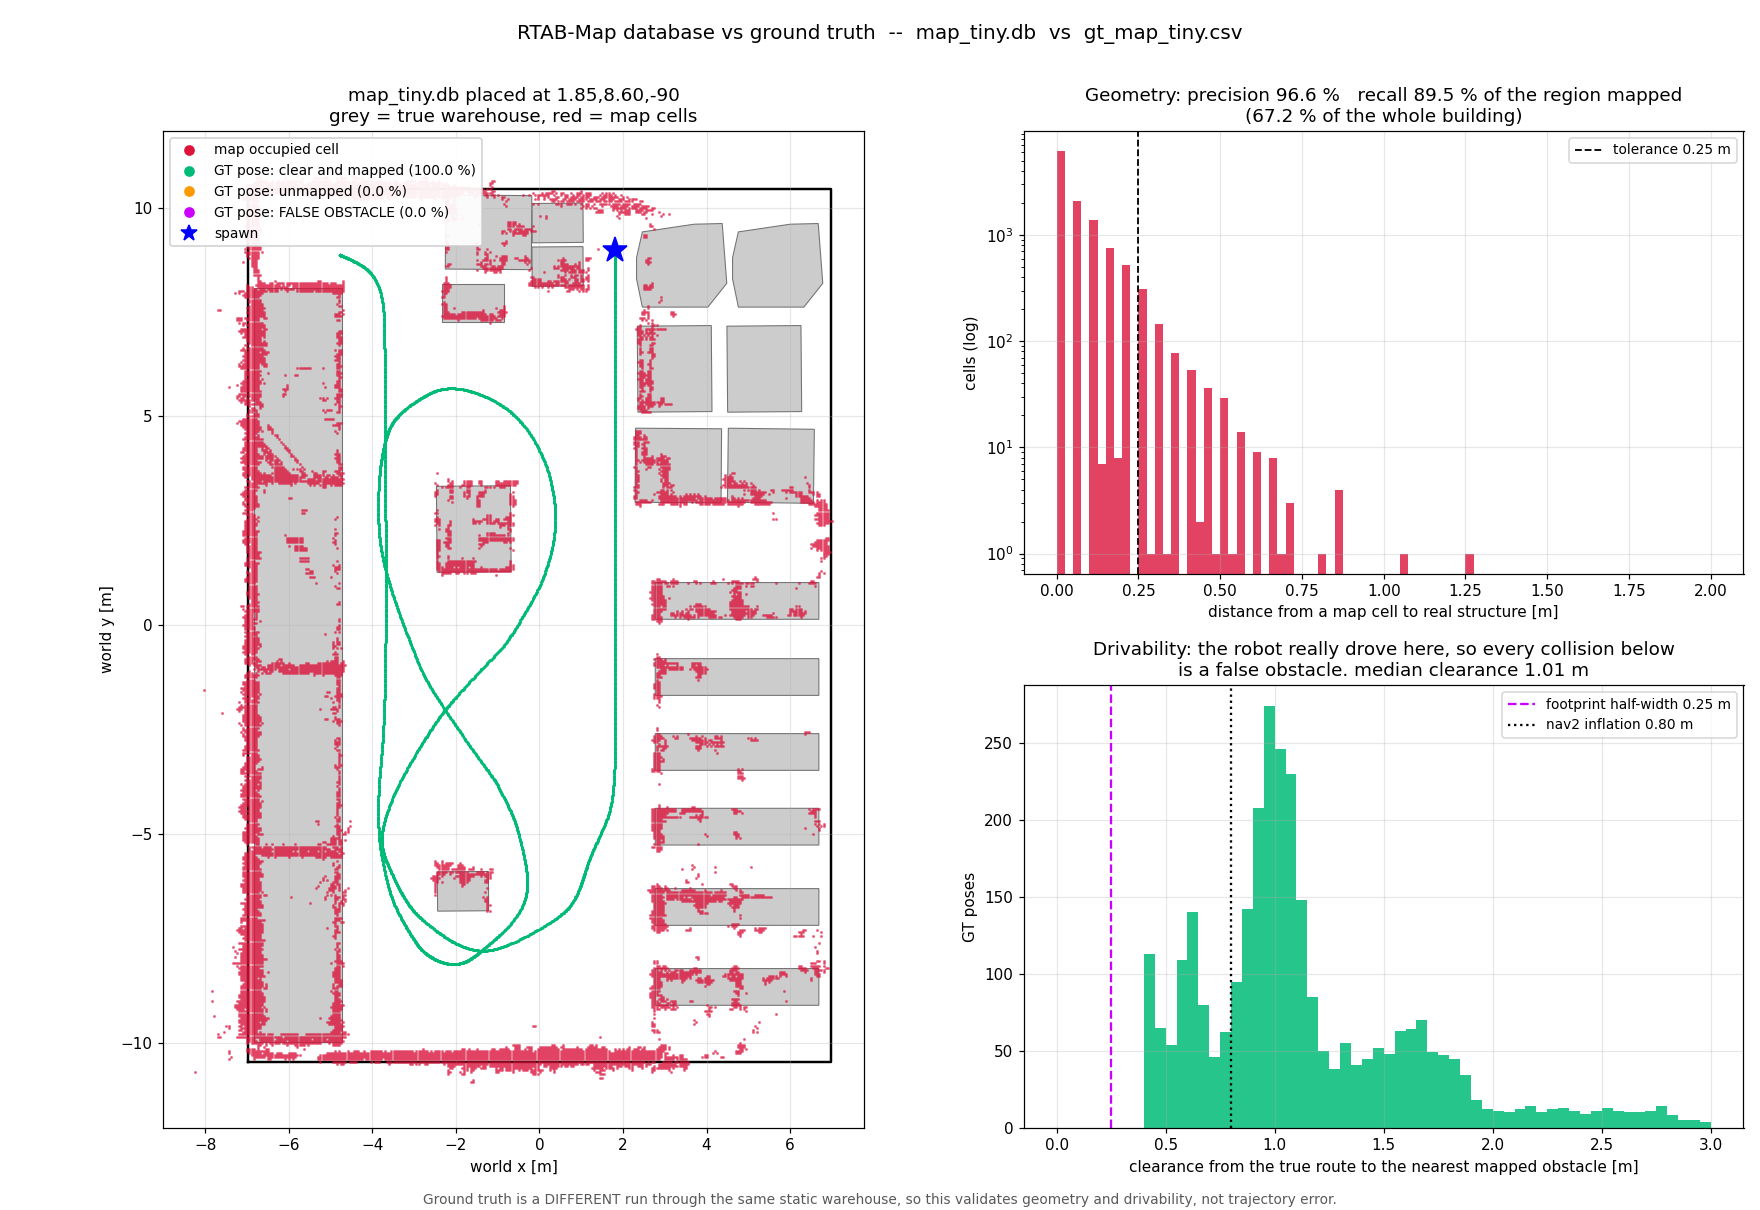
\includegraphics[width=\textwidth]{../../../output/compare/rtab_map_vs_gt_selfcheck.png}
  \caption[The same database scored against the run that built it, \repo{dataset/dataset_map_tiny}.]{The same database scored against the run that built it,
  \repo{dataset/dataset_map_tiny}. The route is a figure-eight rather than the
  oval of \cref{fig:map-vs-gt}, and no pose on it collides with the map: the
  false-obstacle rate falls from \SI{0.7}{\percent} to \SI{0.0}{\percent}. The
  geometry panels are identical to \cref{fig:map-vs-gt} because geometry does not
  depend on the route. The footer claiming a different run is emitted
  unconditionally by the evaluator and is incorrect for this figure.}
  \label{fig:map-vs-gt-selfcheck}
\end{figure}

\subsubsection{Interpretation and limitations}

Within its stated scope the tiny map is geometrically faithful and navigable:
\SI{96.6}{\percent} of what it marks as occupied is real, it recovers
\SI{89.5}{\percent} of the surfaces it actually observed, and it contains no blind
cells and only \SI{0.7}{\percent} proven false obstacles along a route the robot
really drove. The geometry half of that is independent evidence and is the
strongest map result the project currently holds; the drivability half is a
self-consistency check and is weaker than it looks. Both are a direct improvement
on earlier assessments that judged the same database unnavigable --- those were measured with the grid mis-seated, so the comparison
was against the wrong cells. That correction is a methodological finding in its
own right and is why \cref{sec:map-quality} reports placement before any metric.

Four limitations bound what these numbers support.

\begin{itemize}
  \item \textbf{The drivability reference cannot be re-read.} The run that
    provided it is lost, and the only surviving recording of this warehouse is the
    one that built the map, which would answer a weaker question. Re-establishing
    this result needs a fresh independent recording --- a second run, not a second
    map.
  \item \textbf{The route is easy.} It is one large loop down the wide central
    aisle and never squeezes into a side aisle. The \SI{0.7}{\percent} false-obstacle
    figure is therefore a floor, not a worst case. A route through the narrow
    aisles is the test that would actually stress this map, and it has not been
    run.
  \item \textbf{Clearance couples to planner cost.} The 5th-percentile clearance
    of \SI{0.45}{\metre} sits below nav2's \SI{0.80}{\metre} inflation radius, and
    a visible share of the true route lies inside it. Nothing is blocked, but a
    planner would charge a high cost for driving where the robot demonstrably
    drove. That coupling should be examined before any planned path is trusted.
  \item \textbf{$n=1$, and the scope is one world.} A single database on the tiny
    warehouse supports no uncertainty estimate and no claim about the large
    warehouse, where longer routes and narrower bays change both the drift
    exposure and the clearance margin.
  \item \textbf{Residual distortion is not a placement problem.} Walls appear
    doubled and thickened and shelf rows bowed in the overlay. No rigid transform
    removes that; it is internal map distortion and is the property that would
    limit navigation, independently of how well the grid is seated.
\end{itemize}

\begin{queried}[Queried: reproducibility of the drivability half]
The geometry result is fully reproducible: both \repo{map/map_tiny.db} and the
world file are present. The drivability result is not. Its reference run,
\repo{dataset_static_tiny_repeat}, is absent from \repo{dataset/} and from the
removable drive, and the only surviving recording of this warehouse is the one
that built the map, which would answer a weaker question
(\cref{sec:map-drivability}). The database additionally stores an empty parameter
set, so the configuration that produced it is not recoverable from the file, and
the RTAB-Map engineering record's claim that the node stamps match no dataset is
contradicted by the pose agreement reported above. The drivability figures should
therefore be read as a dated measurement rather than a standing result, and should
not be carried into the major report until an independent route has been recorded
and retained.
\end{queried}

\subsubsection{Planned extension to the large warehouse}

The same evaluation is \status{planned} for the large warehouse and is not
started: no large-map database exists at the cutoff. Three things must be settled
before those numbers would mean anything. The world-to-map placement must be
measured for the new database rather than assumed, since the tiny-map constant
$(1.850, 8.600, \SI{-89.90}{\degree})$ is specific to that database and world. A
ground-truth route must be recorded from a run \emph{other} than the one that
builds the map, which the tiny-map case did not do and which is what would turn
drivability into independent evidence. Finally, the route should deliberately
include narrow bays, so that the false-obstacle rate is exercised rather than
merely reported. Until then,
no map-quality claim extends beyond the tiny warehouse.


\subsubsection{Large-warehouse attempt}
\label{sec:map-large}

The progress update of 23 September 2026 reports that the large-warehouse map
attempt \status{failed}: the front end lost tracking in the repetitive bay
structure of the large world, the estimated pose diverged from the ground-truth
route within a few time steps of the loss, and the resulting map was not
scorable. The failure was attributed there to the front end under repeated
structure, not to the mapping back end.
\flag{No database, run directory or figure for this attempt is registered in
the repository at
the cutoff, so the result is reported on the strength of the progress record
and cannot yet be audited. The attempt must be repeated with its artifacts
retained before it is carried into any conclusion.}

\paragraph{Summary.} The mapping pipeline is geometrically sound where tracking
is sound: on the tiny map, occupied-cell precision is \SI{96.6}{\percent} and
observed-surface recall \SI{89.5}{\percent}, and the whole-building recall of
\SI{67.2}{\percent} is route coverage, not mapping failure. The drivability
half is a dated measurement whose independent route is lost. On the large map
the pipeline fails through repetitive structure, before the back end is
exercised.

\paragraph{Future plan.} Study methods robust to repeated features
(place-recognition gating, geometric verification of loop candidates); enable
ORB-SLAM3's Atlas so that a tracking loss opens a new sub-map instead of
corrupting the existing one, merging sub-maps afterwards; and record an
independent route on both maps and score drivability against it.

\subsection{Real robot}
\label{sec:exp4-real}

\slotstatus{planned}{No RTAB-Map database has been built from real imagery, and
no reference geometry of the site exists to score one against.}

\textbf{Reason.} The geometry metric of \cref{sec:map-eval-method} scores
occupied cells against known collision geometry; the real site has no such
model yet, and the placement step needs it. The drivability metric needs the
motion-capture route. Neither input exists at the cutoff.

\textbf{Next action.} Survey the mock warehouse (walls, stacks, walkway) into a
reference occupancy grid at the same \SI{0.05}{\metre} resolution, build a
database from a real mapping run, and then score it with the unchanged
evaluator, using a motion-capture route from a second run for drivability.

% =====================================================================
\section{Cross-Experiment Discussion, Simulation-to-Real Comparison and
Limitations}
\label{sec:results-discussion}

\subsection{Simulation against the real robot}

No simulation-to-real comparison can be drawn at the cutoff, because no
real-robot slot holds a valid result. What the simulation slots establish for
the real campaign is the order in which its risks should be retired: the noise
model matters more than the estimator architecture (\cref{sec:proprio-tuning}),
so the real IMU must be characterised before any pipeline is tuned; the
detector's miss rate bounds any filtering benefit (\cref{sec:yolo-performance}),
so real-image recall must be measured before the filter is judged; and the
front end, not the back end, is where the large-map failure sits
(\cref{sec:map-large}), so tracking robustness under repeated bay structure is
the first mapping risk on the real site.

% Verbatim from minor_report/chapters/chapter_4_results.tex lines 1730-1993 (retired report),
% headings demoted by 0 level(s). Do not edit here; edit the source of the numbers.

\subsection{Where each pipeline is weak, block by block}
\label{sec:block-performance}

\Cref{fig:blockperf-static,fig:blockperf-dynamic} put every instrumented stage of
the three pipelines on one page and colour it by a stated criterion.
\Cref{tab:blockperf-static-orb} through \cref{tab:blockperf-dynamic-vins} give the evidence behind every
colour: the metric, its value, the criterion it was tested against, and which of
three rules produced the verdict. Both the figures' fills and the tables are
generated by \repo{script/block_performance.py} from the run artifacts; no colour
in either figure was chosen by hand.

The three rules are deliberately distinguished, because they answer different
questions and only one of them is about accuracy:

\begin{description}[leftmargin=2.2em,style=nextline]
  \item[ablation] The block was removed, disabled or swapped and the run repeated.
    The value is the ratio of aligned ATE without it to aligned ATE with it. This
    is the only rule that speaks to trajectory error.
  \item[latency] The block's median time as a share of its stage, or a stage
    against the \SI{66.0}{\milli\second} inter-frame budget implied by
    \SI{30.3}{\hertz} imagery at $0.5\times$ replay. Describes cost, not accuracy.
  \item[outcome] A counter the block emits, against a stated threshold---accepted
    loop candidates, usable solver solutions, filter consistency.
\end{description}

\paragraph{Where the criteria come from.}
Every verdict is a comparison against a threshold, and those thresholds do not all
have the same standing. The tables label each one, and the distinction matters
more than the values:

\begin{description}[leftmargin=2.4em,style=nextline]
  \item[\textit{derived}] Follows from something outside this report. There are
    two. The \SI{66.0}{\milli\second} frame budget is arithmetic on the recorded
    conditions, $1000/(30.3\,\mathrm{Hz}\times0.5$ replay$)$: a per-frame stage
    slower than this cannot keep up, and no judgement is involved. The consistency
    target $\mathrm{ANEES}=3.0$ is the standard result that a correctly scaled
    covariance makes the normalised error squared average the degrees of freedom,
    which for a pose error is three.
  \item[\textit{convention}] A round number adopted here so the rule is stated
    rather than left implicit. Nothing external fixes \SI{40}{\percent} of a stage
    rather than \SI{35}{\percent}, $2.0\times$ for a load-bearing block rather than
    $1.5\times$, \SI{10}{\percent} of loop candidates accepted, or
    \SI{99}{\percent} of solver calls returning a usable solution. These are
    contestable, which is why the measured value sits beside the threshold in
    every row: a reader who prefers a different line can redraw it without
    re-running anything.
\end{description}

\begin{queried}[Withdrawn criterion]
An earlier revision of these tables graded VINS-Fusion's solver quality against
``median final cost $>5000$''. That threshold was chosen after observing 1176 in
static scenes and 14110 in dynamic ones, so it separated two numbers already in
hand and the \flag{``poor'' verdict it produced was guaranteed by the choice
rather than tested by it}. Raw Ceres cost also has no absolute scale, depending on
residual count and weighting, so no fixed threshold on it is meaningful in
principle. It is replaced by the solver's own \repo{solver_solution_usable} flag,
which is binary and emitted by the solver rather than invented here:
\SI{99.64}{\percent} of solves in static scenes and \SI{99.55}{\percent} in
dynamic ones return a usable solution, and the block is now graded \perfmark{good}
in both. The non-convergence rate---\SI{22.9}{\percent} of solves in static scenes
and \SI{45.3}{\percent} in dynamic ones reaching the iteration or
\SI{80}{\milli\second} cap---is reported in the note column and deliberately not
graded, because any threshold on it would repeat the same error.
\end{queried}

\begin{queried}[Reading the colours]
A red block is \emph{not} a claim that it caused the trajectory error, unless its
rule is \texttt{ablation}. Only four blocks in the entire project have an
ablation behind them: the EKF's wheel correction, its IMU prediction, its
yaw-rate model, and ORB-SLAM3's loop closing. Every other red marks a block that
is expensive or that emits a poor counter, which is a different and weaker
statement. Yellow means no claim at all---not instrumented, not exercised in these
runs, or not implemented in this fork.
\end{queried}

\begin{figure}[p]
  \centering
  %% Generated by script/block_performance.py -- do not edit.
\expandafter\def\csname blockcolour@static@orbextract\endcsname{perfpoor}
\expandafter\def\csname blockcolour@static@orbimupre\endcsname{perfgood}
\expandafter\def\csname blockcolour@static@orbposepred\endcsname{perfgood}
\expandafter\def\csname blockcolour@static@orbtracklocal\endcsname{perfgood}
\expandafter\def\csname blockcolour@static@orbkfdec\endcsname{perfgood}
\expandafter\def\csname blockcolour@static@orbkfins\endcsname{perfgood}
\expandafter\def\csname blockcolour@static@orbmpcull\endcsname{perfgood}
\expandafter\def\csname blockcolour@static@orbnewpoints\endcsname{perfgood}
\expandafter\def\csname blockcolour@static@orblba\endcsname{perfpoor}
\expandafter\def\csname blockcolour@static@orbkfcull\endcsname{perfgood}
\expandafter\def\csname blockcolour@static@orbtrackingtotal\endcsname{perfgood}
\expandafter\def\csname blockcolour@static@orbimuinit\endcsname{perfgood}
\expandafter\def\csname blockcolour@static@orbimuref\endcsname{perfgood}
\expandafter\def\csname blockcolour@static@orbplacerec\endcsname{perfpoor}
\expandafter\def\csname blockcolour@static@orbloopfusion\endcsname{perfpoor}
\expandafter\def\csname blockcolour@static@orbfullba\endcsname{perfnone}
\expandafter\def\csname blockcolour@static@orbyolo\endcsname{perfnone}
\expandafter\def\csname blockcolour@static@vinstrack\endcsname{perfgood}
\expandafter\def\csname blockcolour@static@vinsqueue\endcsname{perfpoor}
\expandafter\def\csname blockcolour@static@vinsimuprop\endcsname{perfgood}
\expandafter\def\csname blockcolour@static@vinstri\endcsname{perfgood}
\expandafter\def\csname blockcolour@static@vinsconstruct\endcsname{perfgood}
\expandafter\def\csname blockcolour@static@vinssolve\endcsname{perfpoor}
\expandafter\def\csname blockcolour@static@vinsmarg\endcsname{perfgood}
\expandafter\def\csname blockcolour@static@vinsoutlier\endcsname{perfgood}
\expandafter\def\csname blockcolour@static@vinsslide\endcsname{perfgood}
\expandafter\def\csname blockcolour@static@vinsbackendtotal\endcsname{perfpoor}
\expandafter\def\csname blockcolour@static@vinssolverq\endcsname{perfgood}
\expandafter\def\csname blockcolour@static@vinsloop\endcsname{perfnone}
\expandafter\def\csname blockcolour@static@vinsrtab\endcsname{perfnone}
\expandafter\def\csname blockcolour@static@vinsyolo\endcsname{perfnone}
\expandafter\def\csname blockcolour@static@ekfwheelupd\endcsname{perfgood}
\expandafter\def\csname blockcolour@static@ekfbiasobs\endcsname{perfgood}
\expandafter\def\csname blockcolour@static@ekfimupred\endcsname{perfgood}
\expandafter\def\csname blockcolour@static@ekfyaw\endcsname{perfpoor}
\expandafter\def\csname blockcolour@static@ekfanchor\endcsname{perfnone}
\expandafter\def\csname blockcolour@static@ekfcov\endcsname{perfpoor}
%
  \resizebox{\textwidth}{!}{\pipelinefig{static}}
  \caption[Per-block performance in the \textbf{static} condition, over the five \repo{allsensor} datasets.]{Per-block performance in the \textbf{static} condition, over the five
  \repo{allsensor} datasets. The EKF baseline appears here and not in
  \cref{fig:blockperf-dynamic} because no dynamic dataset carries wheel encoders.
  Evidence for every colour is in \cref{tab:blockperf-static-orb,tab:blockperf-static-vins,tab:blockperf-static-ekf}, one table per algorithm.}
  \label{fig:blockperf-static}
\end{figure}
\clearpage

\begin{table}[p]
\centering
\caption[Per-block evidence for \textbf{ORB-SLAM3} in the static condition, \cref{fig:blockperf-static}.]{Per-block evidence for \textbf{ORB-SLAM3} in the static condition, \cref{fig:blockperf-static}. Five \repo{allsensor} datasets, median across runs, loop closing enabled (\repo{logging_20260916_01}).}
\label{tab:blockperf-static-orb}
\scriptsize
\setlength{\tabcolsep}{3pt}
%% Generated by script/block_performance.py -- do not edit.
\begin{tabularx}{\textwidth}{>{\raggedright\arraybackslash}p{0.155\textwidth}l>{\raggedright\arraybackslash}X r>{\raggedright\arraybackslash}p{0.20\textwidth}l}
\toprule
Block & Rule & Metric & Value & Criterion / note & Verdict \\
\midrule
\multicolumn{6}{l}{\textbf{Tracking}} \\
\addlinespace[2pt]
\quad Extract ORB (+preproc, stereo) & latency & median image\_preprocessing\_feature\_stereo\_ms & \num{33.1} & \textit{convention:} $<$40\% of stage (61.4\% of stage) & \perfmark{poor} \\
\addlinespace[3.5pt]
\quad IMU preintegration & latency & median imu\_preintegration\_ms & \num{0.120} & \textit{convention:} $<$40\% of stage (0.2\% of stage) & \perfmark{good} \\
\addlinespace[3.5pt]
\quad Initial pose estimation & latency & median pose\_prediction\_ms & \num{0.087} & \textit{convention:} $<$40\% of stage (0.2\% of stage) & \perfmark{good} \\
\addlinespace[3.5pt]
\quad Track local map & latency & median local\_map\_tracking\_ms & \num{16.5} & \textit{convention:} $<$40\% of stage (30.7\% of stage) & \perfmark{good} \\
\addlinespace[3.5pt]
\quad New keyframe decision & latency & median keyframe\_decision\_ms & \num{0.169} & \textit{convention:} $<$40\% of stage (0.3\% of stage) & \perfmark{good} \\
\addlinespace[3.5pt]
\quad TRACKING total & latency & median tracking\_total\_ms & \num{53.8} & \textit{derived:} $<$\SI{66.0}{\milli\second} frame budget & \perfmark{good} \\
\addlinespace[3.5pt]
\quad Dynamic feature removal (YOLO) & none & -- & -- & -- (filter disabled in every run reported here) & \perfmark{none} \\
\addlinespace[3.5pt]
\addlinespace[5pt]
\multicolumn{6}{l}{\textbf{Local mapping}} \\
\addlinespace[2pt]
\quad KeyFrame insertion & latency & median keyframe\_insertion\_ms & \num{10.3} & \textit{convention:} $<$40\% of stage (3.3\% of stage) & \perfmark{good} \\
\addlinespace[3.5pt]
\quad Recent MapPoints culling & latency & median map\_point\_culling\_ms & \num{0.383} & \textit{convention:} $<$40\% of stage (0.1\% of stage) & \perfmark{good} \\
\addlinespace[3.5pt]
\quad New points creation & latency & median map\_point\_creation\_fusion\_ms & \num{41.5} & \textit{convention:} $<$40\% of stage (13.3\% of stage) & \perfmark{good} \\
\addlinespace[3.5pt]
\quad Local BA & latency & median local\_ba\_ms & \num{244.4} & \textit{convention:} $<$40\% of stage (78.1\% of stage) & \perfmark{poor} \\
\addlinespace[3.5pt]
\quad Local keyframes culling & latency & median keyframe\_culling\_ms & \num{10.9} & \textit{convention:} $<$40\% of stage (3.5\% of stage) & \perfmark{good} \\
\addlinespace[3.5pt]
\quad IMU initialization & latency & median imu\_initialization\_ms & \num{0.002} & \textit{convention:} $<$40\% of stage (negligible) & \perfmark{good} \\
\addlinespace[3.5pt]
\quad IMU scale refinement & latency & median inertial\_refinement\_ms & \num{0.001} & \textit{convention:} $<$40\% of stage (negligible) & \perfmark{good} \\
\addlinespace[3.5pt]
\addlinespace[5pt]
\multicolumn{6}{l}{\textbf{Loop closing}} \\
\addlinespace[2pt]
\quad Place recognition & outcome & candidates accepted & 4 of 281 & \textit{convention:} $>$\SI{10}{\percent} of candidates accepted (2494 events) & \perfmark{poor} \\
\addlinespace[3.5pt]
\quad Loop fusion + essential graph & ablation & ATE(on)/ATE(off) & 1.37 & \textit{convention:} $<$1.0 (enabling it should help) (one run per configuration) & \perfmark{poor} \\
\addlinespace[3.5pt]
\quad Full BA & outcome & global BA executions & -- & -- (see \cref{tab:orb-loop}) & \perfmark{none} \\
\addlinespace[3.5pt]
\bottomrule
\end{tabularx}

\end{table}
\clearpage
\begin{table}[p]
\centering
\caption[Per-block evidence for \textbf{VINS-Fusion} in the static condition, \cref{fig:blockperf-static}.]{Per-block evidence for \textbf{VINS-Fusion} in the static condition, \cref{fig:blockperf-static}. Five \repo{allsensor} datasets, median across runs.}
\label{tab:blockperf-static-vins}
\scriptsize
\setlength{\tabcolsep}{3pt}
%% Generated by script/block_performance.py -- do not edit.
\begin{tabularx}{\textwidth}{>{\raggedright\arraybackslash}p{0.155\textwidth}l>{\raggedright\arraybackslash}X r>{\raggedright\arraybackslash}p{0.20\textwidth}l}
\toprule
Block & Rule & Metric & Value & Criterion / note & Verdict \\
\midrule
\multicolumn{6}{l}{\textbf{Front end}} \\
\addlinespace[2pt]
\quad Feature tracking & latency & median feature\_tracking\_ms & \num{55.2} & $<$\SI{66.0}{\milli\second} frame budget & \perfmark{good} \\
\addlinespace[3.5pt]
\quad Feature queue & latency & median feature\_queue\_wait\_ms & \num{403.7} & $<$\SI{66.0}{\milli\second} frame budget (backlog 4.0 frames) & \perfmark{poor} \\
\addlinespace[3.5pt]
\quad Persistent-feature removal (YOLO) & none & -- & -- & -- (filter disabled in every run reported here) & \perfmark{none} \\
\addlinespace[3.5pt]
\addlinespace[5pt]
\multicolumn{6}{l}{\textbf{Back end}} \\
\addlinespace[2pt]
\quad IMU propagation & latency & median imu\_propagation\_ms & \num{0.272} & \textit{convention:} $<$40\% of stage (0.4\% of stage) & \perfmark{good} \\
\addlinespace[3.5pt]
\quad Triangulation & latency & median triangulation\_ms & \num{0.063} & \textit{convention:} $<$40\% of stage (0.1\% of stage) & \perfmark{good} \\
\addlinespace[3.5pt]
\quad Problem construction & latency & median problem\_construction\_ms & \num{3.2} & \textit{convention:} $<$40\% of stage (4.7\% of stage) & \perfmark{good} \\
\addlinespace[3.5pt]
\quad Ceres solve & latency & median solver\_ms & \num{48.3} & \textit{convention:} $<$40\% of stage (71.9\% of stage) & \perfmark{poor} \\
\addlinespace[3.5pt]
\quad Marginalization & latency & median marginalization\_ms & \num{4.1} & \textit{convention:} $<$40\% of stage (6.1\% of stage) & \perfmark{good} \\
\addlinespace[3.5pt]
\quad Outlier rejection & latency & median outlier\_rejection\_ms & \num{0.155} & \textit{convention:} $<$40\% of stage (0.2\% of stage) & \perfmark{good} \\
\addlinespace[3.5pt]
\quad Slide window & latency & median slide\_window\_ms & \num{0.212} & \textit{convention:} $<$40\% of stage (0.3\% of stage) & \perfmark{good} \\
\addlinespace[3.5pt]
\quad BACK END total & latency & median backend\_total\_ms & \num{67.2} & $<$\SI{66.0}{\milli\second} frame budget & \perfmark{poor} \\
\addlinespace[3.5pt]
\quad Solver convergence & outcome & solves returning a usable solution & 99.64\% & \textit{convention:} $\geq$\SI{99}{\percent} usable (\SI{22.8}{\percent} hit the iteration or \SI{80}{\milli\second} cap without converging; reported, not graded) & \perfmark{good} \\
\addlinespace[3.5pt]
\addlinespace[5pt]
\multicolumn{6}{l}{\textbf{Loop closing}} \\
\addlinespace[2pt]
\quad Loop fusion & none & -- & -- & -- (not implemented in this fork) & \perfmark{none} \\
\addlinespace[3.5pt]
\quad RTAB-Map correction & none & -- & -- & -- (separate process; correction never injected) & \perfmark{none} \\
\addlinespace[3.5pt]
\bottomrule
\end{tabularx}

\end{table}
\clearpage
\begin{table}[p]
\centering
\caption[Per-block evidence for the \textbf{EKF wheel\,+\,IMU} baseline, \cref{fig:blockperf-static}.]{Per-block evidence for the \textbf{EKF wheel\,+\,IMU} baseline, \cref{fig:blockperf-static}. Every row but the last two is an ablation: the block was removed or swapped and all five datasets re-run, so these are the only verdicts in this section that speak to trajectory error.}
\label{tab:blockperf-static-ekf}
\scriptsize
\setlength{\tabcolsep}{3pt}
%% Generated by script/block_performance.py -- do not edit.
\begin{tabularx}{\textwidth}{>{\raggedright\arraybackslash}p{0.155\textwidth}l>{\raggedright\arraybackslash}X r>{\raggedright\arraybackslash}p{0.20\textwidth}l}
\toprule
Block & Rule & Metric & Value & Criterion / note & Verdict \\
\midrule
\multicolumn{6}{l}{\textbf{EKF}} \\
\addlinespace[2pt]
\quad Wheel speed correction & ablation & ATE without the wheel update / with & 54.08 & \textit{convention:} $\geq$2.0$\times$ (block is load-bearing) (median over 5 bags; joint with the other row -- one flag removes both) & \perfmark{good} \\
\addlinespace[3.5pt]
\quad Gyro-bias observation & ablation & ATE without the wheel update / with & 54.08 & \textit{convention:} $\geq$2.0$\times$ (block is load-bearing) (median over 5 bags; joint with the other row -- one flag removes both) & \perfmark{good} \\
\addlinespace[3.5pt]
\quad IMU prediction & ablation & ATE of wheel-only / EKF & 6.56 & \textit{convention:} $\geq$2.0$\times$ (block is load-bearing) (median over 5 bags) & \perfmark{good} \\
\addlinespace[3.5pt]
\quad Yaw-rate model (bicycle) & ablation & ATE with differential / with bicycle & 1.02 & \textit{convention:} $\geq$2.0$\times$ (block is load-bearing) (median over 5 bags) & \perfmark{poor} \\
\addlinespace[3.5pt]
\quad Initial pose anchor & none & -- & -- & -- (ground-truth pose; not a performance block) & \perfmark{none} \\
\addlinespace[3.5pt]
\quad Covariance propagation & outcome & ANEES (3 DOF) & -- & \textit{derived:} 3.0 for a consistent filter (64.7--123.2; see \cref{tab:proprio-covariance}) & \perfmark{poor} \\
\addlinespace[3.5pt]
\bottomrule
\end{tabularx}

\end{table}
\clearpage
\begin{figure}[p]
  \centering
  %% Generated by script/block_performance.py -- do not edit.
\expandafter\def\csname blockcolour@dynamic@orbextract\endcsname{perfpoor}
\expandafter\def\csname blockcolour@dynamic@orbimupre\endcsname{perfgood}
\expandafter\def\csname blockcolour@dynamic@orbposepred\endcsname{perfgood}
\expandafter\def\csname blockcolour@dynamic@orbtracklocal\endcsname{perfgood}
\expandafter\def\csname blockcolour@dynamic@orbkfdec\endcsname{perfgood}
\expandafter\def\csname blockcolour@dynamic@orbkfins\endcsname{perfgood}
\expandafter\def\csname blockcolour@dynamic@orbmpcull\endcsname{perfgood}
\expandafter\def\csname blockcolour@dynamic@orbnewpoints\endcsname{perfgood}
\expandafter\def\csname blockcolour@dynamic@orblba\endcsname{perfpoor}
\expandafter\def\csname blockcolour@dynamic@orbkfcull\endcsname{perfgood}
\expandafter\def\csname blockcolour@dynamic@orbtrackingtotal\endcsname{perfgood}
\expandafter\def\csname blockcolour@dynamic@orbimuinit\endcsname{perfnone}
\expandafter\def\csname blockcolour@dynamic@orbimuref\endcsname{perfnone}
\expandafter\def\csname blockcolour@dynamic@orbplacerec\endcsname{perfpoor}
\expandafter\def\csname blockcolour@dynamic@orbloopfusion\endcsname{perfnone}
\expandafter\def\csname blockcolour@dynamic@orbfullba\endcsname{perfnone}
\expandafter\def\csname blockcolour@dynamic@orbyolo\endcsname{perfnone}
\expandafter\def\csname blockcolour@dynamic@vinstrack\endcsname{perfgood}
\expandafter\def\csname blockcolour@dynamic@vinsqueue\endcsname{perfpoor}
\expandafter\def\csname blockcolour@dynamic@vinsimuprop\endcsname{perfgood}
\expandafter\def\csname blockcolour@dynamic@vinstri\endcsname{perfgood}
\expandafter\def\csname blockcolour@dynamic@vinsconstruct\endcsname{perfgood}
\expandafter\def\csname blockcolour@dynamic@vinssolve\endcsname{perfpoor}
\expandafter\def\csname blockcolour@dynamic@vinsmarg\endcsname{perfgood}
\expandafter\def\csname blockcolour@dynamic@vinsoutlier\endcsname{perfgood}
\expandafter\def\csname blockcolour@dynamic@vinsslide\endcsname{perfgood}
\expandafter\def\csname blockcolour@dynamic@vinsbackendtotal\endcsname{perfgood}
\expandafter\def\csname blockcolour@dynamic@vinssolverq\endcsname{perfgood}
\expandafter\def\csname blockcolour@dynamic@vinsloop\endcsname{perfnone}
\expandafter\def\csname blockcolour@dynamic@vinsrtab\endcsname{perfnone}
\expandafter\def\csname blockcolour@dynamic@vinsyolo\endcsname{perfnone}
%
  \resizebox{\textwidth}{!}{\pipelinefig{dynamic}}
  \caption[Per-block performance in the \textbf{dynamic} condition, over the twelve relogged dynamic runs of each estimator.]{Per-block performance in the \textbf{dynamic} condition, over the
  twelve relogged dynamic runs of each estimator. Loop closing carries no
  ablation here because the relogged campaign has no loop-closure-disabled
  variant. Evidence in \cref{tab:blockperf-dynamic-orb,tab:blockperf-dynamic-vins},
  one table per algorithm.}
  \label{fig:blockperf-dynamic}
\end{figure}
\clearpage
\begin{table}[p]
\centering
\caption[Per-block evidence for \textbf{ORB-SLAM3} in the dynamic condition, \cref{fig:blockperf-dynamic}.]{Per-block evidence for \textbf{ORB-SLAM3} in the dynamic condition, \cref{fig:blockperf-dynamic}. Twelve relogged dynamic runs, median across runs.}
\label{tab:blockperf-dynamic-orb}
\scriptsize
\setlength{\tabcolsep}{3pt}
%% Generated by script/block_performance.py -- do not edit.
\begin{tabularx}{\textwidth}{>{\raggedright\arraybackslash}p{0.155\textwidth}l>{\raggedright\arraybackslash}X r>{\raggedright\arraybackslash}p{0.20\textwidth}l}
\toprule
Block & Rule & Metric & Value & Criterion / note & Verdict \\
\midrule
\multicolumn{6}{l}{\textbf{Tracking}} \\
\addlinespace[2pt]
\quad Extract ORB (+preproc, stereo) & latency & median image\_preprocessing\_feature\_stereo\_ms & \num{45.1} & \textit{convention:} $<$40\% of stage (73.8\% of stage) & \perfmark{poor} \\
\addlinespace[3.5pt]
\quad IMU preintegration & latency & median imu\_preintegration\_ms & \num{0.116} & \textit{convention:} $<$40\% of stage (0.2\% of stage) & \perfmark{good} \\
\addlinespace[3.5pt]
\quad Initial pose estimation & latency & median pose\_prediction\_ms & \num{0.055} & \textit{convention:} $<$40\% of stage (0.1\% of stage) & \perfmark{good} \\
\addlinespace[3.5pt]
\quad Track local map & latency & median local\_map\_tracking\_ms & \num{12.2} & \textit{convention:} $<$40\% of stage (19.9\% of stage) & \perfmark{good} \\
\addlinespace[3.5pt]
\quad New keyframe decision & latency & median keyframe\_decision\_ms & \num{0.179} & \textit{convention:} $<$40\% of stage (0.3\% of stage) & \perfmark{good} \\
\addlinespace[3.5pt]
\quad TRACKING total & latency & median tracking\_total\_ms & \num{61.2} & \textit{derived:} $<$\SI{66.0}{\milli\second} frame budget & \perfmark{good} \\
\addlinespace[3.5pt]
\quad Dynamic feature removal (YOLO) & none & -- & -- & -- (filter disabled in every run reported here) & \perfmark{none} \\
\addlinespace[3.5pt]
\addlinespace[5pt]
\multicolumn{6}{l}{\textbf{Local mapping}} \\
\addlinespace[2pt]
\quad KeyFrame insertion & latency & median keyframe\_insertion\_ms & \num{10.9} & \textit{convention:} $<$40\% of stage (5.7\% of stage) & \perfmark{good} \\
\addlinespace[3.5pt]
\quad Recent MapPoints culling & latency & median map\_point\_culling\_ms & \num{0.714} & \textit{convention:} $<$40\% of stage (0.4\% of stage) & \perfmark{good} \\
\addlinespace[3.5pt]
\quad New points creation & latency & median map\_point\_creation\_fusion\_ms & \num{50.0} & \textit{convention:} $<$40\% of stage (26.3\% of stage) & \perfmark{good} \\
\addlinespace[3.5pt]
\quad Local BA & latency & median local\_ba\_ms & \num{122.9} & \textit{convention:} $<$40\% of stage (64.6\% of stage) & \perfmark{poor} \\
\addlinespace[3.5pt]
\quad Local keyframes culling & latency & median keyframe\_culling\_ms & \num{4.0} & \textit{convention:} $<$40\% of stage (2.1\% of stage) & \perfmark{good} \\
\addlinespace[3.5pt]
\quad IMU initialization & latency & median imu\_initialization\_ms & -- & \textit{convention:} $<$40\% of stage (not logged) & \perfmark{none} \\
\addlinespace[3.5pt]
\quad IMU scale refinement & latency & median inertial\_refinement\_ms & -- & \textit{convention:} $<$40\% of stage (not logged) & \perfmark{none} \\
\addlinespace[3.5pt]
\addlinespace[5pt]
\multicolumn{6}{l}{\textbf{Loop closing}} \\
\addlinespace[2pt]
\quad Place recognition & outcome & candidates accepted & 0 of 2 & \textit{convention:} $>$\SI{10}{\percent} of candidates accepted (5726 events) & \perfmark{poor} \\
\addlinespace[3.5pt]
\quad Loop fusion + essential graph & ablation & ATE(on)/ATE(off) & -- & \textit{convention:} $<$1.0 (enabling it should help) (one run per configuration) & \perfmark{none} \\
\addlinespace[3.5pt]
\quad Full BA & outcome & global BA executions & -- & -- (see \cref{tab:orb-loop}) & \perfmark{none} \\
\addlinespace[3.5pt]
\bottomrule
\end{tabularx}

\end{table}
\clearpage
\begin{table}[p]
\centering
\caption[Per-block evidence for \textbf{VINS-Fusion} in the dynamic condition, \cref{fig:blockperf-dynamic}.]{Per-block evidence for \textbf{VINS-Fusion} in the dynamic condition, \cref{fig:blockperf-dynamic}. Twelve relogged dynamic runs, median across runs.}
\label{tab:blockperf-dynamic-vins}
\scriptsize
\setlength{\tabcolsep}{3pt}
%% Generated by script/block_performance.py -- do not edit.
\begin{tabularx}{\textwidth}{>{\raggedright\arraybackslash}p{0.155\textwidth}l>{\raggedright\arraybackslash}X r>{\raggedright\arraybackslash}p{0.20\textwidth}l}
\toprule
Block & Rule & Metric & Value & Criterion / note & Verdict \\
\midrule
\multicolumn{6}{l}{\textbf{Front end}} \\
\addlinespace[2pt]
\quad Feature tracking & latency & median feature\_tracking\_ms & \num{42.5} & $<$\SI{66.0}{\milli\second} frame budget & \perfmark{good} \\
\addlinespace[3.5pt]
\quad Feature queue & latency & median feature\_queue\_wait\_ms & \num{502.1} & $<$\SI{66.0}{\milli\second} frame budget (backlog 7.5 frames) & \perfmark{poor} \\
\addlinespace[3.5pt]
\quad Persistent-feature removal (YOLO) & none & -- & -- & -- (filter disabled in every run reported here) & \perfmark{none} \\
\addlinespace[3.5pt]
\addlinespace[5pt]
\multicolumn{6}{l}{\textbf{Back end}} \\
\addlinespace[2pt]
\quad IMU propagation & latency & median imu\_propagation\_ms & \num{0.204} & \textit{convention:} $<$40\% of stage (0.3\% of stage) & \perfmark{good} \\
\addlinespace[3.5pt]
\quad Triangulation & latency & median triangulation\_ms & \num{0.062} & \textit{convention:} $<$40\% of stage (0.1\% of stage) & \perfmark{good} \\
\addlinespace[3.5pt]
\quad Problem construction & latency & median problem\_construction\_ms & \num{1.1} & \textit{convention:} $<$40\% of stage (1.7\% of stage) & \perfmark{good} \\
\addlinespace[3.5pt]
\quad Ceres solve & latency & median solver\_ms & \num{57.2} & \textit{convention:} $<$40\% of stage (89.8\% of stage) & \perfmark{poor} \\
\addlinespace[3.5pt]
\quad Marginalization & latency & median marginalization\_ms & \num{2.4} & \textit{convention:} $<$40\% of stage (3.7\% of stage) & \perfmark{good} \\
\addlinespace[3.5pt]
\quad Outlier rejection & latency & median outlier\_rejection\_ms & \num{0.068} & \textit{convention:} $<$40\% of stage (0.1\% of stage) & \perfmark{good} \\
\addlinespace[3.5pt]
\quad Slide window & latency & median slide\_window\_ms & \num{0.167} & \textit{convention:} $<$40\% of stage (0.3\% of stage) & \perfmark{good} \\
\addlinespace[3.5pt]
\quad BACK END total & latency & median backend\_total\_ms & \num{63.7} & $<$\SI{66.0}{\milli\second} frame budget & \perfmark{good} \\
\addlinespace[3.5pt]
\quad Solver convergence & outcome & solves returning a usable solution & 99.55\% & \textit{convention:} $\geq$\SI{99}{\percent} usable (\SI{45.1}{\percent} hit the iteration or \SI{80}{\milli\second} cap without converging; reported, not graded) & \perfmark{good} \\
\addlinespace[3.5pt]
\addlinespace[5pt]
\multicolumn{6}{l}{\textbf{Loop closing}} \\
\addlinespace[2pt]
\quad Loop fusion & none & -- & -- & -- (not implemented in this fork) & \perfmark{none} \\
\addlinespace[3.5pt]
\quad RTAB-Map correction & none & -- & -- & -- (separate process; correction never injected) & \perfmark{none} \\
\addlinespace[3.5pt]
\bottomrule
\end{tabularx}

\end{table}
\clearpage


Four readings follow that the trajectory tables alone do not give.

\textbf{Both visual front ends are the dominant cost, and neither keeps up
cleanly.} ORB-SLAM3 spends \SI{33.1}{\milli\second} of a \SI{53.8}{\milli\second}
tracking budget on preprocessing, extraction and stereo matching in static scenes,
rising to \SI{45.1}{\milli\second} of \SI{61.2}{\milli\second} in dynamic ones.
VINS-Fusion's back end waits \SI{403.7}{\milli\second} per frame on its feature
queue in static scenes and \SI{502.1}{\milli\second} in dynamic ones, against a
\SI{66.0}{\milli\second} frame budget, with a backlog of four to seven frames.
\flag{These are the same deficit wearing different clothes}: neither estimator
processes frames as fast as they arrive, and the two differ in what they do about
it. ORB-SLAM3 subscribes best-effort at depth five and discards the overflow,
which is the frame shortfall of \cref{sec:results-validity}; VINS-Fusion
subscribes reliably at depth 100 and absorbs it as latency. The frame counters see
one and not the other.

\textbf{Local BA dominates ORB-SLAM3's local mapping} at \SI{244.4}{\milli\second}
of \SI{312.9}{\milli\second} in static scenes. It runs per keyframe rather than
per frame, so it does not compete directly with the frame budget, but it is where
that pipeline's compute goes.

\textbf{Loop closing is not earning its place in these scenes.} Across the five
\repo{allsensor} datasets, enabling it leaves the median aligned ATE
\num{1.37} times \emph{worse} than disabling it, and only 4 of 281 place-recognition
candidates were ever accepted (\cref{tab:orb-loop}). This is the project's one
ORB-SLAM3 ablation, and it is still one run per configuration, so it sits inside
an unmeasured run-to-run spread---the verdict is reported, not relied upon.

\textbf{The EKF's accuracy rests on one intervention.} Removing the wheel update
costs a factor of \num{54} in aligned ATE; removing the IMU prediction costs
\num{6.6}. The \num{54} covers the wheel speed correction and the gyroscope-bias
observation \emph{together}: both are measurement rows of the same update, one
flag removes both, and no flag removes only one, so
\cref{tab:blockperf-static-ekf} lists the figure against each row while marking it
as joint rather than presenting two independent results. Swapping the yaw-rate model from the bicycle formulation to the
rear-wheel differential, by contrast, changes nothing measurable---median
\num{1.0}, and on \repo{allsensor_004} the noisier estimator is the better one.
That is worth stating plainly, because the differential model is four times worse
as a \emph{rate} estimator (\cref{tab:proprio-noise}) and dominates standalone
wheel odometry's error. Inside the filter it barely matters, because the wheel
rate is used only to observe the gyroscope bias and is weighted by its own
measured $\sigma$. The design choice of \cref{sec:proprio-method} is vindicated by
its own ablation.

The campaign succeeds as an instrumentation milestone: repeated run-level data,
front-end and back-end timing, input retention, process resources, initialization,
tracking loss, keyframes, loop closures, map merges, and raw trajectories are now
available in auditable form. Ground-truth accuracy can now be measured, but the
campaign does not support the intended semantic-filter hypothesis or a clean
dynamic-scene estimator ranking. The limitations are:

\Cref{tab:limitations} lists them with the consequence each one carries.

\begin{table}[htbp]
\centering
\caption[Limitations of the results reported in this chapter, and what each one prevents.]{Limitations of the results reported in this chapter, and what each one
prevents. ``Scope'' identifies the experiment affected: R is the relogged
campaign, E the estimator comparison of \cref{sec:results-proprio}, and A both.}
\label{tab:limitations}
\small
\begin{tabularx}{\textwidth}{l>{\raggedright\arraybackslash}p{0.36\textwidth}>{\raggedright\arraybackslash}X}
\toprule
Scope & Limitation & Consequence \\
\midrule
A & RPE was missing & now implemented and reported (\cref{sec:rpe}); it
  withdrew this chapter's local-coherence reading \\
R & every dynamic trajectory fails the jump-plausibility criterion & no dynamic
  estimator ranking \\
R & the VINS semantic treatment was inactive in all repeats & no VINS filtering
  conclusion \\
R & 11 of 12 ORB treatment pairs fail the paired-input rule & no cross-treatment
  accuracy conclusion \\
R & YOLO truth is projected simulator geometry, not annotated visible extent, and
  the retained confidence threshold is fixed & no AP claim \\
R & class metrics are conditional on successful IoU localization & must not be
  read as end-to-end accuracy \\
R & two static ORB run summaries have incomplete schemas & retained as
  operational; counters unavailable \\
A & CPU and memory are per-estimator-process figures & not whole-system cost \\
A & one laptop and one replay rate throughout & no hardware or input-rate stress
  surface \\
E & \flag{replay rate $0.5\times$ for both visual estimators} & accuracy figures
  are not evidence of real-time capability \\
E & \flag{baselines are offline, visual estimators ran live} & timing-induced
  error is present on one side of the comparison only \\
E & \flag{only \repo{allsensor} bags carry wheel encoders} & the baseline exists
  for static featureless-floor scenes only; no dynamic condition \\
E & \flag{$n=5$ across four worlds, no condition repeated more than twice} & no
  mean, deviation or interval; between-bag differences are not effects \\
E & \flag{ORB-SLAM3 drops frames at a depth-5 best-effort subscriber; VINS buffers
  100 deep} & input delivery is not matched between the two; no timing comparison
  is admissible \\
E & \flag{ORB-SLAM3 run-to-run spread unmeasured, one run per configuration} &
  loop-closure differences cannot be attributed; repeats required \\
E & \flag{loop-closure state absent from \repo{run_metadata.csv}} & configurations
  distinguishable only by inspecting \repo{loop_closing.csv} \\
E & \flag{origin of the wheel yaw-rate offset untested} & the drift is predicted
  but not yet attributable or correctable (\cref{sec:h1-falsified}) \\
E & wheel-rate offset is absorbed by the EKF gyroscope-bias state & now
  quantified: EKF heading error rises tenfold where the wheel rate is poor
  (\cref{tab:ekf-coupling}) \\
E & \flag{accelerometer characterisation unstable across bags} & bias 0.019 to
  0.068, scale 1.020 to 1.067 for one simulated sensor \\
E & neither visual estimator writes a pose covariance & the consistency test
  cannot be applied to them \\
\bottomrule
\end{tabularx}
\end{table}

No root cause is assigned in this report. In particular, differences are not
attributed to calibration, timestamp handling, masks, replay scheduling, or a
specific estimator component without a controlled diagnostic experiment. The
immediate advisor decision is whether the next work period should first restore
active, input-matched filtering and plausible full trajectories, or
instead prioritize the planned integration of relocalization, global
optimization, and map merging. The latter remains future work and would provide
a unified localization/map input for navigation; path planning itself remains
outside scope.


% Chapter 5.  Conclusions are stated only as strongly as the filled slots of
% Chapter 4 allow; every claim points back to the slot that holds its evidence.
\chapter[CONCLUSION AND RECOMMENDATIONS]{Conclusion and Recommendations}
\label{chap:conclusion}

This project set out to replace infrastructure-based navigation with a
vision-based pipeline that stays accurate when the warehouse changes, and to
decide between two ways of building it. At the reporting cutoff the pipeline
exists in both forms, the four experiments that judge it are defined for both
domains, and the four simulation slots hold results. The four real-robot slots
do not. The conclusions below are therefore conclusions about the simulated
warehouse, and each is bounded by the validity limits recorded beside it in
\cref{chap:results}.

\section{Conclusions by Experiment}
\label{sec:conclusions}

\subsection{Experiment 1: is vision earning its place?}

On five static recordings, a five-state wheel-plus-gyroscope EKF whose noise
model is calibrated per recording localises to \SIrange{0.19}{0.49}{\metre}
aligned ATE, ahead of stereo visual-inertial SLAM running on a hand-set
configuration on four of five recordings (\cref{tab:proprio-accuracy}). That
ordering is not a property of the architectures: giving the filter the visual
systems' own inertial noise model degrades it on every recording and puts
VINS-Fusion ahead on all five (\cref{sec:proprio-tuning}). The defensible
conclusion is narrower than either reading: over this range the noise model is
worth more than the estimator, and the visual systems have never been tuned to
this platform. Two results survive the control. The proprioceptive sensors fail
in complementary ways, the IMU holding heading and losing position, the wheels
the reverse, and the EKF is better than either in both quantities because it
observes the gyroscope bias rather than the heading
(\cref{sec:h1-falsified}). And every dead-reckoning covariance is overconfident
by about two orders of magnitude (\cref{tab:proprio-covariance}). Against the
project's target of \SI{0.05}{\metre} ATE, no estimator qualifies; against the
\SI{1.5}{\metre} RPE target at \SI{1}{\second}, all of them do in static
scenes. The comparison is confined to static, encoder-equipped recordings and
to a floor on which the wheels effectively cannot slip.

\subsection{Experiment 2: how good is the detector?}

The three-class detector is reliable at naming and unreliable at finding:
pooled precision 0.684, moving-object recall 0.591, conditional class F1 0.995
over 9\,860 frames (\cref{tab:yolo-performance,tab:yolo-classification}). It
misses about \SI{41}{\percent} of the moving objects that are scored, and
\SI{62}{\percent} if every occluded or tiny object is counted; that miss rate is
the ceiling on any filtering benefit downstream. The ground truth is projected
simulator geometry rather than annotation, which makes the boxes tighter and the
scored subset easier than a human-labelled set, and no average precision is
reported because a single confidence threshold was retained.

\subsection{Experiment 3: does filtering help?}

The question the project is named for has no valid answer yet. Sixty-six runs
exist, fully instrumented, but the VINS-Fusion filter never activated, eleven
of twelve ORB-SLAM3 treatment pairs received different input, and the scripted
dynamic worlds were found to be an invalid testbed, so every dynamic-scene
trajectory is withheld as a finding (\cref{sec:trajectory-results}). This is
untested, not tested and failed. The static runs do establish two things: the
two front ends reach medians of \SI{0.370}{\metre} and \SI{0.454}{\metre}
aligned ATE, and ORB-SLAM3's eleven-fold rotational penalty is produced by one
or two discrete events near inertial initialisation, not by its steady-state
tracking (\cref{sec:rpe}). Neither front end keeps up with the frame rate at the
replay rate used, and they hide that deficit differently, one by dropping
frames and one by queueing them (\cref{sec:block-performance}).

\subsection{Experiment 4: is the map usable?}

Where tracking is sound, the mapping pipeline is: the tiny-warehouse map is
\SI{96.6}{\percent} precise in what it marks occupied, recovers
\SI{89.5}{\percent} of the surfaces it observed, and contains no blind cells and
\SI{0.7}{\percent} proven false obstacles along an independently driven route
(\cref{tab:map-geometry,tab:map-drivability}). The whole-building recall of
\SI{67.2}{\percent} is route coverage, not mapping failure. The drivability half
of that result is dated, because its independent route is lost. On the large
warehouse the attempt failed through tracking loss in repetitive structure,
before the back end was exercised, and its artifacts were not retained.

\section{Limitations and Threats to Validity}
\label{sec:limitations}

The limitations of \cref{tab:limitations} carry over without softening. The
ones that bound the conclusions above most tightly are these. Every result is
from one laptop at one replay rate, so nothing here is evidence of real-time
capability on the NRU-51V. The proprioceptive baseline exists only for static,
encoder-equipped, near-slip-free recordings, with $n=5$ across four worlds and
no condition repeated more than twice. ORB-SLAM3's run-to-run spread is
unmeasured and its loop-closure configuration is absent from the run manifest,
so its loop-closure results cannot be attributed. The detector is scored against
projected geometry with exemptions the training convention lacks. The dynamic
worlds move props kinematically and so do not pose the problem the project
poses. And no real-robot slot is filled: the rig's calibration has a
placeholder translation and a reused intrinsic set, and no recording carries
motion-capture truth, wheel odometry or varied illumination.

\section{Recommendations and Next Steps}
\label{sec:recommendations}

\textbf{Fill the four real-robot slots, in the order the simulation results
suggest.} First calibrate the real camera--IMU pair and record the
motion-capture reference with the wheel and steering topics bridged, which
unlocks Experiments~1 and~3 at once and yields the first measured noise model of
the real IMU. Then annotate a frame subset under the three illumination levels
for Experiment~2, and survey the site into a reference grid for Experiment~4.
The integrated live test of \cref{sec:vio-filter-method}, both pipelines at
\SI{1.5}{\metre\per\second} under scheduled lighting change with the dynamic
variable triggered at each zone transfer, is the run that turns the eight-slot
table into a comparison.

\textbf{Give Experiment~3 a valid test before repeating it.} Repair the
detection-to-VINS integration and prove it by the removed-track counter;
input-match the ORB-SLAM3 treatment pairs by reducing filtered-mode latency;
rebuild the dynamic worlds with physically simulated props; and record the
\repo{allsensor} topics in a dynamic world so that the proprioceptive baseline
extends to the condition that matters.

\textbf{Tune the visual systems to the platform.} The cheapest remaining
improvement is a measured inertial noise model for the visual estimators; the
one attempt so far was bimodal, better on four of five recordings and divergent
on three of ten runs, and needs a proper stationary recording behind it.

\textbf{Record every behaviour-changing switch in the run manifest}, repeat
every nondeterministic configuration at least three times, and retain the
artifacts of failed attempts; the large-map failure and the lost drivability
route are both results the project cannot presently audit.

\textbf{Future direction.} Integrated relocalization against a saved map,
global pose-graph optimisation with loop-closure constraints, and alignment and
merging of maps across sessions remain future work, to be taken up only once the
front end tracks reliably in repeated structure; path planning stays outside the
project.


% ---------------------------------------------------------------- back matter
\clearpage
\phantomsection\addcontentsline{toc}{chapter}{REFERENCES}
% REFERENCES, in the Faculty of Engineering number system and format
% ("6. การเขียนเอกสารอ้างอิง"):  Author, A.B. and Author, C., year, "title,"
% Journal (bold), Vol., No., pp.   Entries are listed in order of first citation,
% which is what the number system requires; the two uncited entries the faculty
% template listed come last.  Written by hand rather than through BibTeX because
% no standard .bst produces this layout; references.bib is kept as the record.
\begin{thebibliography}{10}
\setlength{\itemsep}{4pt}

\bibitem{saputra2018}
Saputra, M.R.U., Markham, A. and Trigoni, N., 2018, ``Visual SLAM and Structure
from Motion in Dynamic Environments: A Survey,'' \textbf{ACM Computing Surveys},
Vol.~51, No.~2, pp.~1--36.

\bibitem{cadena2016}
Cadena, C., Carlone, L., Carrillo, H., Latif, Y., Scaramuzza, D., Neira, J.,
Reid, I. and Leonard, J.J., 2016, ``Past, Present, and Future of Simultaneous
Localization and Mapping: Toward the Robust-Perception Age,'' \textbf{IEEE
Transactions on Robotics}, Vol.~32, No.~6, pp.~1309--1332.

\bibitem{bmw2024}
BMW Group, 2024, \textbf{Autonomous Driverless Transport Vehicle Navigates
Precisely through BMW Group Plant Regensburg Press Plant} [Online], Available:
\url{https://www.press.bmwgroup.com/global/video/detail/PF0009726/}
[2026, September 25].

\bibitem{campos2021}
Campos, C., Elvira, R., G\'omez Rodr\'iguez, J.J., Montiel, J.M.M. and
Tard\'os, J.D., 2021, ``ORB-SLAM3: An Accurate Open-Source Library for Visual,
Visual-Inertial, and Multi-Map SLAM,'' \textbf{IEEE Transactions on Robotics},
Vol.~37, No.~6, pp.~1874--1890.

\bibitem{qin2018vins}
Qin, T., Li, P. and Shen, S., 2018, ``VINS-Mono: A Robust and Versatile
Monocular Visual-Inertial State Estimator,'' \textbf{IEEE Transactions on
Robotics}, Vol.~34, No.~4, pp.~1004--1020.

\bibitem{qin2018td}
Qin, T. and Shen, S., 2018, ``Online Temporal Calibration for Monocular
Visual-Inertial Systems,'' \textbf{2018 IEEE/RSJ International Conference on
Intelligent Robots and Systems (IROS)}, 1--5 October 2018, Madrid,
pp.~3662--3669.

\bibitem{labbe2019}
Labb\'e, M. and Michaud, F., 2019, ``RTAB-Map as an Open-Source Lidar and
Visual Simultaneous Localization and Mapping Library for Large-Scale and
Long-Term Online Operation,'' \textbf{Journal of Field Robotics}, Vol.~36,
No.~2, pp.~416--446.

\bibitem{chen2025}
Chen, X., Li, S., Ren, S. and Wang, J., 2025, ``RY-SLAM: A Robust YOLO-Based
Real-Time Visual SLAM Solution for Dynamic Environments,'' \textbf{2025
International Conference on Virtual Reality and Visualization (ICVRV)}, IEEE.

\bibitem{kanso2025}
Kanso, H., Singh, A., El Zarif, E., Almohammed, N., Mounsef, J., Maalouf, N. and
Arain, B., 2025, ``Semantic SLAM: A Comprehensive Survey of Methods and
Applications,'' \textbf{Intelligent Systems with Applications}, Vol.~28,
200591.

\bibitem{keith2024}
Keith, R. and La, H.M., 2024, ``Review of Autonomous Mobile Robots for the
Warehouse Environment.''

\end{thebibliography}


% CURRICULUM VITAE, in the layout of the Faculty of Engineering template.
% Only what the repository establishes is filled in; the rest is the author's
% to complete and is flagged, never invented.
\frontchapter{CURRICULUM VITAE}

\noindent
\begin{tabular}{@{}p{0.34\textwidth}p{0.62\textwidth}@{}}
\textbf{NAME} & Mr.\ Bolton Athit Davies \\[8pt]
\textbf{Date of Birth} & \flag{[to be completed]} \\[8pt]
\textbf{EDUCATIONAL RECORD} & \\
HIGH SCHOOL & \flag{[school, year --- to be completed]} \\[4pt]
BACHELOR'S DEGREE & Bachelor of Engineering (Robotics and Automation
  Engineering), Institute of Field Robotics, King Mongkut's University of
  Technology Thonburi, 2026 \\[8pt]
\textbf{SCHOLARSHIP/} & \\
\textbf{RESEARCH GRANT} & \flag{[to be completed, or ``---'']} \\[8pt]
\textbf{EMPLOYMENT RECORD} & Work-integrated learning placement, Gensurv
  Robotics, 2026 \\[8pt]
\textbf{PUBLICATION} & --- \\
\end{tabular}


\end{document}
